%\ (!!) You need to compile twice to make the internal references work

%---------------------------------------------------------------------------
%    Document type
%---------------------------------------------------------------------------
\documentclass[12pt,twoside,a4paper,fleqn, english]{report}


%---------------------------------------------------------------------------
%    All the libraries and includes
%---------------------------------------------------------------------------

% General packages
\usepackage[utf8]{inputenc}                          % Allows for UTF-8 characters
\usepackage{alphabeta}                               % Allows for Greek characters without going into math mode
\usepackage[T1]{fontenc}                             % For special characters

%\usepackage{url}                                     % Allows URLs in the PDF document
\usepackage{hyperref}                                % Allows for links with hidden URL behind arbitrary text

\usepackage[acronym]{glossaries}                     % Allows automatic glossaries

\usepackage[dvipsnames]{xcolor}                      % Add more color texts and backgrounds (dvips set)
\usepackage{sectsty}                                 % Allows for different colors in sections

\usepackage{pdfpages}                                % Allows for adding PDFs documents (annex)

\usepackage{chemformula}                             % Write chemical formulas
\usepackage{amsmath}                                 % For the equation* environment

\usepackage[skip=12pt plus1pt, indent=40pt]{parskip} % Define space between paragraphs and indentation

\usepackage{verbatim}                                % Allows for commenting out large portions of the text

\usepackage{titlesec}                                % Allows for chapter title costimization


% Tables
\usepackage{adjustbox}                               % Allows table rotation
\usepackage{makecell}
\usepackage{colortbl}
\usepackage{multirow}
\usepackage{hhline}

\usepackage{siunitx}                                 % Align with respect points

%\captionsetup[table]{font=small}                    % Set the table captions slightly smaller than the main text


% Figures
\usepackage{subcaption}                              % Needed for sub-figures
\usepackage{caption}                                 % Allow for captions in figures
\captionsetup[figure]{font=small}                    % Set figure text slightly smaller than the main text

% Citations
\usepackage{cite}                                    % Orders many citation[1,2,3] -> [1-3]
\usepackage{STSStyle}                                % Template styles, delete this eventually

% Using in the database schema for SQL code in the database schema (not used, looks horrible)
% \usepackage{listings}

% Language-specific
%\usepackage[spanish, norsk, greek, english]{babel}   % If you want to force the headings into a specific language
                                                      % change the order of this to the last one

% Style


% Only one of the two following blocks should be used

% -------------------------------
% Serif font for printing
% -------------------------------
%\usepackage{charter}

% -------------------------------
% Define hyphens for words with dashes
% -------------------------------
\def\hyph{-\penalty0\hskip0pt\relax}

% -------------------------------
% Sans-Serif font for screens
% -------------------------------
\usepackage{lmodern}
\renewcommand*\familydefault{\sfdefault}

%\renewcommand*\familydefault{\sfdefault}

%\renewcommand{\familydefault}{\bch}
%\renewcommand{\familydefault}{\sfdefault}             % Change all the fonts to Sans-serif for proper screen reading
                                                      % This needs to be changed to the default Serif typeset for printing


%---------------------------------------------------------------------------
% List of abbreviations
%---------------------------------------------------------------------------

%---------------------------------------------------------------------------
% List of abbreviations
%
% You can write them here in any order you want, Latex will automatically
% display them in the correct order in the list of abbreviations.
%
% However try to keep them in alphabetical order for easy finding
%---------------------------------------------------------------------------

% 0-9
\newacronym{25ohd}{25(OH)D}{25-hydroxyvitamin D}
\newacronym{125ohd}{1,25(OH)2D}{1,25-dihydroxyvitamin D}

\newacronym{95ci}{95\%CI}{95\% confidence interval}

\newacronym{4dfrs}{4DFRs}{4-day food records}

% A

\newacronym{aap}{AAP}{American Academy of Pediatrics}

\newacronym{ag}{Ag}{Antigens}

\newacronym{apr}{APR}{Acute phase reactants}

\newacronym{ala}{ALA}{alpha-linolenic acid}

\newacronym{anns}{ANNs}{Artificial Neural Networks}

\newacronym{ap1}{AP-1}{activator protein-1}

\newacronym{apc}{APCs}{Antigen presenting cells}
\newacronym{apl}{APL}{Average Path Length}

\newacronym{asa24s}{ASA24s}{Automated Self-Administered 24-h recalls}


% B



\newacronym{bcnf}{BCNF}{Boyce - Codd normal form}

\newacronym{bin}{BiN}{Befolkningsundersøkelser i nord}
\newacronym{bmi}{BMI}{Body mass index}
\newacronym{bse}{BSE}{Bovine Spongiform Encephalopathy}

% C

\newacronym{c3a}{C3a}{Complement component 3 A}
\newacronym{c3b}{C3b}{Complement component 3 B}

\newacronym{cam}{CAMs}{cell adhesion molecules}

\newacronym{cd}{CD}{cluster of differentiation}

\newacronym{clfa}{ClfA}{Clumping factor proteins A}
\newacronym{clfb}{ClfB}{Clumping factor proteins B}

\newacronym{crp}{CRP}{C-reactive protein}

\newacronym{copd}{COPD}{Chronic Obstructive Pulmonary Diseases}

\newacronym{cvd}{CVD}{Cardiovascular diseases}

\newacronym{cna}{CNA}{Collagen adhesin}



% D

\newacronym{damps}{DAMPs}{Internal Damage Associated Molecular Patterns}

\newacronym{dha}{DHA}{docosahexaenoic acid}

\newacronym{drl}{DrL}{Distributed Recursive Layout}






% E
\newacronym{epa}{EPA}{eicosapentaenoic acid}
\newacronym{eps}{EPS}{extracellular polymeric substances}

\newacronym{esr}{ESR}{erythrocyte sedimentation rate}

% F
\newacronym{fnbpa}{FnBPA}{Fibronectin binding protein A}

\newacronym{ff}{FF}{Fit Futures}
\newacronym{ff1}{FF1}{Fit Futures 1}
\newacronym{ff2}{FF2}{Fit Futures 2}

\newacronym{ffqs}{FFQs}{Food-Frequency Questionnaires}

\newacronym{fgf}{FGF}{fibroblast growth factors}

 

% G

\newacronym{gas}{GAS}{group A streptococcus}
\newacronym{gbs}{GBS}{group B streptococcus}
\newacronym{git}{GIT}{Gastroinstenstinal Track}


%H

\newacronym{hacek}{HACEK}{Haemophilus, Aggregatibacter  Cardiobacterium, Eikenella, and Kingella organisms group}

\newacronym{hc}{HC}{Hormonal contraceptives}

\newacronym{hdl}{HDL}{High-Density Lipoprotein}

\newacronym{hiv}{HIV}{Human Immunodeficiency Virus}

\newacronym{hvem}{HVEM}{herpes virus entry mediator}





% I

\newacronym{icd10}{ICD-10}{International Statistical Classification of Diseases and Related Health Problems}

\newacronym{ie}{IE}{infective endocarditis}
\newacronym{ig}{Ig}{Immunoglobulin}
\newacronym{iga}{IgA}{Immunoglobulin A}
\newacronym{igg}{IgG}{Immunoglobulin G}
\newacronym{icp}{ICP}{intracranial pressure}

\newacronym{ifna}{IFN-$\alpha$}{Interferon alpha}
\newacronym{ifnb}{IFN-$\beta$}{Interferon beta}
\newacronym{ifng}{IFN-$\gamma$}{Interferon gamma}

\newacronym{il1}{IL-1}{Interleukin 1}
\newacronym{il2}{IL-2}{Interleukin 2}
\newacronym{il2r}{IL-2R}{interleukin-2 receptor}
\newacronym{il6}{IL-6}{Interleukin 6}

\newacronym{irf}{IRF}{Interferon regulatory factor}

\newacronym{isda}{IsdA}{Iron-regulated surface protein A}
\newacronym{isdb}{IsdB}{Iron-regulated surface protein B}
\newacronym{isgs}{ISGs}{Interferon-stimulated genes}

% J
\newacronym{jakstat}{JAK-STAT}{Janus kinase signal transducers and activators of the transcription proteins}

% K
\newacronym{kg}{Kg}{kilogram}

%L

\newacronym{ldl}{LDL}{Low-Density Lipoprotein}



\newacronym{lod}{LOD}{Limit of Detection}

\newacronym{lps}{LPS}{lipopolysaccharides}

\newacronym{lt}{LT}{Leukotrienes}
\newacronym{lta}{LTα}{Lymphotoxin-α}
\newacronym{ltb}{LTβ}{Lymphotoxin-β}
\newacronym{ltbr}{LTβR}{Lymphotoxin-β receptor}


\newacronym{lzrsa}{LZRSA}{Linezolid resistance in Staphylococcus aureus}



% M

\newacronym{mae}{MAE}{Mean Absolute Error}

\newacronym{mbms}{M-BMs}{memory-based dietary assessment methods}

\newacronym{mdi}{MDI}{Mean Decrease in Impurity}

\newacronym{met}{MET}{Metabolic Equivalent of Task}

\newacronym{mhc}{MHC}{major histocompatibility complex}
\newacronym{mhc1}{MHC1}{major histocompatibility complex 1}
\newacronym{mhc2}{MHC2}{major histocompatibility complex 2}

\newacronym{mds}{MDS}{Multidimensional Scaling}

\newacronym{mrsa}{MRSA}{Methicillin-resistant Staphylococcus aureus}

\newacronym{ms}{MS}{Multiple sclerosis}

\newacronym{mssa}{MSSA}{Methicillin-sensitive Staphylococcus aureus}

\newacronym{mscramm}{MSCRAMM}{Microbial Surface Component Recognizing Adhesive Matrix Molecules}



 

 

% N

\newacronym{naat}{NAAT}{Nucleic Acid Amplification Test}

\newacronym{nets}{NETs}{neutrophil extracellular traps}

\newacronym{nfkb}{NF-κB}{Nuclear factor kappa-light-chain-enhancer of activated B cells}

\newacronym{nk}{NK}{Natural Killer}

\newacronym{nmosd}{NMOSD}{Neuromyelitis optica spectrum disorders}

\newacronym{npx}{NPX}{Normalized Protein eXpression}

\newacronym{nsaids}{NSAIDs}{Nonsteroidal anti-inflammatory drug}



% P

\newacronym{pa}{PA}{Physical Activity}
\newacronym{pamps}{PAMPs}{Pathogen Associated Molecular Patterns}

\newacronym{pbp}{PBP}{penicillin-binding protein}

\newacronym{pcr}{PCR}{Polymerase chain reaction}

\newacronym{pea}{PEA}{Proximity Extension Assay}

\newacronym{pg}{PG}{Prostaglandins}



\newacronym{prrs}{PRRs}{Patter Recognition Receptors}

\newacronym{pth}{PTH}{Parathyroid hormone}

\newacronym{pvl}{PVL}{Panton–Valentine leukocidin}




% R

\newacronym{rankl}{RANKL}{Receptor activator of nuclear factor kappa-Β ligand}
\newacronym{raas}{RAAS}{Renin-Angiotensin-Aldosterone system}


 

\newacronym{rda}{RDA}{Recommended Daily Allowance}

\newacronym{rek}{REK}{The Regional Committee of Medical and Health Research Ethics}

\newacronym{rf}{RF}{Random Forests}

\newacronym{rlrs}{RLRs}{RIG-I-like receptors}

\newacronym{ros}{ROS}{Reactive oxygen species}

% S

\newacronym{sasc}{SasC}{Staphylococcal surface protein C}
\newacronym{sasg}{SasG}{Staphylococcal surface protein G}
\newacronym{sasx}{SasX}{Staphylococcal surface protein X}

\newacronym{sea}{SEA}{Staphylococcal enterotoxin A}
\newacronym{seb}{SEB}{Staphylococcal enterotoxin B}

\newacronym{shap}{SHAP}{SHapley Additive exPlanations}

\newacronym{spa}{Spa}{Staphylococcal protein A}
\newacronym{spf}{\textit{SPF}}{Sun protection factor}

\newacronym{spm}{SPMs}{specialized pro-resolving mediators}

\newacronym{ssss}{SSSS}{Staphylococcal scalded skin syndrome}

\newacronym{staph}{\textit{S. Aureus}}{\textit{Staphylococcus Aureus}}


% T

\newacronym{tcr}{TCR}{T cell receptor}

\newacronym{th}{Th}{Helper T cell}

\newacronym{tlrs}{TLRs}{Toll-like receptors}

\newacronym{tnf}{TNF}{Tumor Necrosis Factor}
\newacronym{tnfa}{TNF$\alpha$}{Tumor Necrosis Factor $\alpha$}

\newacronym{tsst1}{TSST-1}{Toxic Shock Syndrome Type-1}


%U

\newacronym{unn}{UNN}{University Hospital of North Norway}

\newacronym{uit}{UiT}{UiT: The Arctic university of Norway}

\newacronym{uv}{UV}{Ultraviolet radiation}
\newacronym{uva}{UVA}{Ultraviolet A}
\newacronym{uvb}{UVB}{Ultraviolet B}
\newacronym{uvc}{UVC}{Ultraviolet C}
\newacronym{uvi}{UVC}{Ultraviolet Index}


 

% V
\newacronym{vcjd}{vCJD}{Variant Creutzfeldt–Jakob Disease}

\newacronym{vdr}{VDR}{Vitamin D receptor}
\newacronym{vdsp}{VDSP}{Vitamin D Standardization Program}

\newacronym{vgs}{vgs}{viridans group streptococci}

\newacronym{vrsa}{VRSA}{Vancomycin-resistant Staphylococcus aureus}

\newacronym{vwf}{vWF}{von Willebrand factor}
\newacronym{vwbp}{vWbp}{von Willebrand factor-binding protein}

\newacronym{vwd}{vWD}{von Willebrand disease}




% W

\newacronym{who}{WHO}{World Health Organization}

% Empty acronym, don't delete
%\newacronym{}{}{}

% Compile the symbols
\makeglossaries	


\raggedbottom                               % Prevent equal spacing between paragraphs in near-empty pages


% Set the length between sections in the table of contents
% I need this because one of my section appears alone in a page
% but you can change or omit this
%%\usepackage{tocloft}

%%\renewcommand\cftchapafterpnum{\vskip5pt}
%%\renewcommand\cftsecafterpnum{\vskip0pt}


\begin{document}

%---------------------------------------------------------------------------
%     Title page
%---------------------------------------------------------------------------
\pagestyle{empty}
\begin{center}
    \parbox[c][\textheight][t]{\textwidth}{
    
        \vspace{-2cm}
        %\begin{flushleft}
        \begin{left}

            % Logo
            
\includegraphics[width=13cm]{figures/Others/UiT_Logo_Eng_Bla_RGB.png}\\

            % Institute and Faculty
            \setlength{\parindent}{4em}                 % Enables indentation momentarily
            \vspace{0.6cm}
            \large Fakultet for naturvitenskap og teknologi \par
            \large Institutt for Informatikk \\

            % Thesis title
            \vspace{0.15cm}
            \Large \textbf{Epidemiology Network Analysis (II)}\\

            % Author and Subtitle
            \vspace{0.05cm}
            \normalsize Rafael Adolfo Nozal Cañadas \par  
            \normalsize Complementary mathematical and biological background
            
            A dissertation for the degree of Philosophiae Doctor  \\ \rightline{Last Updated: \today}
            
           
            % Big bottom figure
            \vspace{0.25cm}
            \centering
            \noindent
            \makebox[\textwidth]{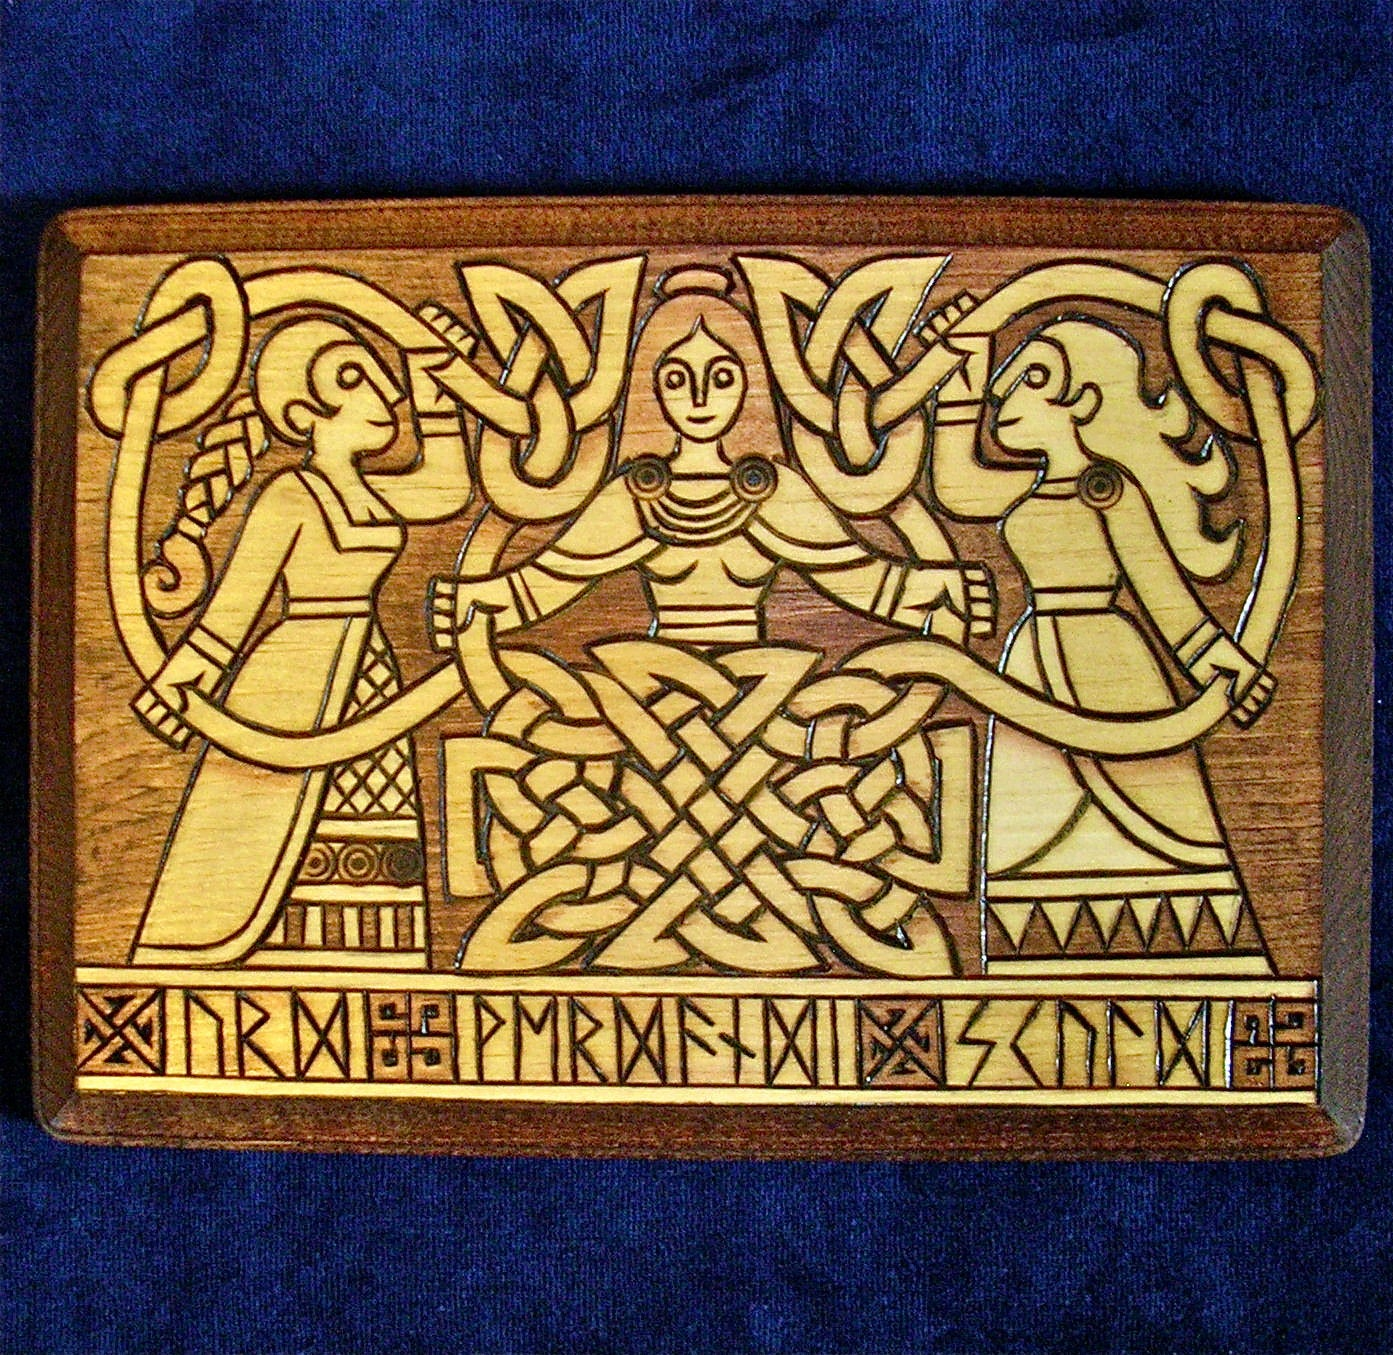
\includegraphics[trim={0 0 0 3cm},clip, width=1.5\textwidth]{figures/Others/il_fullxfull.354517109_sgyq.jpg}} % Override the page setting and occupy it all.

            % Fill the rest of the page
            \vfill  
            
        %\end{flushleft}
        \end{left}
    }  % There is an error here which complain that \begin{left} is math mode and is not closed with $$. It works fine, ignore it.
\end{center}
\cleardoublepage



%---------------------------------------------------------------------------
% Preamble
%
% This part is just for enumerating the beginning with Roman numbers. This
% includes the Preface, Acknowledgements, ...
%---------------------------------------------------------------------------
\pagenumbering{roman} 				% Begin Roman page numbering (i,ii,...)



%---------------------------------------------------------------------------
% Preface
%---------------------------------------------------------------------------
\chapter*{Preface}
    \addcontentsline{toc}{chapter}{Abstract}

        We believe that every individual, regardless of their background knowledge, should have the opportunity to engage with and appreciate the multifaceted and interdisciplinary aspects of this research. The main Ph.D. thesis document takes for granted that the readers are expert knowledge in all interdisciplinary fields which are analyzed throughout the document. This is a challenging assumption given the variety of topics discussed across the documents and the different academic backgrounds of all possible readers. 

        We understand the importance of making complex concepts accessible to a wider audience, especially to students and parents who collaborated in granting us access to their medical data. This complementary document is specifically designed to bridge the gap between advanced specialized knowledge and a more general understanding of the subject. We hope to ensure that both the general public and university individuals who haven't followed up on the topics since high school can grasp the key ideas and concepts being explored.
        
        Throughout this document, we will present key concepts behind bacteria functions with particular detail to \gls{staph}, the immune system, inflammation, vitamin D, and \gls{otc}. As well as to expand a bit more on the different mathematical backgrounds of graph theory and network analysis.

        Rafael Adolfo Nozal Cañadas

    \cleardoublepage

%---------------------------------------------------------------------------
% LIST OF ABBREVIATIONS
%
% These are displayed in alphabetical order
%---------------------------------------------------------------------------
% \chapter*{List of abbreviations}
\addcontentsline{toc}{chapter}{List of abbreviations}

\printglossary[type=\acronymtype,title=Abbreviations]

%---------------------------------------------------------------------------
% TABLE OF CONTENT
%
% This is generated automatically, you don't need to write anything
%---------------------------------------------------------------------------
\setcounter{tocdepth}{4}            % Sets the number of section levels in the table of contents to 4
\tableofcontents                    % Creates the table of contents
\cleardoublepage                    % Ends the current page


%---------------------------------------------------------------------------
% Chapters
%---------------------------------------------------------------------------
\pagestyle{fancy}               	% Fancy headings
\pagenumbering{arabic}				% Begin arabic page numbering (1,2,...)
\setlength{\parindent}{20pt}        % Sets default paragraph indentation to 20 pt 

% Introduction to networks
%*****************************************
\chapter{Social Networks}\label{ch:networks}
%*****************************************

%*****************************************
\section{Introduction}
%*****************************************

    \begin{figure}[H]
        \centering
            \includegraphics[width=0.9\linewidth]{figures/Networks/kroni2.png} 
        \caption{Königsberg according to an engraving by Joachim Bering from 1613, source \url{https://upload.wikimedia.org/wikipedia/commons/1/15/Koenigsberg\%2C\_Map\_by\_Bering\_1613.jpg}. Blue tones for the river Pregel, and orange tones for the bridges have been added for better visualization. The original names in the legend have also been added for context.}
        \label{figure:networkBridges}
    \end{figure}


A famous historical puzzle was raised by Carl Leonhard Gottlieb Ehler, the mayor of Danzig (now Gdańsk), to Leonhard Euler in 1736. The problem proposal was like this. In the city of Königsberg in Prussia (now Kaliningrad, Russia) there are seven bridges crossing the Pregel river. Starting anywhere you want in the city, how to transverse the 7 bridges crossing each bridge only once. Reaching an island or mainland bank other than via bridges, or accessing a bridge without crossing it is not permitted.

Euler was annoyed by this proposal and expressed so in a letter to the mayor: \textit{"...Thus you see, most noble Sir, how this type of solution bears little relationship to mathematics, and I do not understand why you expect a mathematician to produce it, rather than anyone else, for the solution, is based on reason alone, and its discovery does not depend on any mathematical principle.  Because of this, I do not know why even questions that bear so little relationship to mathematics are solved more quickly by mathematicians than by others."}

Even though Euler found the problem very easy, he was curious about the mathematical foundation behind it. He wrote to the Italian mathematician Giovanni Marinoni: \textit{"This question is so banal, but seemed to me worthy of attention in that geometry, nor algebra, nor even the art of counting was sufficient to solve it. In view of this, it occurred to me to wonder whether it belonged to the geometry of position which Leibniz had once so much longed for. And so, after some deliberation, I obtained a simple, yet completely established, rule with whose help one can immediately decide for all examples of this kind, with any number of bridges in any arrangement, whether such a round trip is possible, or not..."}

Nevertheless, Euler proved that the problem had no solution, and by doing so he invented a new branch of mathematics now known as graph theory. Euler realized that the details of Königsberg were irrelevant, and only the masses of land and the bridges matter. Turning a complicated structure of a city into a very simple graph. A temporal solution was found in April 1942 when two of the bridges were blown up during World War II.



%*****************************************
\section{Graph theory}
%*****************************************

\subsection{Introduction}

Graph theory is a branch of mathematics that studies the properties and applications of graphs. A graph is a mathematical structure consisting of a set of vertices (also referred to as nodes) and a set of edges of these vertices. It is a fascinating subject with numerous practical applications in several fields including physical network connections in computer science, optimizing logistics in transportation, or in our case measuring the influence of peers in social networks.

    \begin{figure}[H]
        \centering
            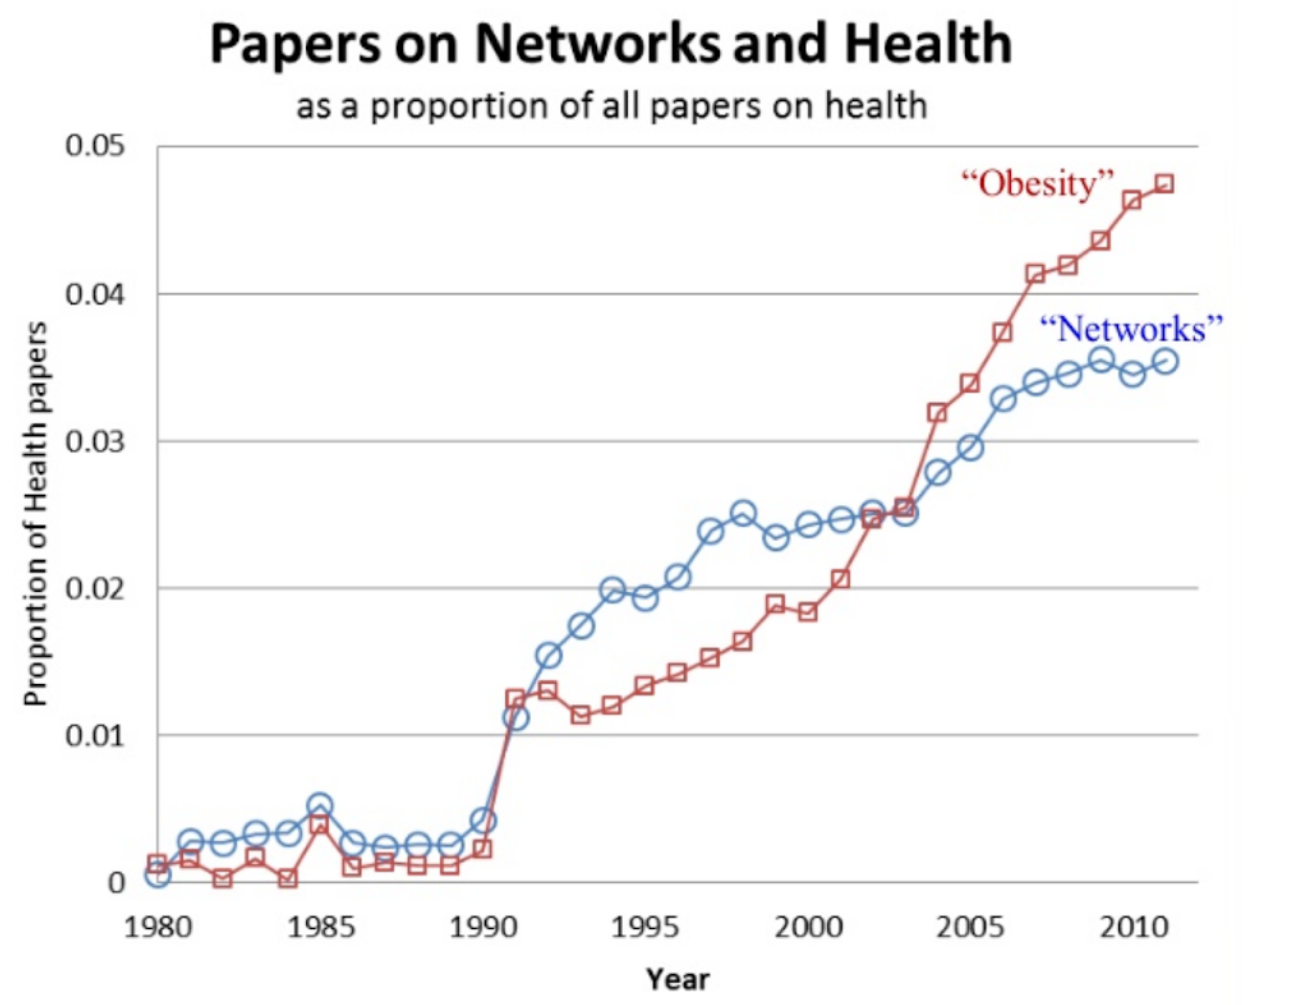
\includegraphics[width=0.7\linewidth]{figures/Networks/papersSocial.png} 
        \caption{Proportion of papers published about networks on the topic of health across the years, in comparison with the number of papers published on obesity. Reproduced from \url{https://www.sciencedirect.com/referencework/9780080970875/international-encyclopedia-of-the-social-and-behavioral-sciences}}
        \label{figure:networkNetworkRise}
    \end{figure}

Graphs provide an abstract representation of the relationships between objects, which may be used to find paths, network flow, connectivity, and more which we will discuss later on. In this context, we are going to talk about graphs and networks interchangeably. 

A graph has the following mathematical definition: \label{eq:graph}
    \begin{equation}
        G = (V,E) 
    \end{equation}
Where G is the graph, V is the set of vertices, and E is the set of edges. In figure \ref{figure:networkExampleBasic}, we define G as V = \{A, B, C, D, E, F, G, H, I, J\} and E = \{ \{A,D\}, \{B,C\}, \{C,A\}, \{C,B\}, \{D,G\}, \{E,D\}, \{F,G\}, \{F,I\}, \{G,F\}, \{H,G\}, \{J,F\} \}

\subsection{ Nodes }

A node or vertex is the fundamental element of a network. Is usually represented as a point with lines, known as edges, coming out of it, which connect it with other nodes in the network. Each node represents one elemental object in the network, which in our case is a total of 1038 students. In other contexts can be cities, computers, or any other concept.

Mathematically, we notate all nodes as V, with each individual node in a graph with lowercase variables, such as x, y, or z. The total number of nodes is notated with $|V|$. In figure \ref{figure:networkExampleBasic}, we have 10 nodes.

\subsubsection{Attributes}

Each node may have different variables, such as sex, BMI, or any other intrinsic variable proper to the object the node is representing. Each of these variables is known as the attributes of a node. Each attribute of a node is notated with subindexes, such as $x_1$, $x_2$, ... , $x_i$ , ... , $x_n$ . In figure \ref{figure:networkExampleBasic}, $A_{color} = blue$

\subsection{Edges}

An edge represents a relationship between two nodes. Our network represents a relationship of undirected friendship. The assessment of the edges is formally introduced in detail in section \cite{method:SocialNetwork}. For now, let's just comment that we have 5 types of relationships that represent the social interactions that happen between students. One is physical relationships, relationships at school, at home, at sports practice, and finally by other types of interaction. If we combine all possible edges, then we form a 6th network which we call the overall network.

Two nodes can have multiple edges with the same or different weights between them, or have none. If all edges in the graph have at least one connection to every other node, then is called a complete graph.

The mathematical definition of all edges in a graph is as follows:
    \begin{equation}
        E \subseteq  \left\{   (x,y) | (x,y) \in V^2  \land x  \neq y  \right\}
    \end{equation}
We denote the total number of edges as $|E|$. A particular edge between two nodes is simply (x,y). In figure \ref{figure:networkExampleBasic}, we have 11 edges that are directed, and in figure \ref{figure:networkExampleWeights} we have 9 edges that are undirected.

\subsubsection{Directionality}

Directionality refers to whether the edges are directed or undirected. In the case of friendship, a student may nominate others as friends while none of them nominate him back. Or they might have a strong friendship between them so everyone reciprocates everybody. Nodes can be referred to as "Ego" or "Alter". An Ego node is the node from which the relationship is emanating, and an Alter node is the node that is receiving the relationship. A phrase such as "Ego-perceived friends" means that we are focusing on a node (ego) and this node has nominated some friends.

In our network, edges are undirected, meaning that it doesn't matter which student nominates whom as a friend, in either case, there is a relationship between them.

    \begin{figure}[H]
        \centering
            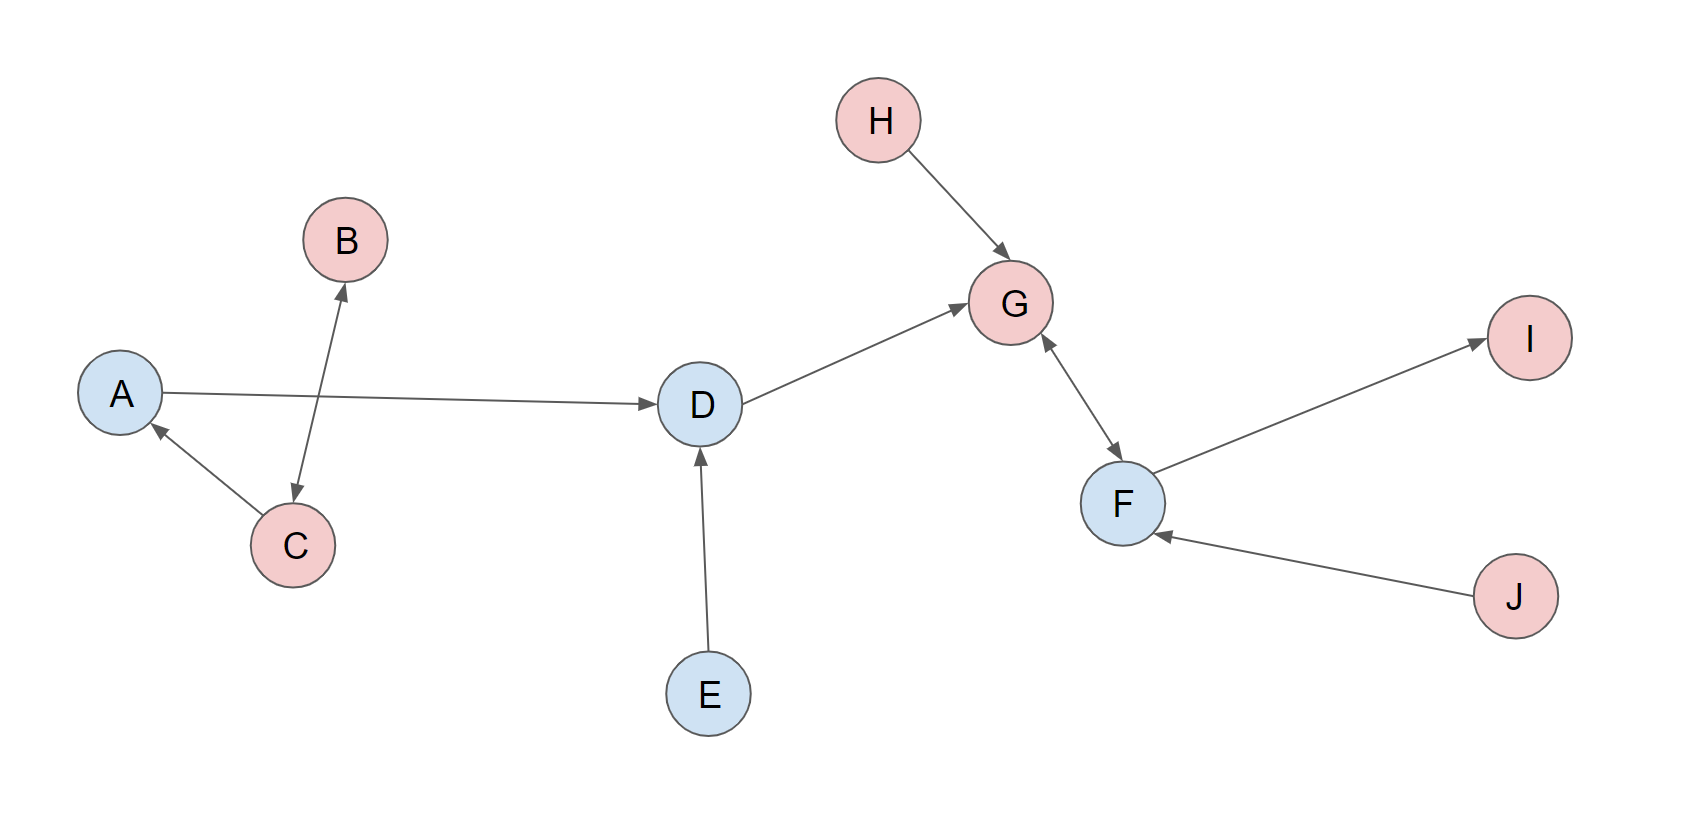
\includegraphics[width=0.7\linewidth]{figures/Networks/Concepts/directed.png} 
        \caption{An example of a network with 10 nodes labeled from A to J. Each node has a color attribute that can be either red or blue. Nodes are connected via directed relationships. Nodes B and C, and nodes G and F have a reciprocal relationship. The Laplacian representation of this matrix can be seen in table \ref{table:networkLaplacian}}
        \label{figure:networkExampleBasic}
    \end{figure}

    \begin{figure}[h!]
        \centering
            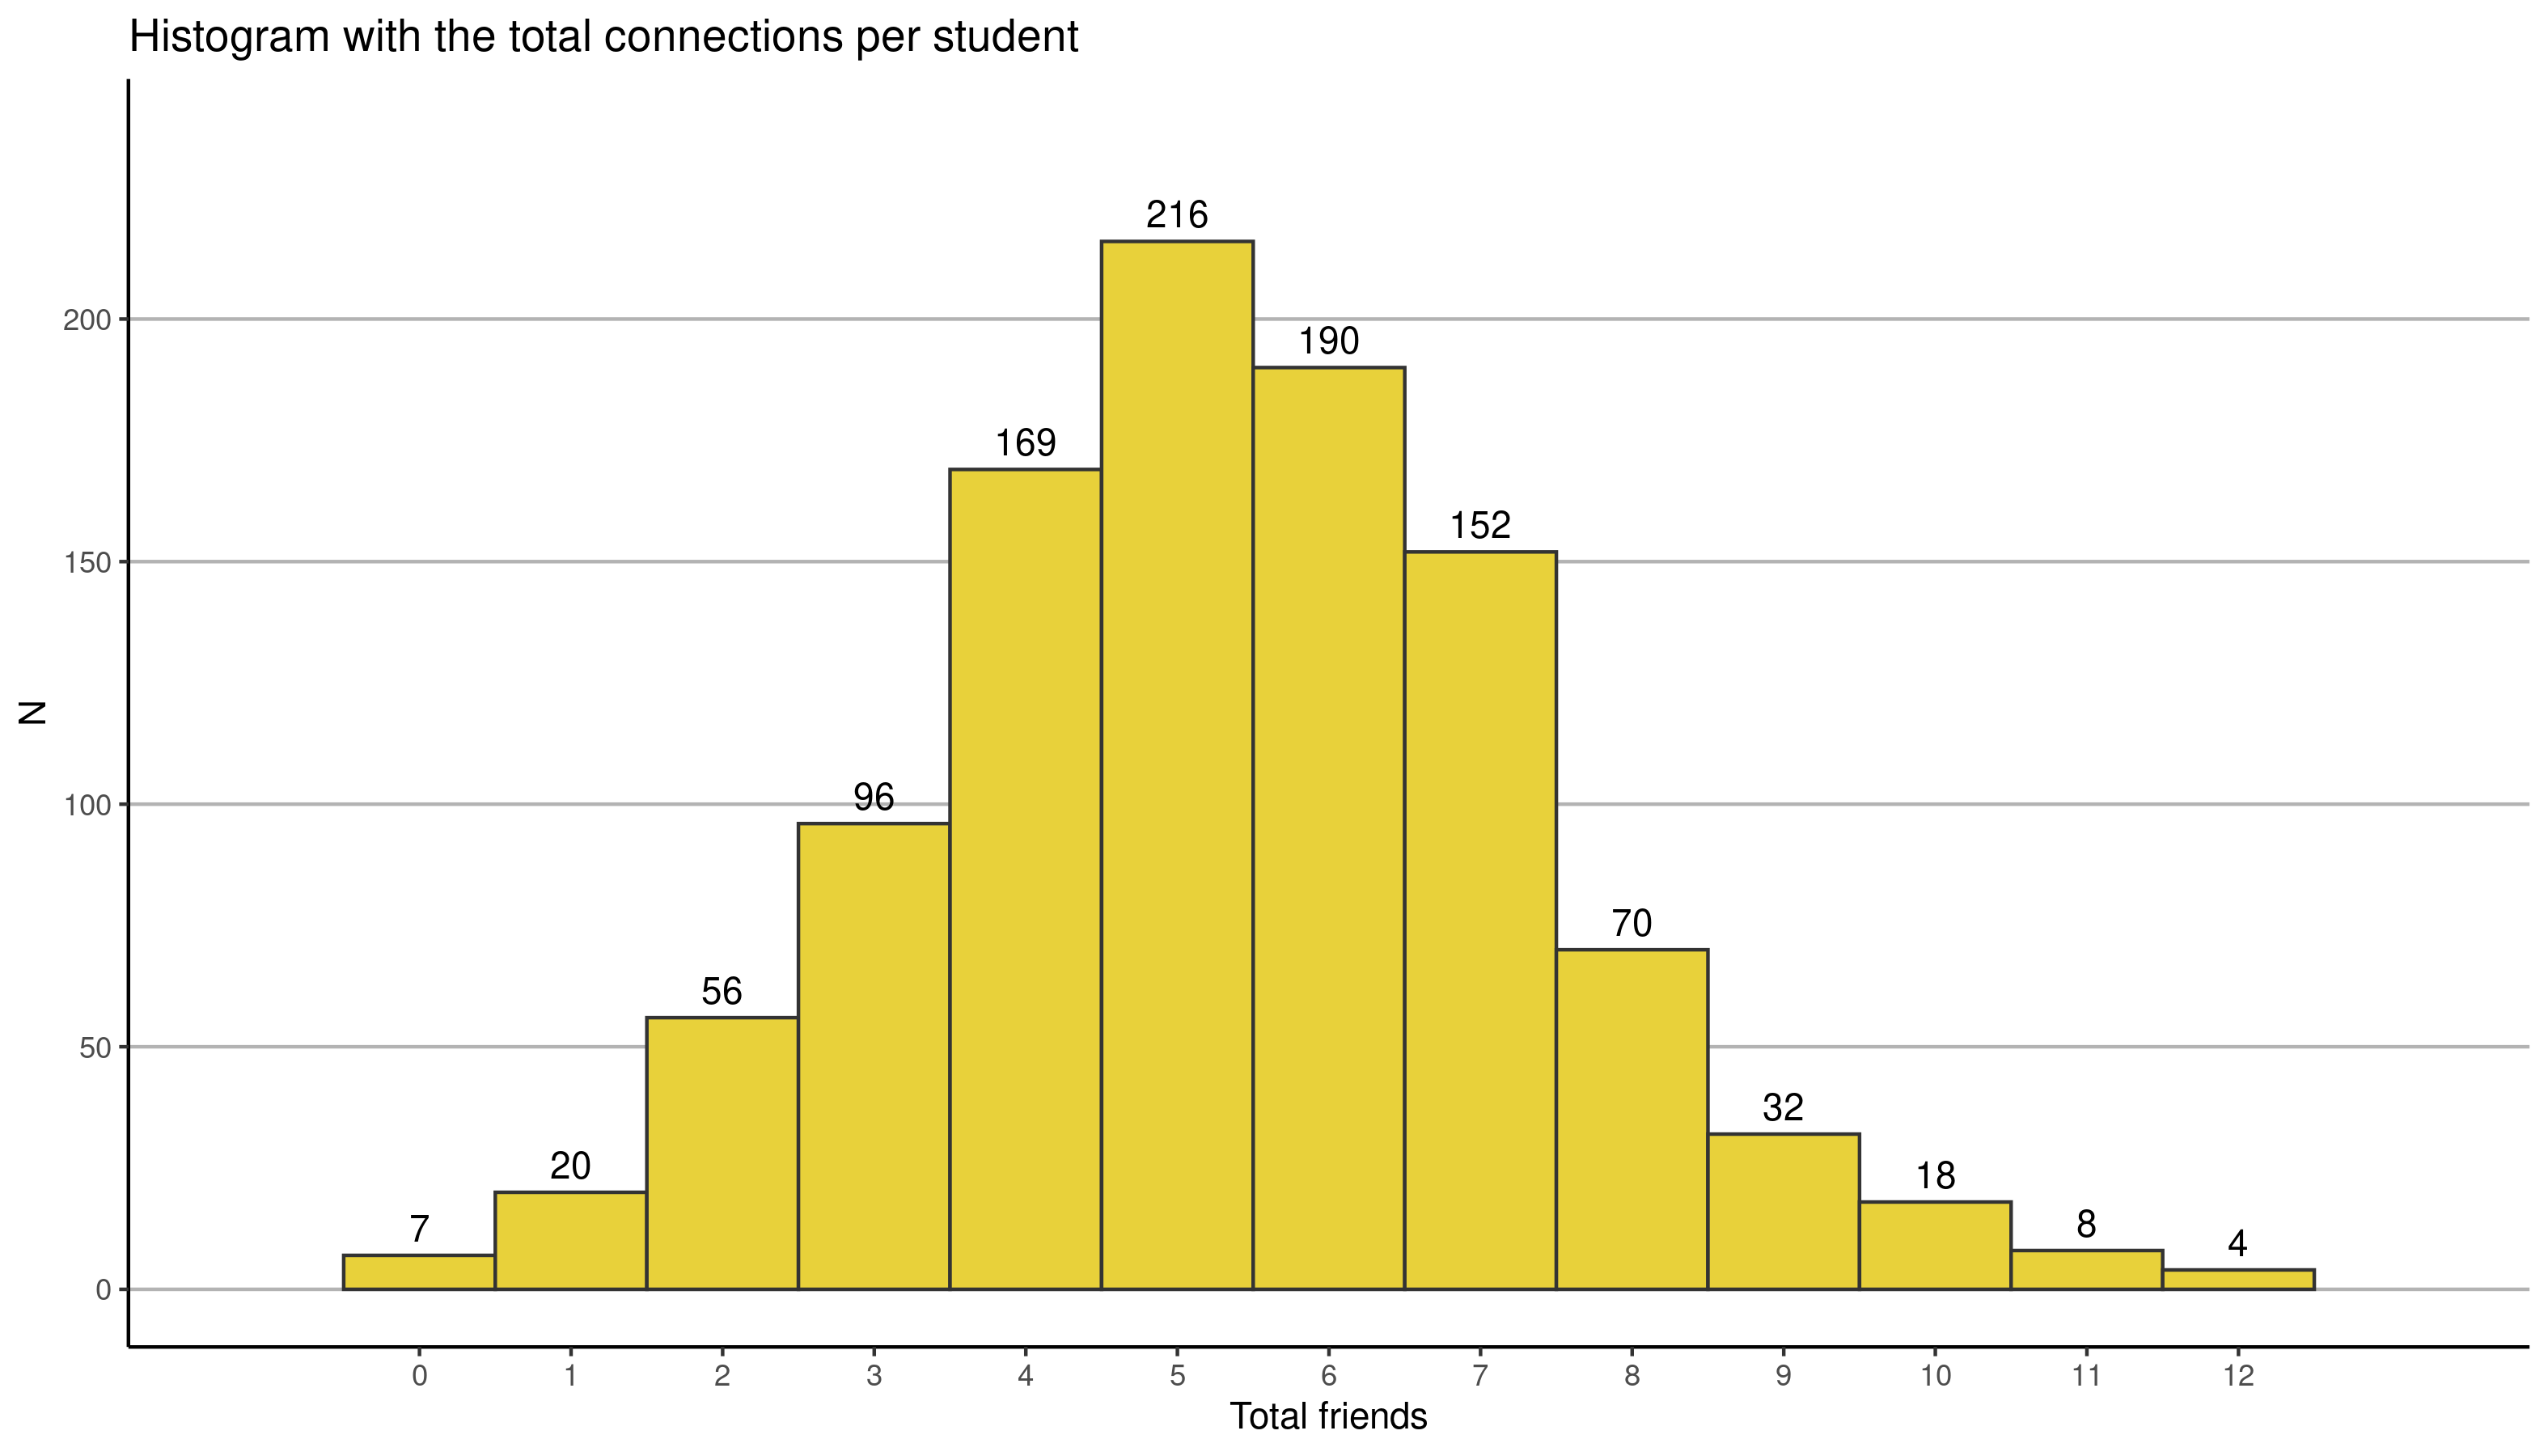
\includegraphics[width=0.7\linewidth]{figures/Networks/Histograms/Histogram_completeTable_OverallConnections.png} 
        \caption{A histogram with the total of undirected friends per student in the overall network. Some students are popular with up to 12 connections, while others are isolated with 0 connections.}
        \label{figure:networksHistogramFriendship}
    \end{figure}  

\subsubsection{Reciprocity ratio}

The reciprocity ratio is the number of edges that has a reciprocal relationship. This can only be measured in networks that are directed.

\subsubsection{Weight}

All edges have an additional property called weight. This is a variable, typically a real number, that indicates some quantifying property of the relationship. For example the distance between two cities, or how many hours per day you spend in the company of a person. By default, all edges have a weight of 1, meaning all relationships have the same importance; this is our case study.

    \begin{figure}[h!]
        \centering
            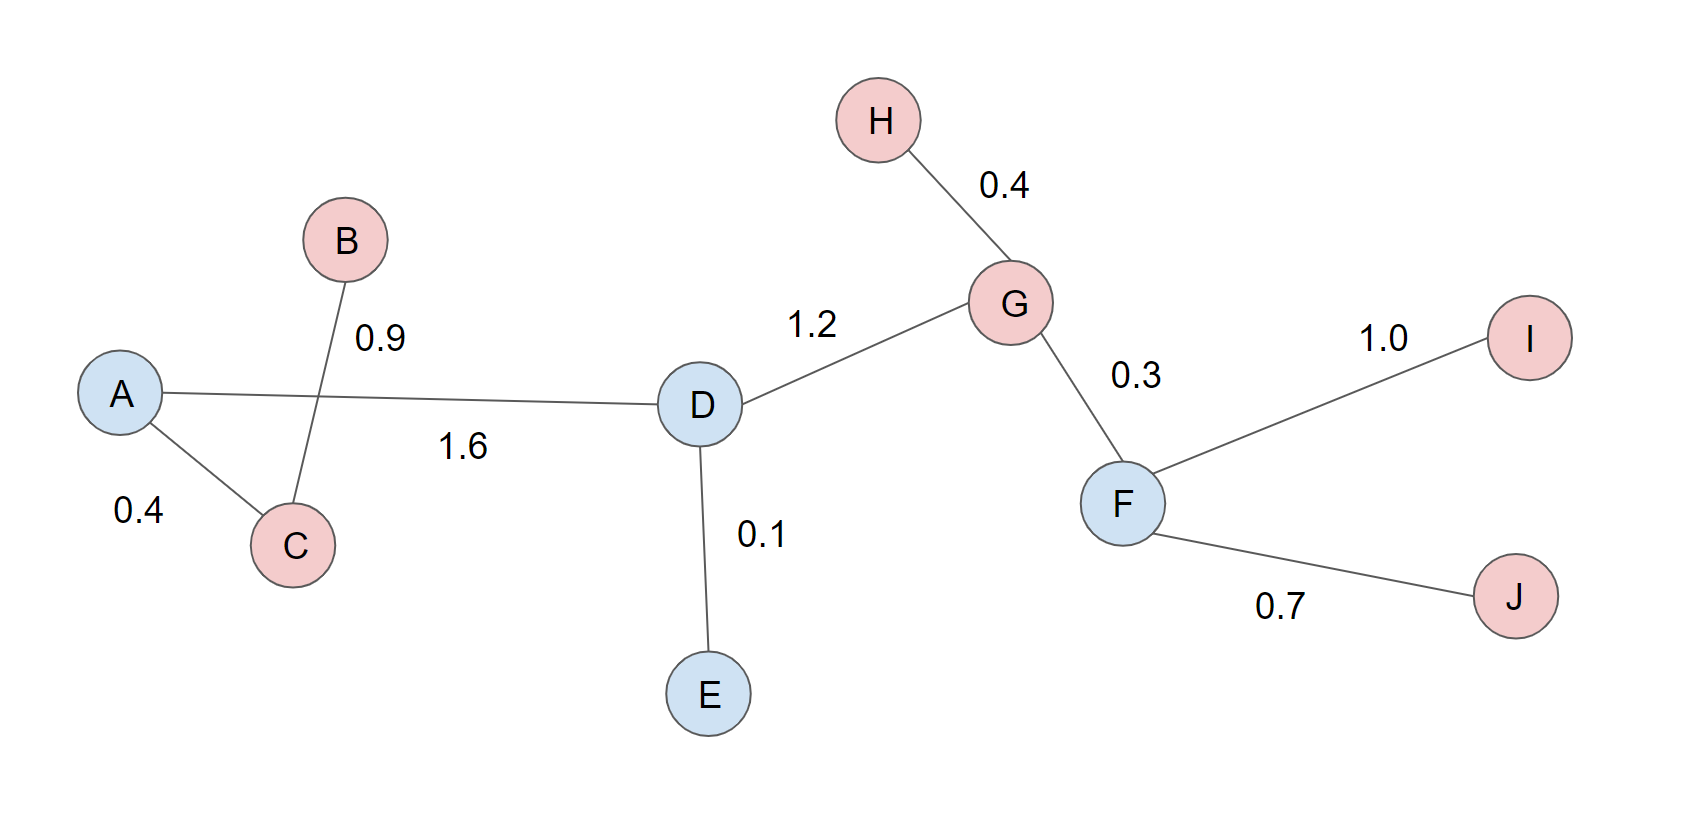
\includegraphics[width=0.7\linewidth]{figures/Networks/Concepts/edgesValues.png} 
        \caption{An example of a network with 10 nodes and weighted undirected relationships. A spring layout of this network can be seen in figure \ref{figure:networkExampleSpring}}
        \label{figure:networkExampleWeights}
    \end{figure}

Nodes that are not connected can be defined to either have a weight of zero or a weight of infinity, depending on the wording of your definition.

\subsubsection{Loop}

A relationship of a node with itself is allowed in graph theory and is called a loop. Be aware that this may not make sense in a context such as ours. Philosophically a person might be friends with himself if we define it as being happy with his life, but mathematically we don't have any use for such a definition. But it can make sense if we talk about a network of collaborations and we define a loop as authors' self-promotion. In a transportation network, a loop can represent a roundabout where a vehicle can circle around the same point.

\subsubsection{Connectivity}
\label{network:Connectivity}

Is the summation of all edges' weight. When all the nodes in the network have at least 1 connectivity is it said that the network is fully connected. There are four main methods of measuring connectivity:

\begin{itemize}
    \item \textbf{In-degree:} Summation of all the weights coming into the node.
    \item \textbf{Out-degree:} Summation of all the weights going outside the node.
    \item \textbf{Reciprocity:} Summation of weights in reciprocal edges.
    \item \textbf{Undirected:} Summation of in and out connections.
\end{itemize}

    \label{table:networkGeneralStats}
    \begin{table}[h!]    
        \centering
        \caption{Overview of all basic statistics of the six networks. From left to right, the name of the network, the total number of edges in the network, average out-degree, average in-degree, average reciprocity, the average number of connections per node, and the average distance between non-isolated nodes. Notice that average out-degree and average in-degree must have the same value, but the standard deviation varies. Reciprocity in "Overall" is increased because nodes can nominate in one network but receive the nomination from the same friend from another network.}
        \footnotesize
        \renewcommand{\arraystretch}{1.7}
            \begin{tabular}{r|rrrrrr} 
            \hline
            
            \rowcolor[rgb]{1,1,0.78} \multicolumn{1}{c}{Name} & \multicolumn{1}{c}{Edges} & \multicolumn{1}{c}{$\overline{Out}$} & \multicolumn{1}{c}{$\overline{In}$} & \multicolumn{1}{c}{$\overline{Reciprocity}$} & \multicolumn{1}{c}{$\overline{Connections}$} & \multicolumn{1}{c}{$\overline{Distance}$}  \\ 
            \hline
            
            {\cellcolor[rgb]{1,0.808,0.576}}Overall           & 3767              & 3.63 ± 1.32 & 3.63 ± 2.11 & 1.92 ± 1.27 & 5.34 ± 2.04 & 8.00                                        \\
            {\cellcolor[rgb]{1,0.808,0.576}}Physical          & 2823              & 2.72 ± 1.71 & 2.72 ± 1.96 & 1.25 ± 1.20 & 4.18 ± 2.19 & 9.91                                     \\
            {\cellcolor[rgb]{1,0.808,0.576}}School            & 2979              & 1.20 ± 1.35 & 1.20 ± 1.25 & 0.49 ± 0.75 & 1.92 ± 1.66 & 6.90                                      \\
            {\cellcolor[rgb]{1,0.808,0.576}}Sport             & 598               & 2.87 ± 1.59 & 2.87 ± 1.85 & 1.42 ± 1.20 & 4.32 ± 1.92 & 13.73                                    \\
            {\cellcolor[rgb]{1,0.808,0.576}}Home              & 1247              & 0.58 ± 1.11 & 0.58 ± 1.04 & 0.18 ± 0.56 & 0.97 ± 1.48 & 3.58                                     \\
            {\cellcolor[rgb]{1,0.808,0.576}}Other             & 1095              & 1.05 ± 1.47 & 1.05 ± 1.11 & 0.26 ± 0.58 & 1.85 ± 1.68 & 7.08                                    
            \end{tabular}
    \end{table}

\subsubsection{Laplacian matrix}

A graph can be represented as a matrix, in which each cell combination of row and column represents an edge between two nodes. This is known as the Laplacian matrix of a graph, or simply the matrix.

\label{table:networkLaplacian}
\begin{table}[h!]

    \centering

    \caption{Example of a Laplacian matrix corresponding to figure \ref{figure:networkExampleBasic}. Summation by row represents the out-degree. Summation by columns represents the in-degree. Cells that are symmetrical from the main diagonal, represent reciprocal relationships.}
    
    \begin{tabular}{|c|cccccccccc|} 
    \hhline{~----------|}
    \multicolumn{1}{c|}{}           & \multicolumn{10}{c|}{{\cellcolor[rgb]{1,0.988,0.62}}Node receiving the edge}                                                                                                                                                                                                                                         \\ 
    \hhline{~----------|}
    \multicolumn{1}{c|}{}           & {\cellcolor[rgb]{1,1,0.78}}A & {\cellcolor[rgb]{1,1,0.78}}B & {\cellcolor[rgb]{1,1,0.78}}C & {\cellcolor[rgb]{1,1,0.78}}D & {\cellcolor[rgb]{1,1,0.78}}E & {\cellcolor[rgb]{1,1,0.78}}F & {\cellcolor[rgb]{1,1,0.78}}G & {\cellcolor[rgb]{1,1,0.78}}H & {\cellcolor[rgb]{1,1,0.78}}I & {\cellcolor[rgb]{1,1,0.78}}J  \\ 
    \hline
    {\cellcolor[rgb]{0.604,1,0.6}}A & 0                            & 0                            & 0                            & 1                            & 0                            & 0                            & 0                            & 0                            & 0                            & 0                             \\
    {\cellcolor[rgb]{0.604,1,0.6}}B & 0                            & 0                            & 1                            & 0                            & 0                            & 0                            & 0                            & 0                            & 0                            & 0                             \\
    {\cellcolor[rgb]{0.604,1,0.6}}C & 1                            & 1                            & 0                            & 0                            & 0                            & 0                            & 0                            & 0                            & 0                            & 0                             \\
    {\cellcolor[rgb]{0.604,1,0.6}}D & 0                            & 0                            & 0                            & 0                            & 0                            & 0                            & 1                            & 0                            & 0                            & 0                             \\
    {\cellcolor[rgb]{0.604,1,0.6}}E & 0                            & 0                            & 0                            & 1                            & 0                            & 0                            & 0                            & 0                            & 0                            & 0                             \\
    {\cellcolor[rgb]{0.604,1,0.6}}F & 0                            & 0                            & 0                            & 0                            & 0                            & 0                            & 1                            & 0                            & 1                            & 0                             \\
    {\cellcolor[rgb]{0.604,1,0.6}}G & 0                            & 0                            & 0                            & 0                            & 0                            & 1                            & 0                            & 0                            & 0                            & 0                             \\
    {\cellcolor[rgb]{0.604,1,0.6}}H & 0                            & 0                            & 0                            & 0                            & 0                            & 0                            & 1                            & 0                            & 0                            & 0                             \\
    {\cellcolor[rgb]{0.604,1,0.6}}I & 0                            & 0                            & 0                            & 0                            & 0                            & 0                            & 0                            & 0                            & 0                            & 0                             \\
    {\cellcolor[rgb]{0.604,1,0.6}}J & 0                            & 0                            & 0                            & 0                            & 0                            & 1                            & 0                            & 0                            & 0                            & 0                             \\
    \hline
    \end{tabular}
\end{table}

%https://en.wikipedia.org/wiki/Laplacian_matrix

\subsubsection{Distance}

A distance is the summation of the edge's weights between two nodes, whether they are directly connected or have some intermediary nodes between them. Distance is not necessarily unique, a couple of nodes can have several different distances between them. If two nodes have no connection, the distance is equal to infinity. If your network allows for edges forming loops then you will also have an infinite combination of nodes and thus infinite possible distances.

\subsubsection{Path}

A path is the minimum weighted distance between two nodes. The path to the same node can be 0, or another value specified in a loop. A path can be negative if the graph is allowed to have negative distances. A path can be infinite if, for example, two nodes are unreachable from one to another. A directed graph can have different path lengths from any given pair of two nodes.

    \begin{figure}[h]
        \centering
            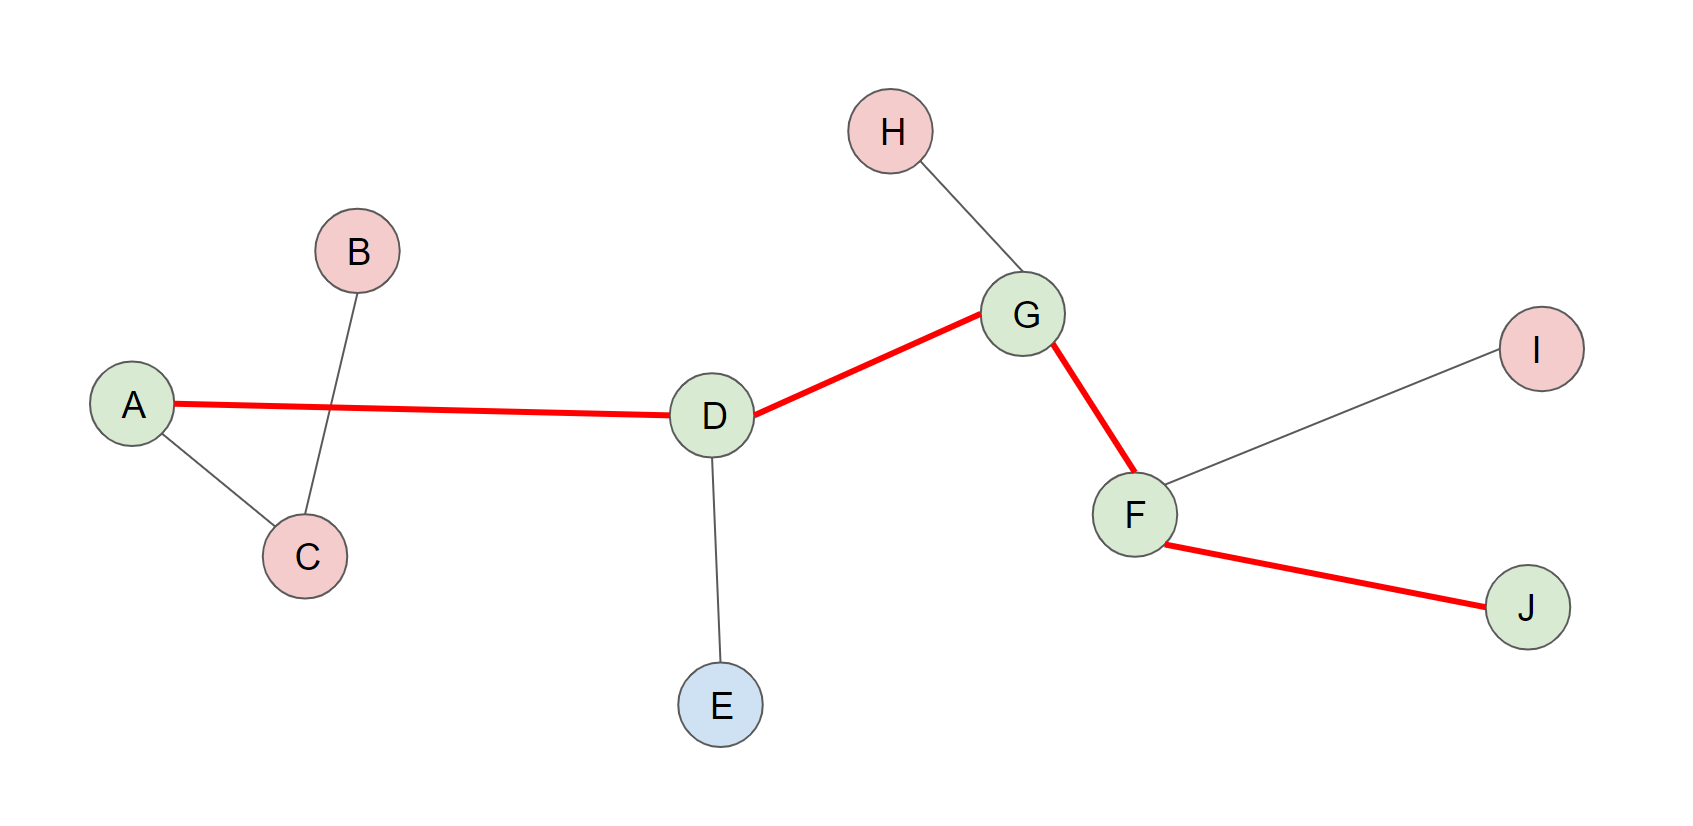
\includegraphics[width=0.7\linewidth]{figures/Networks/Concepts/path.png} 
        \caption{An example of a path. Node A can reach node J following the red highlighted edges and passing through the green highlighted nodes. All the edges weigh the same value (1), so the path is equal to 4.}
        \label{figure:networkPath}
    \end{figure}

\subsection{Network}

%https://eehh-stanford.github.io/SNA-workshop/graphs.html#dyads-triads-and-other-local-structures

% https://www.cambridge.org/core/books/abs/social-network-analysis/dyads/52A3652CD28CA469BA95572A1B714EC3 Book about social network for references.

% ERGM models, there is nothing done with this https://appliednetsci.springeropen.com/articles/10.1007/s41109-021-00403-5

\subsubsection{Isomorphic}
\label{network:isomorphic}

Two graphs are said to be isomorphic if they have the same edges and nodes if we remove the attributes of all nodes in both graphs. This is also known as network topology.

\subsubsection{Network motifs}

A set of two nodes is called a diad. A set of three nodes is called a triad. A set of four nodes is called a tetrad. An undirected diad can have only two states, either the two nodes share an edge, or they don't. A directed diad can have 4 states: no common edge, the edge from A to B, the edge from B to A, reciprocal edges from A to B, and B to A. Similarly, triads and tetrads have a limited amount of combinations of edges and no edges between their nodes. All of these examples are called network motifs.

Networks that have the same context, for example, how animals share spaces in the wilderness, and how followers are distributed in internet social networks, tend to have the same distribution of motifs. Sometimes is useful to compare the motif count with other network motif counts to check if their structure is similar. Other time is interesting to simulate a network by giving a set of probabilities for each network motif to force a specific structure.

Network motifs are an important concept in social science studies to describe the structure of the network \cite{Faust2010}, but there are better metrics on how to describe a network \cite{Faust2007}.

\subsubsection{Components}

 If no path exists that connects all nodes with all other nodes in the network it means that you have a network divided into components. A network can have isolated nodes, isolated diads, triads, or be divided into several sub-networks. Each of these cases is known as a component of a network. In figure \ref{figure:networksConnectivity} we have one network with two components. 

\subsubsection{Clusters and Communities}

Community detection is the process of discovering groups or clusters of nodes in a social network that have a high degree of connectivity within themselves, or low with other groups. There is no best algorithm and the use of each depends on the needs of the researcher:

\begin{itemize}

    \item \textbf{Modularity:} This method compares the density of different groups and is useful to compare hierarchical and overlapping communities.
    
    \item \textbf{Clustering:} This is a family of algorithms that consists of dividing groups with similar attributes. Different approaches are k-means, hierarchical clustering, or spectral clustering
    
    \item \textbf{Link-based:} This method uses the edges in the graph and measures how far you can walk from one node to another one. Communities tend to have shorter walking distances between them.

    \item \textbf{Latent variable:} These methods are somewhat similar to PCA analysis, in which we decided a number of hidden latent variables, and the algorithm groups automatically nodes based on those latent variables.

\end{itemize}

In our case, we already have the data divided in communities by high schools, down to the same class levels. And we have several attributes in each node to compare different values. As we have not done any study regarding the intricacies of each high school individually, no clustering has been applied so far other than calculating homophilies (section \ref{network:homophily}).

% https://towardsdatascience.com/an-introduction-to-graph-partitioning-algorithms-and-community-detection-29e7c962d10e?gi=ab4d5c83b911

%https://towardsdatascience.com/an-introduction-to-graph-neural-network-gnn-for-analysing-structured-data-afce79f4cfdc

% https://appliednetsci.springeropen.com/articles/10.1007/s41109-019-0248-7

% Prostitutes in China Moody, James, Jimi Adams, and Martina Morris. “Epidemic potential by sexual activity distributions.” Network Science (Cambridge University Press) 5, no. 4 (December 2017): 461–75.

% https://stackoverflow.com/questions/9471906/what-are-the-differences-between-community-detection-algorithms-in-igraph/

% https://www.r-bloggers.com/2012/06/summary-of-community-detection-algorithms-in-igraph-0-6/

% https://people.duke.edu/~jmoody77/snh/2021/CommunitiesSNH2021.nb.html

\subsubsection{Multimodal networks}

The network can be multimodal. This means that a node can connect to other nodes that are not of the same class. For example, a researcher can collaborate with other researchers, which are nodes of the same class. They publish a paper together which is another class of nodes that nevertheless connect to researchers. The paper is published in a journal which is another class. Multimodal networks are characterized as being hard to analyze due to the different meanings of the different relationships.

\section{Layout}

So far we can define a network as a table of nodes with attributes, and another table of edges and weights. Mathematically this is all we need. But for visualization purposes, there are several possibilities as to how we can spread the nodes in a typically 2D or 3D image. Proper node placement can help in creating a clear and intuitive picture making it easier to understand the relationships between the nodes. On the other hand, the emerging pattern in the network can be hidden if a poor option is chosen. This is called network layout. There are several algorithms for vertex placement. The basic categories are:

    \begin{figure}[H]
        \centering
            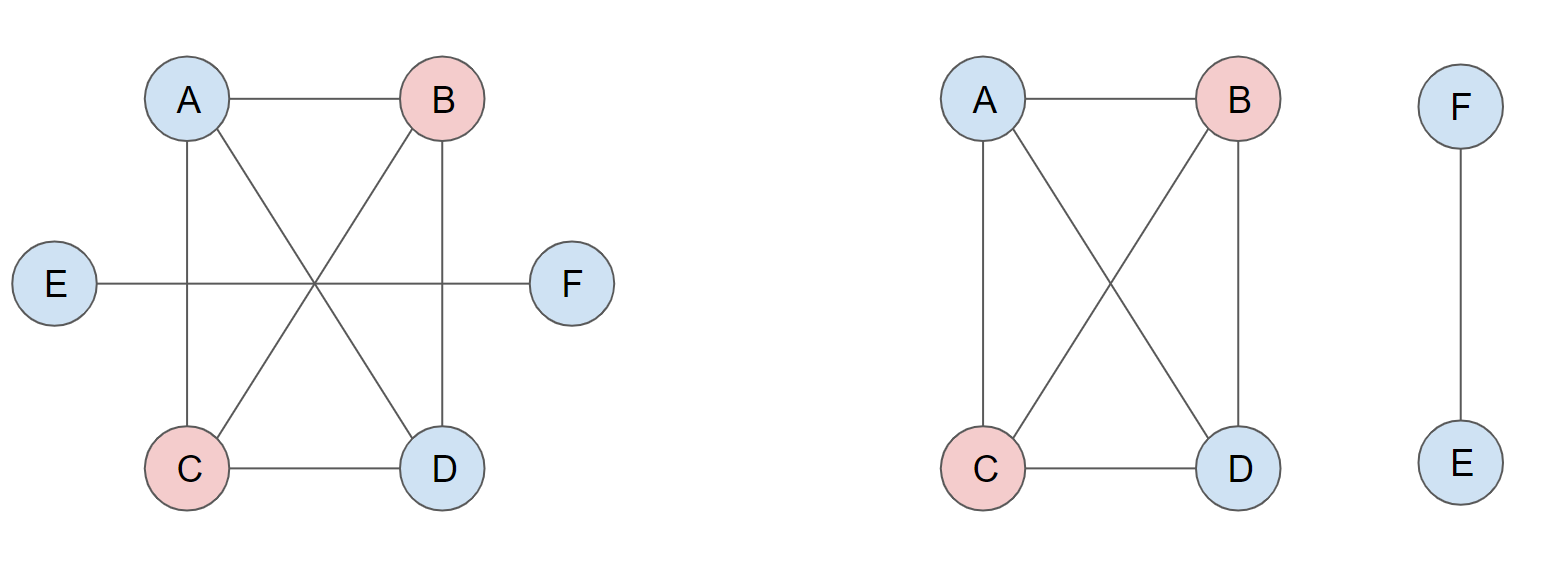
\includegraphics[width=0.7\linewidth]{figures/Networks/Layouts/isomorp.png} 
        \caption{An example of two layouts. On the left, the relationship between E and F is not clear. On the right, is obvious that E and F are disconnected from all other nodes}
        \label{figure:networkExampleLayout}
    \end{figure}

\subsection{Random}

Random placement of the nodes. Just spread the nodes around in no particular order and hope for the best.

    \begin{figure}[H]
        \centering
            \includegraphics[width=0.7\linewidth]{figures/Networks/Layouts/Graph_OverallNetwork_with_no_highlight_grid_HighSchool___grid.png} 
        \caption{Overall network placing the nodes randomly in a 2D grid. This is useful when the amount of connections is very low, but otherwise useless for visualizing patterns in this network.}
        \label{figure:networksLayoutsGRID}
    \end{figure}

\newpage

\subsection{Force directed}

This uses physics-based simulations to determine the position of nodes based on the attractive and repulsive forces between them. For example, we can imagine the nodes as electrical charges based on node properties, or the edges as springs with an elastic force proportional to the edge value.

    \begin{figure}[h!]
        \centering
            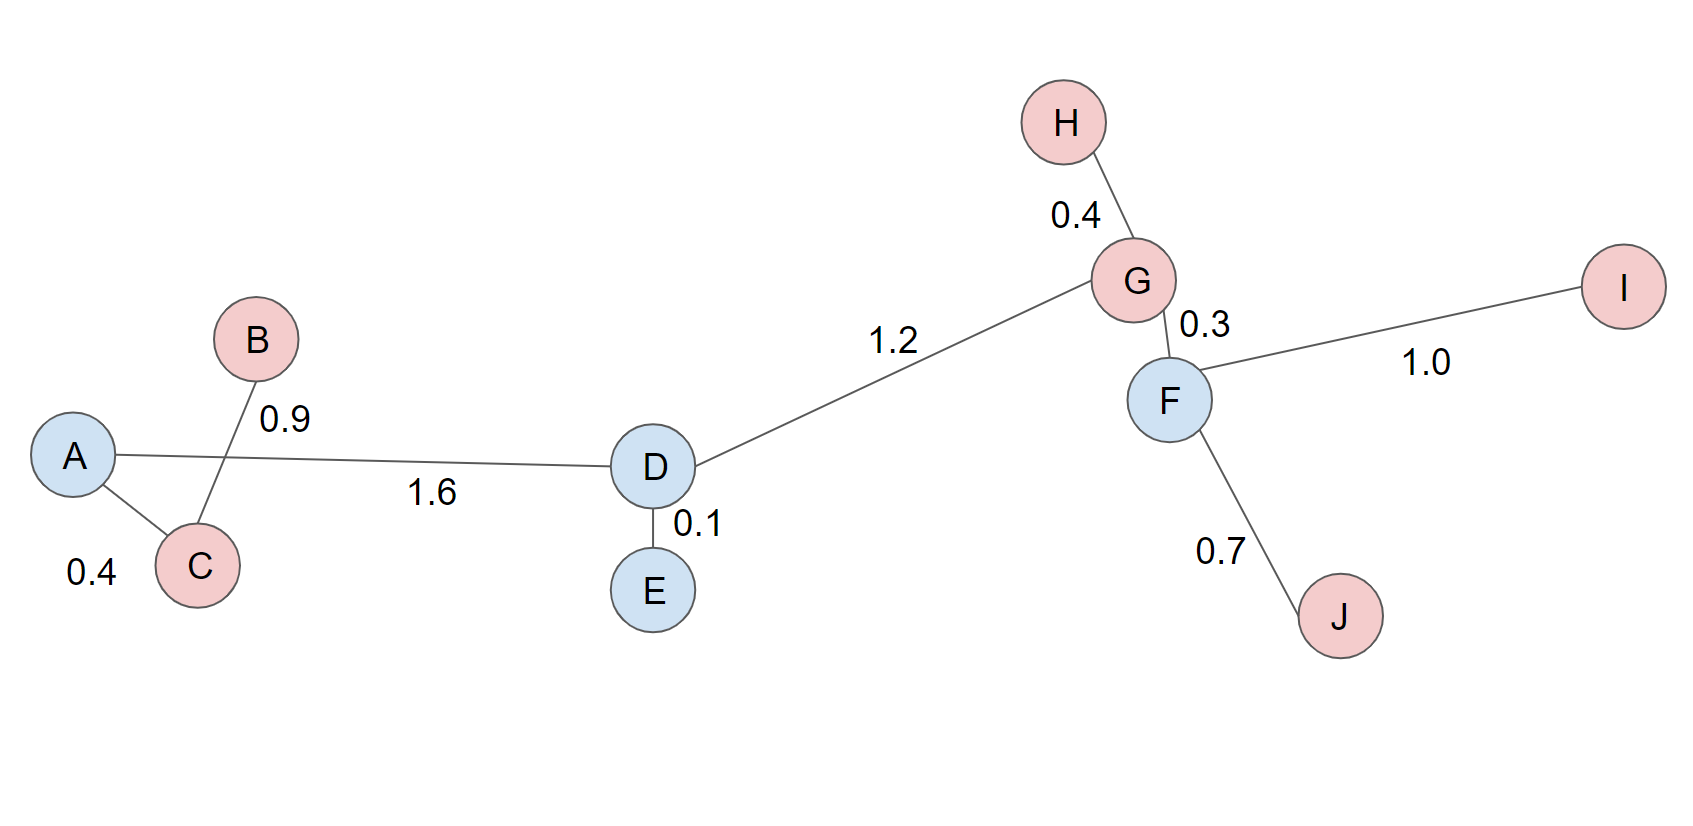
\includegraphics[width=0.7\linewidth]{figures/Networks/Concepts/edgesSpring.png} 
        \caption{An example of a network with 10 nodes and weighted undirected relationships with a spring layout. Nodes with smaller weights are brought closer together in the 2D space as if the edges were acting as springs with greater or lower spring force equilibrium alike to Hooke’s law.}
        \label{figure:networkExampleSpring}
    \end{figure}

\subsection{Hierarchical}

Hierarchical layouts tend to put important nodes on top, and less important nodes on the bottom. This type of layout only makes sense when you actually have a hierarchical relationship. Common in multi-modal networks, or where there are many triads with only two nodes connecting. Hierarchy would also mean that nodes' placement in the y-axis has some meaning of importance.

    \begin{figure}[h!]
        \centering
            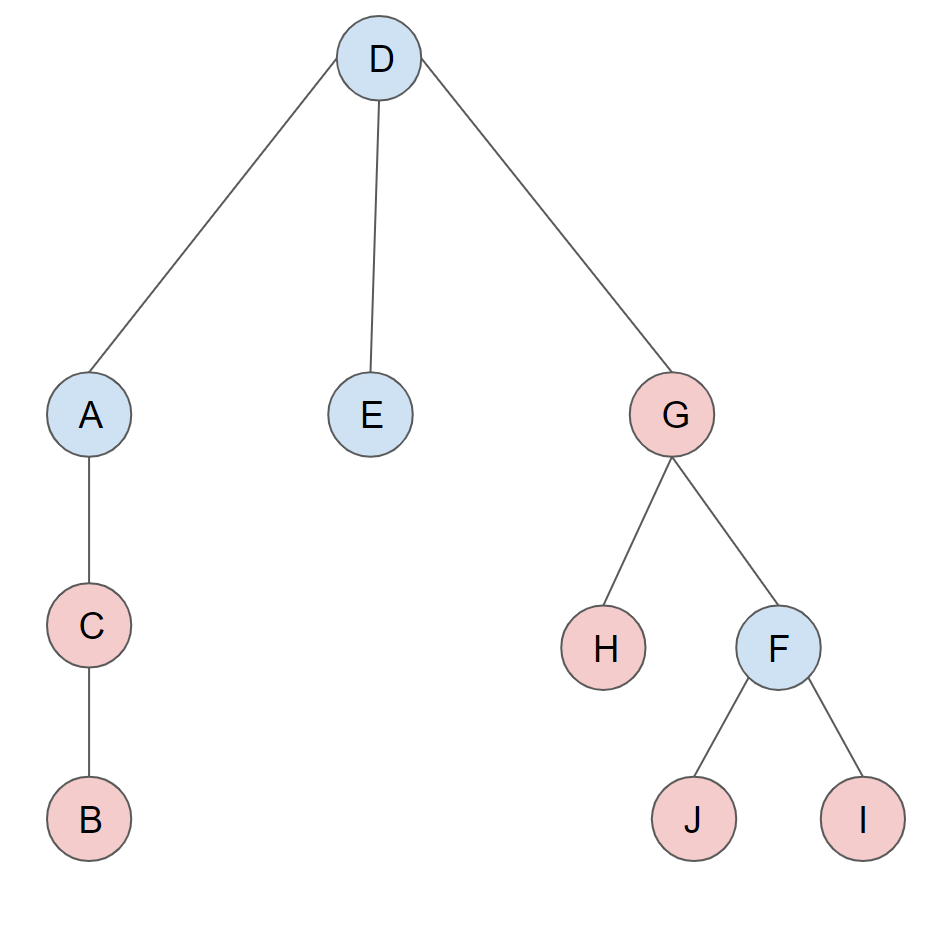
\includegraphics[width=0.5\linewidth]{figures/Networks/Layouts/hirearchy.png} 
        \caption{Our recurrent example of a network layout in a hierarchical pattern. In this example is highlighted that D is a very important node in the network, and is placed on top.}
        \label{figure:networkExampleHierarchy}
    \end{figure}

\newpage

\subsection{Spectral}

A way that minimizes a particular energy function derived from the graph's Laplacian matrix. The spectral placement technique is designed to produce graph layouts that not only look aesthetically pleasing but also provide some semantic information about the underlying network

\subsubsection{DRL}

    \begin{figure}[h!]
        \centering
            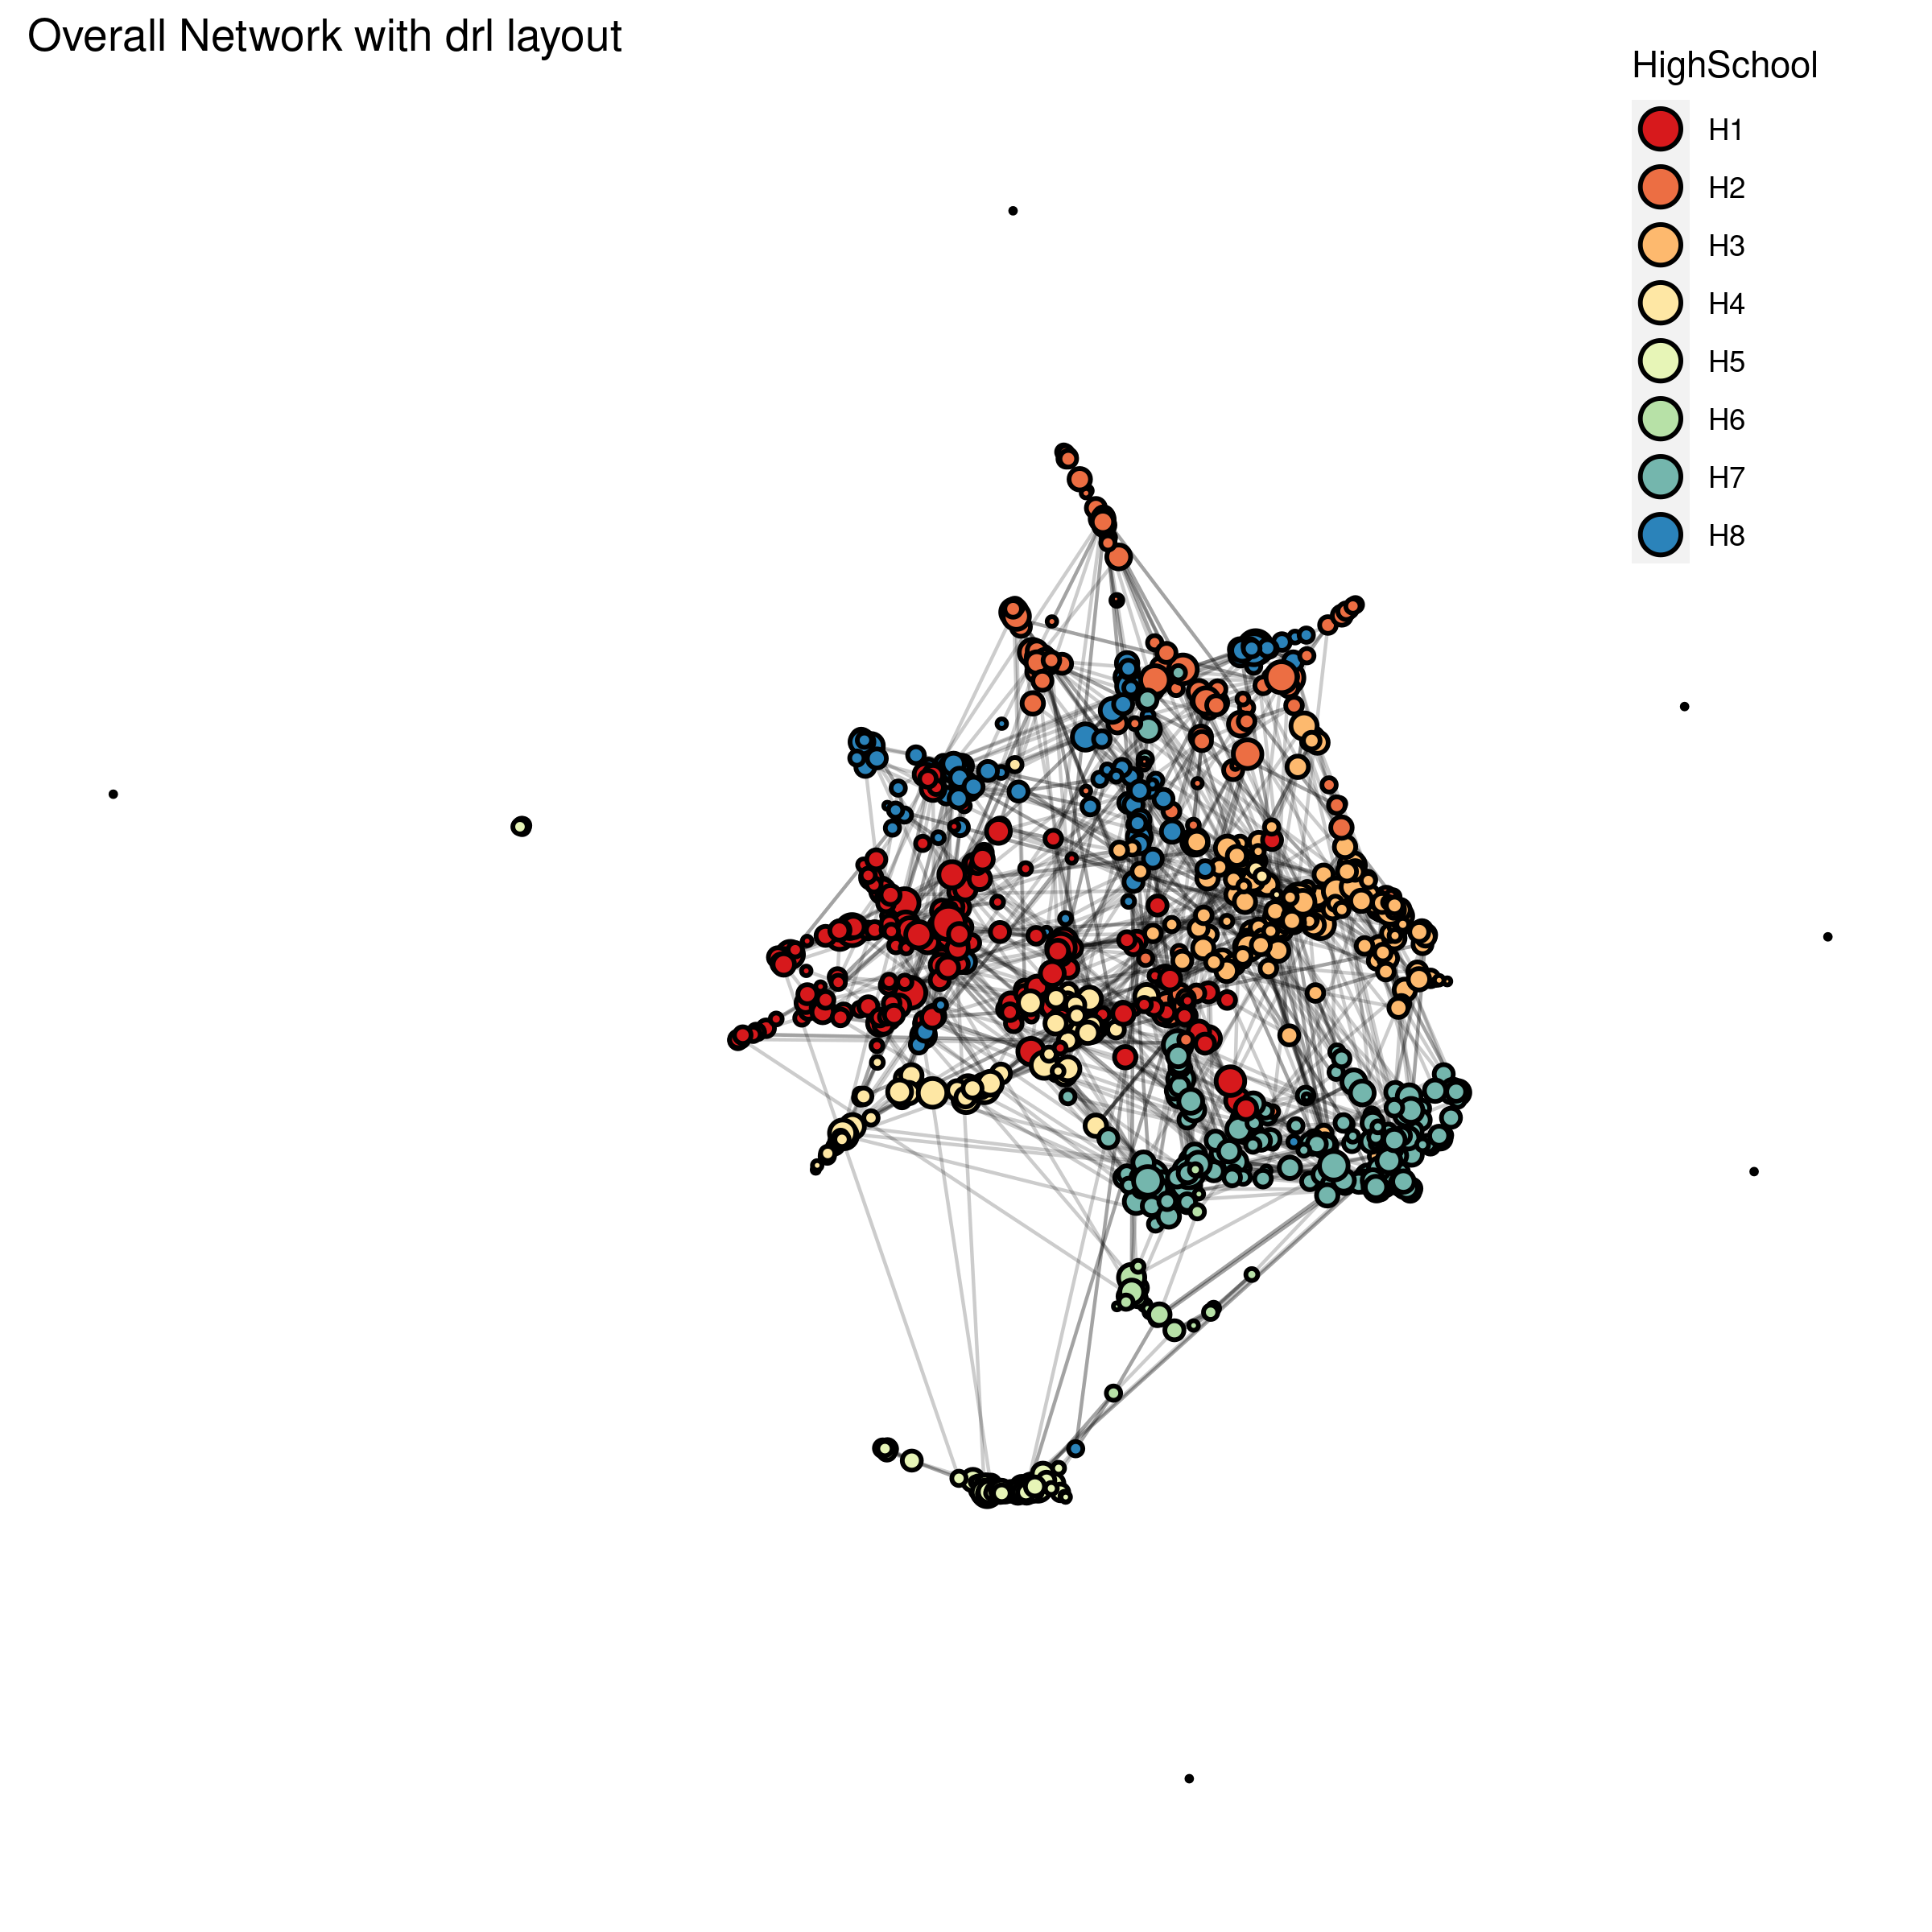
\includegraphics[width=0.7\linewidth]{figures/Networks/Layouts/Graph_OverallNetwork_with_no_highlight_drl_HighSchool___drl.png} 
        \caption{Overall network with a \gls{drl} algorithm  \cite{osti_1145621} . The layout produced by a DRL is hierarchical in nature and is well-suited for presenting large-scale graphs with a clear structure. In our case, it clusters high schools somewhat together but is not the best choice for our network.}
        \label{figure:networksLayoutsDRL}
    \end{figure}

    \newpage

\subsubsection{Fruchterman - Reingold}

    \begin{figure}[h!]
        \centering
            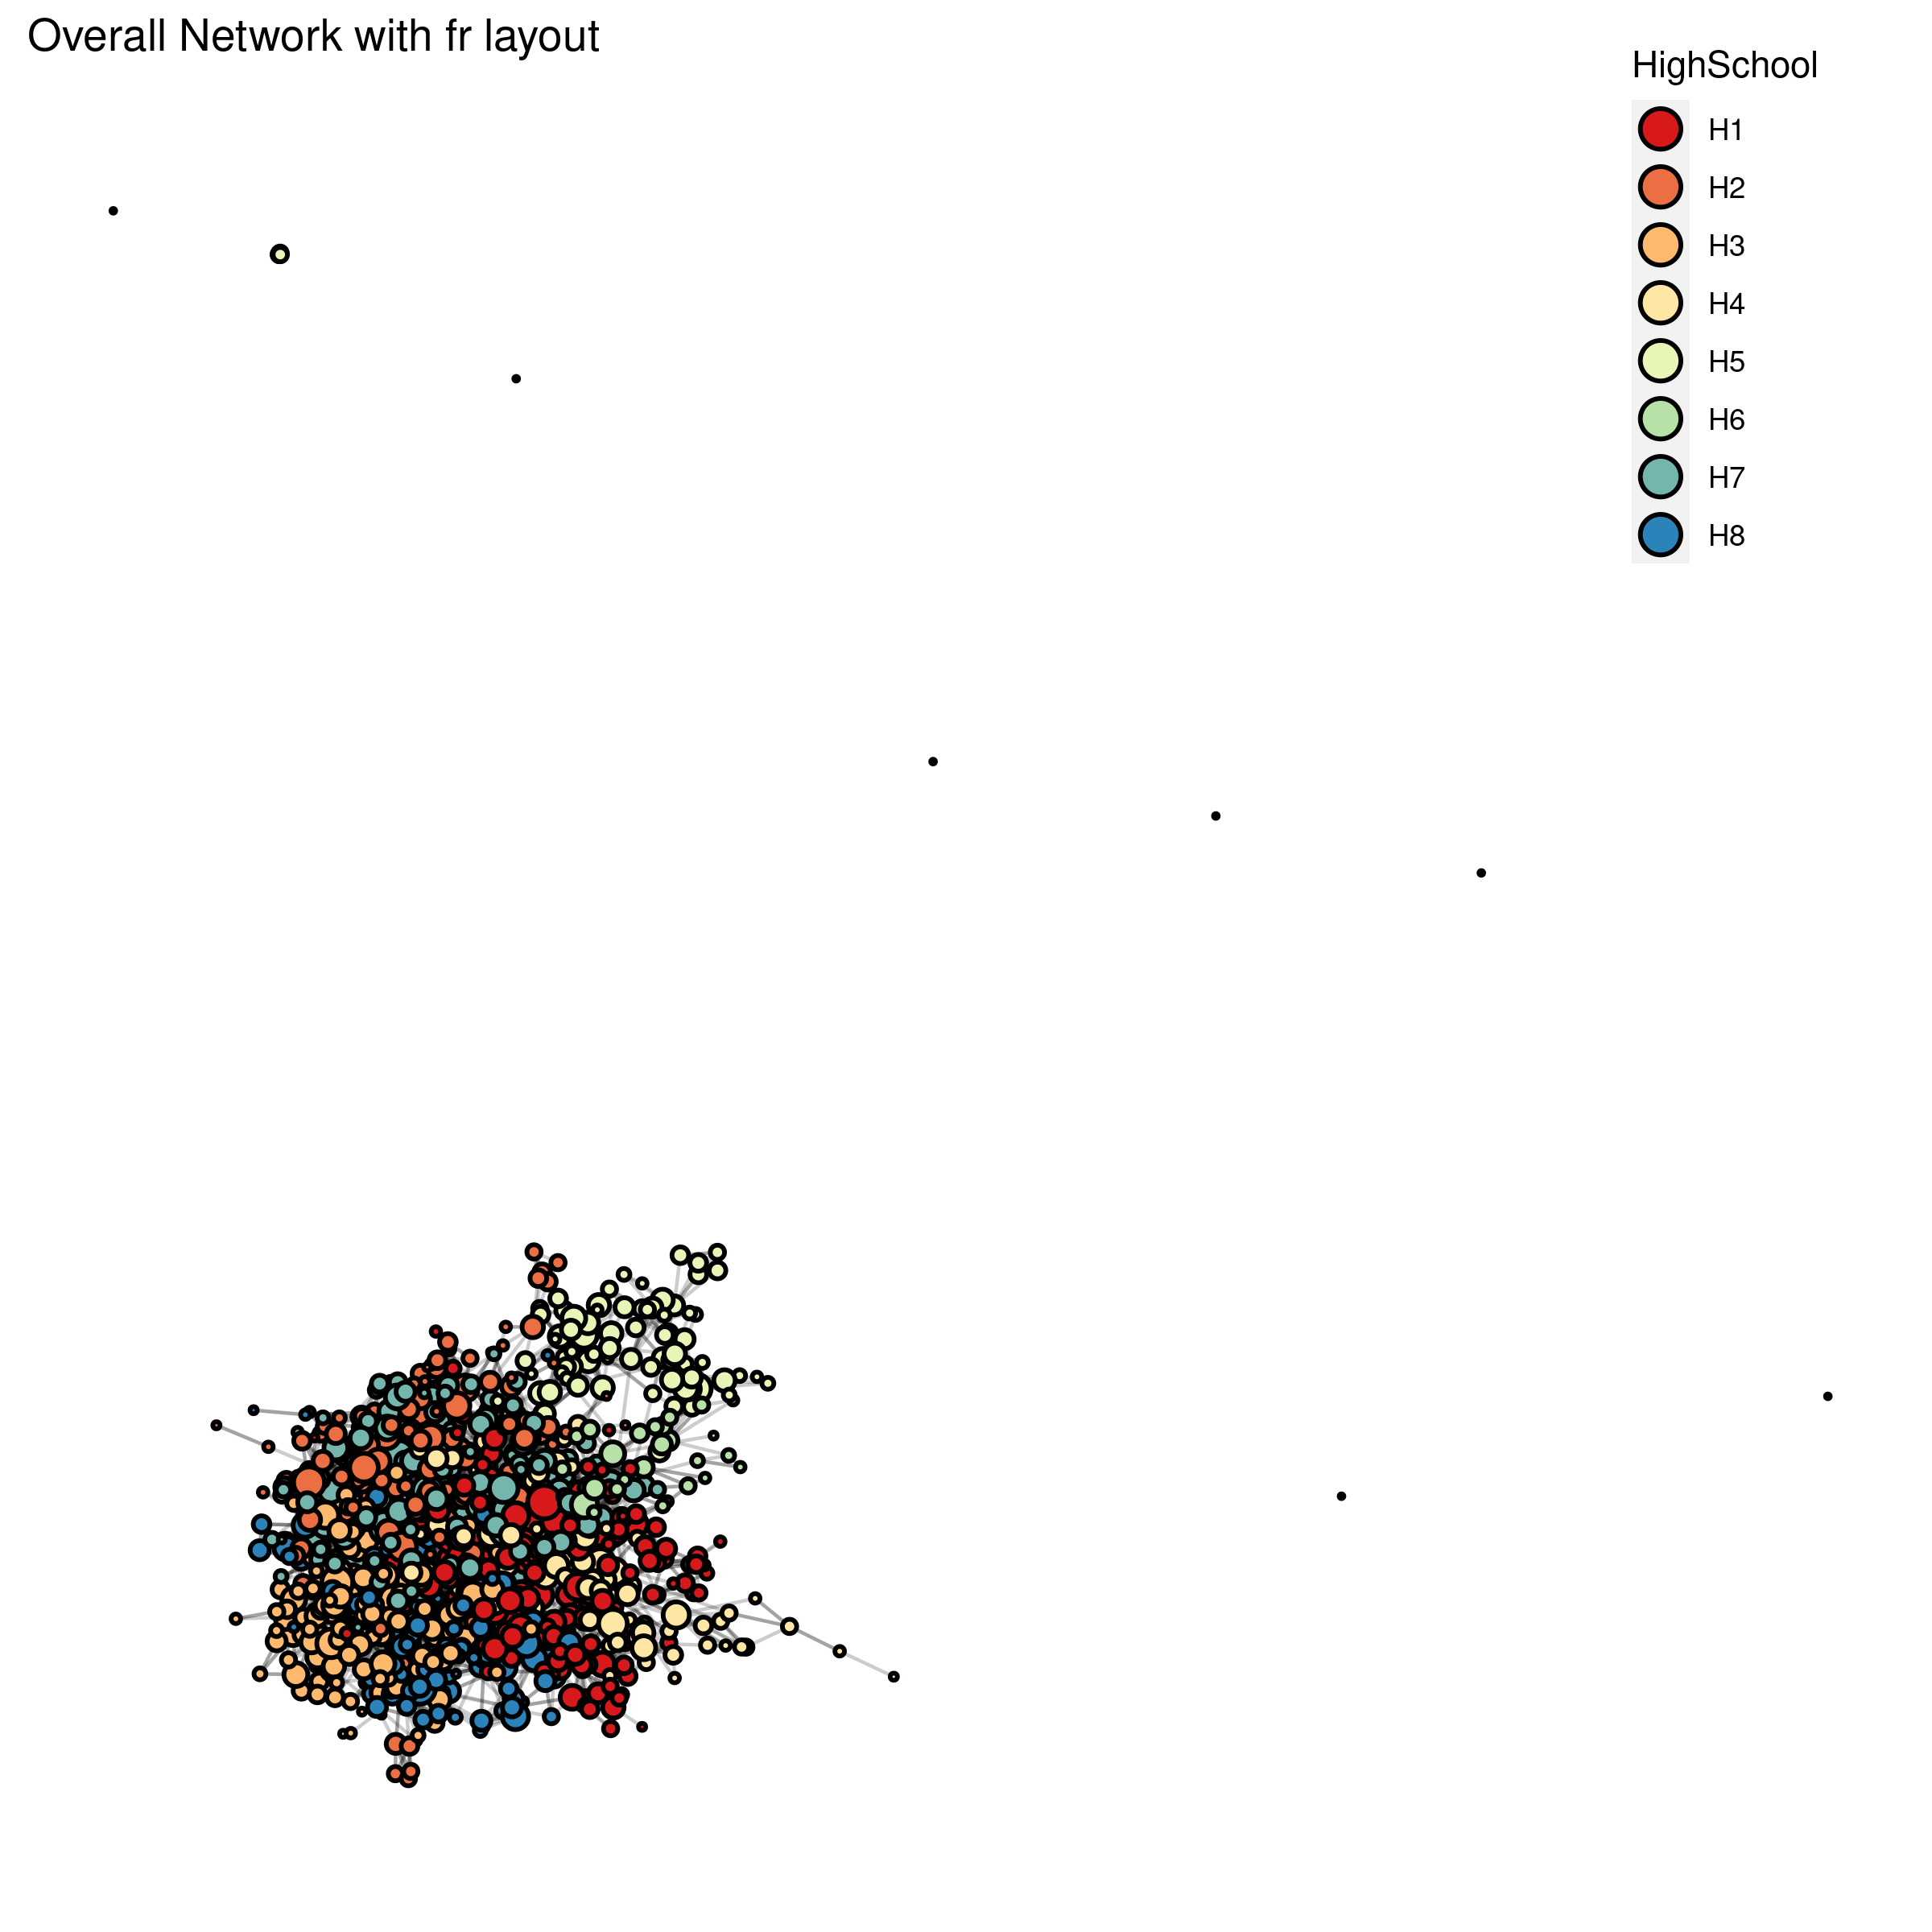
\includegraphics[width=0.7\linewidth]{figures/Networks/Layouts/Graph_OverallNetwork_with_no_highlight_fr_HighSchool___fr.png} 
        \caption{Overall network with a Fruchterman - Reingold algorithm \cite{Fruchterman1991}, it keeps related vertices together. In our case, we have some isolated nodes that are too far away, while the network is clumped in one little space. Also not good.}
        \label{figure:networksLayoutsFR}
    \end{figure}

    \newpage

\subsubsection{Graphopt}

    \begin{figure}[h!]
        \centering
            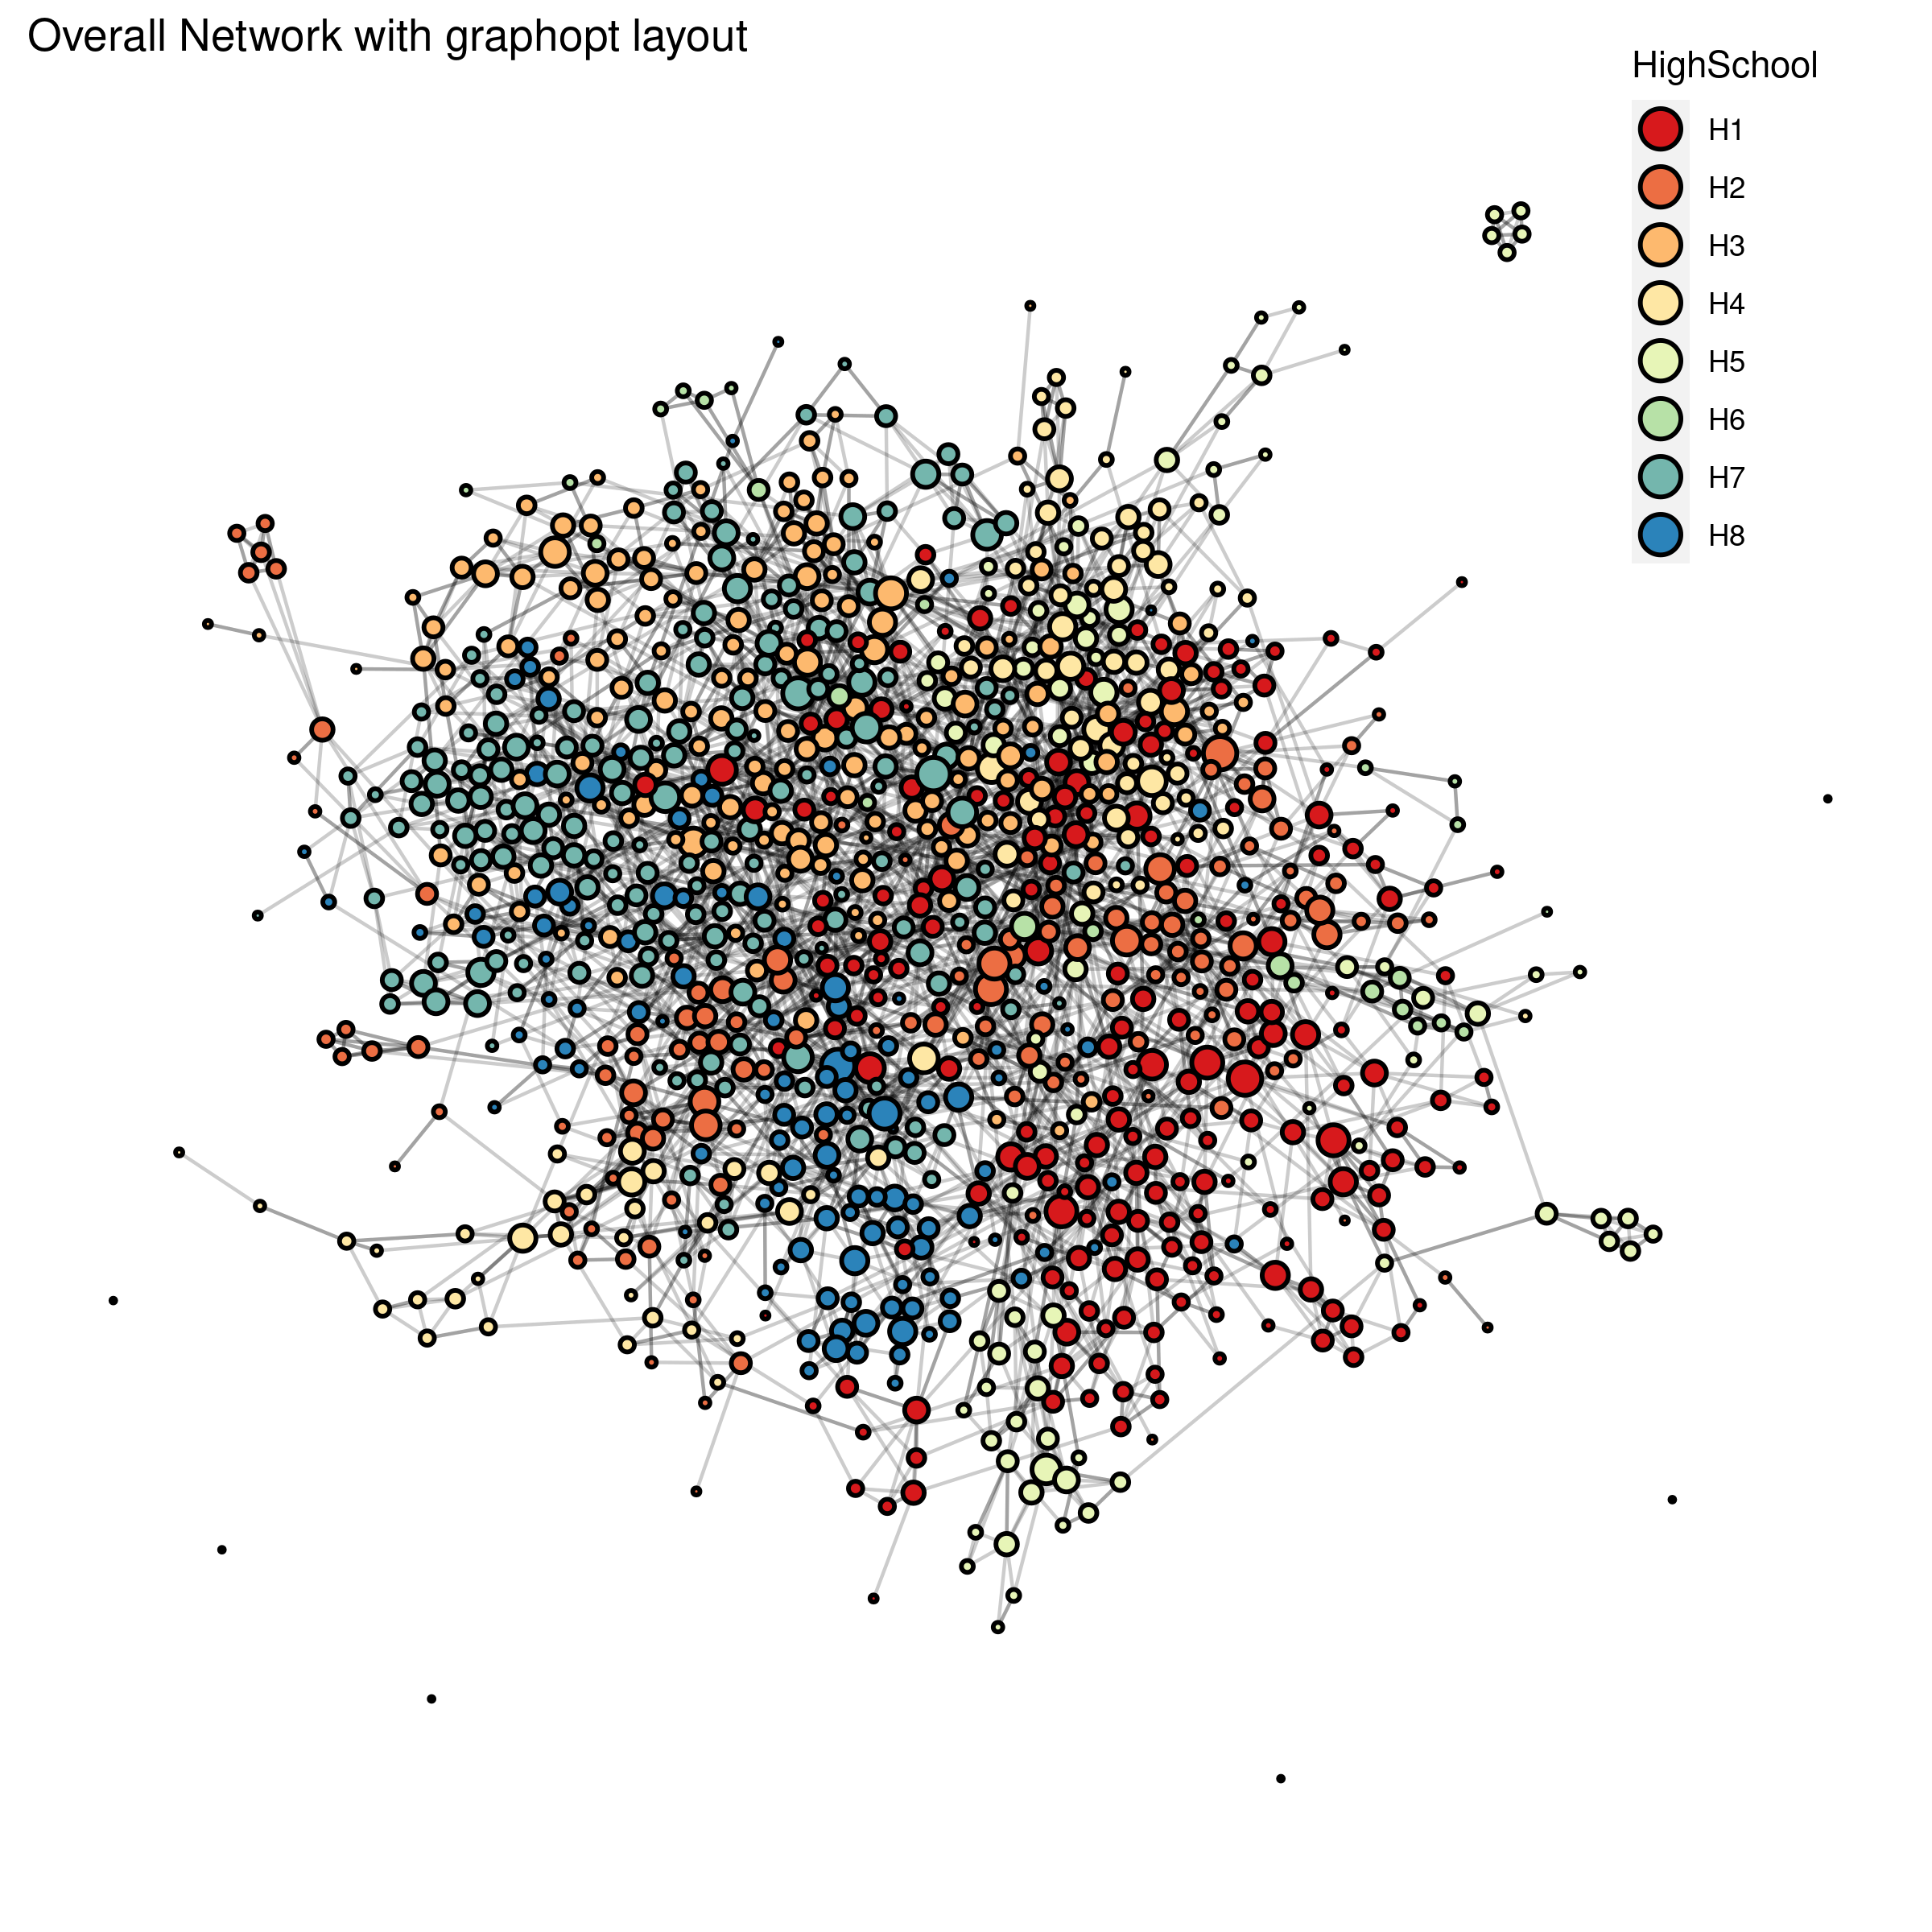
\includegraphics[width=0.7\linewidth]{figures/Networks/Layouts/Graph_OverallNetwork_with_no_highlight_graphopt_HighSchool___graphopt.png} 
        \caption{Overall network with a graphopt layout \cite{gabor2023}. Graphopt (graph optimization) uses physical analogies for defining attracting and repelling forces among the vertices and then the physical system is simulated until it reaches an equilibrium. It aimed to minimize the number of edge crossings to avoid visual cluttering, but in our case, we have too many edges everywhere and an emerging pattern is not clear.}
        \label{figure:networksLayoutsGRAPHOPT}
    \end{figure}

    \newpage

\subsubsection{Kamada-Kawai}

    \begin{figure}[h!]
        \centering
            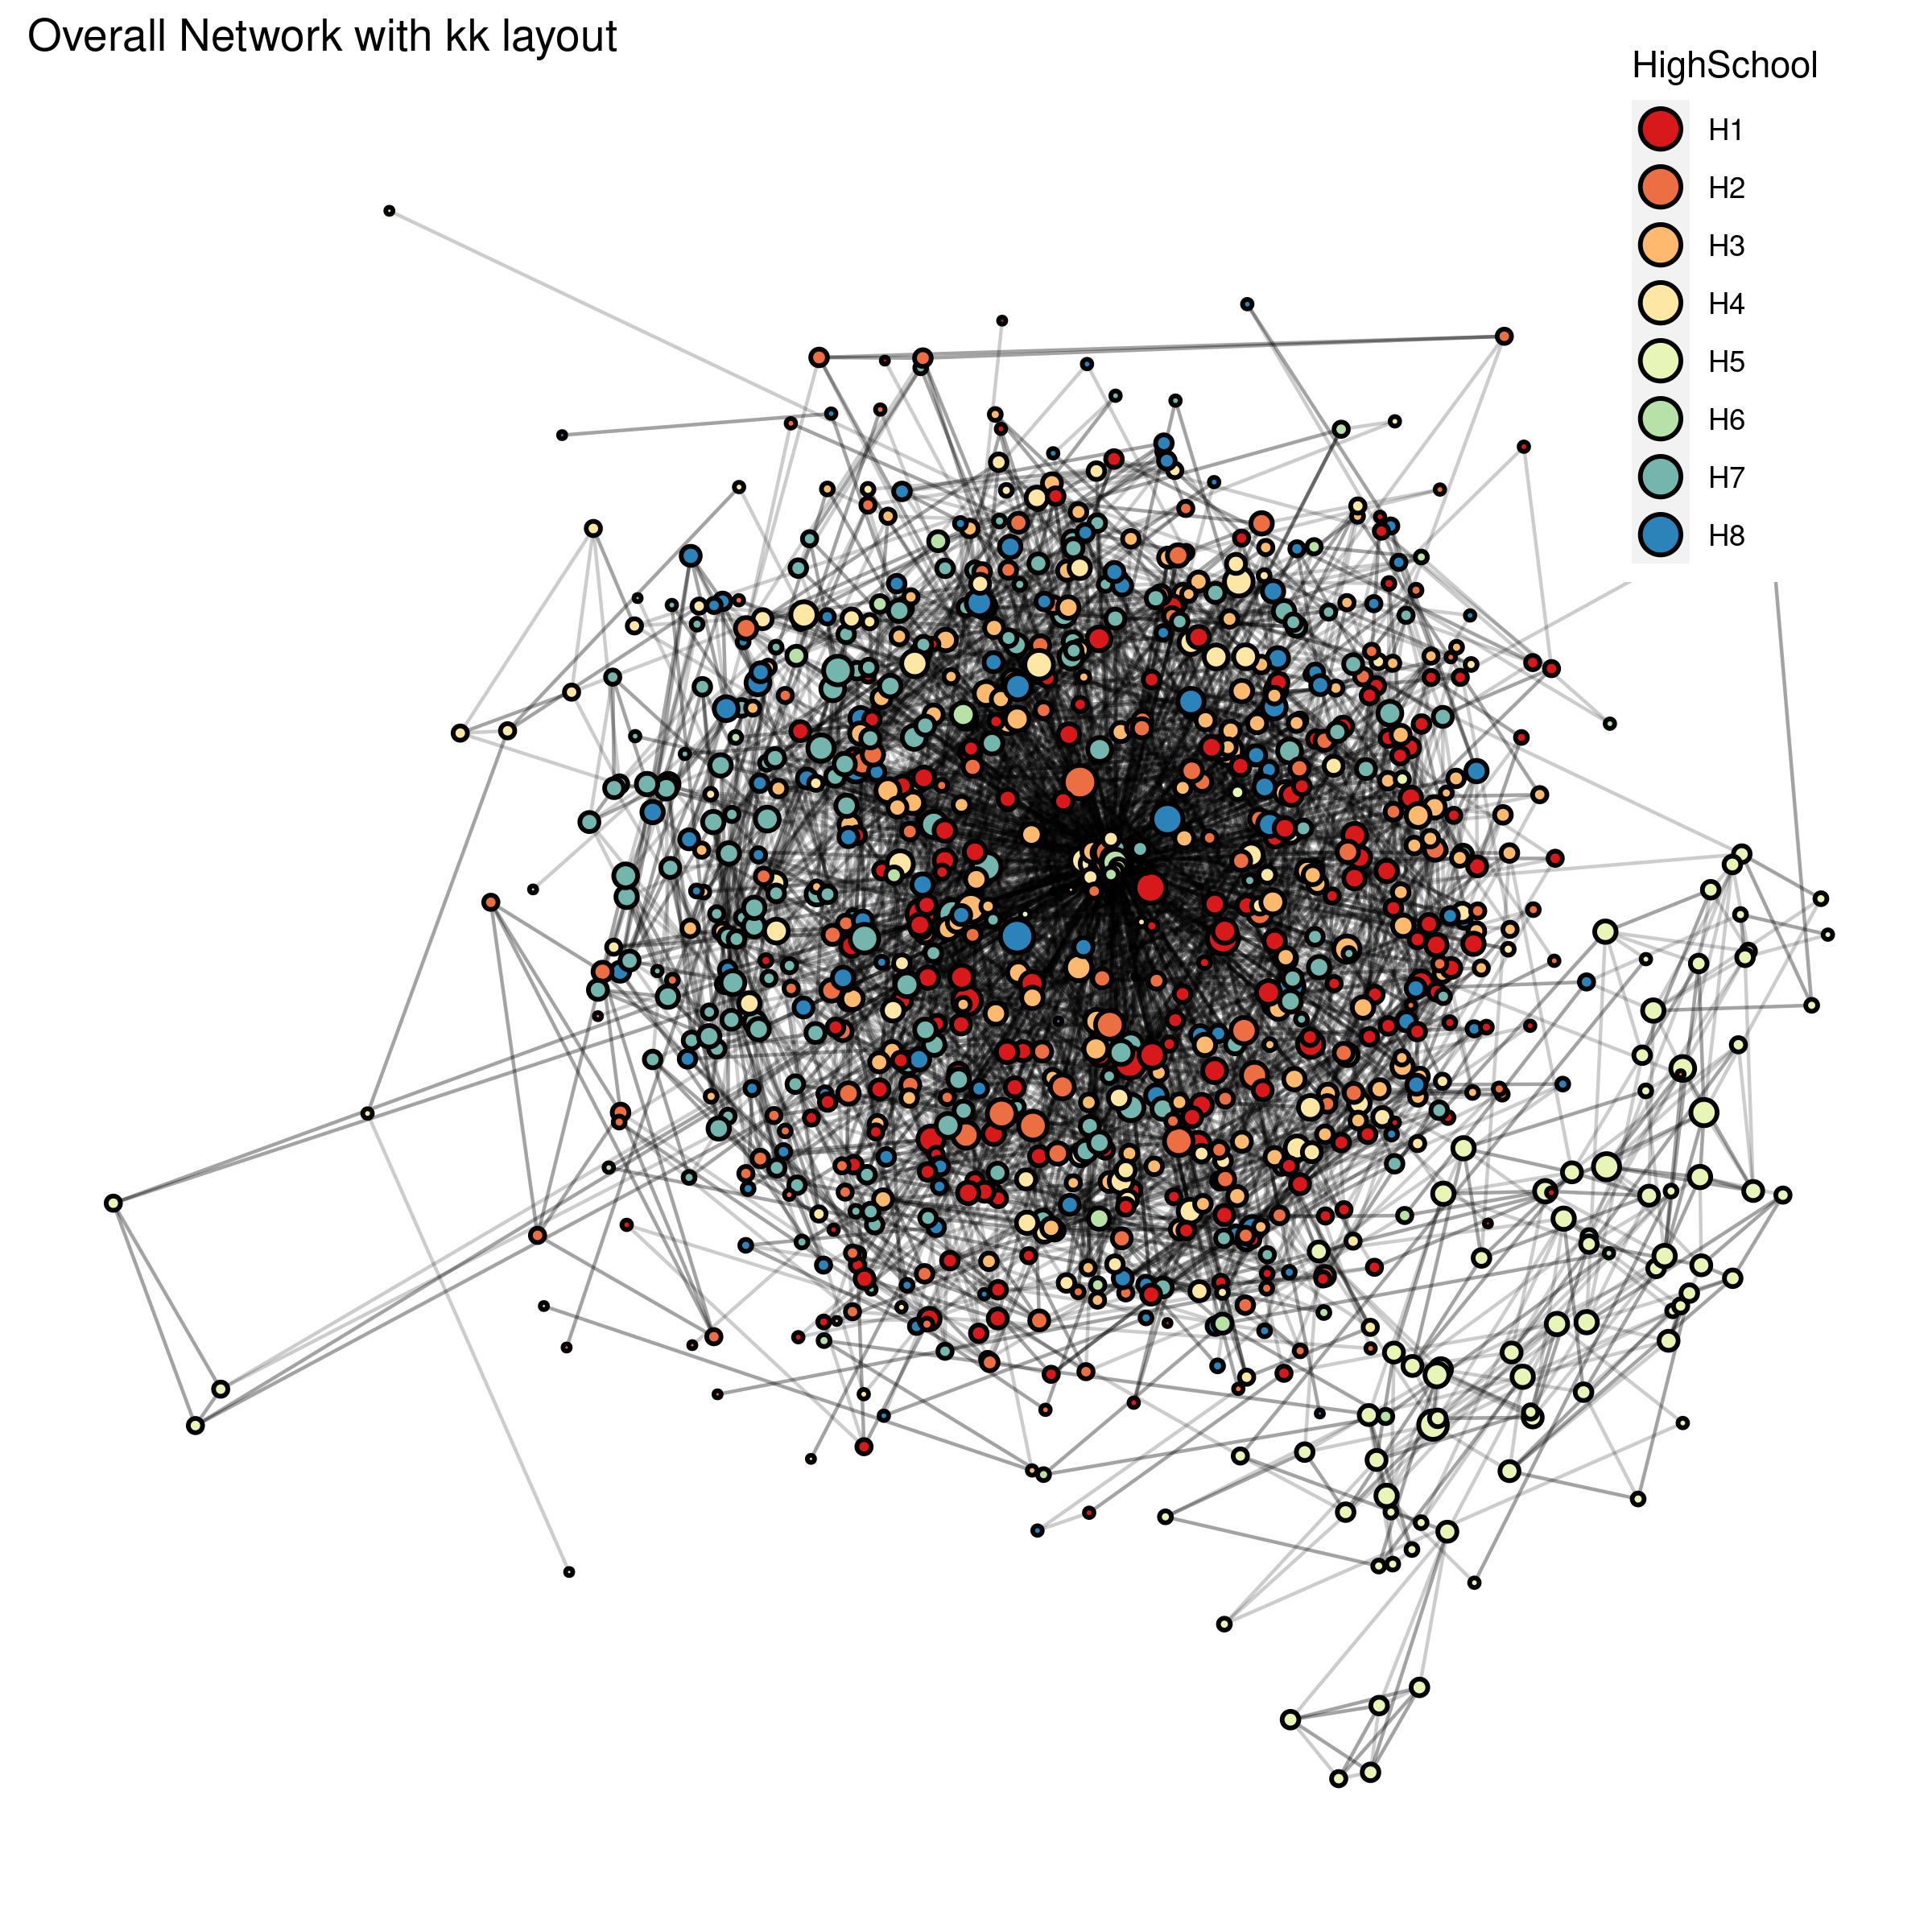
\includegraphics[width=0.7\linewidth]{figures/Networks/Layouts/Graph_OverallNetwork_with_no_highlight_kk_HighSchool___kk.png} 
        \caption{Overall network with a Kamada-Kawai algorithm \cite{Kamada1989}. It put emphasis on the distance as information. Here we see that more isolated nodes are on the outside, and more dense connected areas in the middle. Very useful in other contexts, but again not an ideal choice for us as the core of the network is just a mess of black lines.}
        \label{figure:networksLayoutsKK}
    \end{figure}    

    \newpage

\subsubsection{MDS}

    \begin{figure}[h!]
        \centering
            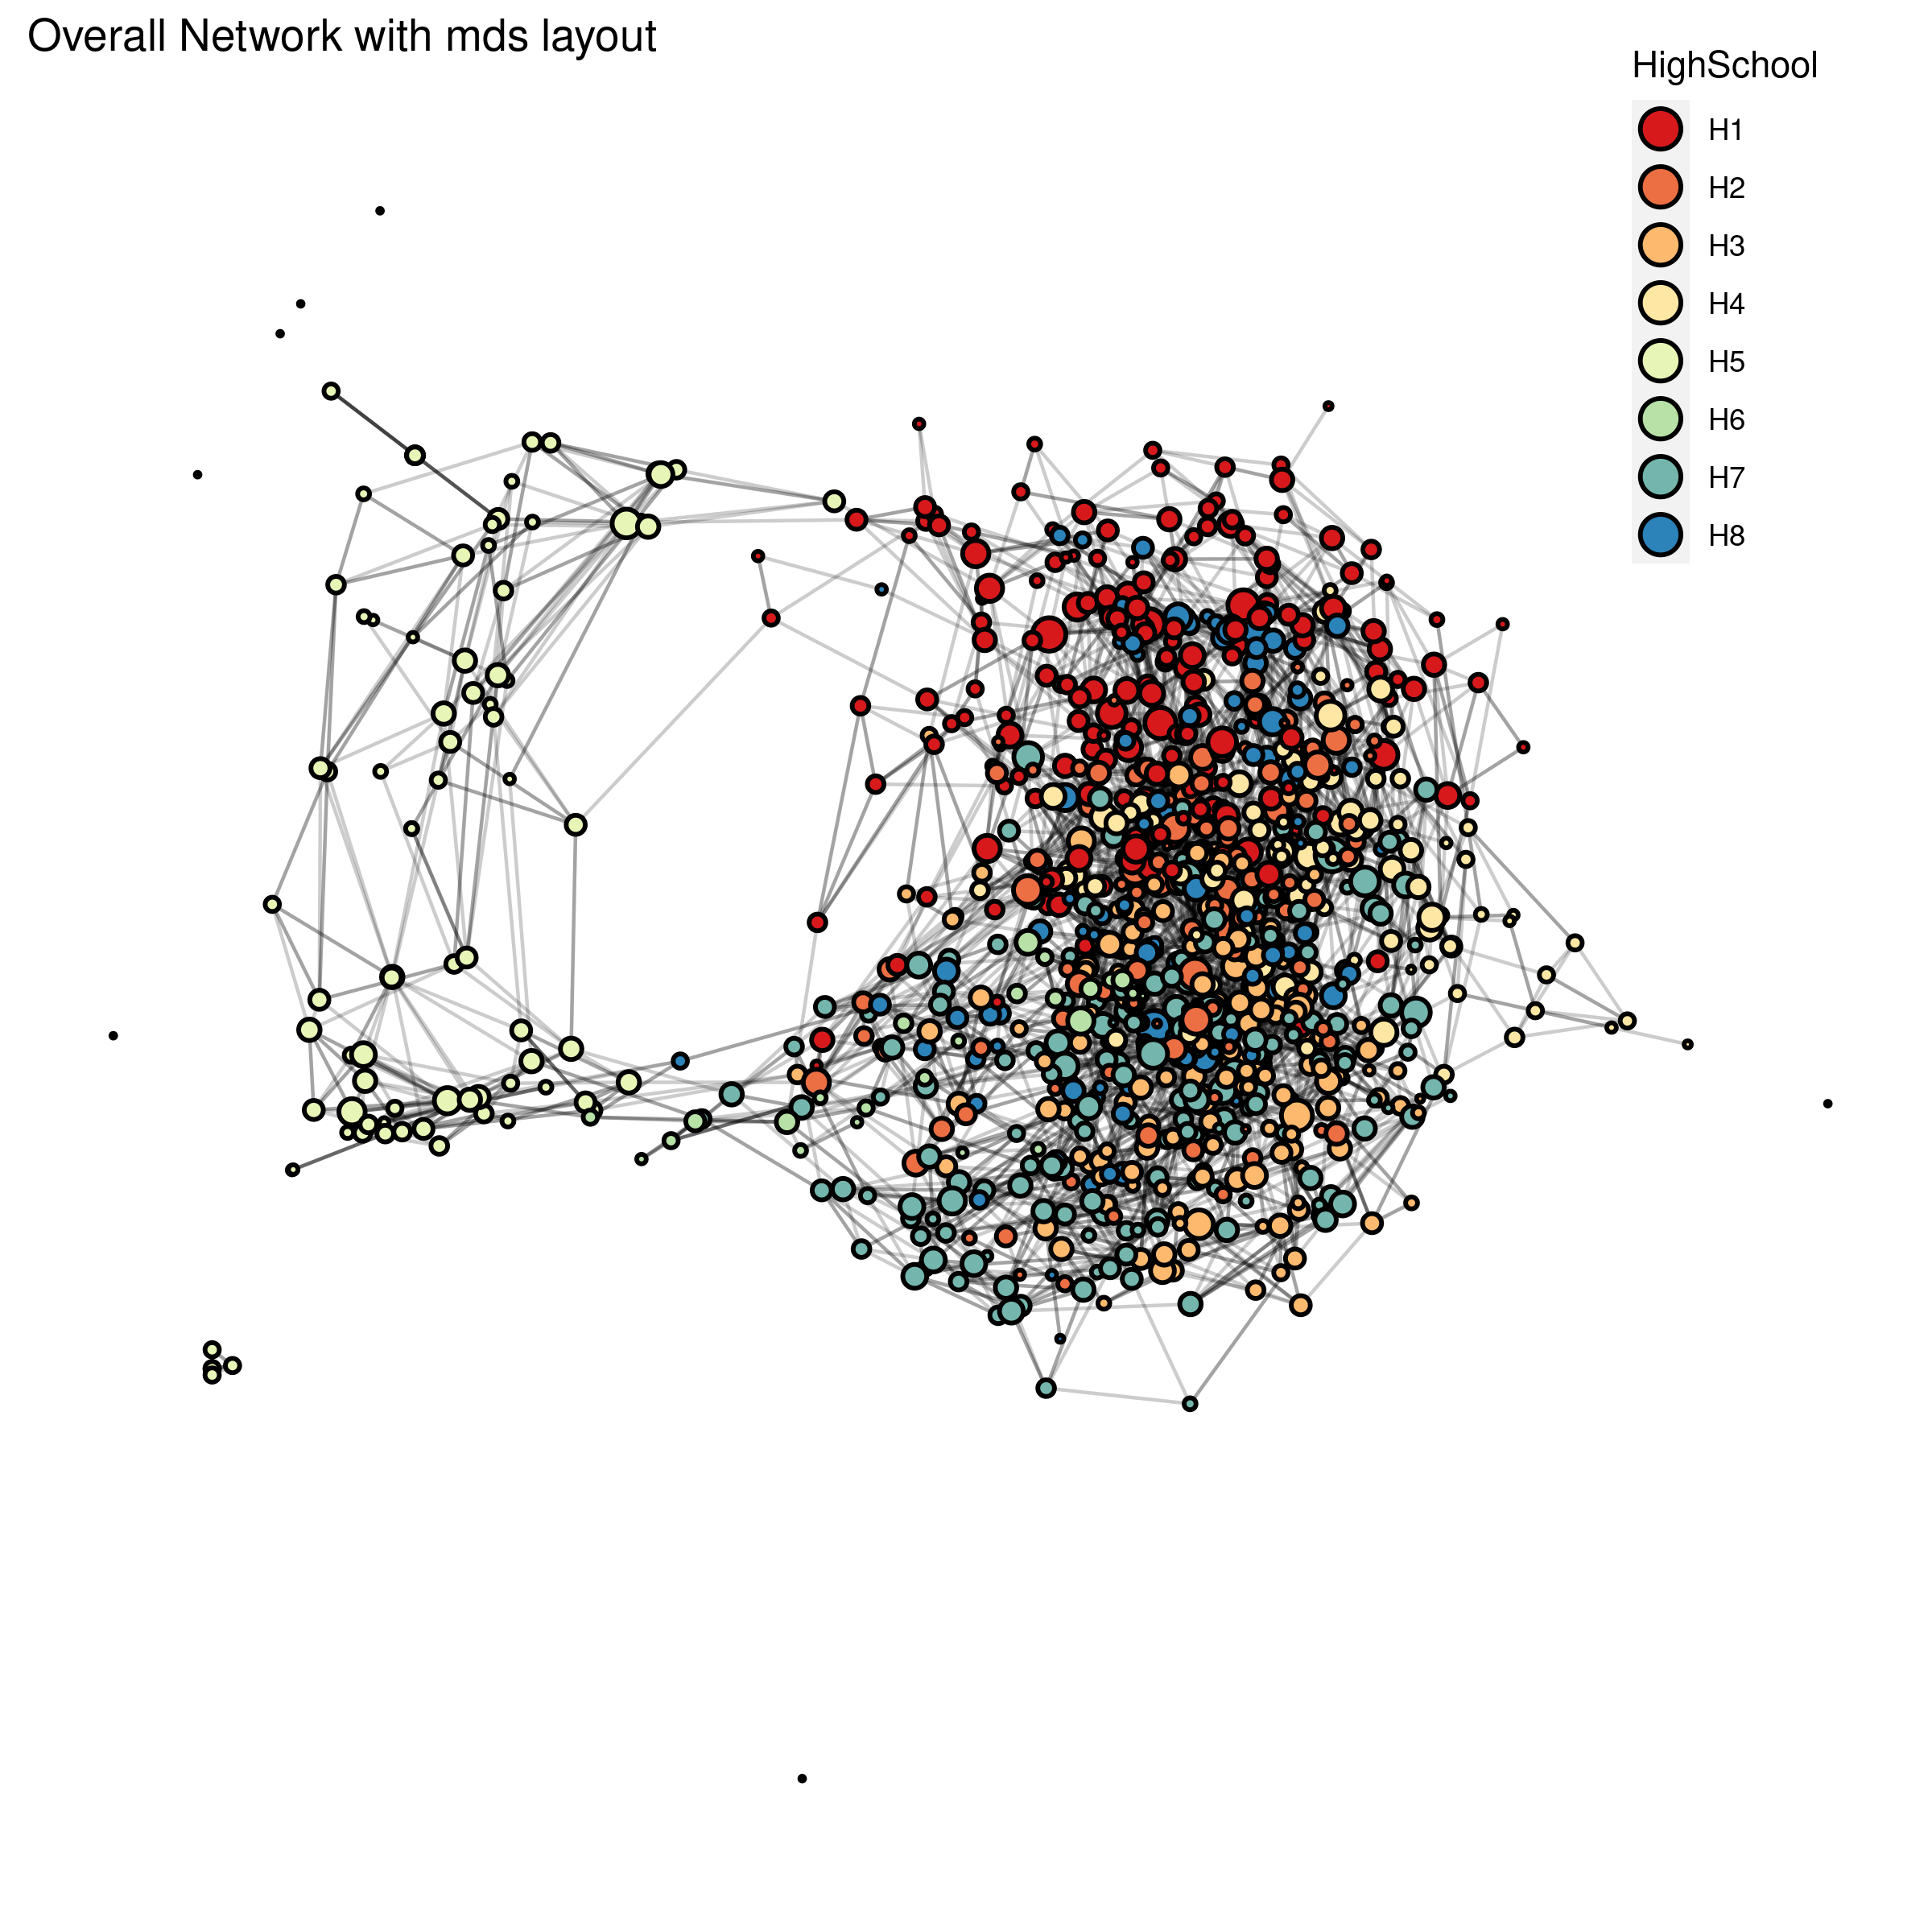
\includegraphics[width=0.7\linewidth]{figures/Networks/Layouts/Graph_OverallNetwork_with_no_highlight_mds_HighSchool___mds.png} 
        \caption{Overall network with \gls{mds} \cite{Buja2008}. When the dissimilarities are distances between high-dimensional objects, MDS acts as a dimension reduction technique. When the dissimilarities are the shortest-path distances in a graph, MDS acts as a graph layout technique. This is our preferred default method because it balances clusters groups of friends together which have some common attributes}
        \label{figure:networksLayoutsMDS}
    \end{figure}    

% MDS Original reference with no DOI http://www.stat.yale.edu/~lc436/papers/JCGS-mds.pdf

    \newpage

\subsubsection{Grouping}

    \begin{figure}[h!]
        \centering
            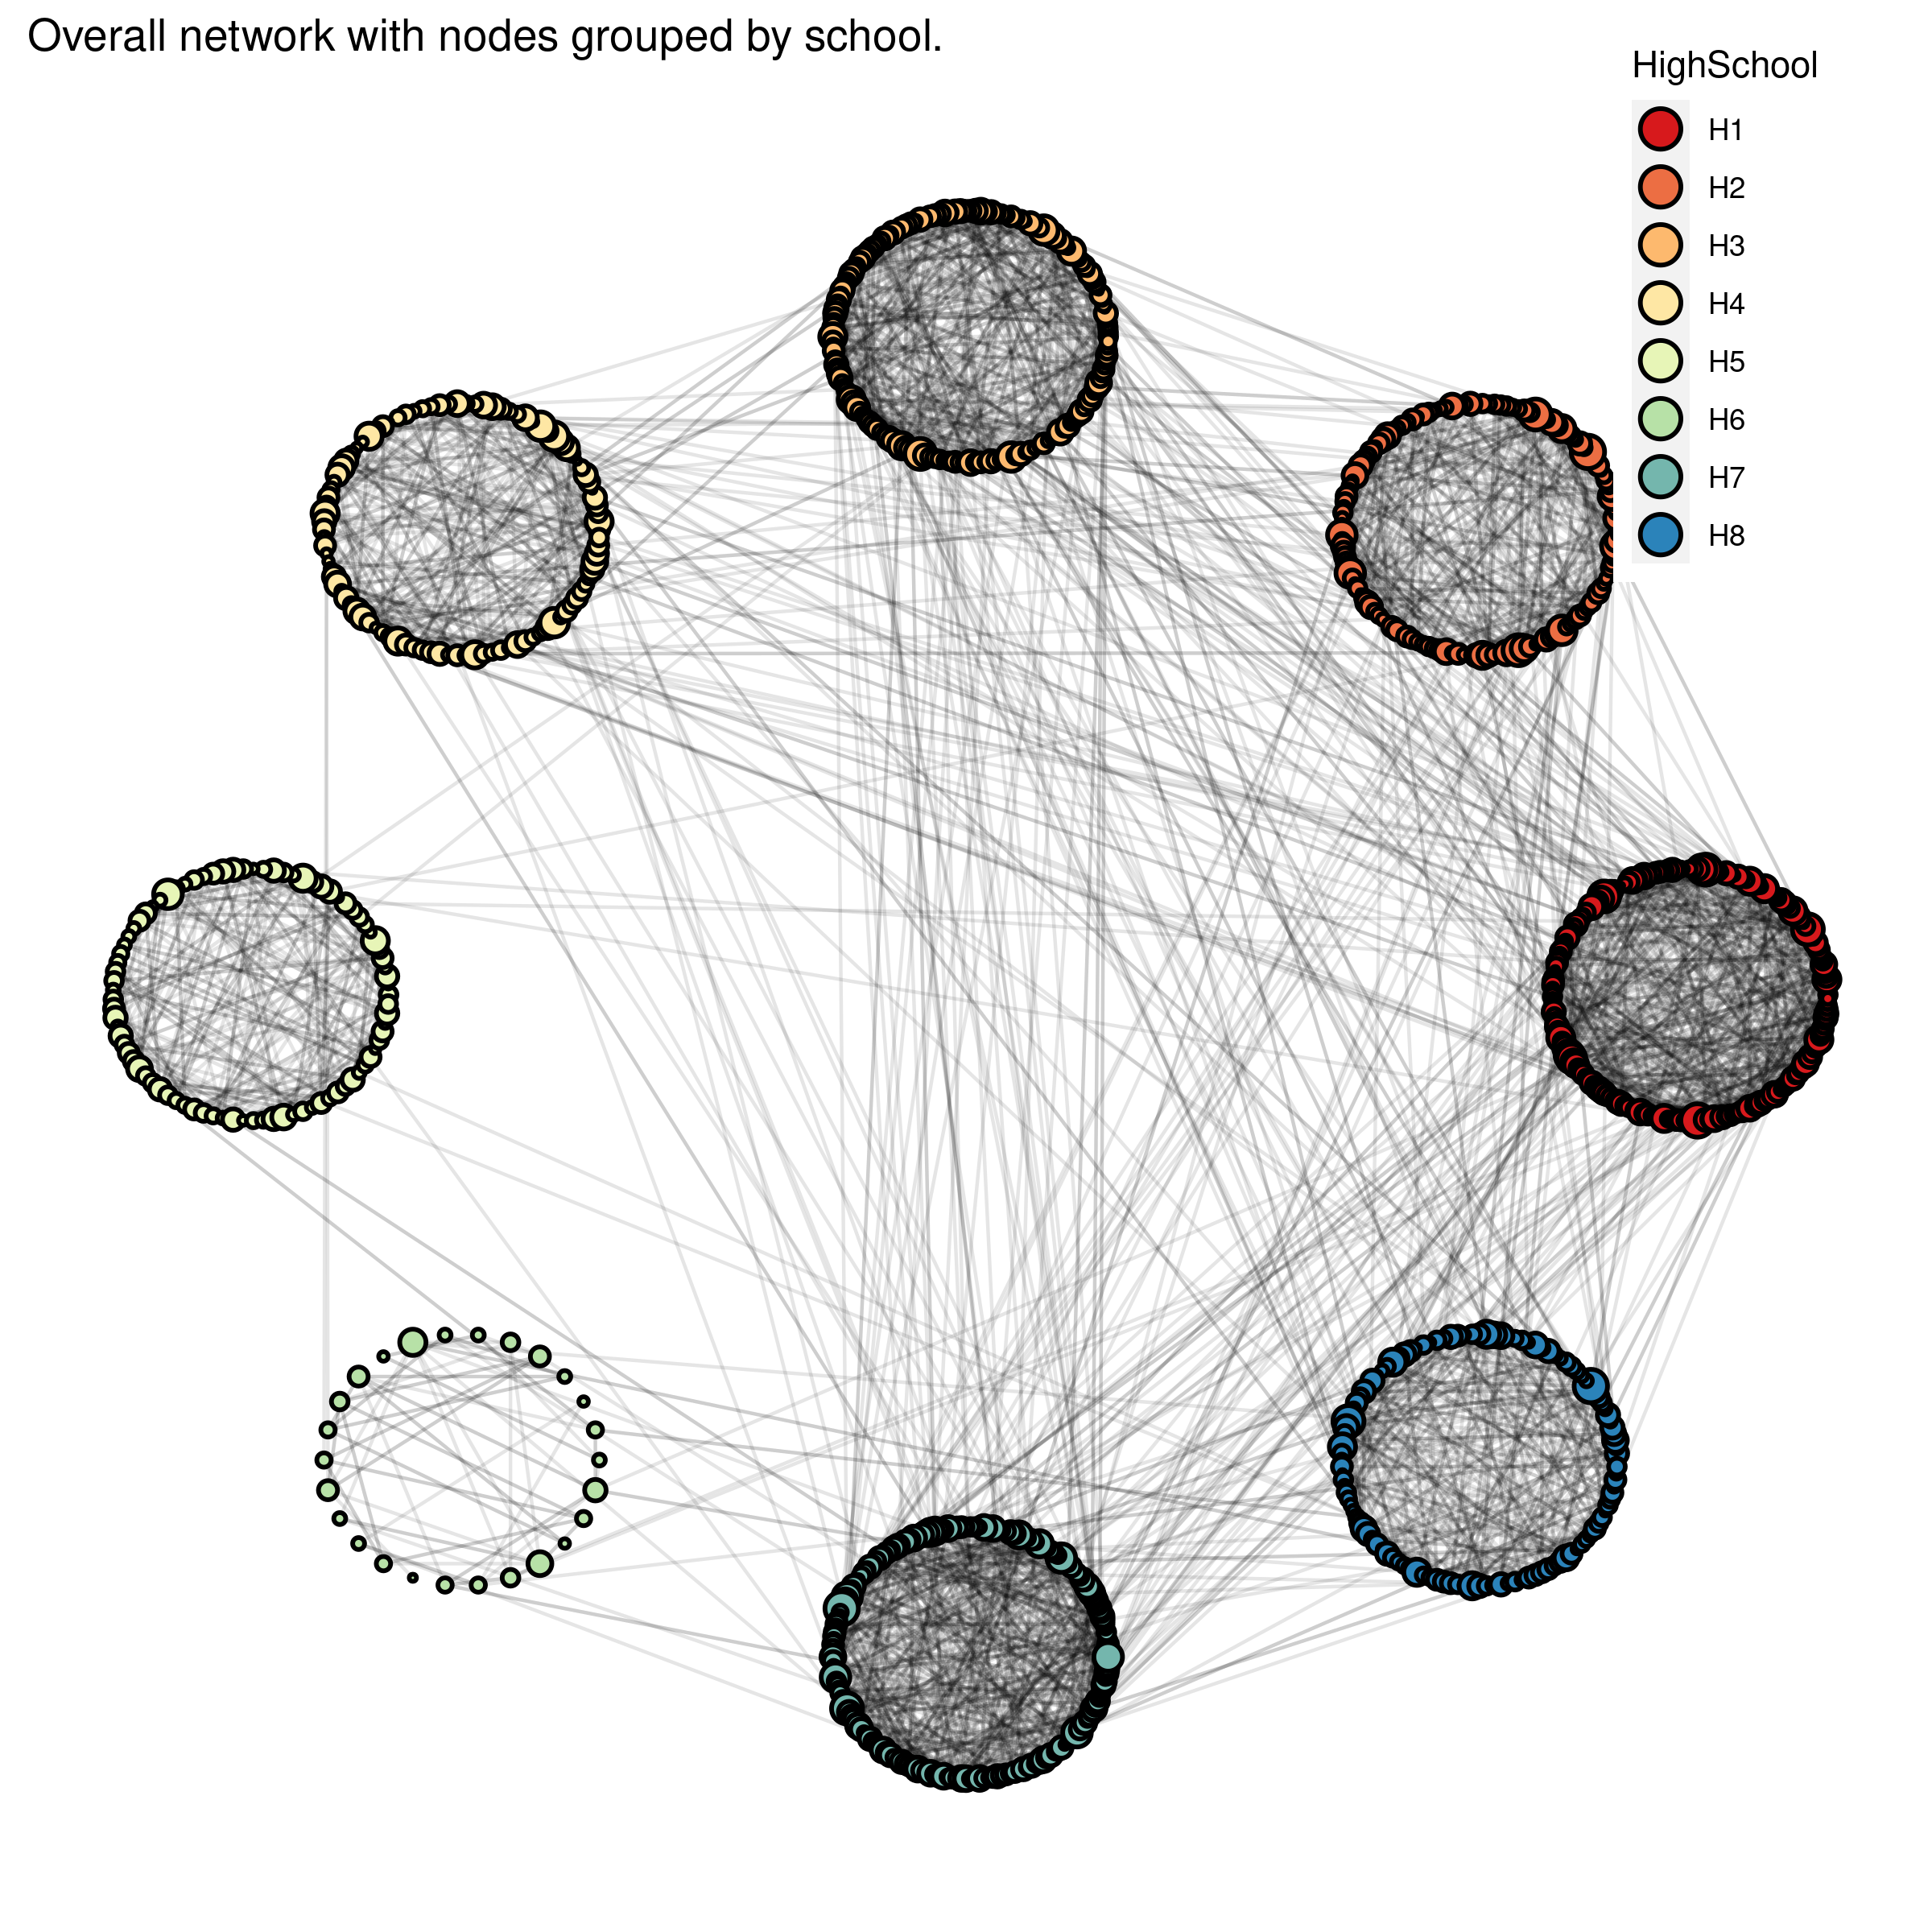
\includegraphics[width=0.7\linewidth]{figures/Networks/Layouts/Graph_OverallNetwork_HS_societal_HighSchool___manual.png} 
        \caption{Overall network sorting nodes into circles, where each circle is a high school. Here is hard to see relationships inside high schools since are densely connected, but ok to see the proportion of relationships between every two pairs of high schools.}
        \label{figure:networksLayoutsMANUAL}
    \end{figure}        

    \newpage

\subsubsection{Geographical}

    \begin{figure}[h!]
        \centering
            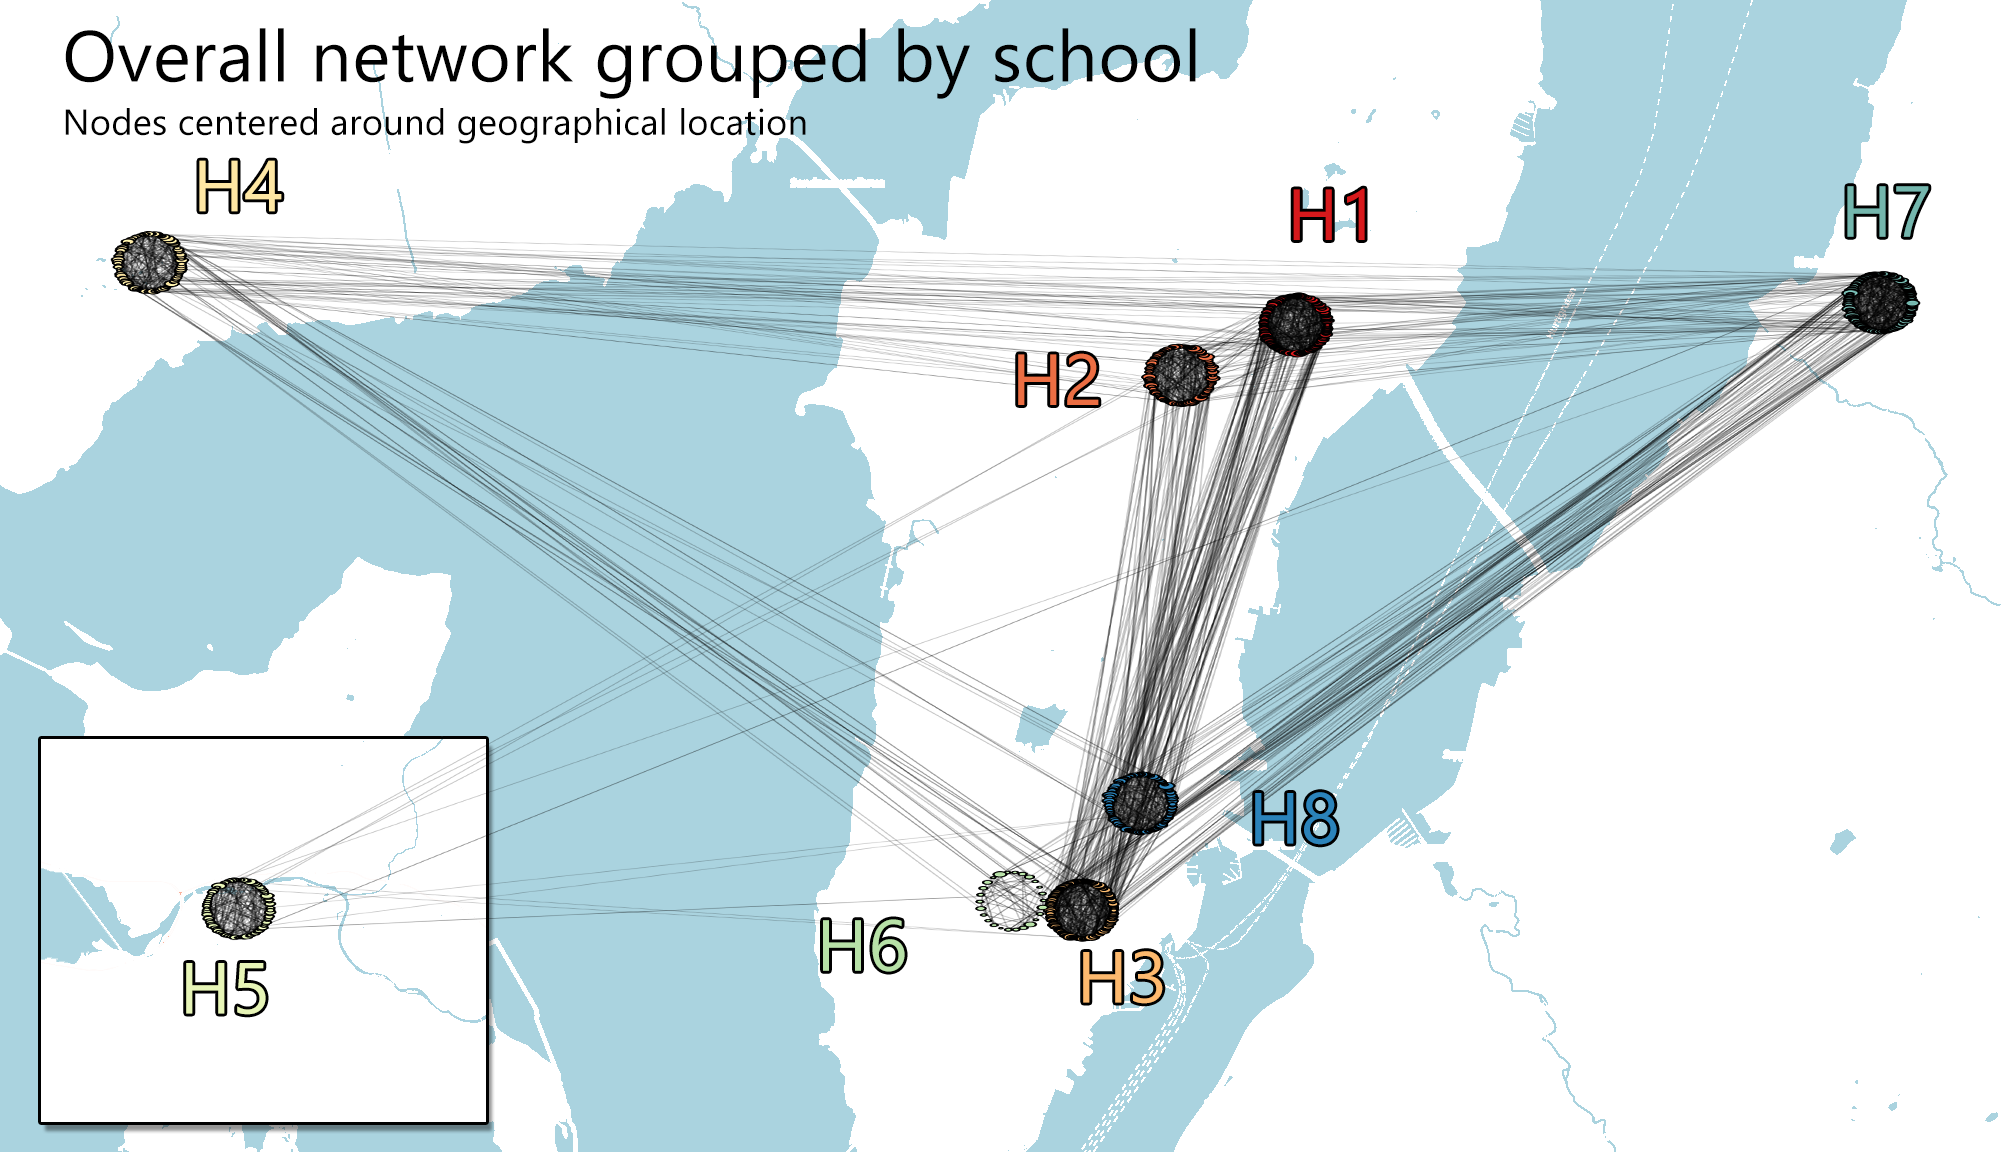
\includegraphics[width=0.9\linewidth]{figures/Networks/Layouts/schoolmapsGraph.png} 
        \caption{Overall network sorting nodes into circles placed according to high-school geographical location. A background outlined map of Tromsø from OpenStreetMaps has been added. Note that H5 is about 120km away from the rest and is brought closer for better visualization.}
        \label{figure:networksLayoutsGEOGRAPHICAL}
    \end{figure}        

    \newpage

\section{Networks metrics}

\subsection{How important is a node in a network?}

% Centralities, correct terminology! https://eehh-stanford.github.io/SNA-workshop/graphs.html#dyads-triads-and-other-local-structures

Nodes are not only important because they have many connections as we saw in section \ref{network:Connectivity}. The following metrics can help you identify nodes in the network that might also be relevant. But none of them is a better or worse method, it depends on what you consider to be important in your context:

\subsubsection{Degree centrality}

The most obvious one is to measure the number of connections \cite{Freeman1978}. In social networks, well-connected nodes are people with high popularity, which tends to be indicative of importance. In medical interventions, we like to target high connectivity nodes to become healthy because they tend to influence their peers to become healthy as well. In figure \ref{figure:networksLayoutsMDS} we can see the network with the node size proportional to the number of connections each student has.

\subsubsection{Closeness centrality}

In this context, we measure the importance of the nodes proportionally to their path with any other given node \cite{Freeman1978}. The idea is that an important node is one that is capable of reaching other nodes very quickly. The importance of this is more obvious in topology networks with weighted edges, where a town can be well connected to other towns, but using semi-destroyed and badly maintained roads, making it a less attractive node to put a central hub. In comparison, a town that is less connected but with a newly built 4 lanes highway, might be a better option. When a closeness centrality number is high, it means that the node is central in the network and is close to other nodes in the network. This indicates that the node has better accessibility to other nodes and can easily reach these nodes. An example of this metric can be seen in figure \ref{figure:networksCloseness}.

    \begin{figure}[h!]
        \centering
            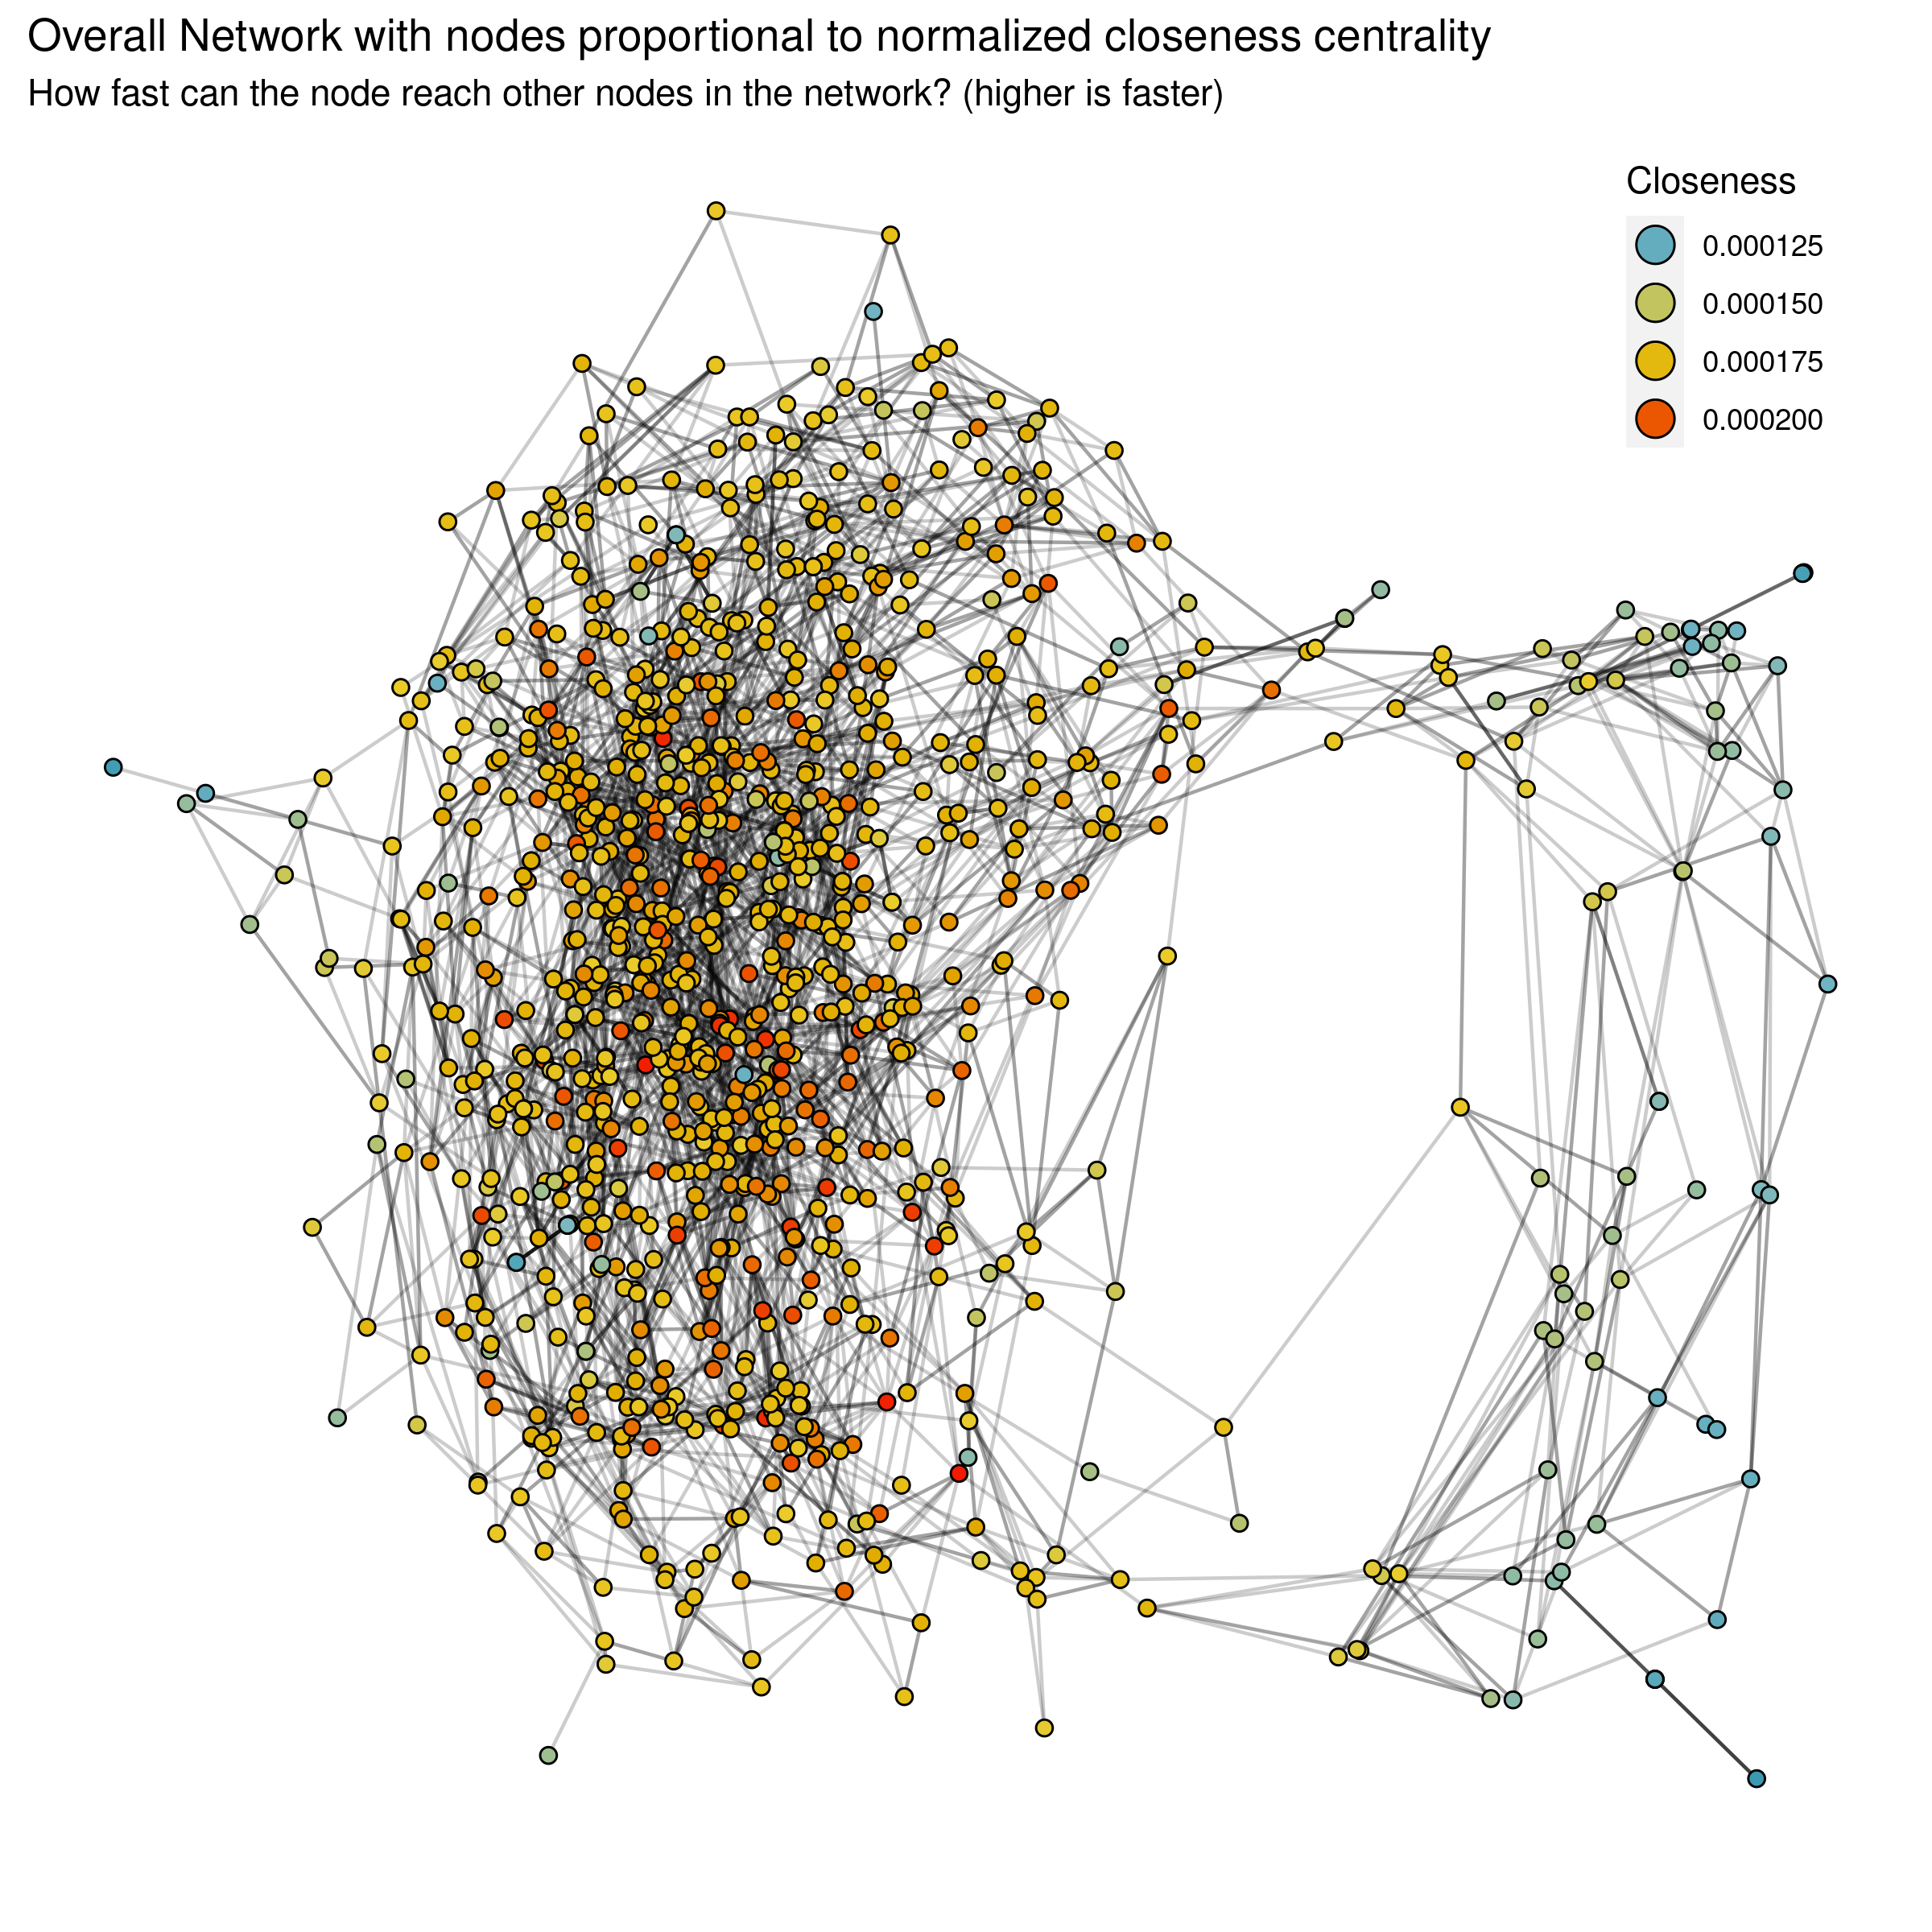
\includegraphics[width=0.9\linewidth]{figures/Networks/Centralities/Graph_temporalEdgesDF_centralitiesDF_Closeness___mds.png} 
        \caption{Overall network coloring nodes by their closeness. Disconnected nodes and subnetworks have outlier values and have been removed for better color scale}
        \label{figure:networksCloseness}
    \end{figure}      

\subsubsection{Betweenness centrality}

Central nodes are nodes that connect several subnetworks together \cite{Freeman1978}. In epidemiology identifying these nodes are critical because we can stop the progress of the disease by targeting these nodes alone, and thus isolating each of the individual clusters. An example of this metric can be seen in figure \ref{figure:networksBetweenness}.

    \begin{figure}[h!]
        \centering
            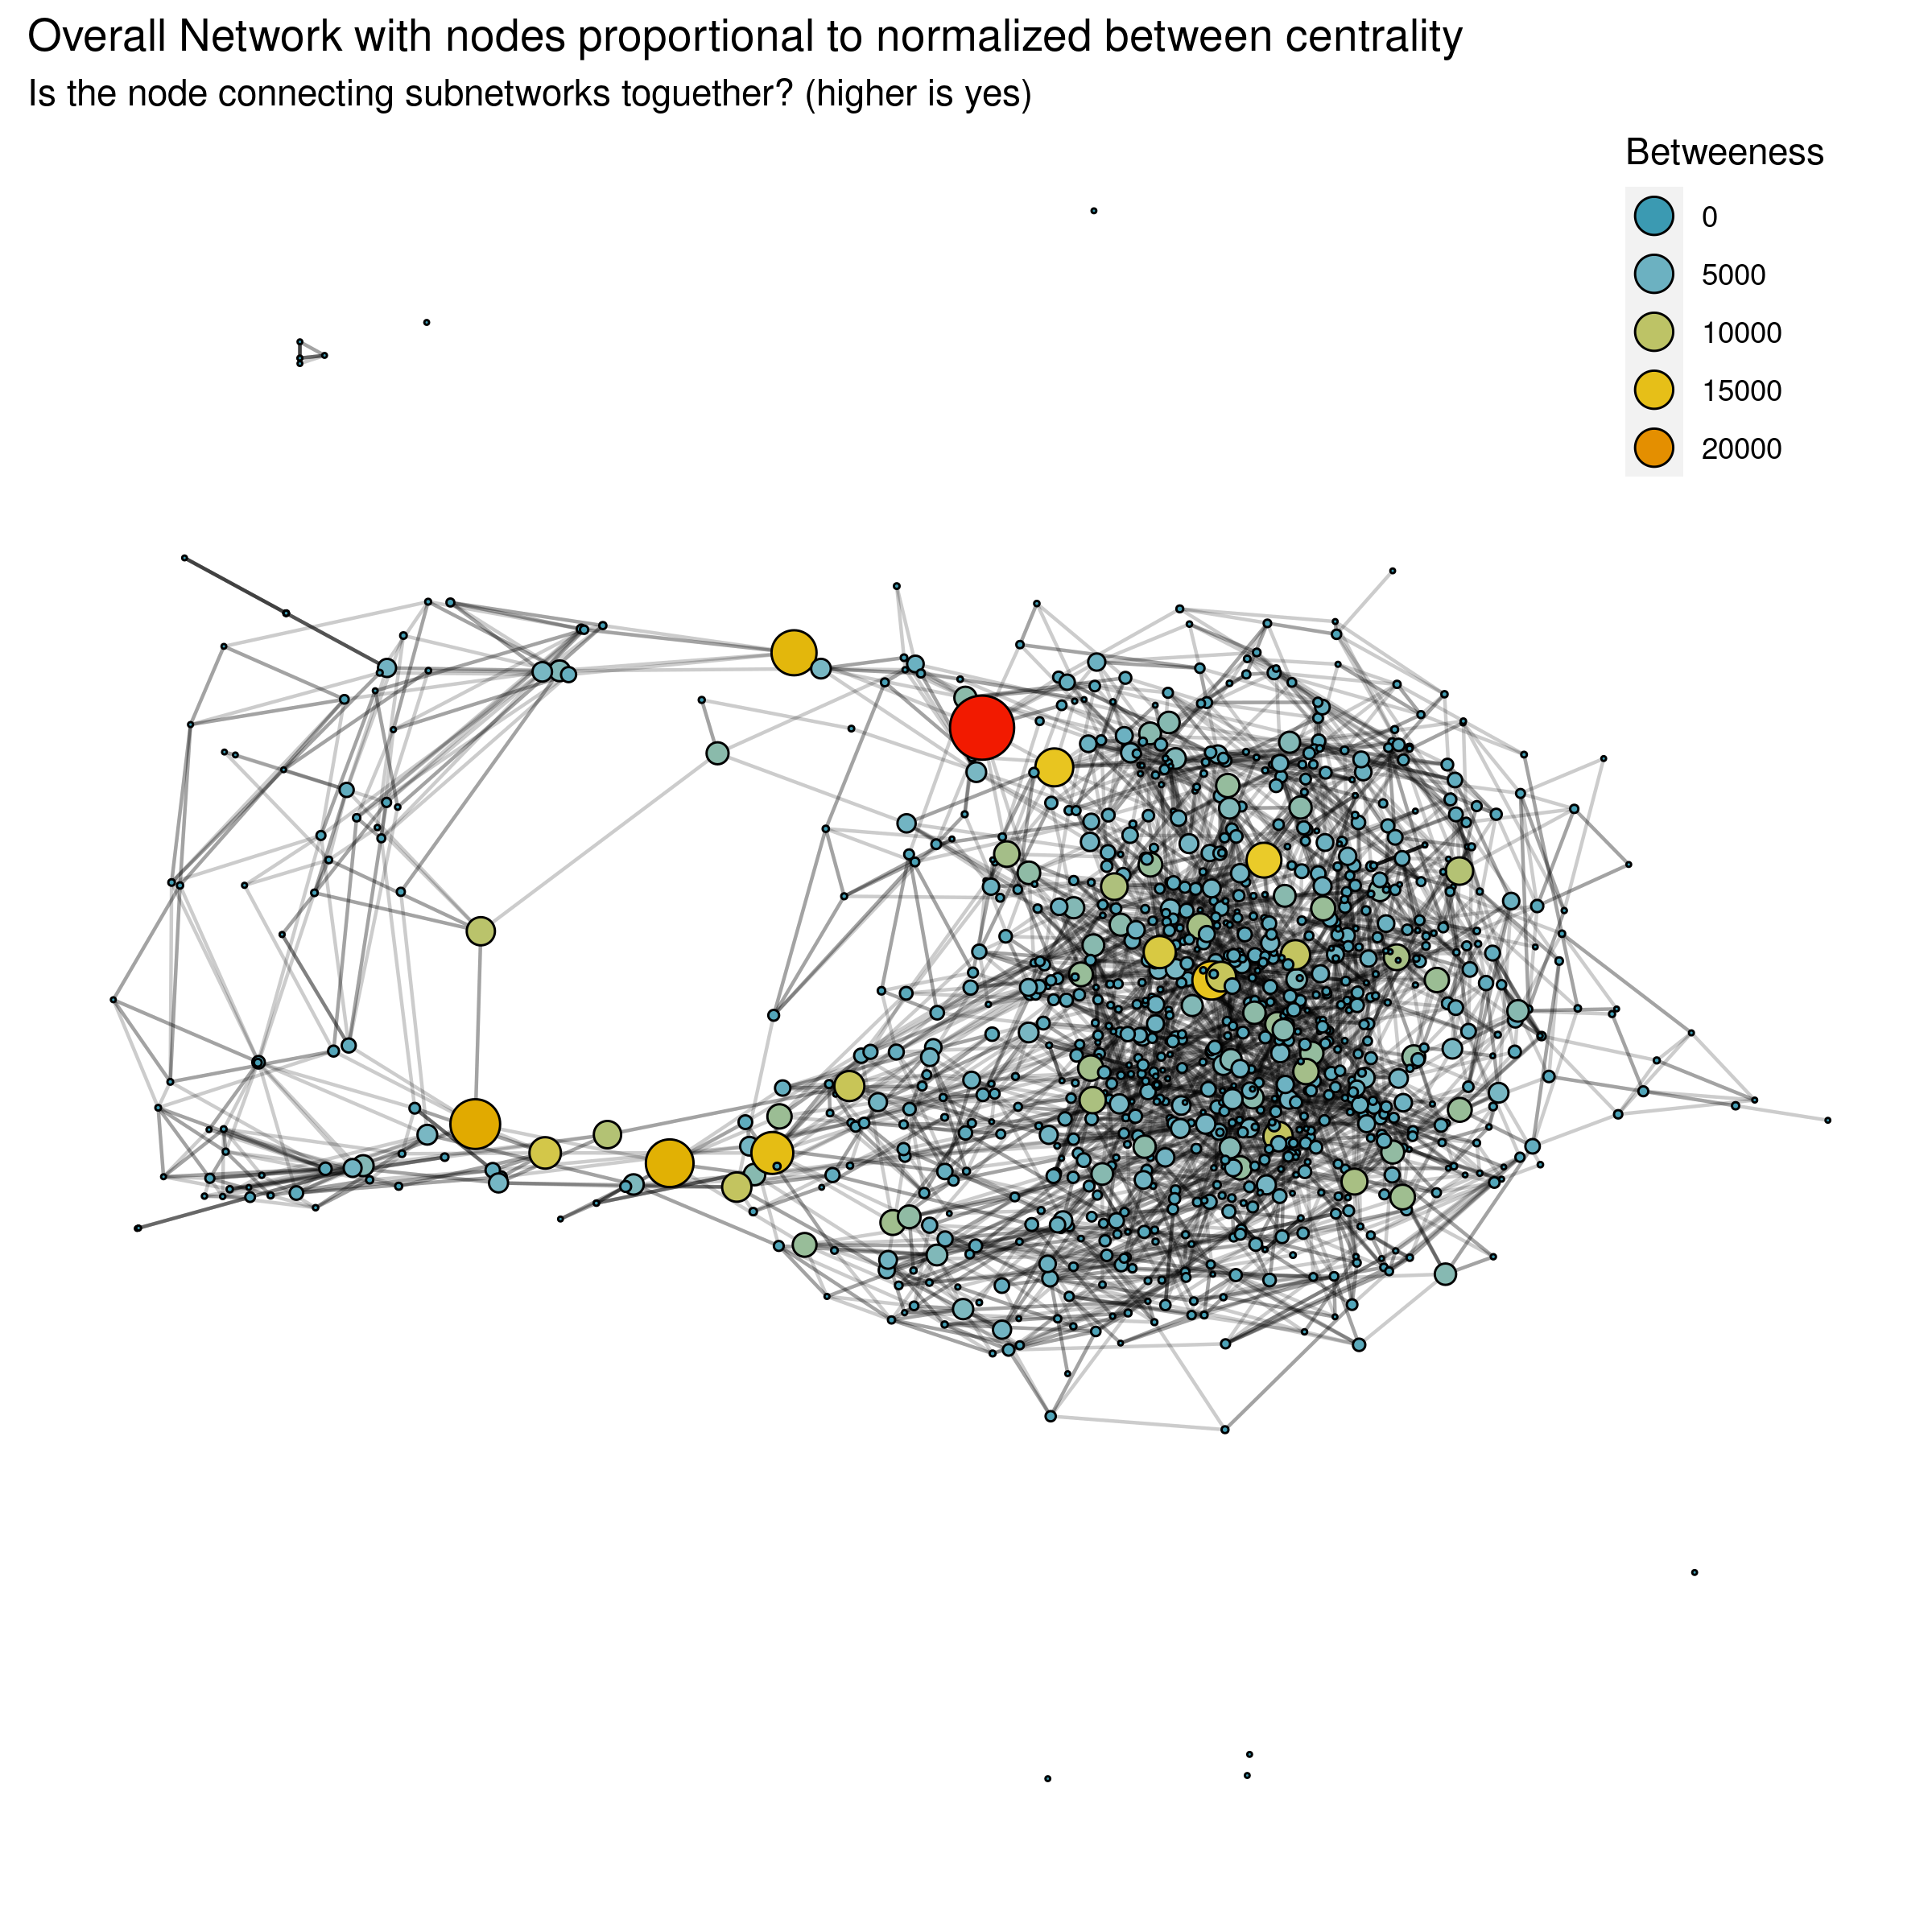
\includegraphics[width=0.9\linewidth]{figures/Networks/Centralities/Graph_overallEdgesDF_centralitiesDF_Betweeness___mds.png} 
        \caption{Overall network coloring nodes by their betweenness. Node size is proportional to betweenness.}
        \label{figure:networksBetweenness}
    \end{figure}      

\subsubsection{Eigencentrality}

When you don't care about the number of connections, but about the quality of the connections, then eigencentrality is what is used to measure the important nodes \cite{Bonacich1972}. In general, vertices with high eigenvector centralities are those which are connected to many other vertices which are, in turn, connected to many others, and so on. An example of this metric can be seen in figure \ref{figure:networksEigen}.

    \begin{figure}[h!]
        \centering
            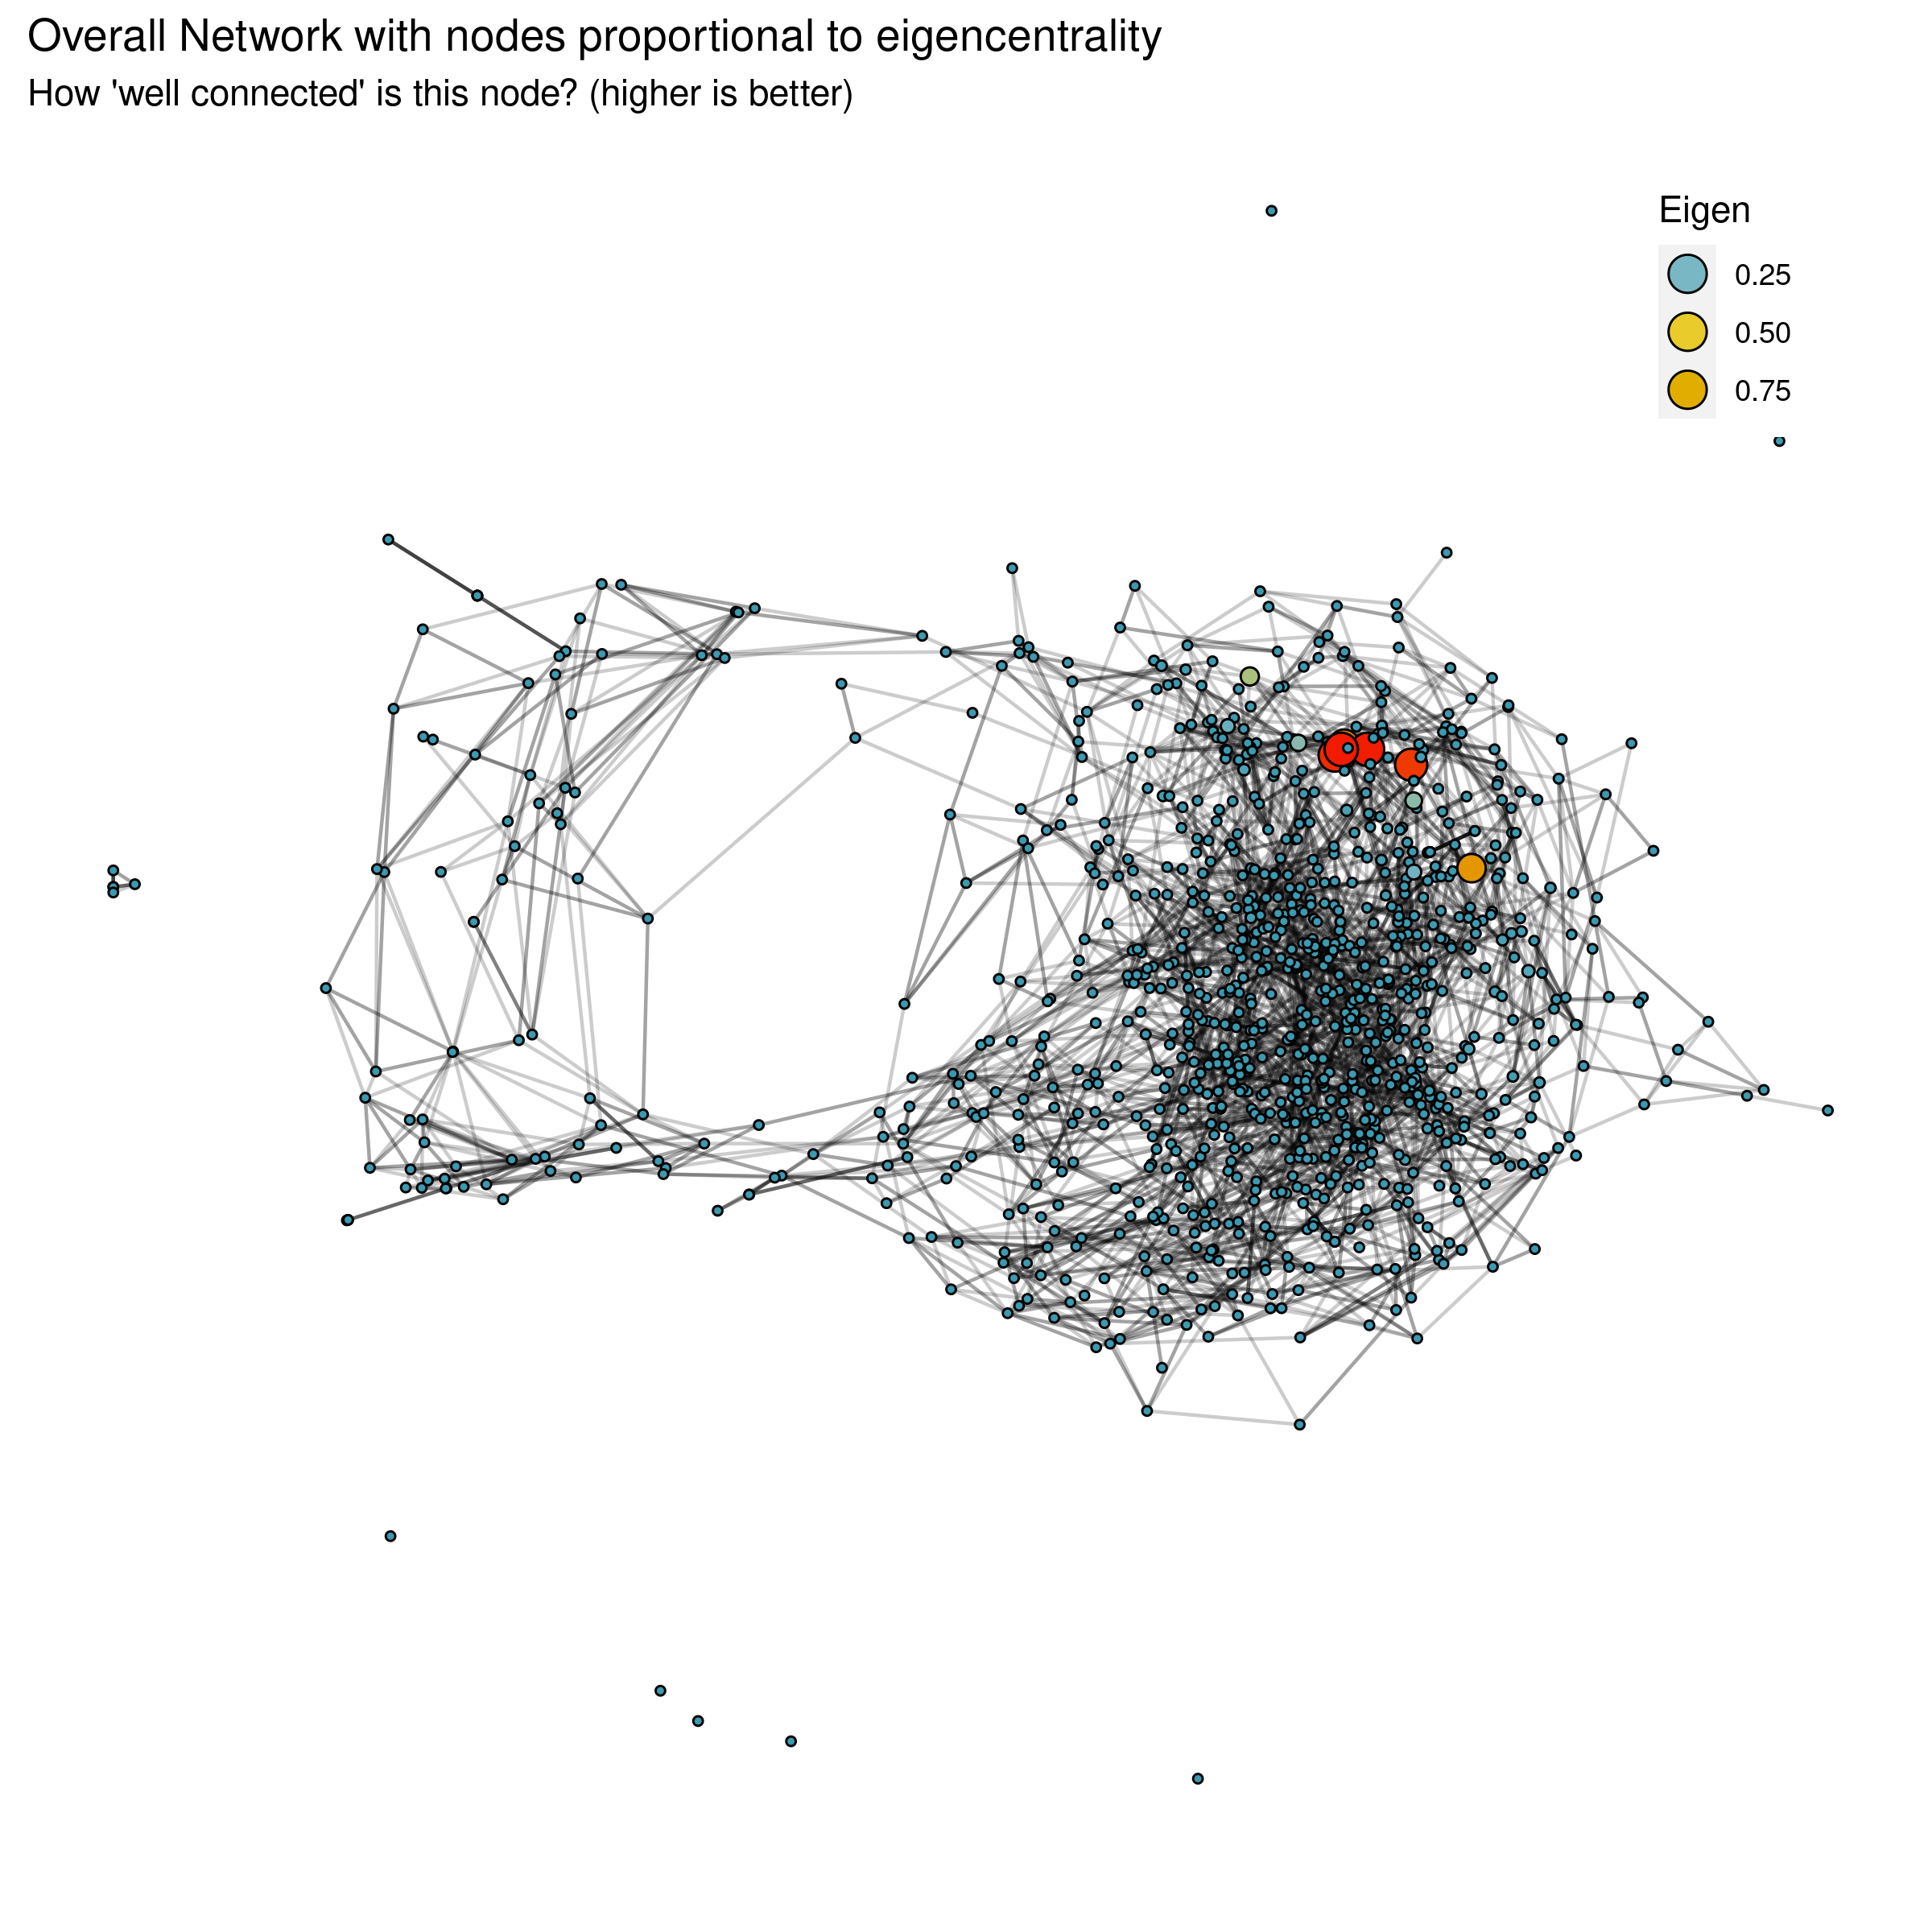
\includegraphics[width=0.9\linewidth]{figures/Networks/Centralities/Graph_overallEdgesDF_centralitiesDF_Eigen___mds.png} 
        \caption{Overall network coloring nodes by their eigencentrality. Node size is also proportional to eigencentrality. A few nodes are popular people also connecting to other popular people.}
        \label{figure:networksEigen}
    \end{figure}      

\subsubsection{Bonacich Centrality}
 
Is the same as Eigencentrality, but you get a decay factor the further away you are from well-connected people \cite{Bonacich1972}.

\subsection{Connectivity average}

Connectivity is the average chosen centrality per node in the network. It gives you an idea of how well the network is interconnected. Higher degree centrality numbers mean that information or diseases travel around much easier. In table \ref{table:networksHS} we can see that connectivity is not constant in the network, for example, some schools display higher connectivity than others, and the same goes for sex dynamics.

    \begin{figure}[h!]
        \centering
            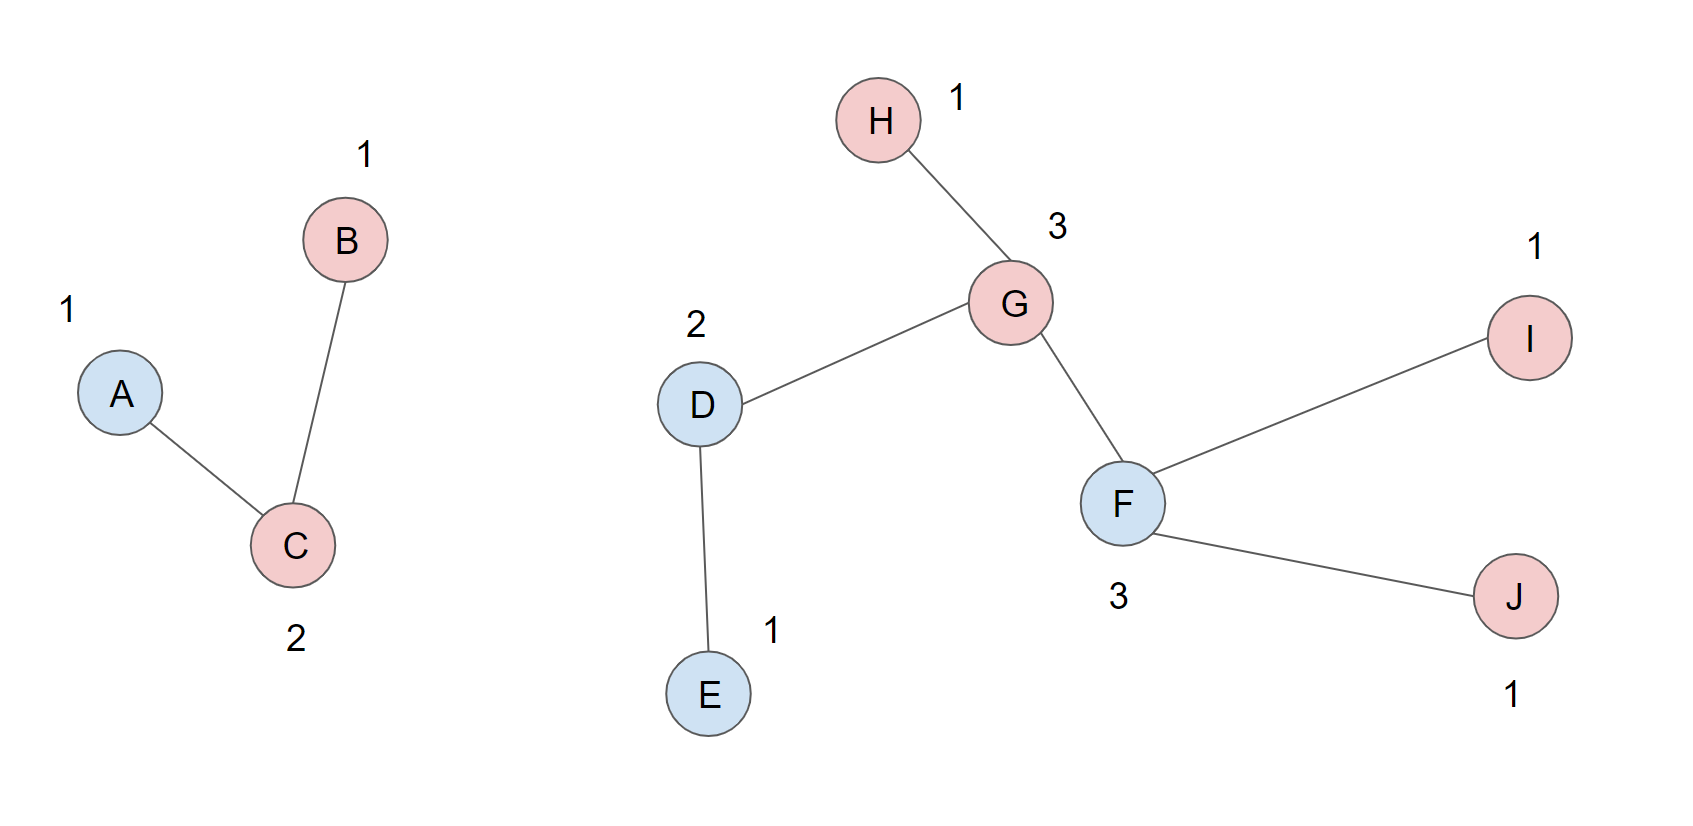
\includegraphics[width=0.7\linewidth]{figures/Networks/Concepts/edgesConnectivity.png} 
        \caption{A network with two components. Nodes are labeled with the number of degree centrality in each. On the left component, we have an average degree of 1.3, while in the right component, we have an average degree of 1.71}
        \label{figure:networksConnectivity}
    \end{figure}   

\label{figure:networksHS}
\begin{table}[h!]
    \centering
    \caption{The average centralities measures for the whole population, each high school, and also men and women. Notice that in H5 we have a higher amount of disconnected triads, which causes outliers in the average value for closeness.}
    \renewcommand{\arraystretch}{1.7}
    \begin{tabular}{rccccc|}
    \cline{2-6}
    \multicolumn{1}{l|}{}                                    & \multicolumn{1}{l}{\cellcolor[HTML]{FFFFC7}Degree} & \multicolumn{1}{l}{\cellcolor[HTML]{FFFFC7}Closeness} & \multicolumn{1}{l}{\cellcolor[HTML]{FFFFC7}Between} & \multicolumn{1}{l}{\cellcolor[HTML]{FFFFC7}Eigen} & \multicolumn{1}{l|}{\cellcolor[HTML]{FFFFC7}Bonacich} \\ \hline
    \multicolumn{1}{|l|}{\cellcolor[HTML]{FBDBB5}Population} & 5.34                                               & 0.0014                                                & 2362                                                & 0.0087                                            & -0.0215                                               \\ \hline
    \multicolumn{6}{|c|}{\cellcolor[HTML]{C0C0C0}High school}                                                                                                                                                                                                                                                                               \\ \hline
    \multicolumn{1}{|r|}{\cellcolor[HTML]{EFEFEF}H1}         & 5.4                                                & 0.0002                                                & 2696                                                & 0.0015                                            & -0.0155                                               \\
    \multicolumn{1}{|r|}{\cellcolor[HTML]{EFEFEF}H2}         & 5.06                                               & 0.0002                                                & 2197                                                & 0.0009                                            & 0.0084                                                \\
    \multicolumn{1}{|r|}{\cellcolor[HTML]{EFEFEF}H3}         & 5.51                                               & 0.0002                                                & 2501                                                & 0.0015                                            & -0.0423                                               \\
    \multicolumn{1}{|r|}{\cellcolor[HTML]{EFEFEF}H4}         & 5.44                                               & 0.0002                                                & 2033                                                & 0.0011                                            & -0.0154                                               \\
    \multicolumn{1}{|r|}{\cellcolor[HTML]{EFEFEF}H5}         & 4.95                                               & 0.0148                                                & 1913                                                & 0.0000                                            & 0.0689                                                \\
    \multicolumn{1}{|r|}{\cellcolor[HTML]{EFEFEF}H6}         & 4.23                                               & 0.0002                                                & 2258                                                & 0.0002                                            & -0.2174                                               \\
    \multicolumn{1}{|r|}{\cellcolor[HTML]{EFEFEF}H7}         & 5.76                                               & 0.0002                                                & 2526                                                & 0.0038                                            & 0.0294                                                \\
    \multicolumn{1}{|r|}{\cellcolor[HTML]{EFEFEF}H8}         & 5.1                                                & 0.0002                                                & 2132                                                & 0.0627                                            & -0.1456                                               \\ \hline
    \multicolumn{6}{|c|}{\cellcolor[HTML]{BCFBBB}Sex}                                                                                                                                                                                                                                                                                       \\ \hline
    \multicolumn{1}{|r|}{\cellcolor[HTML]{B7FDFA}Men}        & 5.31                                               & 0.0011                                                & 2405                                                & 0.0153                                            & -0.0106                                               \\
    \multicolumn{1}{|r|}{\cellcolor[HTML]{FFBED5}Women}      & 5.37                                               & 0.0017                                                & 2317                                                & 0.0019                                            & -0.0328                                               \\ \hline
    \end{tabular}
\end{table}


\subsection{Density}

Density is another overview of the number of relationships in a network. Is the amount of total connections divided by the amount of possible connections. Unlike connectivity, this value is bounded between 0 and 1. Density by itself is not an exciting metric and needs to be compared with another density to get some useful information. For example, we can compare the friendship density of the high schools in Northern Norway, with the density in Southern Norway to see if there is a significant difference. We can do the same for nodes inside a network, such as comparing the friendship density of men against the friendship density of women.

    \begin{figure}[h!]
        \centering
            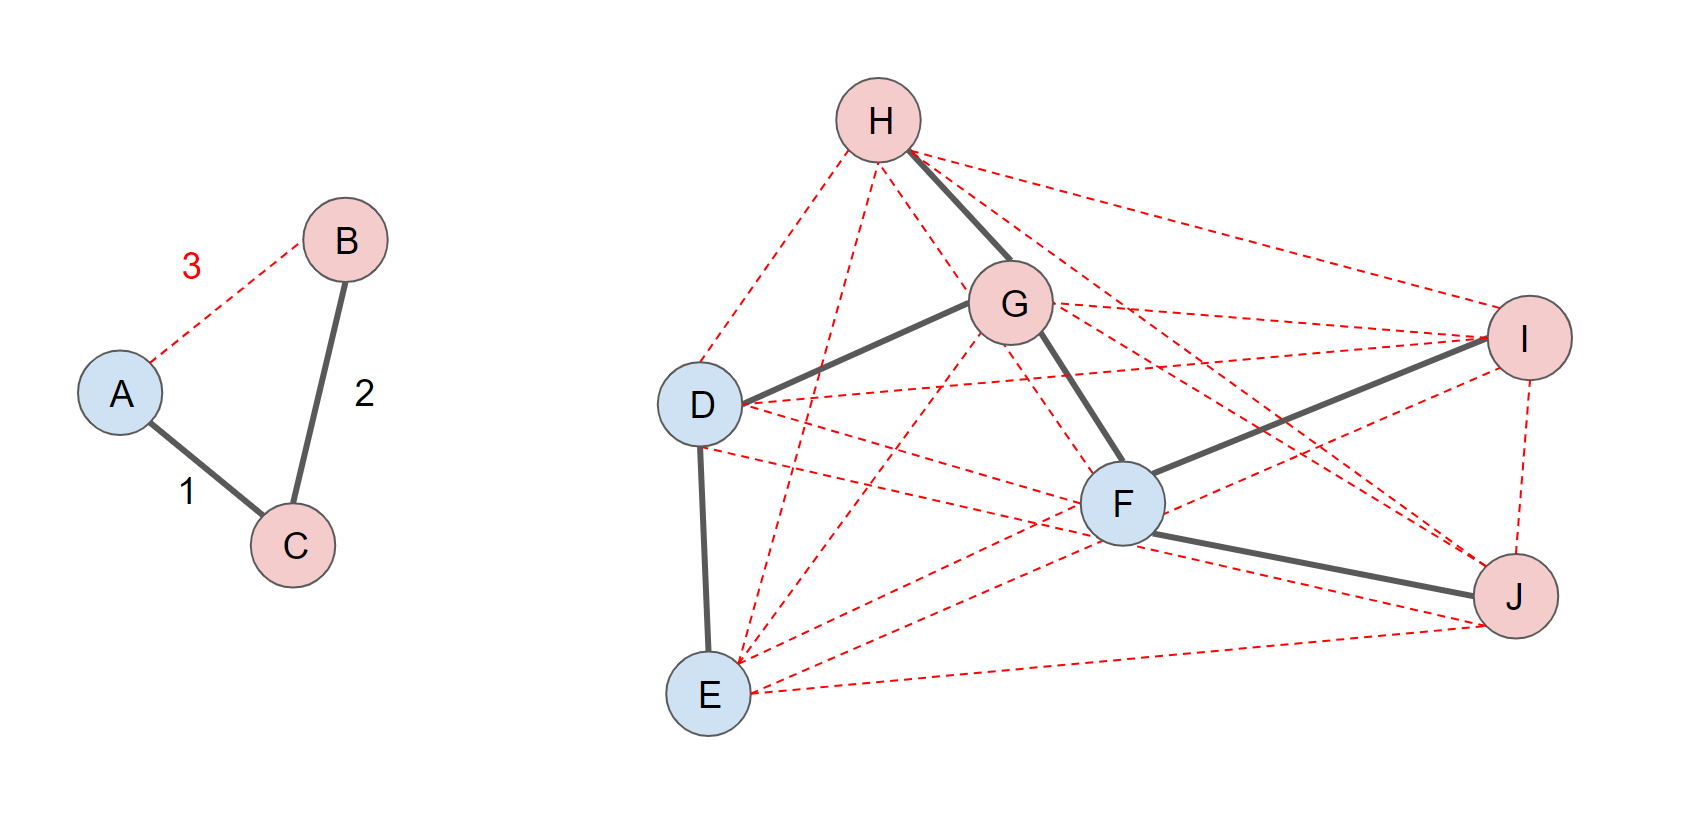
\includegraphics[width=0.7\linewidth]{figures/Networks/Concepts/edgesDensity.png} 
        \caption{A network with two components. Black edges thick represent existing edges, and red thin and dashed edges represent possible edges. On the left component, the 3 possible edges are shown and labeled. On the right component, no edge is labeled. The left component has a density of 2/3 (66\%), while the right component has a density of 6/49 (12\%). Notice that the right component, despise having higher average connectivity, also has a lower density.}
        \label{figure:networksDensity}
    \end{figure}    


\subsection{Homophily}
\label{network:homophily}

Homophily is the core reason why social network studies work. Individuals tend to form strong bonds with people who are similar to them by factors such as marital status, race, economics, nationality, common interests, and many more \cite{Stehl2013, Moody2001, Qian2007, Cheadle2012, McPherson1987, Sergio2009, Kossinets2009, McPherson2001, Smith2014, Karimi2018, Lee2019, Avin2020, Asikainen2020}. This is also the biggest challenge when interpreting data, as we cannot be sure if individuals who are close to each other are influencing each other, or if they are simply sharing an environmental factor that influences everyone at the same time to no fault of the nature of their relationships.

Homophily is the ratio of, nodes that have an edge to another node that has the same property, against nodes that have an edge to a node of different property. Density only cares that there's an edge, while homophily cares about what types of nodes are being connected. Similar to density, homophily needs to be compared to another homophily number to gain some useful information.

First, we define edges that connect two nodes with the same attributes:
    \begin{equation}
        H_{any} \subseteq  \left\{ (x,y) | (x,y) \in V^2  \land x \neq y  \land x_i = y_i \right\}
    \end{equation}
Second, we define edges that connect two nodes with the same given attribute:
    \begin{equation}
        H_{given} \subseteq  \left\{ (x,y) | (x,y) \in V^2  \land x \neq y  \land x_i = y_i = A \right\}      
    \end{equation}
Finally, we define edges that connect two nodes with either of them having a GIVEN attribute:
    \begin{equation}
        H_{either} \subseteq  \left\{ (x,y) | (x,y) \in V^2   \land  x \neq y \land  x_i = A | y_i = A \right\}
    \end{equation}    
For a given variable, there are two ways to calculate homophily:
    \begin{equation}
        Homophily_i =  \frac{|H_{any}|}{|E|}
    \end{equation}
    \begin{equation}
        Homophily_{i=A} =  \frac{|H_{given}|}{|H_{either}|}      
    \end{equation}
In figure \ref{figure:networkExampleWeights}, we have 9 edges. Edges \{B,C\} and \{H,G\} connect red to red. Edges \{A,D\} and \{D,E\} connect blue to blue. Therefore, we have 4 edges connecting the same colors out of 9 possible. $Homophily_{color} = 44.4\%$ . Specifically for red, we have the same edges \{B,C\} and \{H,G\} connecting red to red, and edges \{A,C\}, \{B,C\}, \{D,G\}, \{H,G\}, \{G,F\}, \{F,I\} and \{F,J\} connecting at least one red. Then, $Homophily_{color = red} = 28.6\%$.

Is also possible to do a binomial test on the homophily to check if it is significant. This is simply measuring how many nodes of the same attributes we have, and how many are friends between them. If the number of edges is proportional to the number of nodes, that indicates that the number of relationships within the same group is what we would expect by random chance. But if we have too little, or too many relationships among them, it might indicate that the group is biased toward forming relationships among themselves or avoiding each other. Following the figure \ref{figure:networkExampleWeights} example:

    \begin{itemize}
        \item How many edges are reds friending red? 2
        \item How many reds do we have? 6
        \item What is the probability of being red? 0.6 
    \end{itemize}

The calculated binomial test is:
    \begin{equation*}
         \dbinom{6}{2} \cdot 0.6^2 \cdot (1-0.6)^{6-2} = 0.14
    \end{equation*}
The probability $Homophily_{color = red} = 0.286$ is greater than we would expect by chance (0.14), however, is not greater by much. The p-value for a two-sided test is 0.23 indicating that we can't really tell if the reds are biased in this graph.

\subsection{Average path length}

For fully connected networks, the \gls{apl} is the average of all possible paths. If a network is not fully connected, then the average path length is infinite. In such cases is more interesting to find the APL per sub-network. \gls{apl} is related to density. Forming 4 different interesting cases:

\begin{itemize}
    \item  Low \gls{apl} and low density will have a close solution to a minimum spanning tree. This is a subset of edges that connects all the nodes without cycles and with the minimum possible edges or edge weight. This case is important because it shows the cheapest way to lay down roads connecting cities so all cities are connected, expending the least amount of money possible.
    \item  High \gls{apl} and low density mean all the nodes are connecting using very few edges. This is bad if we describe for example a network of roads, because it will have very long paths and at the same time all cars need to pass through the same common edges. This is good if we have an infectious disease because it means we can cut the network in half easily and avoid propagation.
    \item  Low \gls{apl} and high density. This case means that all the nodes are very well connected, and traveling from one to another is easy. As opposed to before, great for roads due to low traffic, but bad for diseases because is very difficult to slow down or stop the spread.
    \item  High \gls{apl} and high density. This means that you have many sub-networks that are very well connected, but the connection between sub-networks is done with a really low number of edges forming choking points.
\end{itemize}

\subsection{Coverage}

Coverage of a node refers to how many nodes you can reach from that particular node in equal or less a particular path distance. This is also referred to as how many steps you need to reach any given pair of nodes if their distances are all equal.

    \begin{figure}[h!]
        \centering
            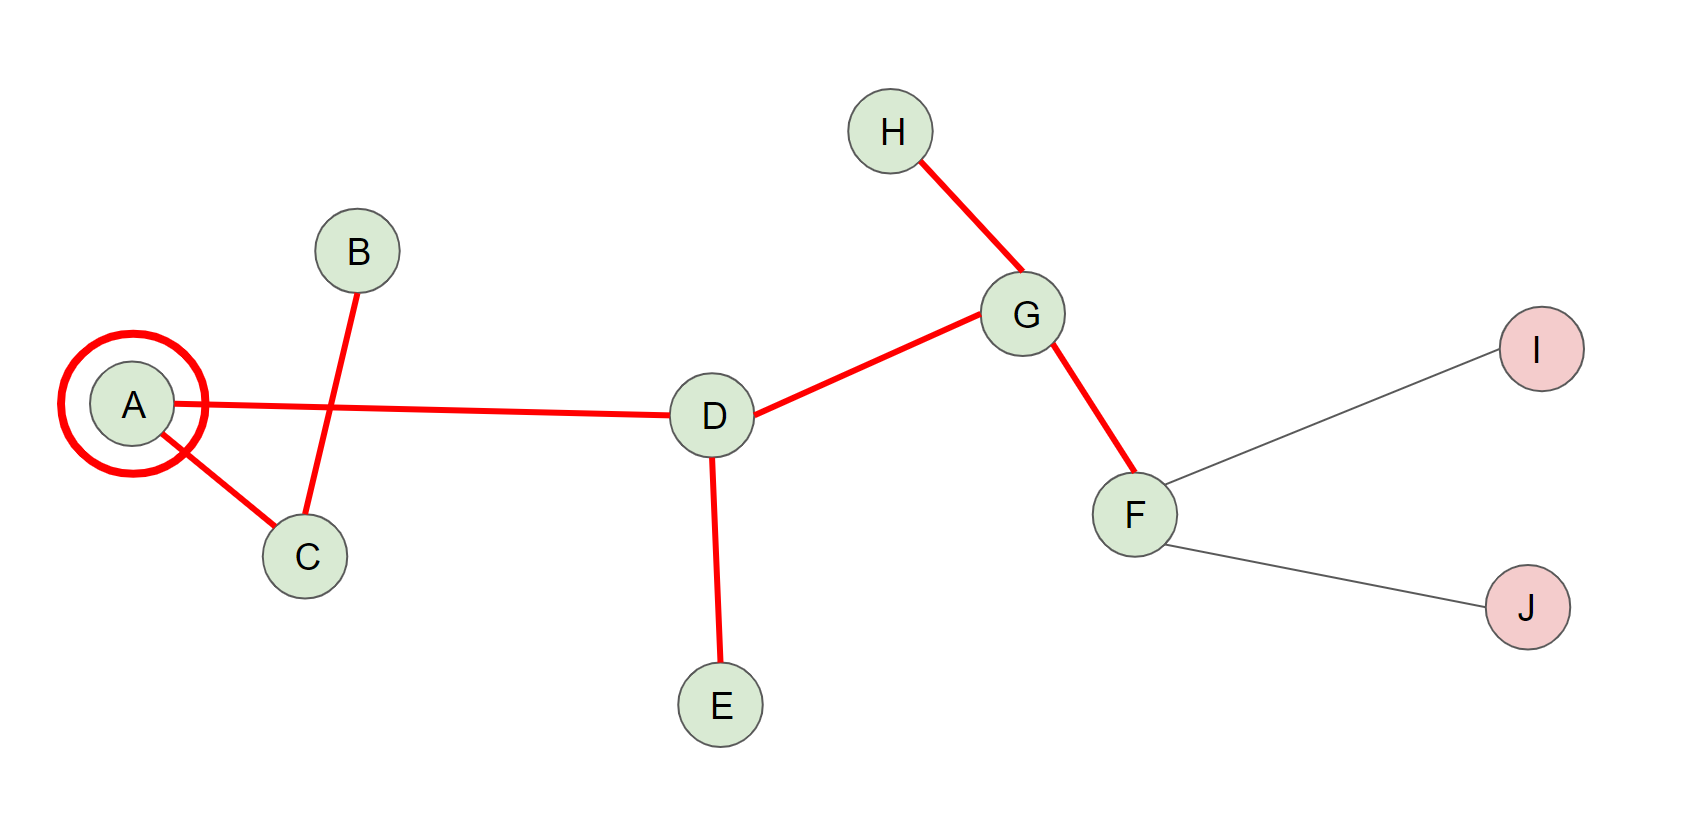
\includegraphics[width=0.7\linewidth]{figures/Networks/Concepts/coverage.png} 
        \caption{An example of coverage. For a given path of distance equal to 3, node A can reach all the green highlighted nodes using the red highlighted paths.}
        \label{figure:networkCoverage}
    \end{figure}

\subsection{Reachability}

Reachability refers to the average coverage per step in a network. Reachability is related to connectivity, as the network is more and more dense, is more easy to cover more nodes with fewer steps. This is an important variable when we deal with infectious diseases, if a large area of the network is reachable very quickly, the disease will spread very quickly as well.

    \begin{figure}[h!]
        \centering
            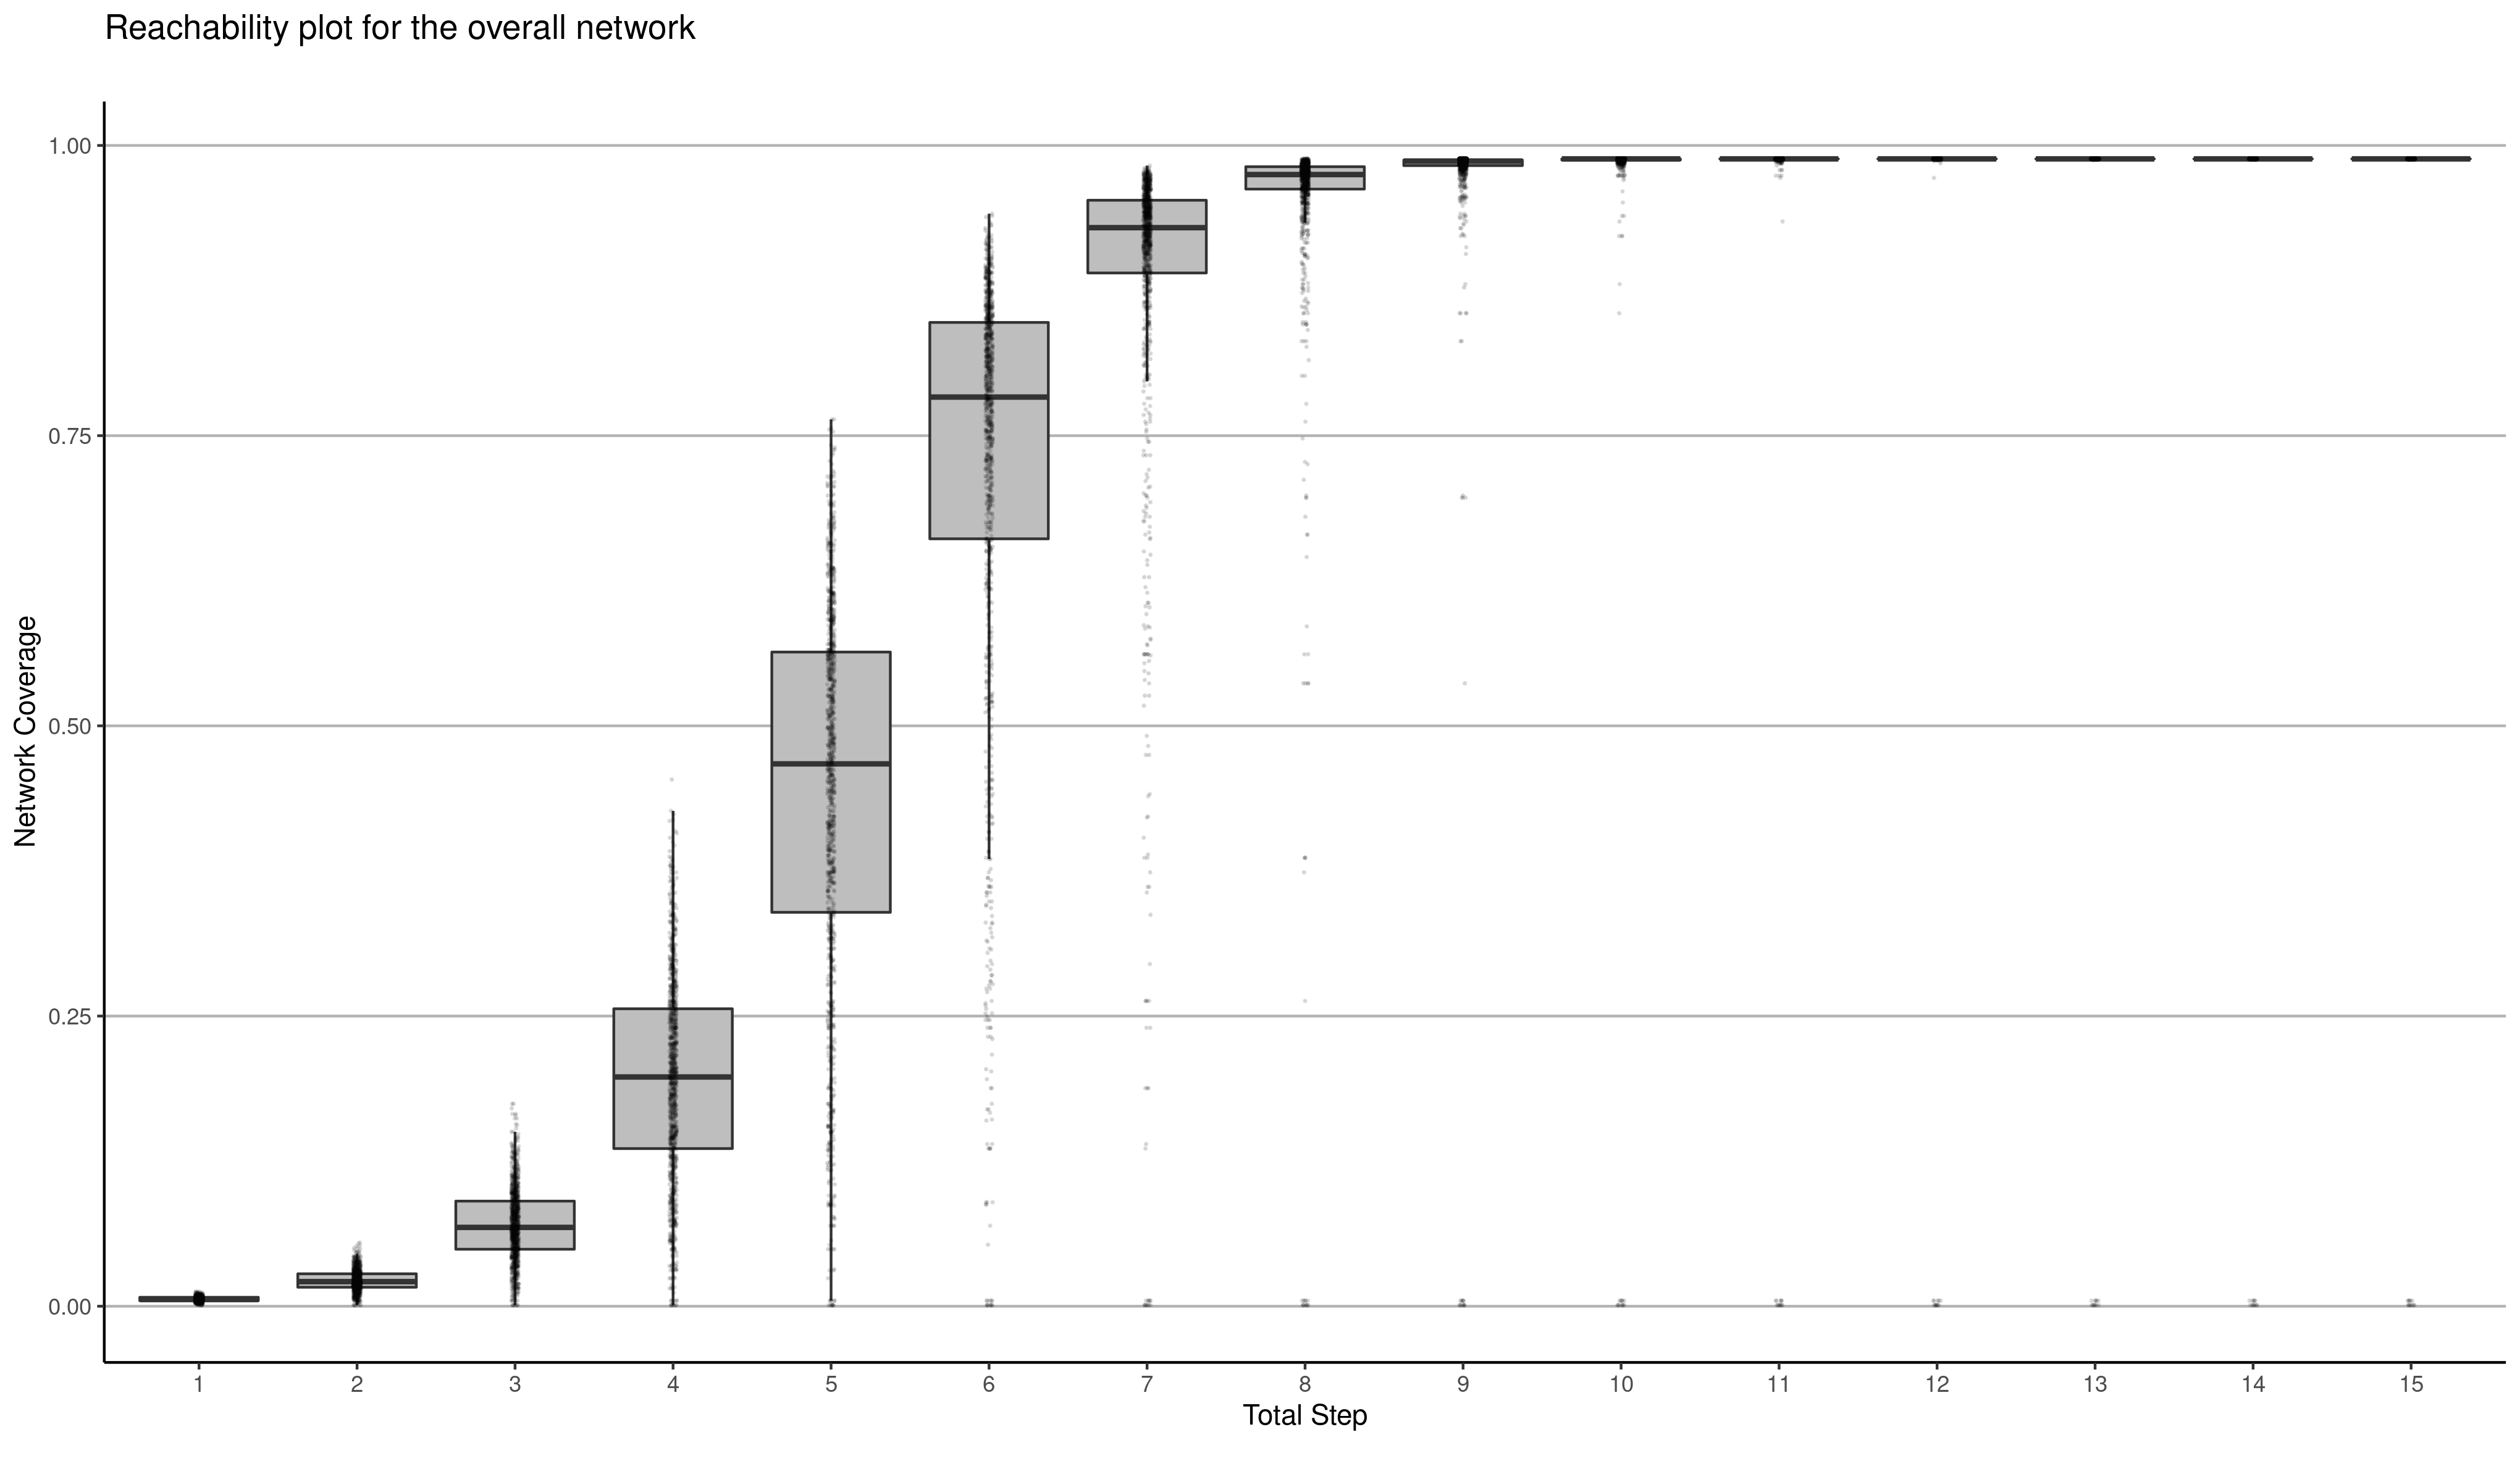
\includegraphics[width=0.7\linewidth]{figures/Networks/Reach/CategoricalBoxplot_reachplot_variable_value.png} 
        \caption{A reachability plot in the overall network. The x-axis represents the number of steps taken. The y-axis represents the proportion of network coverage. After 4 steps, we see that about 25\% of the nodes manage to cover 25\% of the network. In the next step, nearly 50\% of the nodes, cover 50\% of the network. In the next step, we see that the median surpasses the 75\% coverage, so the nodes reach grows exponentially in this network. It never reaches 100\% because some of the nodes are isolated, we see this better in the outliers that start showing from step 7 at the bottom of each box.}
        \label{figure:networksReach}
    \end{figure}    

\subsection{Simulations}

Finally, let's talk about how all these concepts can be put together in a practical case, which is how a disease can advance through the network. This topic has already been studied, to the point that even a zombie apocalypse has been described and published. \cite{Munz2009WHENZA}

%When zombies attack!:  Mathematical modelling of an outbreak of zombie infection Philip Munz, Ioan Hudea, Joe Imad, Robert J. Smith

We can apply the same method to our network, to which we made a simulation engine capable of performing with the following infectious parameters:

\begin{itemize}

    \item What is the probability of any given person being able to spread the disease to another connected person? (ie: do they stay in contact often? is the person using face masks?)
    
    \item What is the probability of a person receiving the disease? (ie: Does he wash his hands often? is he immunocompromised?)
    
    \item What is the probability of passing the disease and immunizing yourself once you are infected? How does this change over time? (ie: the Polio vaccine gives lifelong immunity, whereas chickenpox last for about 10 to 15 years)
    
    \item What is the probability of dying for each person? Does this increase over time once infected? (ie: comorbidity factors such as obesity and COVID-19)
    
    \item Is this disease recurrent? (ie: Epstein–Barr virus)
    
    \item Is this due to a biphasic virus? (ie: tick-borne encephalitis)
    
    \item Do we allow random jumps in the network? (ie: airborne diseases)
    
    \item How long until we develop a vaccine? How many can be vaccinated each unit of time?
    
\end{itemize}

For this example, we generated an unknown novel disease that has a 30\% chance of transmission from person to person, as long as they are connected in the overall network. People can get immunized at any time and have a 10\% chance of doing so, but they can also die at any time and have a 1\% of so. We study six cases with 200 simulations each, one in which the disease follows its natural order, and the other five applying a vaccine to the population at step 10, with the restriction that we only have 30 vaccines per step.  The vaccine is administered to people that we know that have never shown signs of infection, don't currently have the disease, didn't have the disease in the past, and are not dead. The vaccine is 100\% effective and has no side effects. In the first vaccine case, we give the vaccine at random, the second case we give the vaccine first to people with a higher degree of centrality (most friends), third case higher closeness (shorter distance to rest of nodes), fourth case higher betweenness (connecting subnetworks), and fifth case higher eigencentrality (important people). The results for this simulation can be found in table \ref{table:networkSimulations} 

\begin{table}[H]
    \centering
    \label{table:networkSimulations}
    \caption{Comparison between the different simulation results. The first two cases can be seen in figure \ref{figure:simulationsA} , and figure \ref{figure:simulationsB}. Death rate and immunity rate is calculated at the final step of the simulation. Peak infection is calculated with respect the maximum infection coverage in each simulation, and in which step did happen.}
    \renewcommand{\arraystretch}{1.7}
    \scalebox{0.7}{
    \begin{tabular}{rc|ccccc|}
    \cline{3-7}
                                                                      & \multicolumn{1}{l|}{}              & \multicolumn{5}{c|}{\cellcolor[HTML]{FFFC9E}Vaccines at step = 10 , 30 / step}                                                                                             \\ \cline{2-7} 
    \multicolumn{1}{r|}{}                                             & \cellcolor[HTML]{EFEFEF}No vaccine & \cellcolor[HTML]{FFFFC7}Random & \cellcolor[HTML]{FFFFC7}Degree & \cellcolor[HTML]{FFFFC7}Closseness & \cellcolor[HTML]{FFFFC7}Betweenness & \cellcolor[HTML]{FFFFC7}Eigen \\ \hline
    \rowcolor[HTML]{FFFFFF} 
    \multicolumn{1}{|r|}{\cellcolor[HTML]{C0C0C0}Total death (n)}     & 66 ± 38                              & 23 ± 19                          & 18 ± 15                          & 18 ± 17                              & 16 ± 15                               & 26 ± 19                         \\
    \rowcolor[HTML]{FFFFFF} 
    \multicolumn{1}{|r|}{\cellcolor[HTML]{C0C0C0}Death rate (\%)}     & 6.30 ± 3.57                        & 2.17 ± 1.77                    & 1.71 ± 1.39                    & 1.70 ± 1.55                          & 1.53 ±  1.39                          & 2.49 ± 1.80                     \\
    \rowcolor[HTML]{FFFFFF} 
    \multicolumn{1}{|r|}{\cellcolor[HTML]{96FFFB}Immunity rate (\%)}  & 62.15 ± 34.51                      & 97.85 ± 1.73                    & 98.35 ± 1.33                   & 98.31 ± 1.51                         & 98.51 ± 1.34                          & 97.54 ± 1.74                    \\
    \rowcolor[HTML]{FFFFFF} 
    \multicolumn{1}{|r|}{\cellcolor[HTML]{FFCCC9}Peak infection (\%)} & 32.71 ± 18.29                      & 12.23 ± 9.99                   & 10.08 ± 8.16                   & 9.10 ± 8.52                          & 9.21 ± 8.33                           & 13.98 ± 10.29                   \\
    \rowcolor[HTML]{FFFFFF} 
    \multicolumn{1}{|r|}{\cellcolor[HTML]{FFCCC9}at step}             & 23.20 ± 10.65                      & 19.15 ± 7.67                   & 17.47 ± 6.00                   & 17.21 ± 8.70                         & 15.86 ± 6.97                          & 19.35 ± 9.05                    \\ \hline
    \end{tabular}
    }
\end{table}

In the first case (figure \ref{figure:simulationsA}) if we are lucky, the disease will start in an isolated node, however, the overall immunity will be very low with the subsequence risk of the disease restarting again in a more connected node. We can also see that both the peak infection and death rates are quite high, with about 66 students dying on average.

    \begin{figure}[h!]
        \centering
            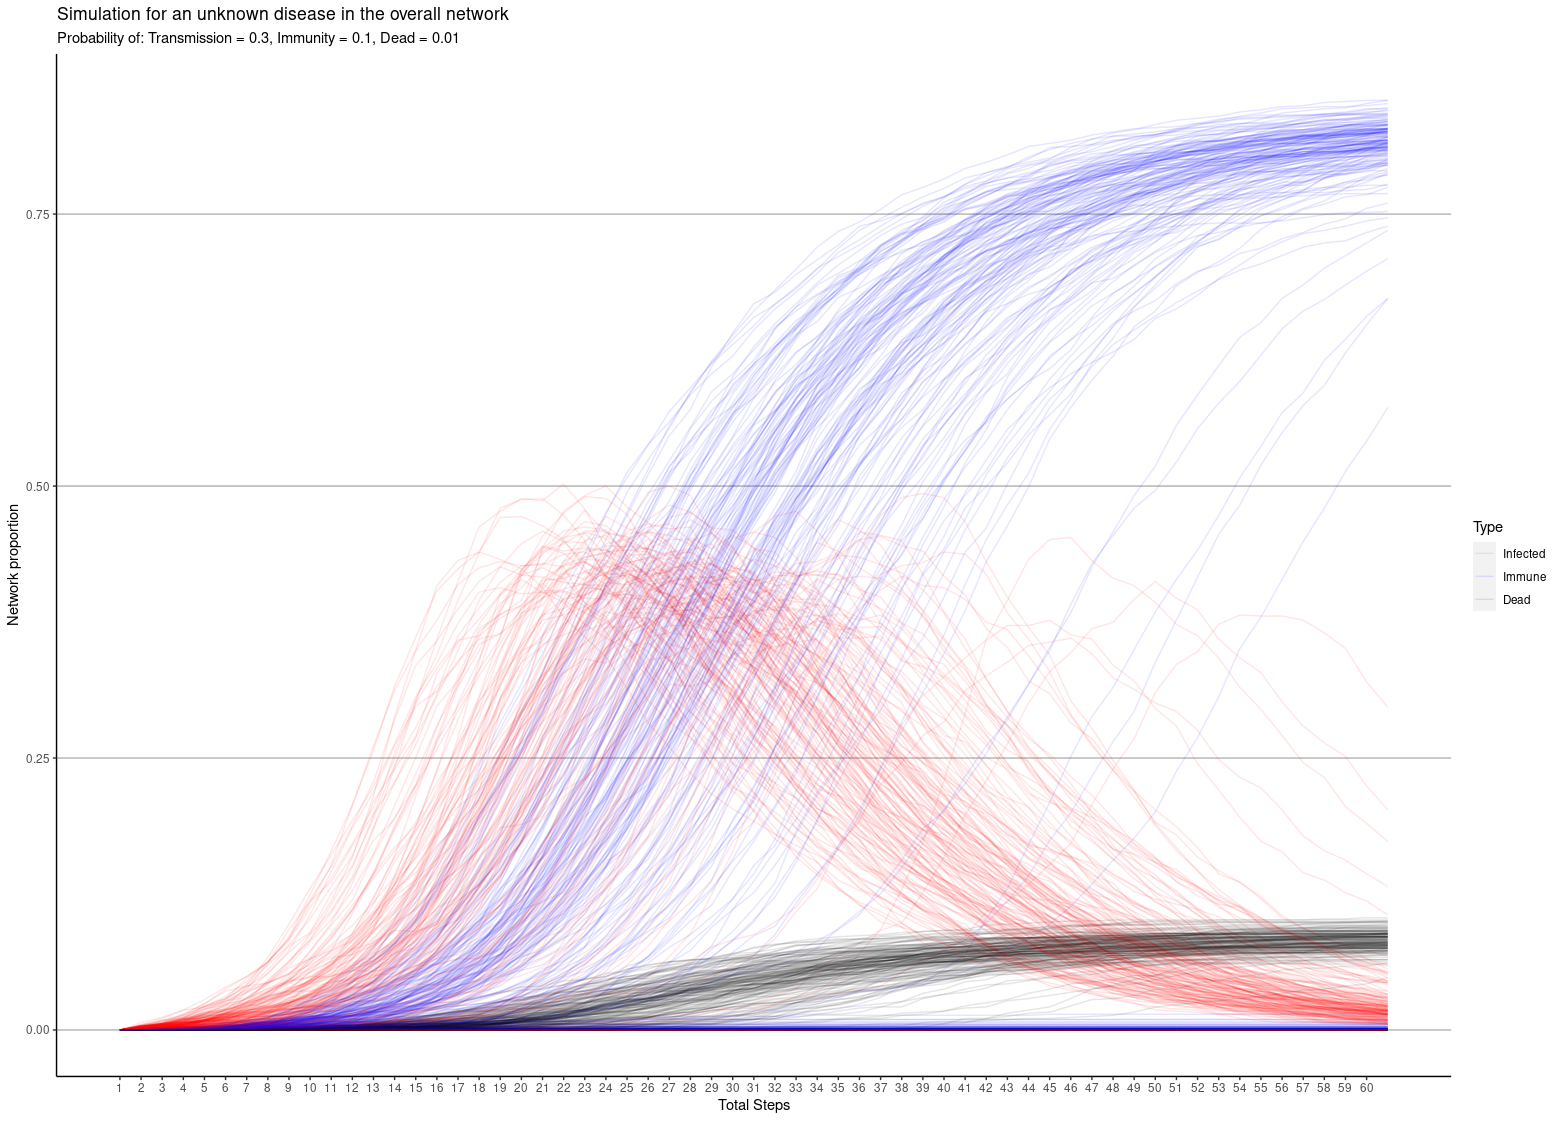
\includegraphics[width=0.95\linewidth]{figures/Networks/Simulations/Simulation_Nothing.png} 
        \caption{Simulation of the spread of an unknown disease in the network. In the x-axis, we have steps which is an arbitrary representation of time. In the y-axis the proportion of the network that each category has at any given time. Each red, blue, and red, line represent one of the 200 simulations. Red represents infected, Blue represents immunized, and Black represents dead.}
        \label{figure:simulationsA}
    \end{figure}   


For the second case (figure \ref{figure:simulationsB}), we introduce a vaccine. As expected the death rate drops dramatically, with about 23 students dying on average and an almost entirely immunized population in all cases. The peak of infections is reduced by more than half and is easier to predict when the worse time is going to happen.

    \begin{figure}[h!]
        \centering
            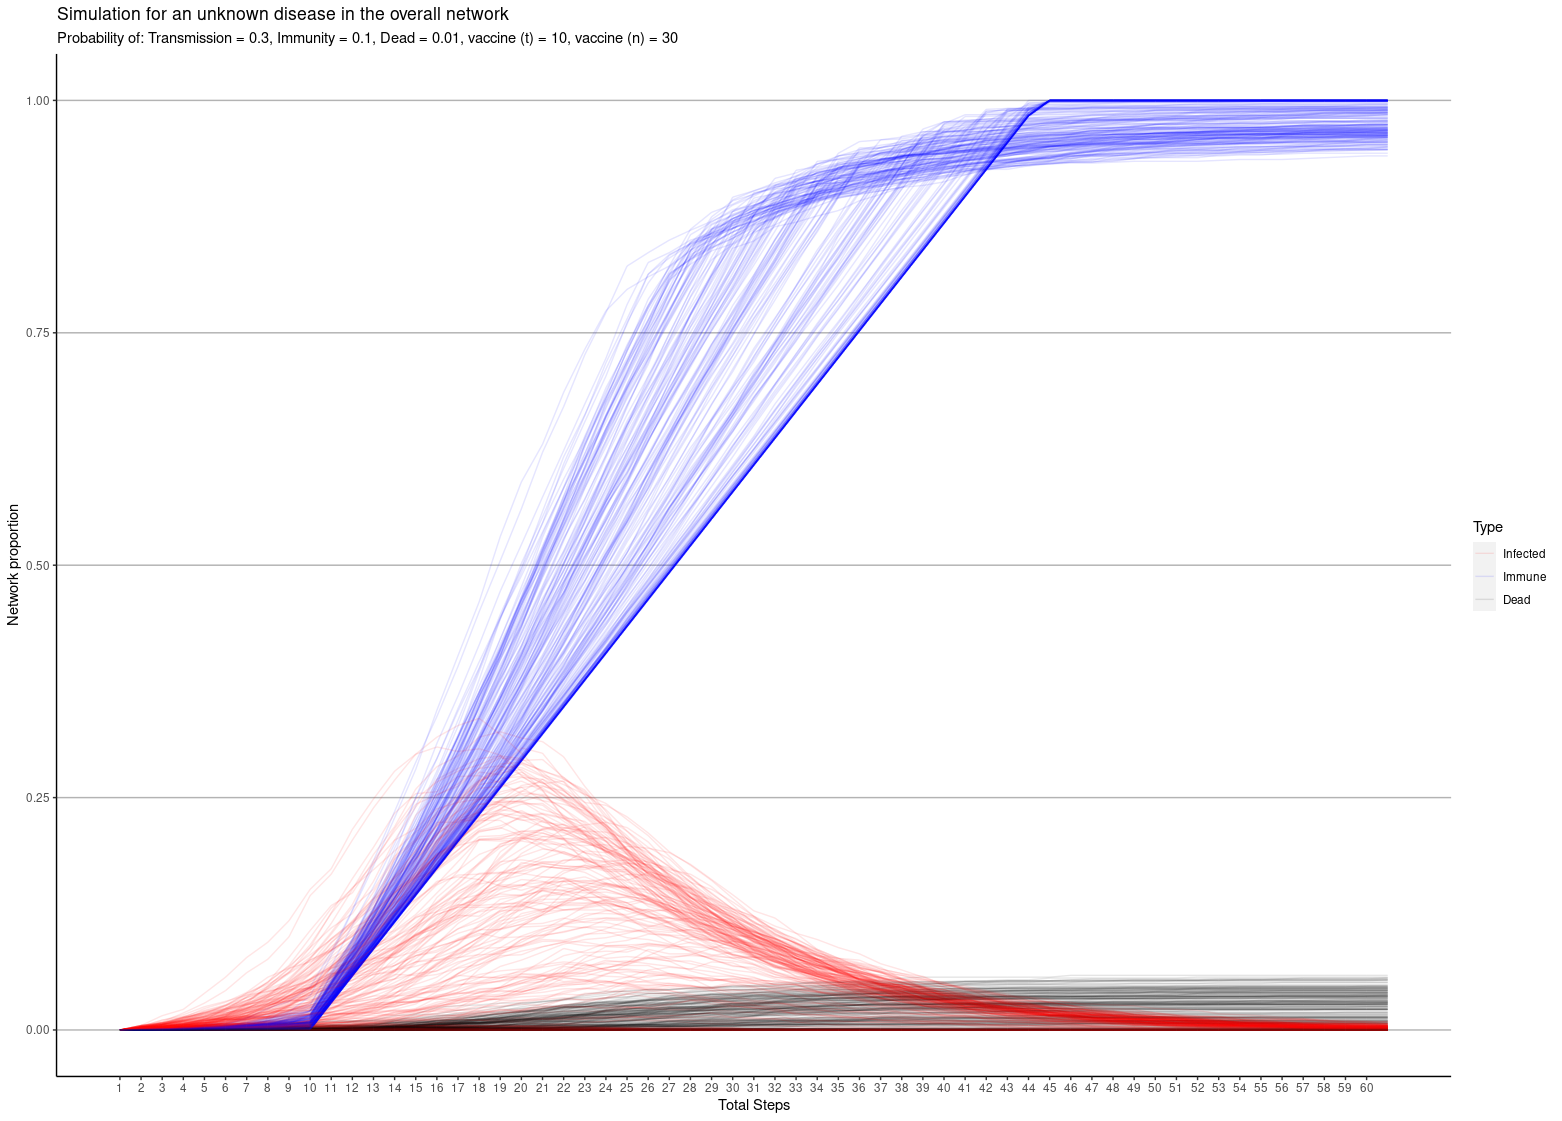
\includegraphics[width=0.95\linewidth]{figures/Networks/Simulations/Simulation_Vaccine_30.png} 
        \caption{Simulation of the spread of an unknown disease in the network. In the x-axis, we have the steps in time. In the y-axis the proportion of the network that each category has at any given time. Each red, blue, and red, line represent one of the 200 simulations. Red represents infected, Blue represents immunized, and Black represents dead. A vaccine is introduced at t = 10 which suddenly spikes the immunization ratio and lower dead rate}
        \label{figure:simulationsB}
    \end{figure}  

The rest of the cases produce similar figures with the slope of immunity being a bit more or less pronounced. The best results are when we apply the vaccine to people connecting subnetworks, in that way, we can isolate the disease very quickly. Notice that the number of deaths is lower when we immunize first people connecting sub-networks together (n = 16), rather than just giving it first to the most well-connected people (n = 18), which suggests that having prior knowledge of the network topology can help to safe lives.

    %\begin{figure}[h!]
     %   \centering
      %      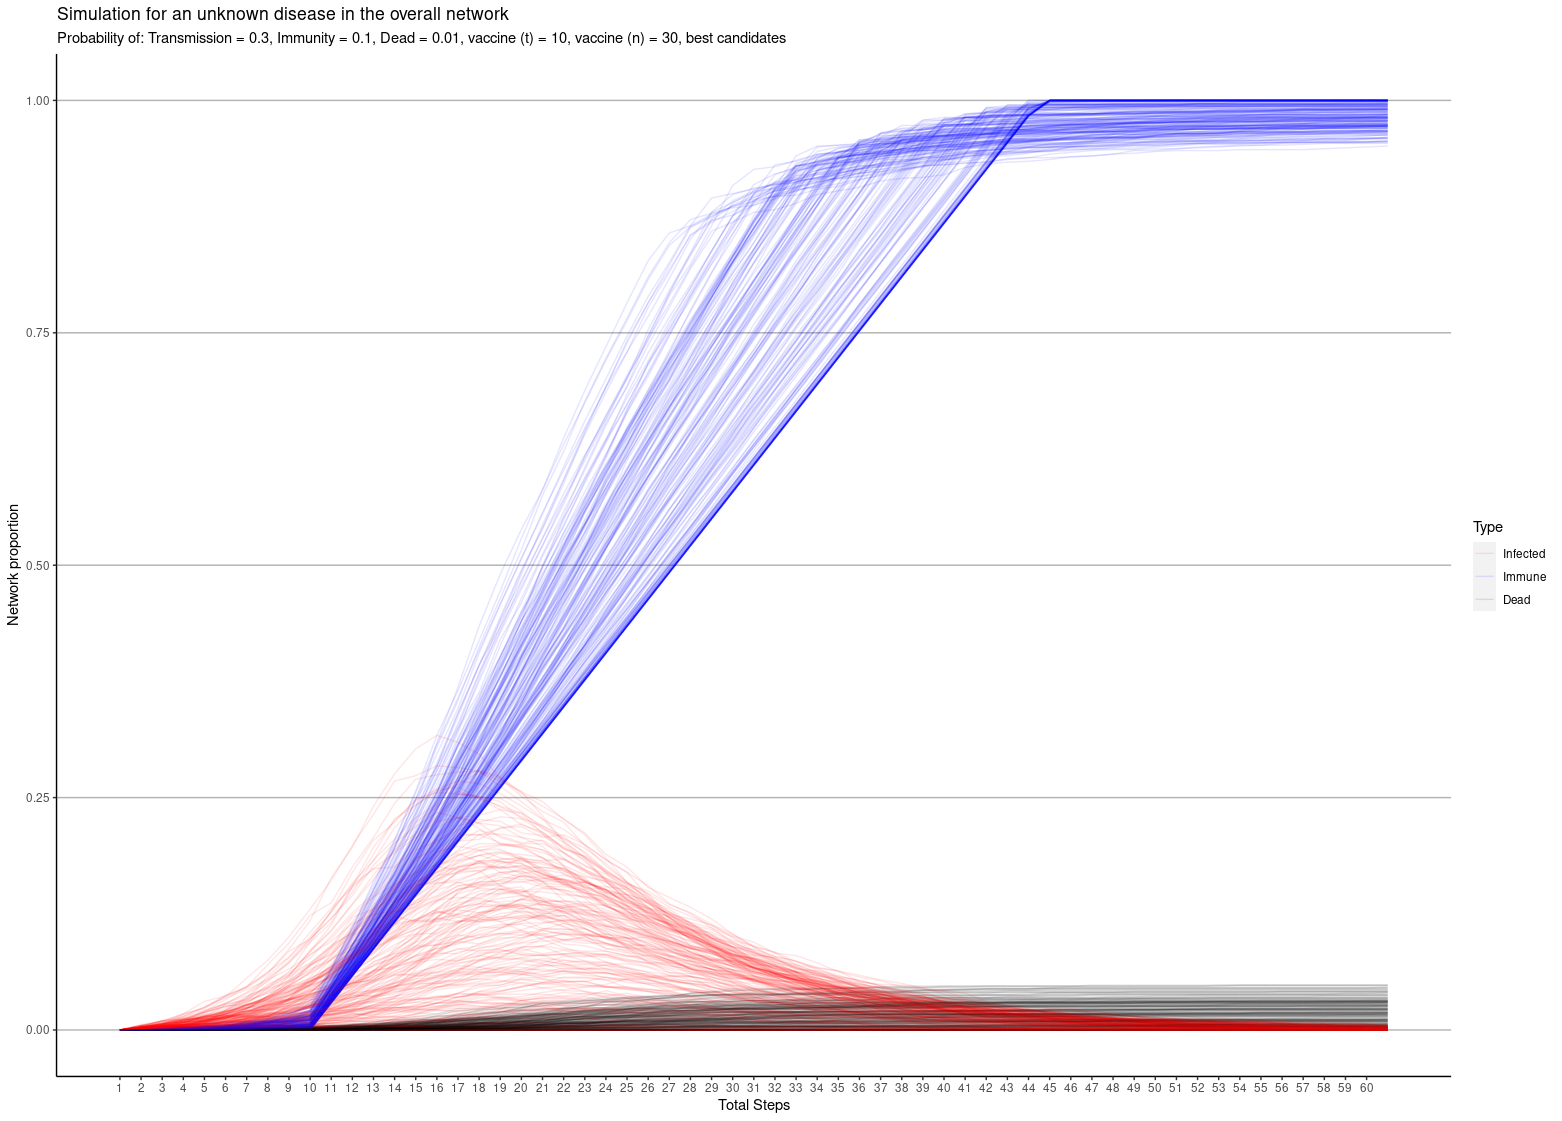
\includegraphics[width=0.95\linewidth]{figures/Networks/Simulations/Simulation_Best_30.png} 
       % \caption{Simulation of the spread of an unknown disease in the network. In the x-axis, we have the steps in time. In the y-axis the proportion of the network that each category has at any given time. Each red, blue, and red, line represent one of the 200 simulations. Red represents infected, Blue represents immunized, and Black represents dead. A vaccine is introduced at t = 10, but is given to the highest connected students first}
        %\label{figure:simulationsC}
    %\end{figure}  





%Nothing

%[1] "-------------"
%[1] "Mean Immunity:       0.621459537572254 +- 0.345102052201196"
%[1] "Mean Dead:           0.0629624277456647 +- 0.0357281205280136"
%[1] "Mean max infections: 0.327105009633911 +- 0.182383294477629"
%[1] "at time:             23.2 +- 10.6568212519484"

% Vaccine 30
%[1] "-------------"
%[1] "Mean Immunity:       0.978468208092486 +- 0.017343662559995"
%[1] "Mean Dead:           0.0216955684007707 +- 0.0177364552599782"
%[1] "Mean max infections: 0.122263969171484 +- 0.0998856407568371"
%[1] "at time:             19.145 +- 7.66929366543185"


% Best 30
%1] "-------------"
%[1] "Mean Immunity:       0.983482658959538 +- 0.0133188475582221"
%[1] "Mean Dead:           0.0170857418111753 +- 0.013902438604357"
%[1] "Mean max infections: 0.100770712909441 +- 0.0815998034228179"
%[1] "at time:             17.47 +- 6.00662113733147"

% Best Betweeness 30
%[1] "-------------"
%[1] "Mean Immunity:       0.985134874759152 +- 0.0134353361062699"
%[1] "Mean Dead:           0.0153131021194605 +- 0.0139325719338487"
%[1] "Mean max infections: 0.0920905587668593 +- 0.0832644828832967"
%[1] "at time:             15.855 +- 6.96754680951004"

% Best Closeness 30
% [1] "-------------"
% [1] "Mean Immunity:       0.983111753371869 +- 0.0150894772699903"
% [1] "Mean Dead:           0.0169701348747592 +- 0.0154606868655294"
% [1] "Mean max infections: 0.0909826589595376 +- 0.0851839777319293"
% [1] "at time:             17.205 +- 8.70354718883868"

% Best Eigen 30
% [1] "-------------"
% [1] "Mean Immunity:       0.975375722543353 +- 0.0174053731268066"
% [1] "Mean Dead:           0.0248603082851638 +- 0.017978236810753"
% [1] "Mean max infections: 0.139797687861272 +- 0.102859340836389"
% [1] "at time:             19.345 +- 9.04516723180154"
    
We also have the option of running this type of analysis against any layout of any network and making a comprehensive video simulation. This can be seen in figure \ref{fig:networkVideo}.

\begin{figure}[ht]
    \centering
    \begin{minipage}[b]{0.45\linewidth}
        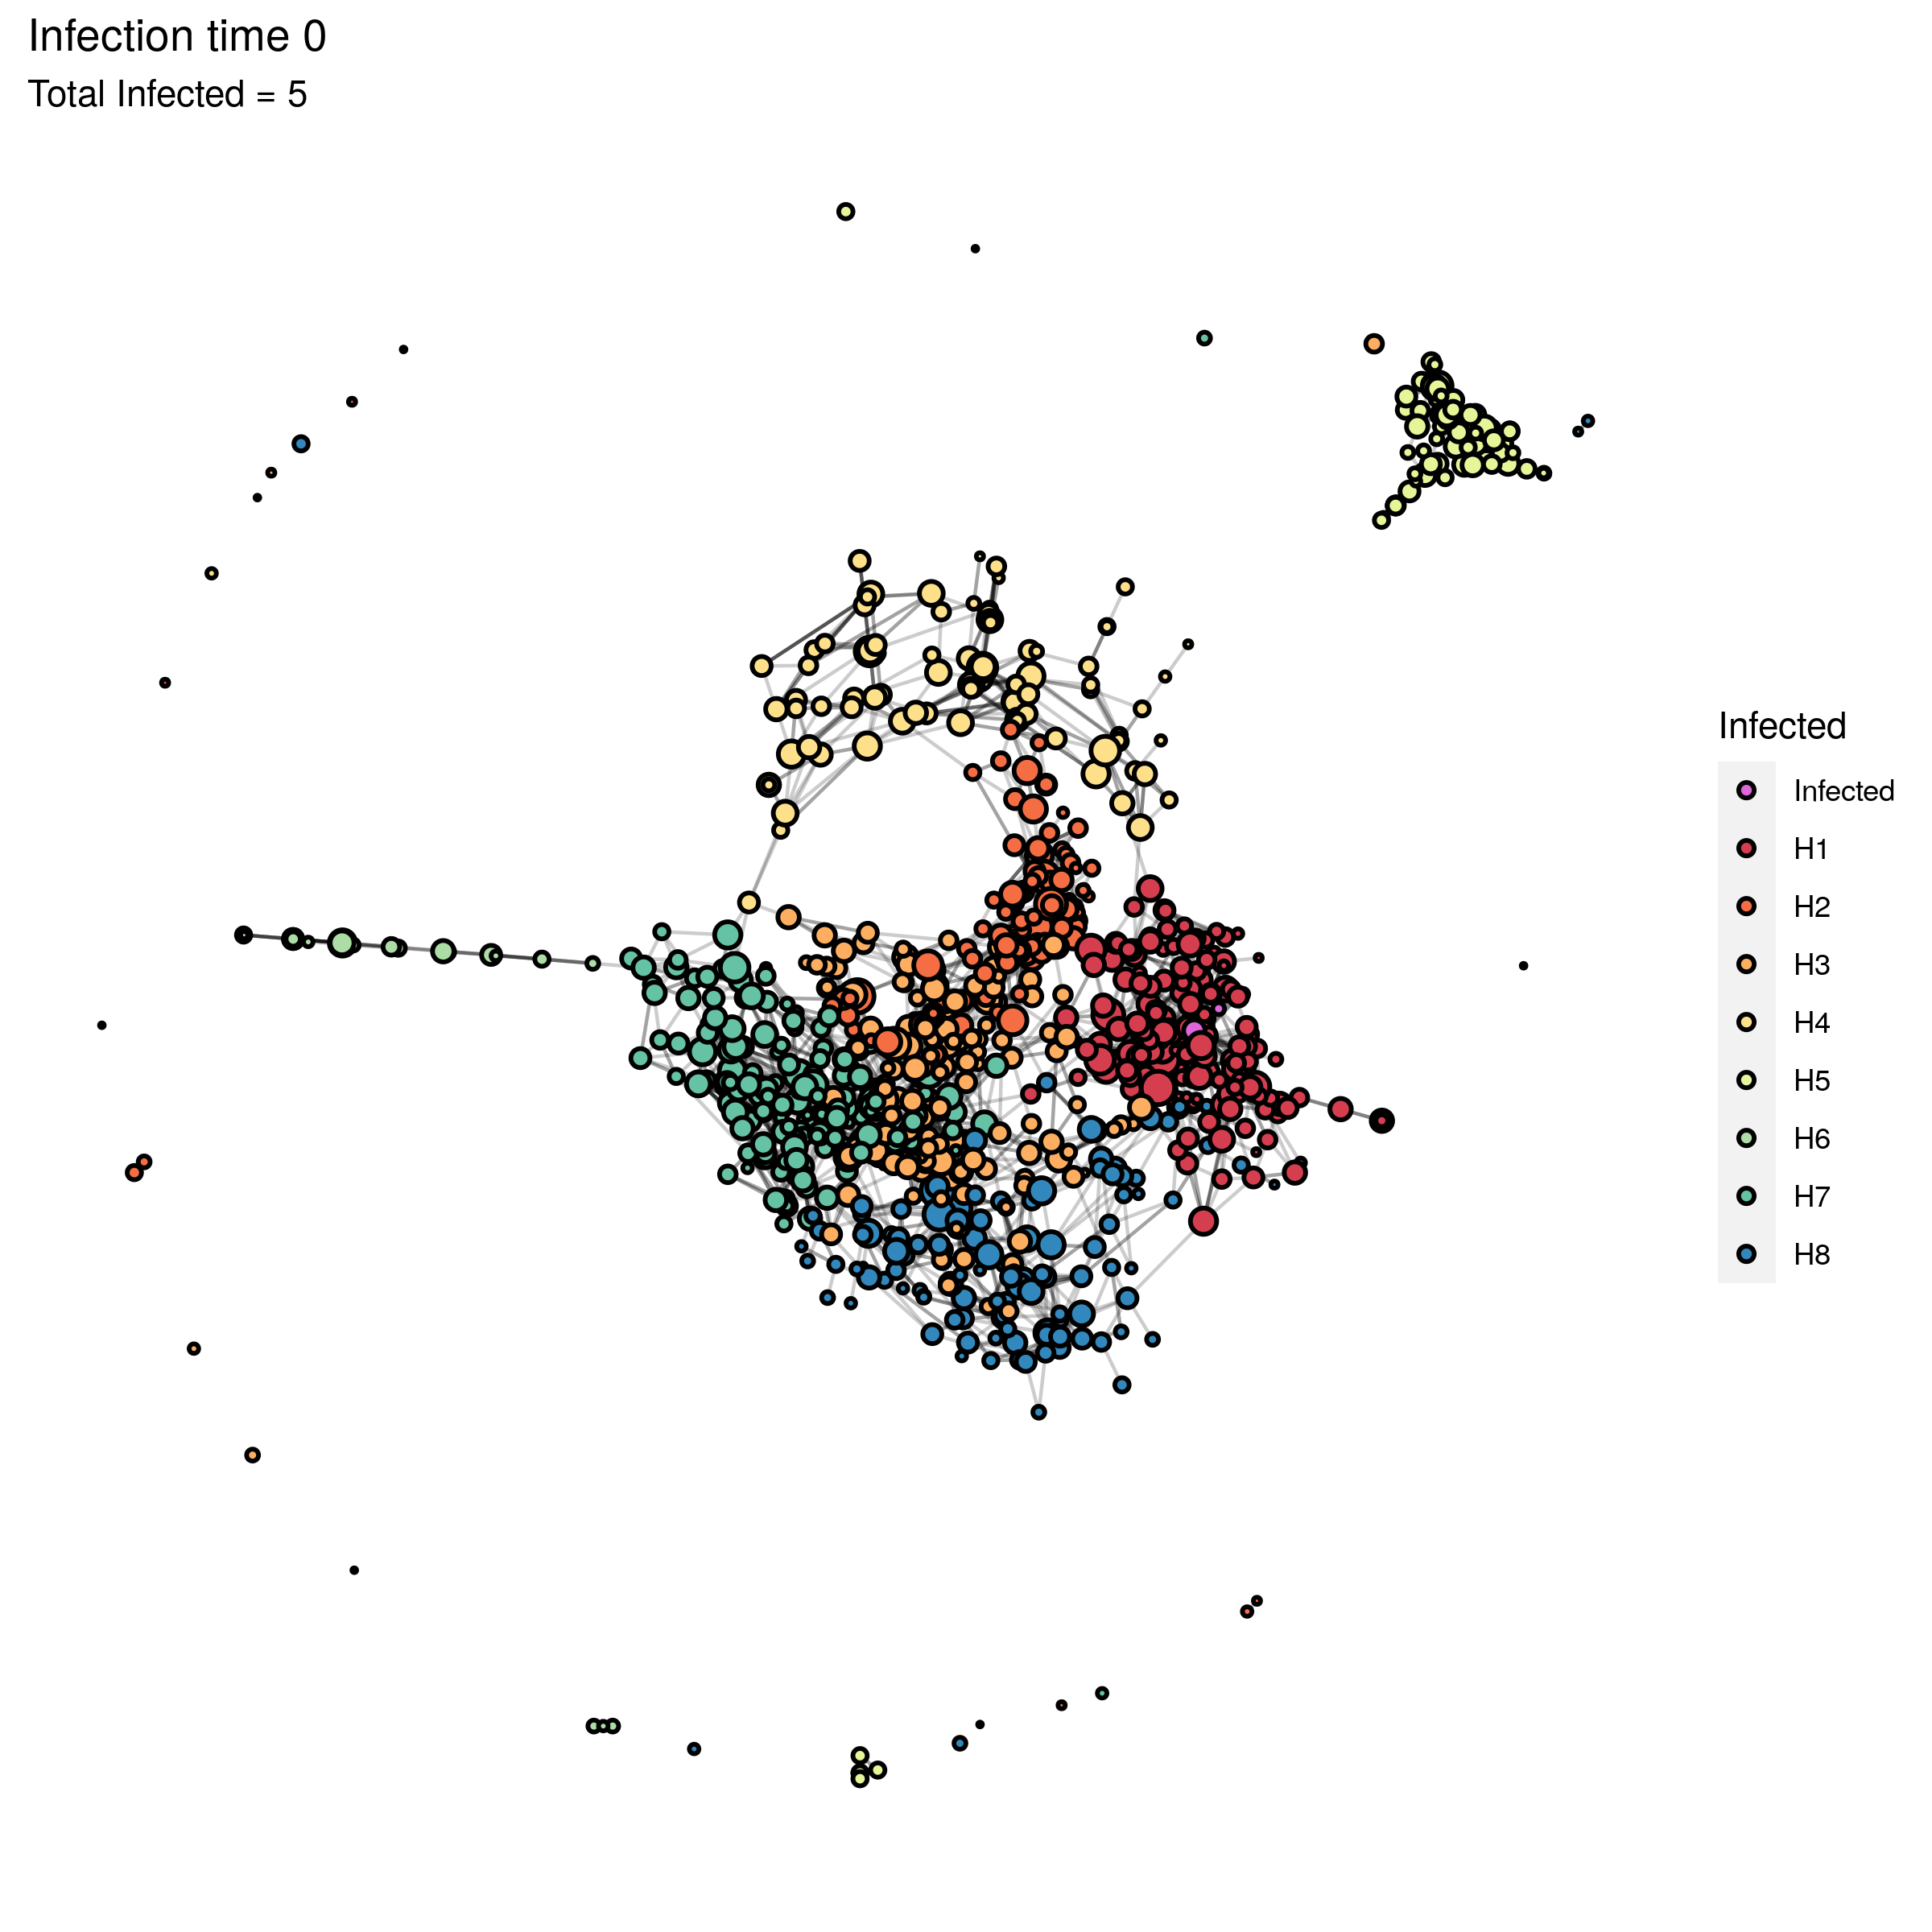
\includegraphics[width=\linewidth]{figures/Networks/Video/Graph_Infection_0_Infected___manual.png}
        \caption{a}
    \end{minipage}
    \hfill
    \begin{minipage}[b]{0.45\linewidth}
        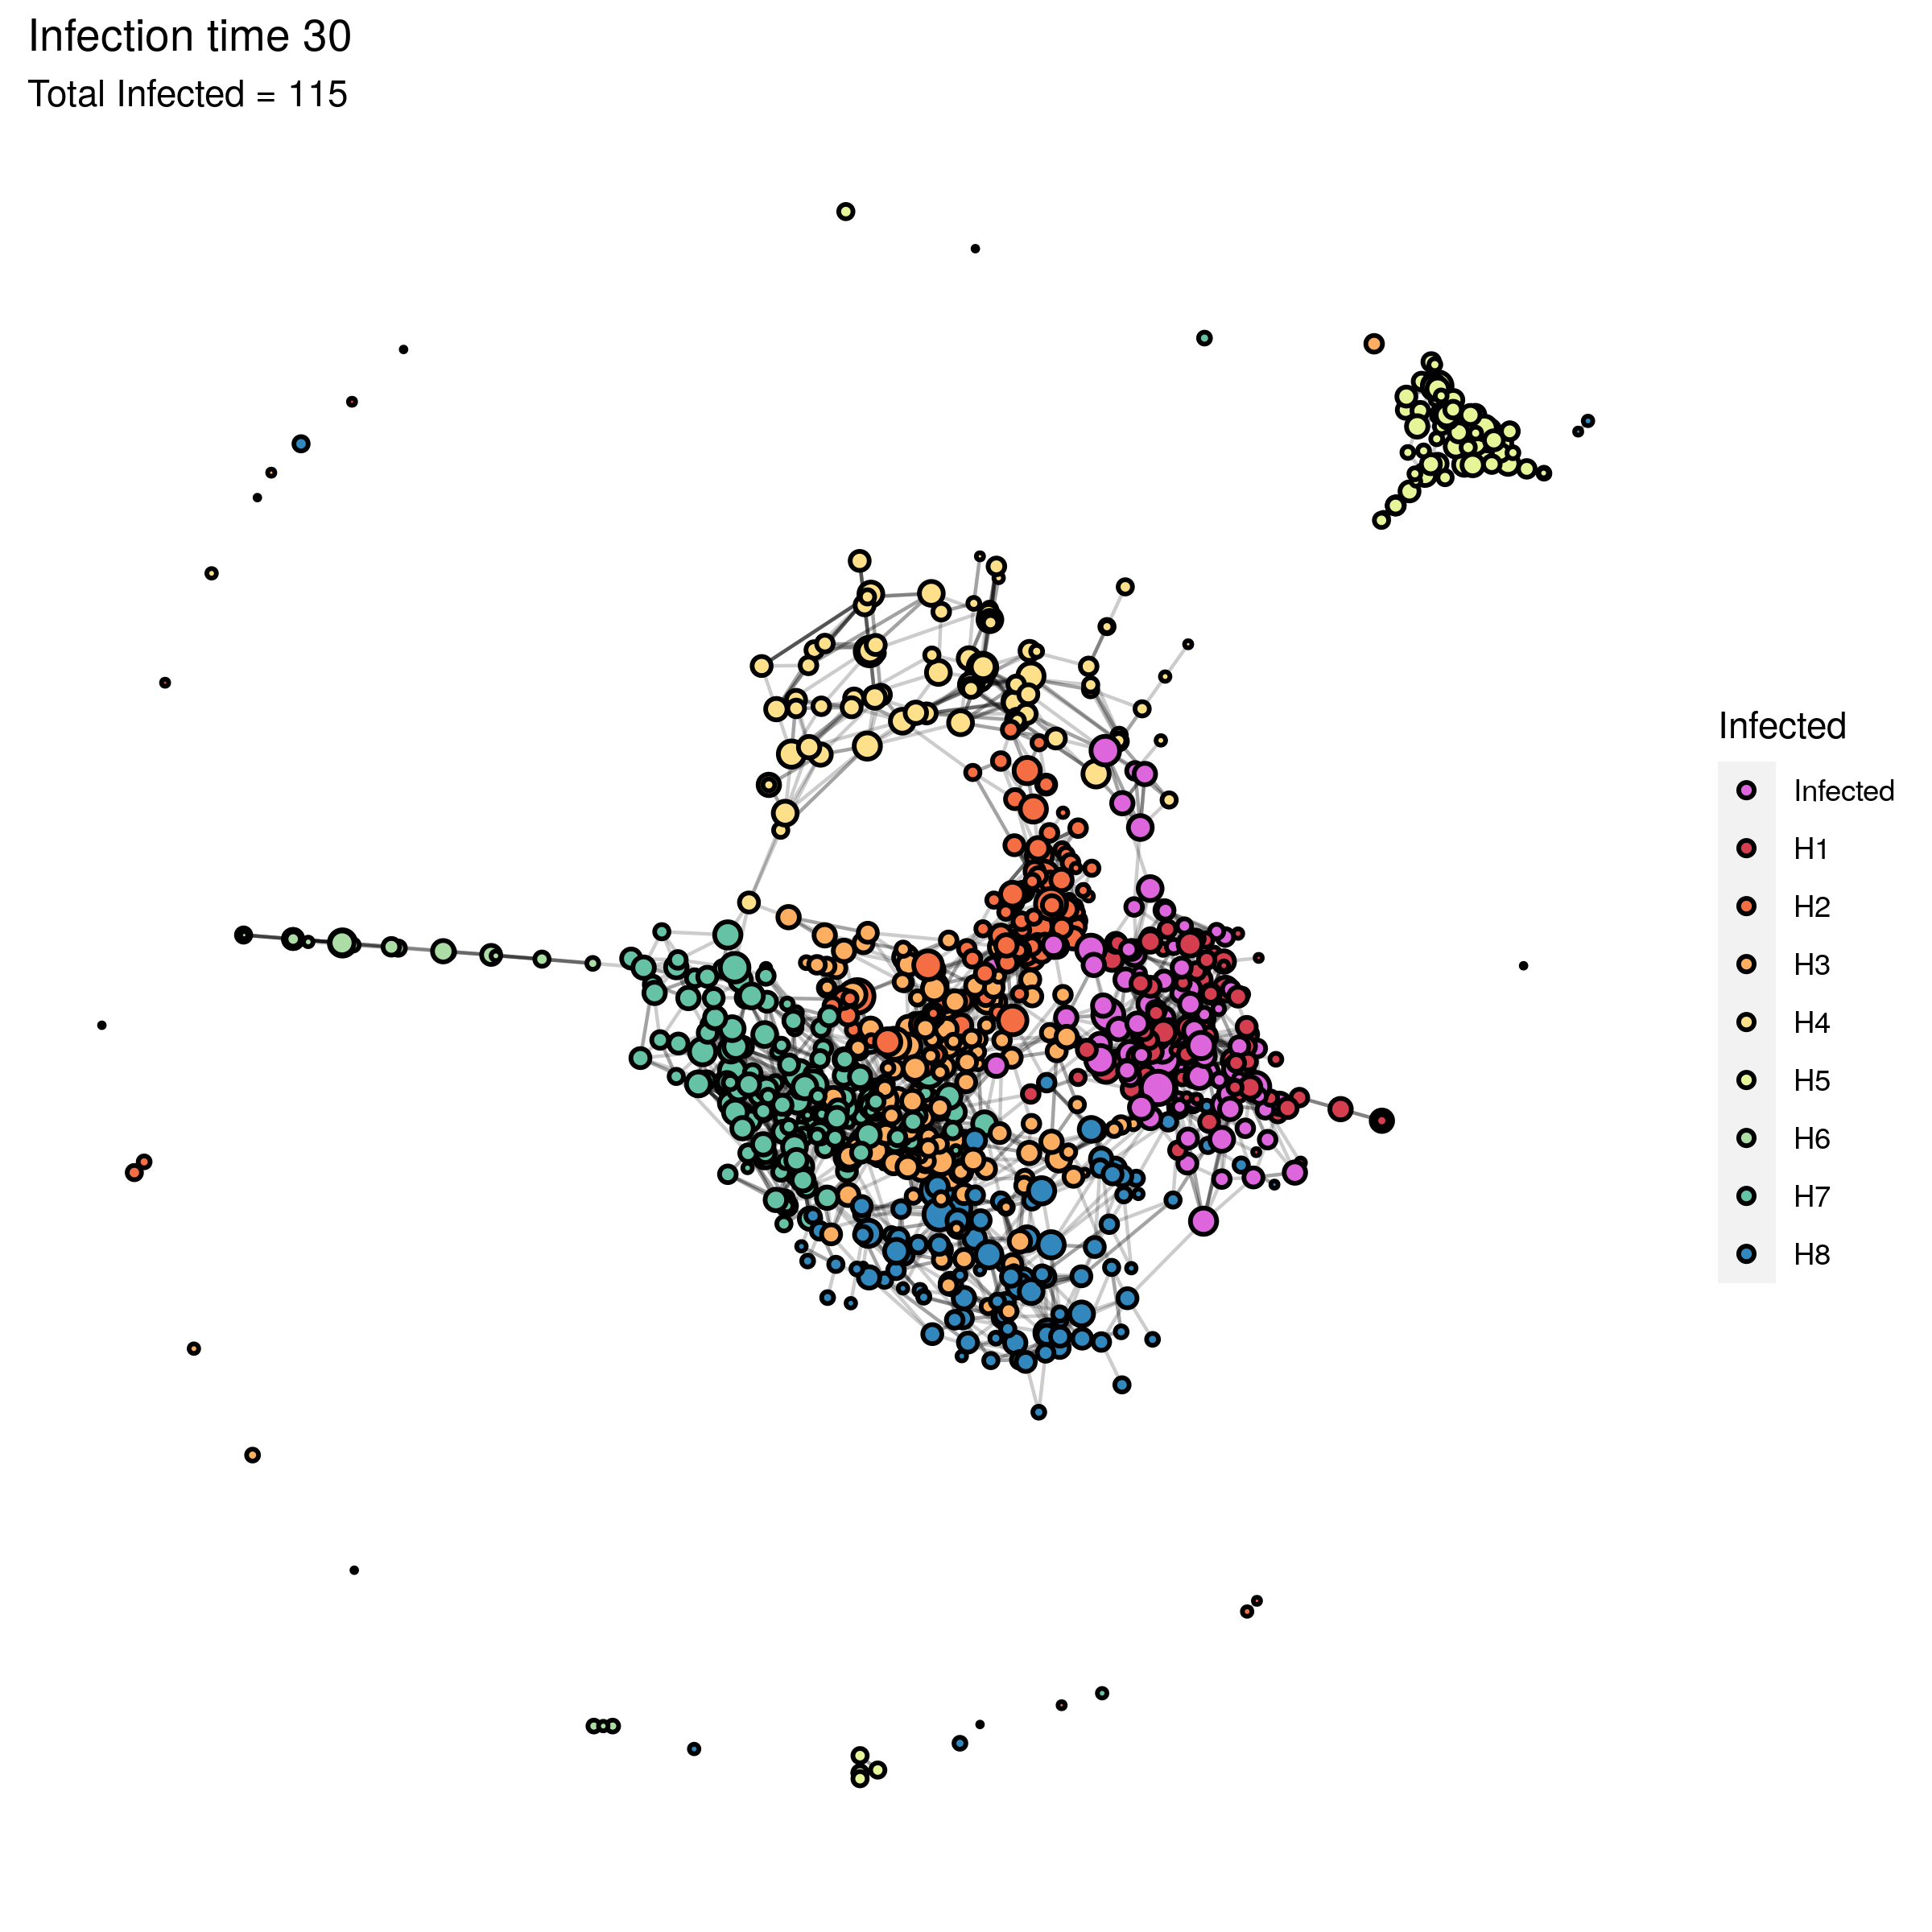
\includegraphics[width=\linewidth]{figures/Networks/Video/Graph_Infection_30_Infected___manual.png}
        \caption{b}
    \end{minipage}
    \vfill
    \begin{minipage}[b]{0.45\linewidth}
        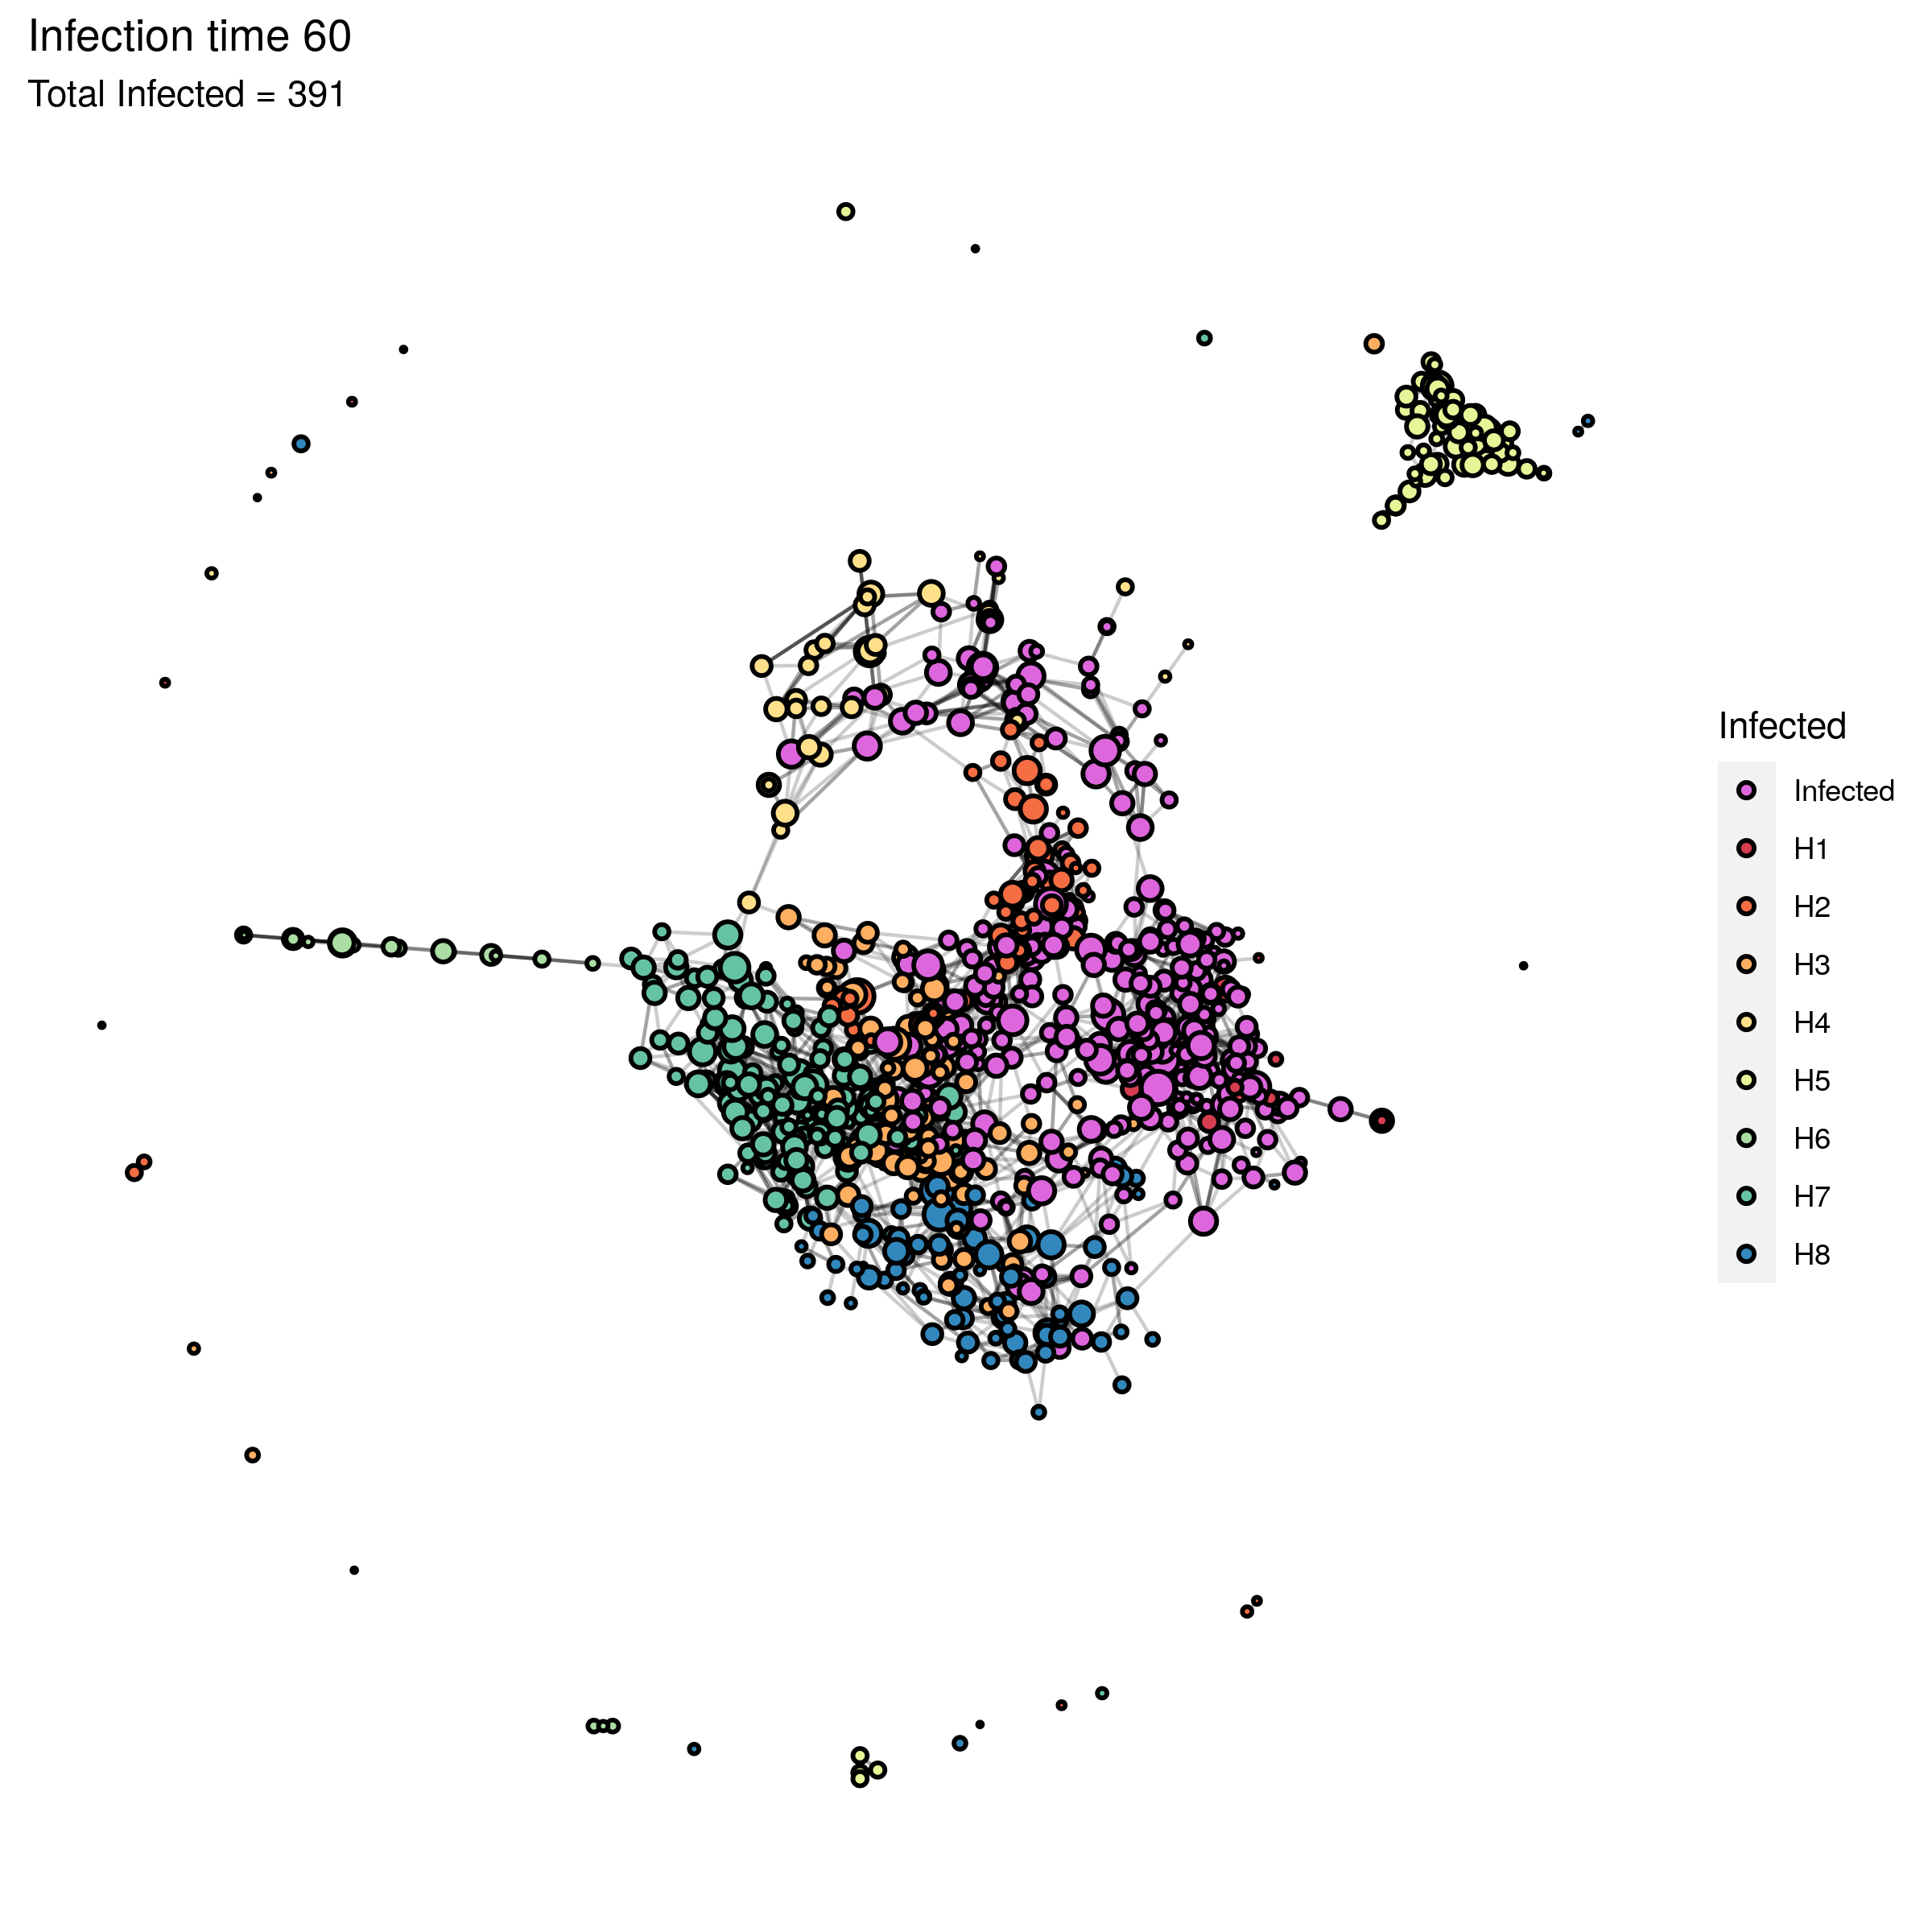
\includegraphics[width=\linewidth]{figures/Networks/Video/Graph_Infection_60_Infected___manual.png}
        \caption{c}
    \end{minipage}
    \hfill
    \begin{minipage}[b]{0.45\linewidth}
        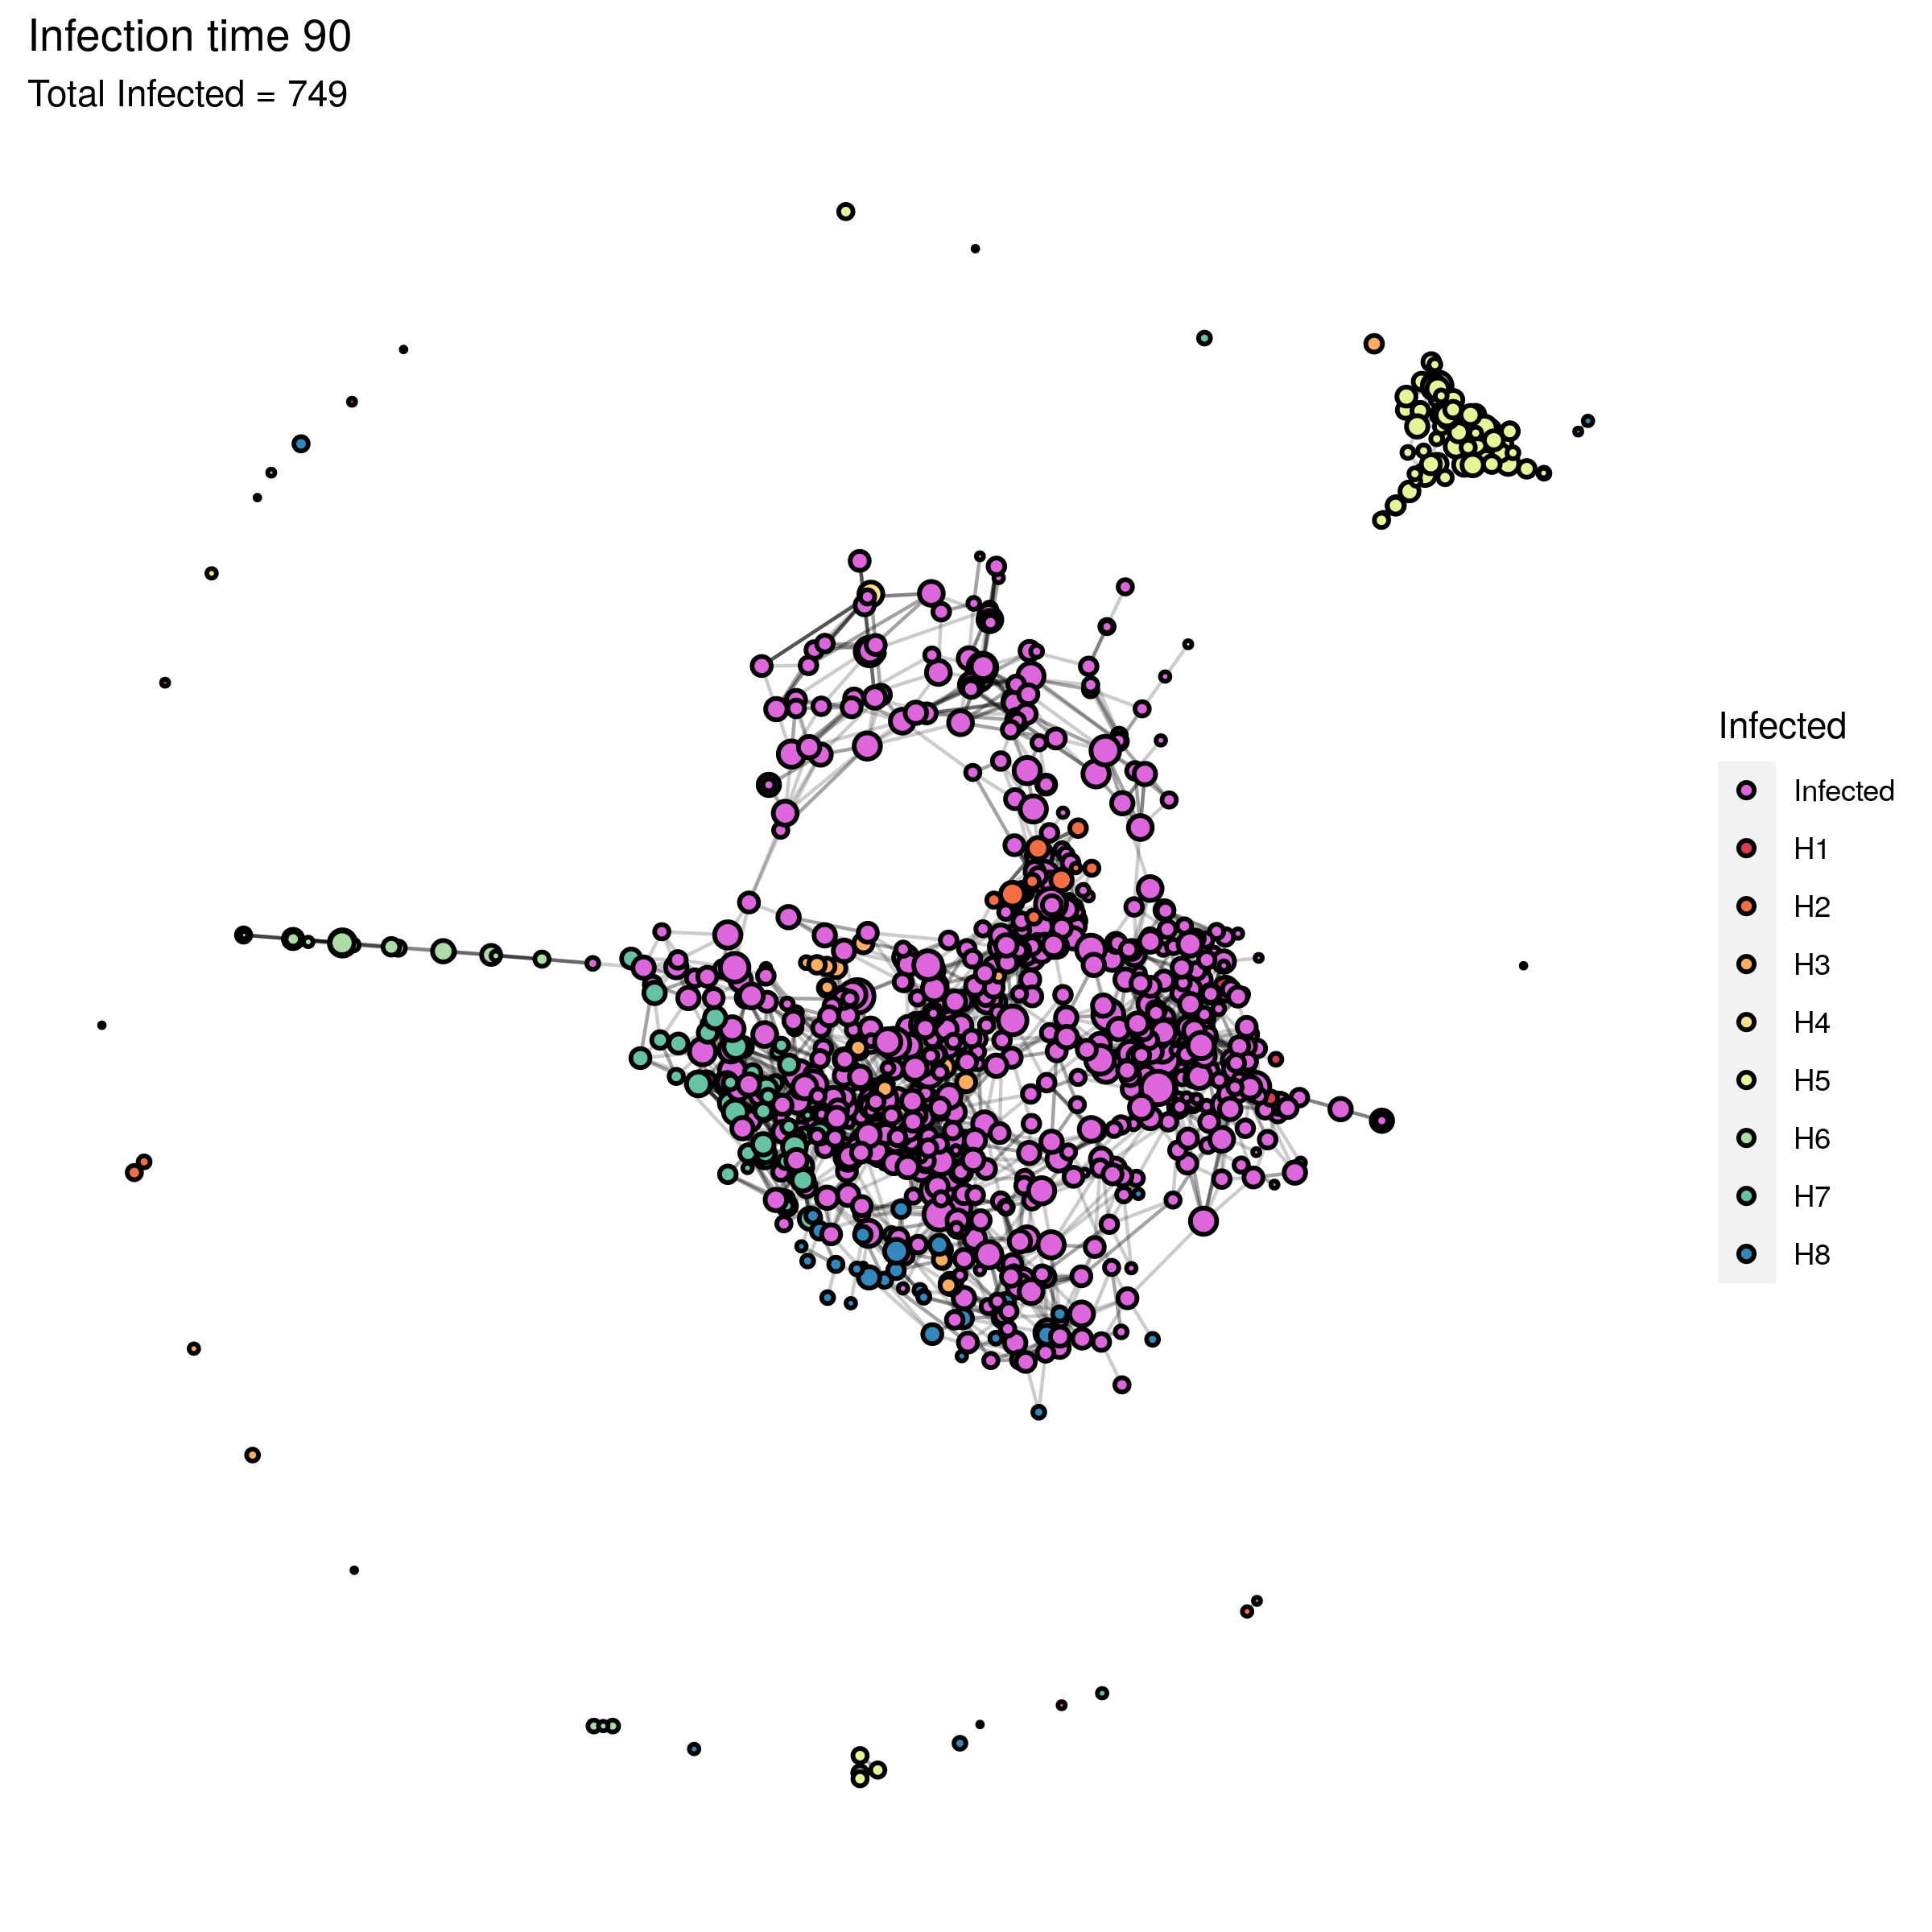
\includegraphics[width=\linewidth]{figures/Networks/Video/Graph_Infection_90_Infected___manual.png}
        \caption{d}
    \end{minipage}
    \caption{A simulation of a disease advancing through the School Network using an MDS layout. Each sub-figure represents the disease advance after (a) 0 steps with 5 random initials infected (b) 30 steps (c) 60 steps (d) 90 steps. Infected people are highlighted in violet, and each school is highlighted in a different color. The disease starts in H1 and spread to closer contacts. H5 and all isolated components are spared because is not connected and thus impossible to reach in this particular model. The complete video of the simulation can be found at \url{https://github.com/uit-hdl/mimisbrunnr/blob/main/results/network/simulation.mp4}}
    \label{fig:networkVideo}
\end{figure}


%\begin{figure}
 %   \centering
  %  \subfigure[]{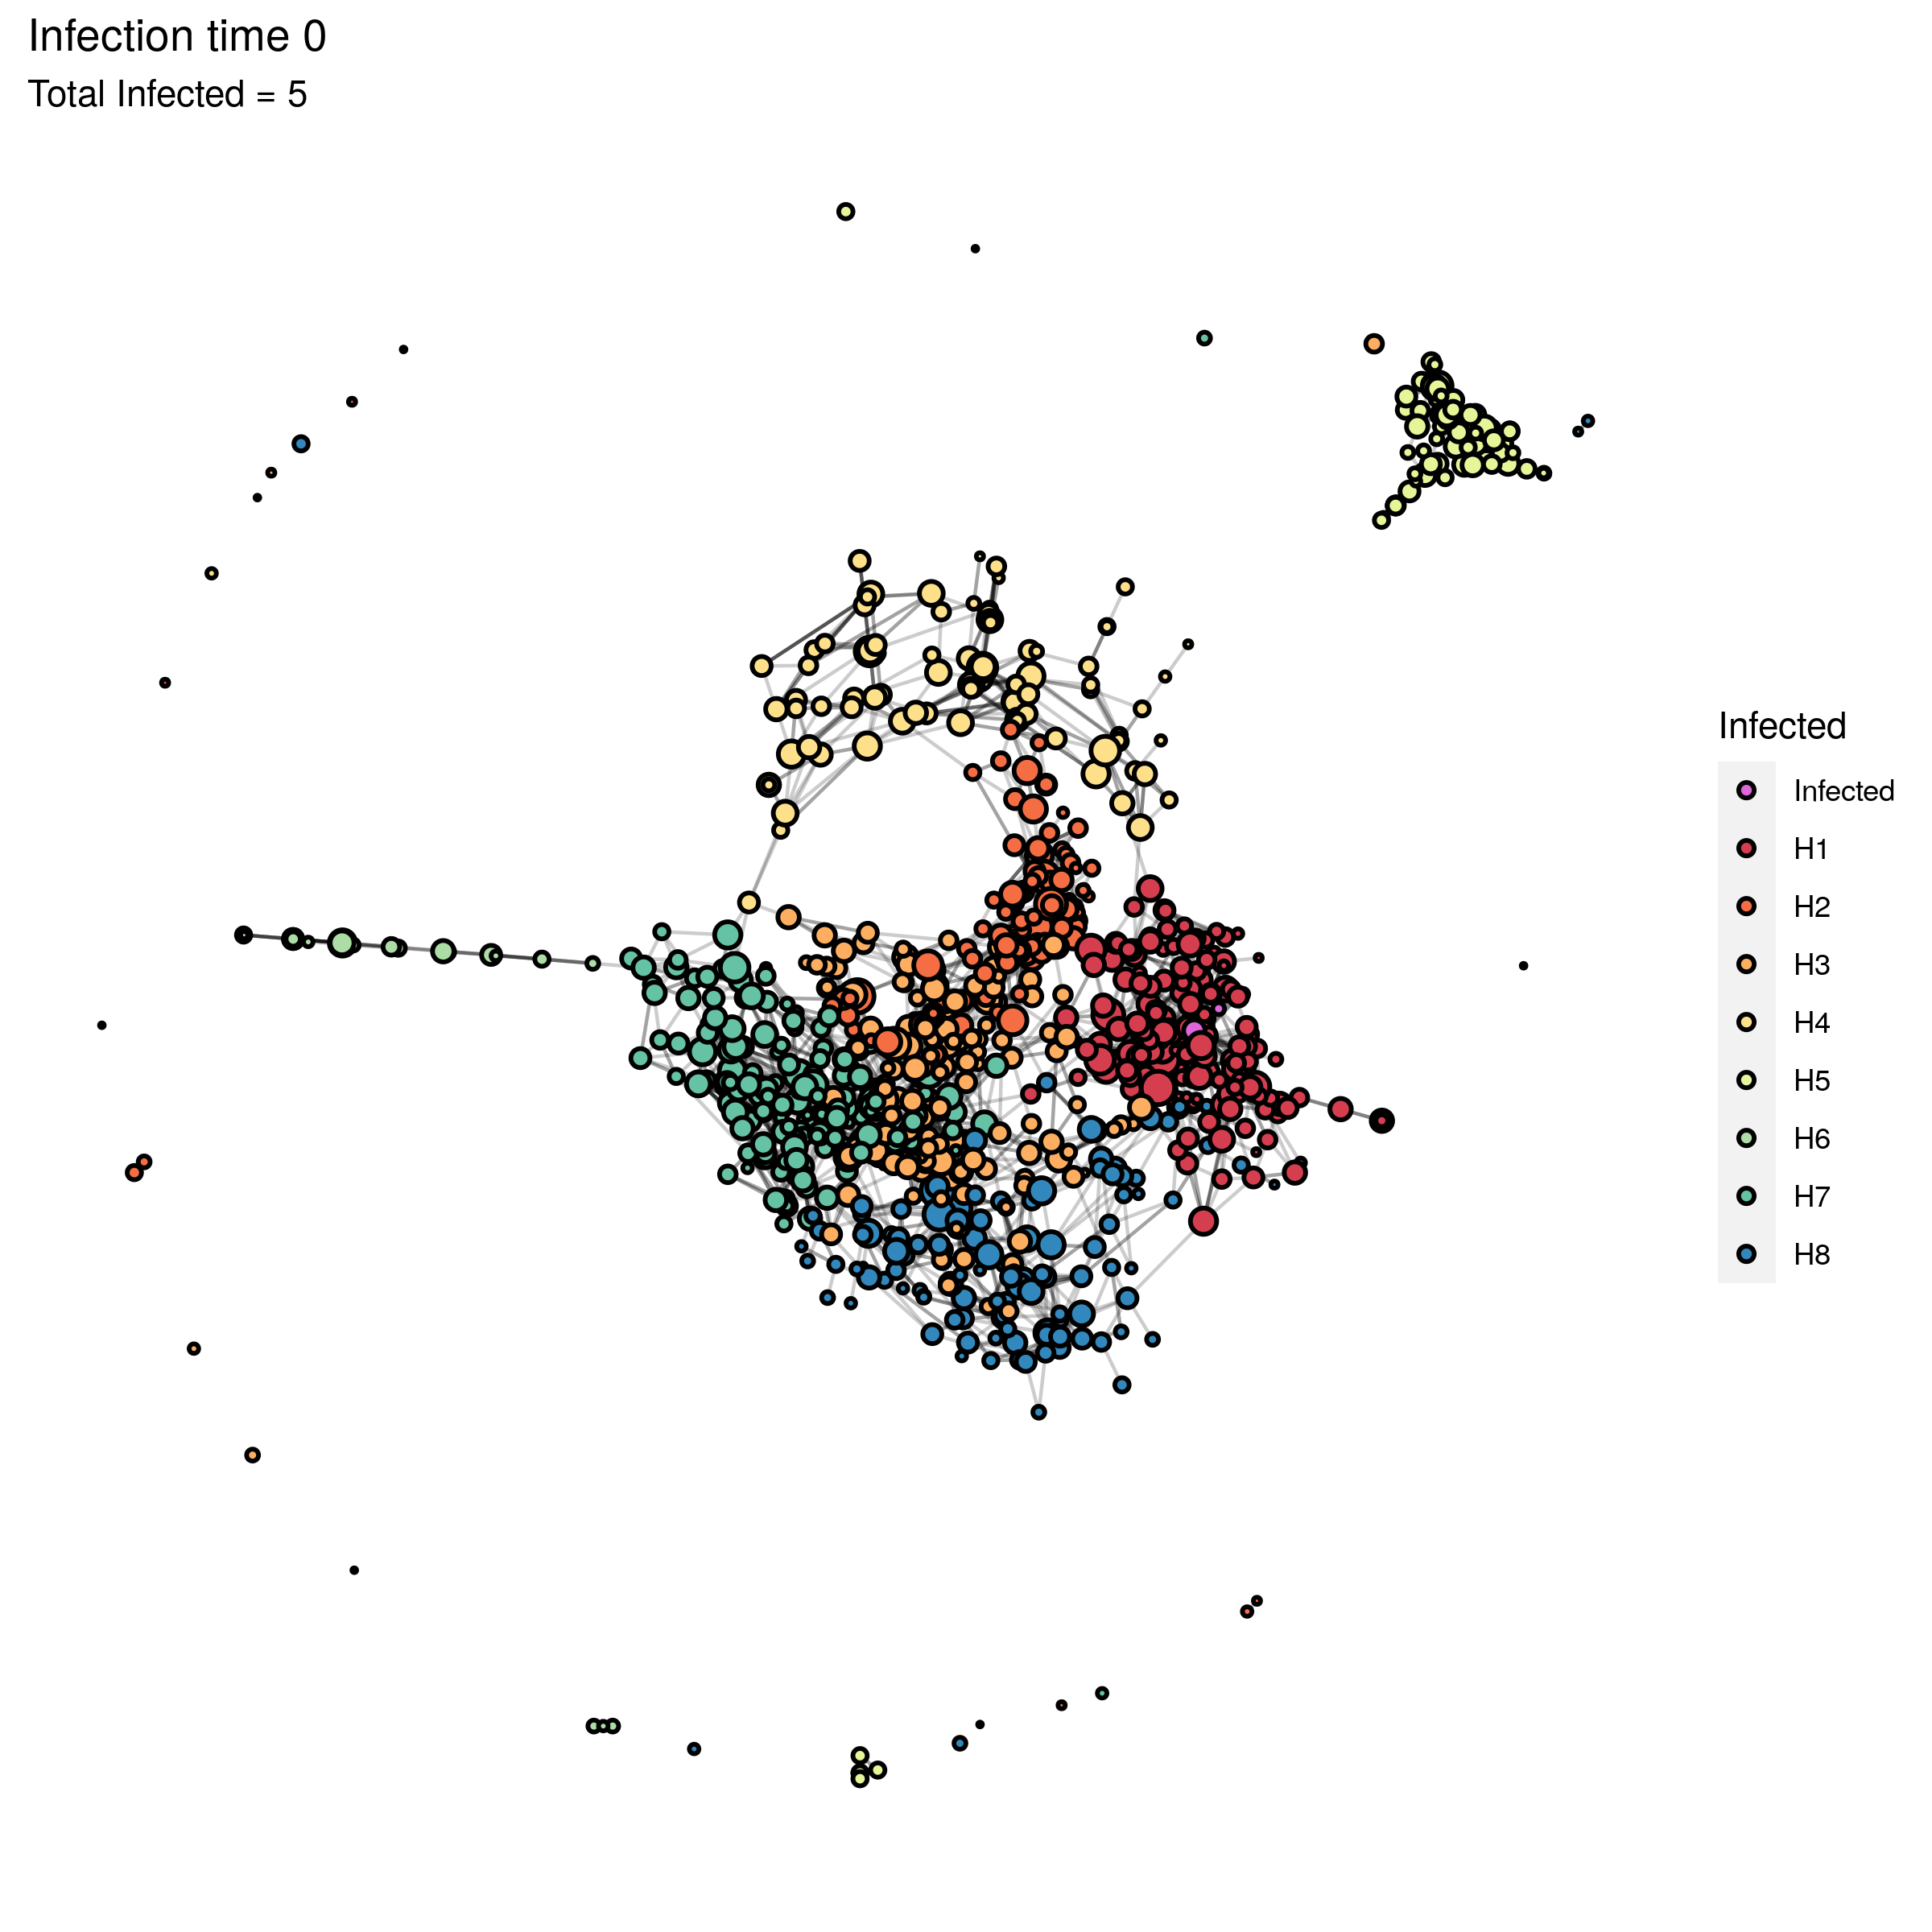
\includegraphics[width=0.45\textwidth]{figures/Networks/Video/Graph_Infection_0_Infected___manual.png}} 
   % \subfigure[]{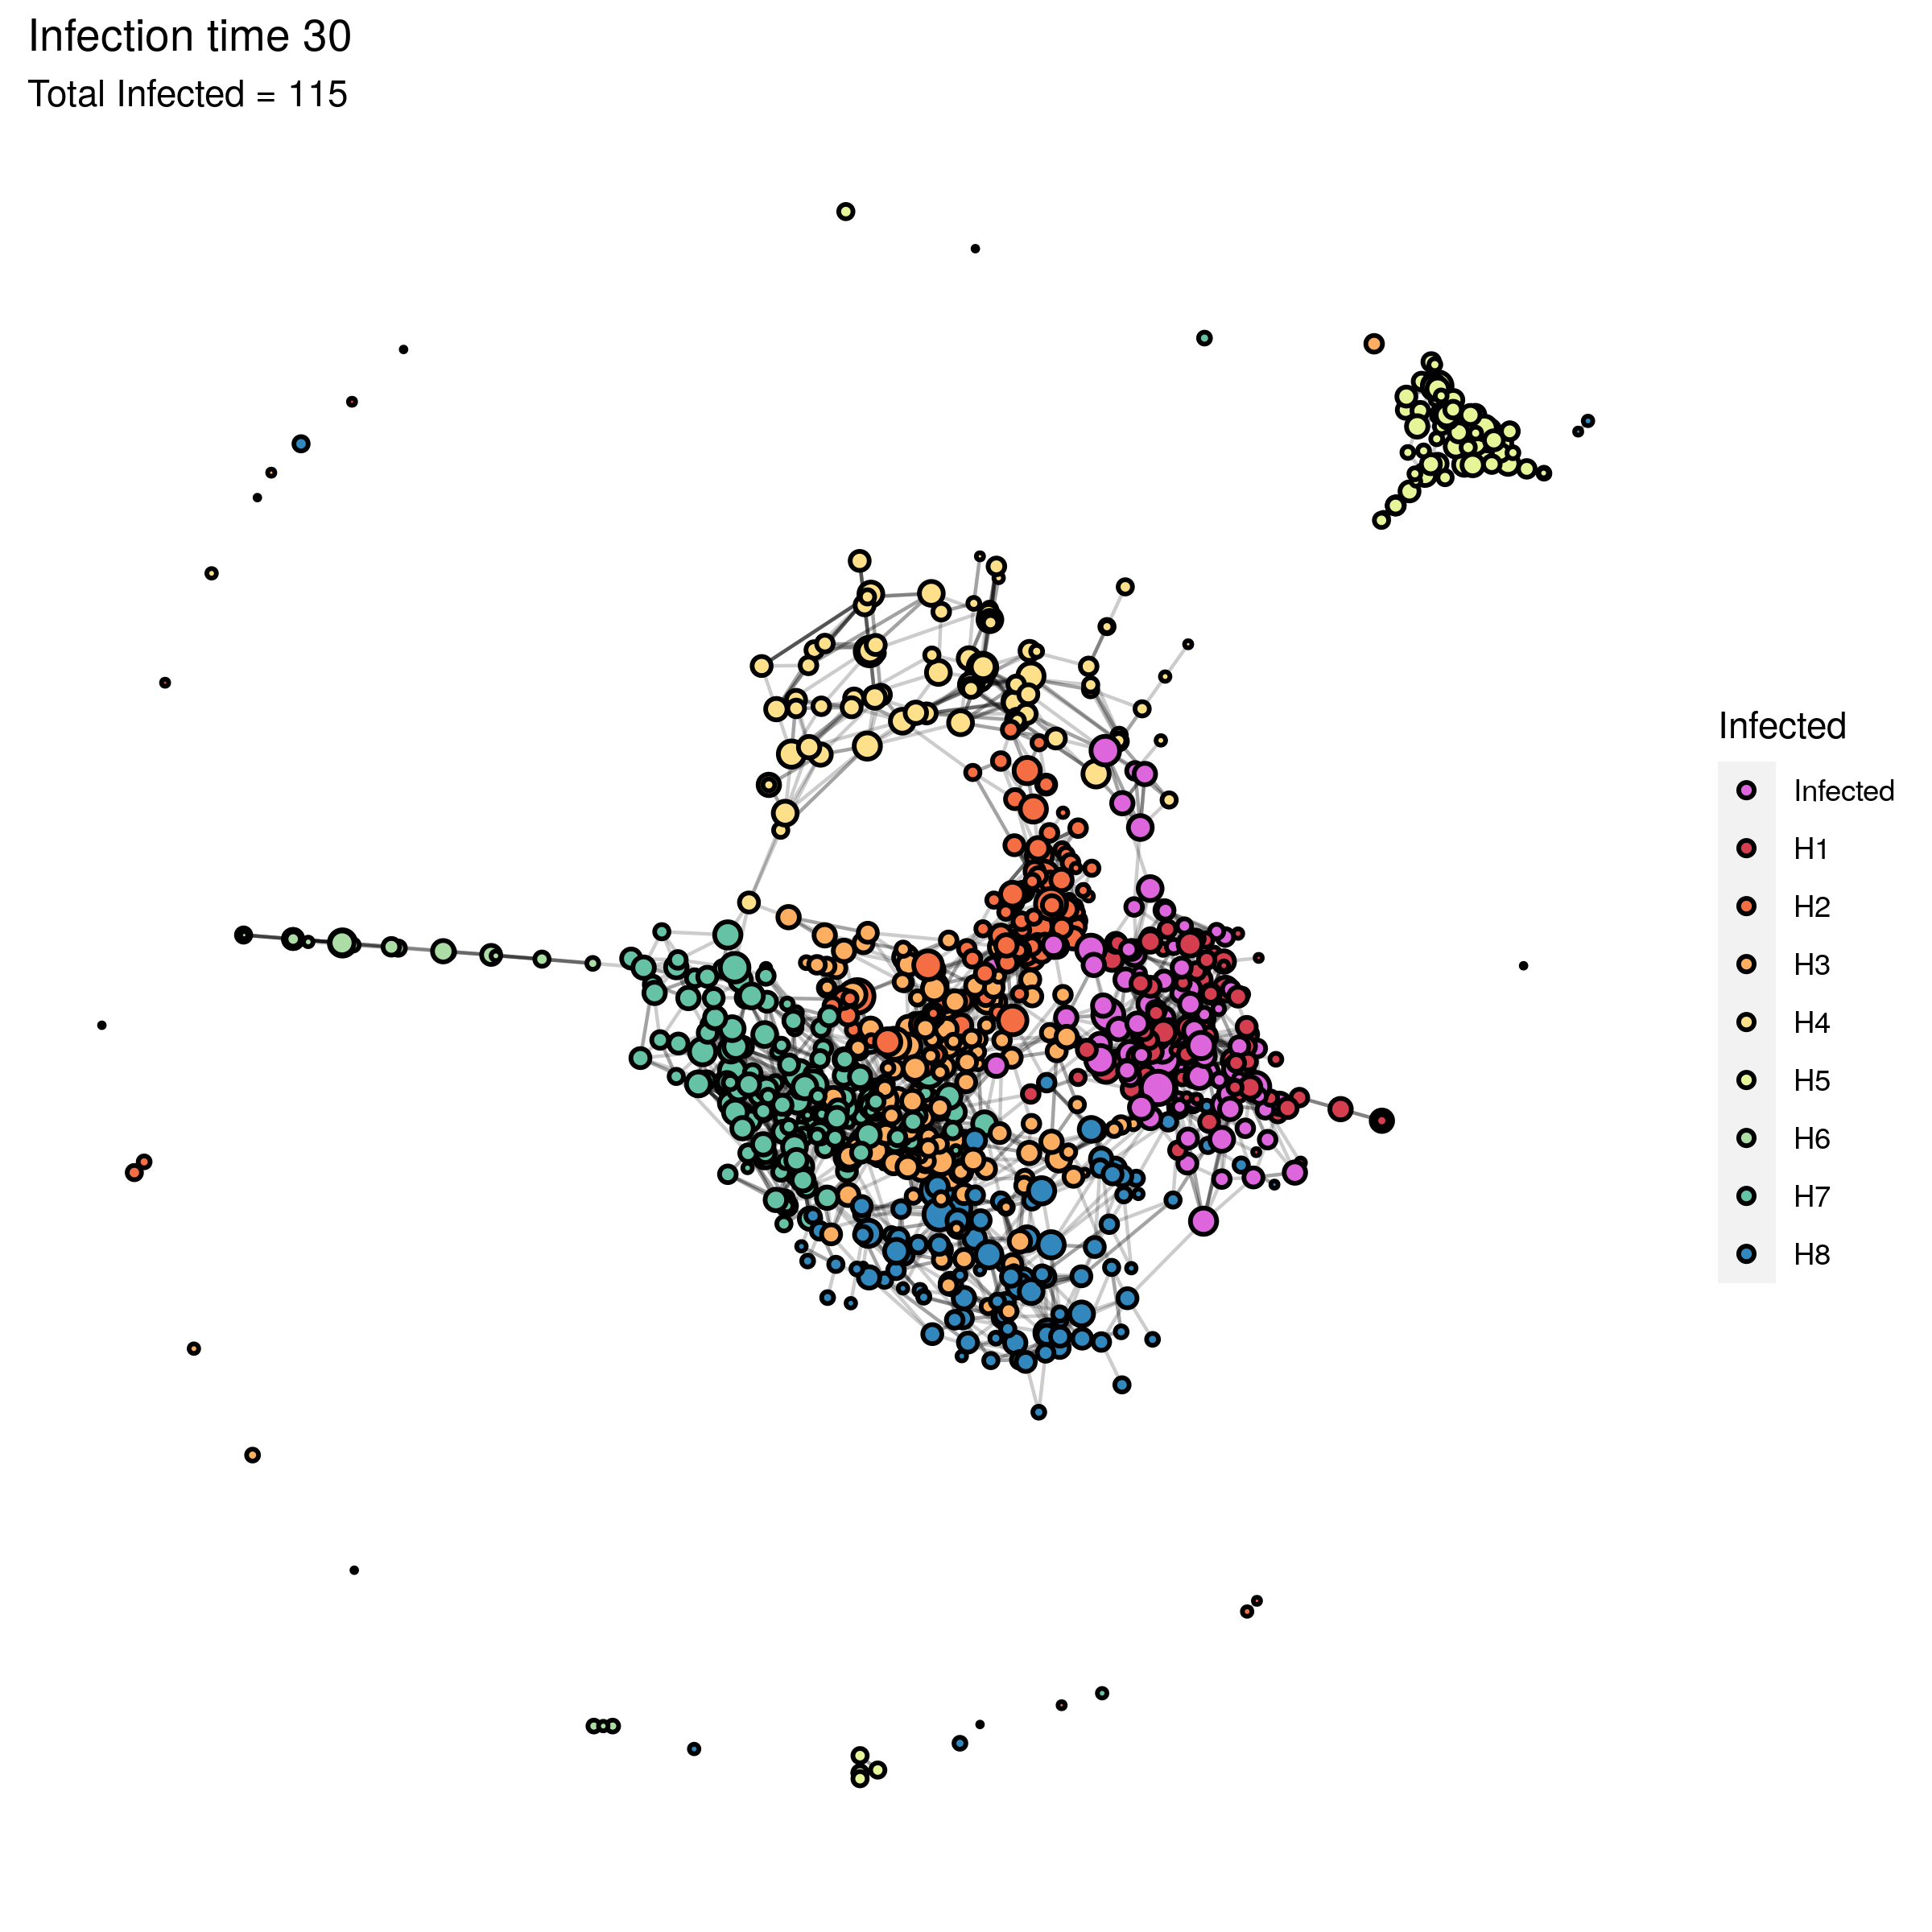
\includegraphics[width=0.45\textwidth]{figures/Networks/Video/Graph_Infection_30_Infected___manual.png}} 
    %\subfigure[]{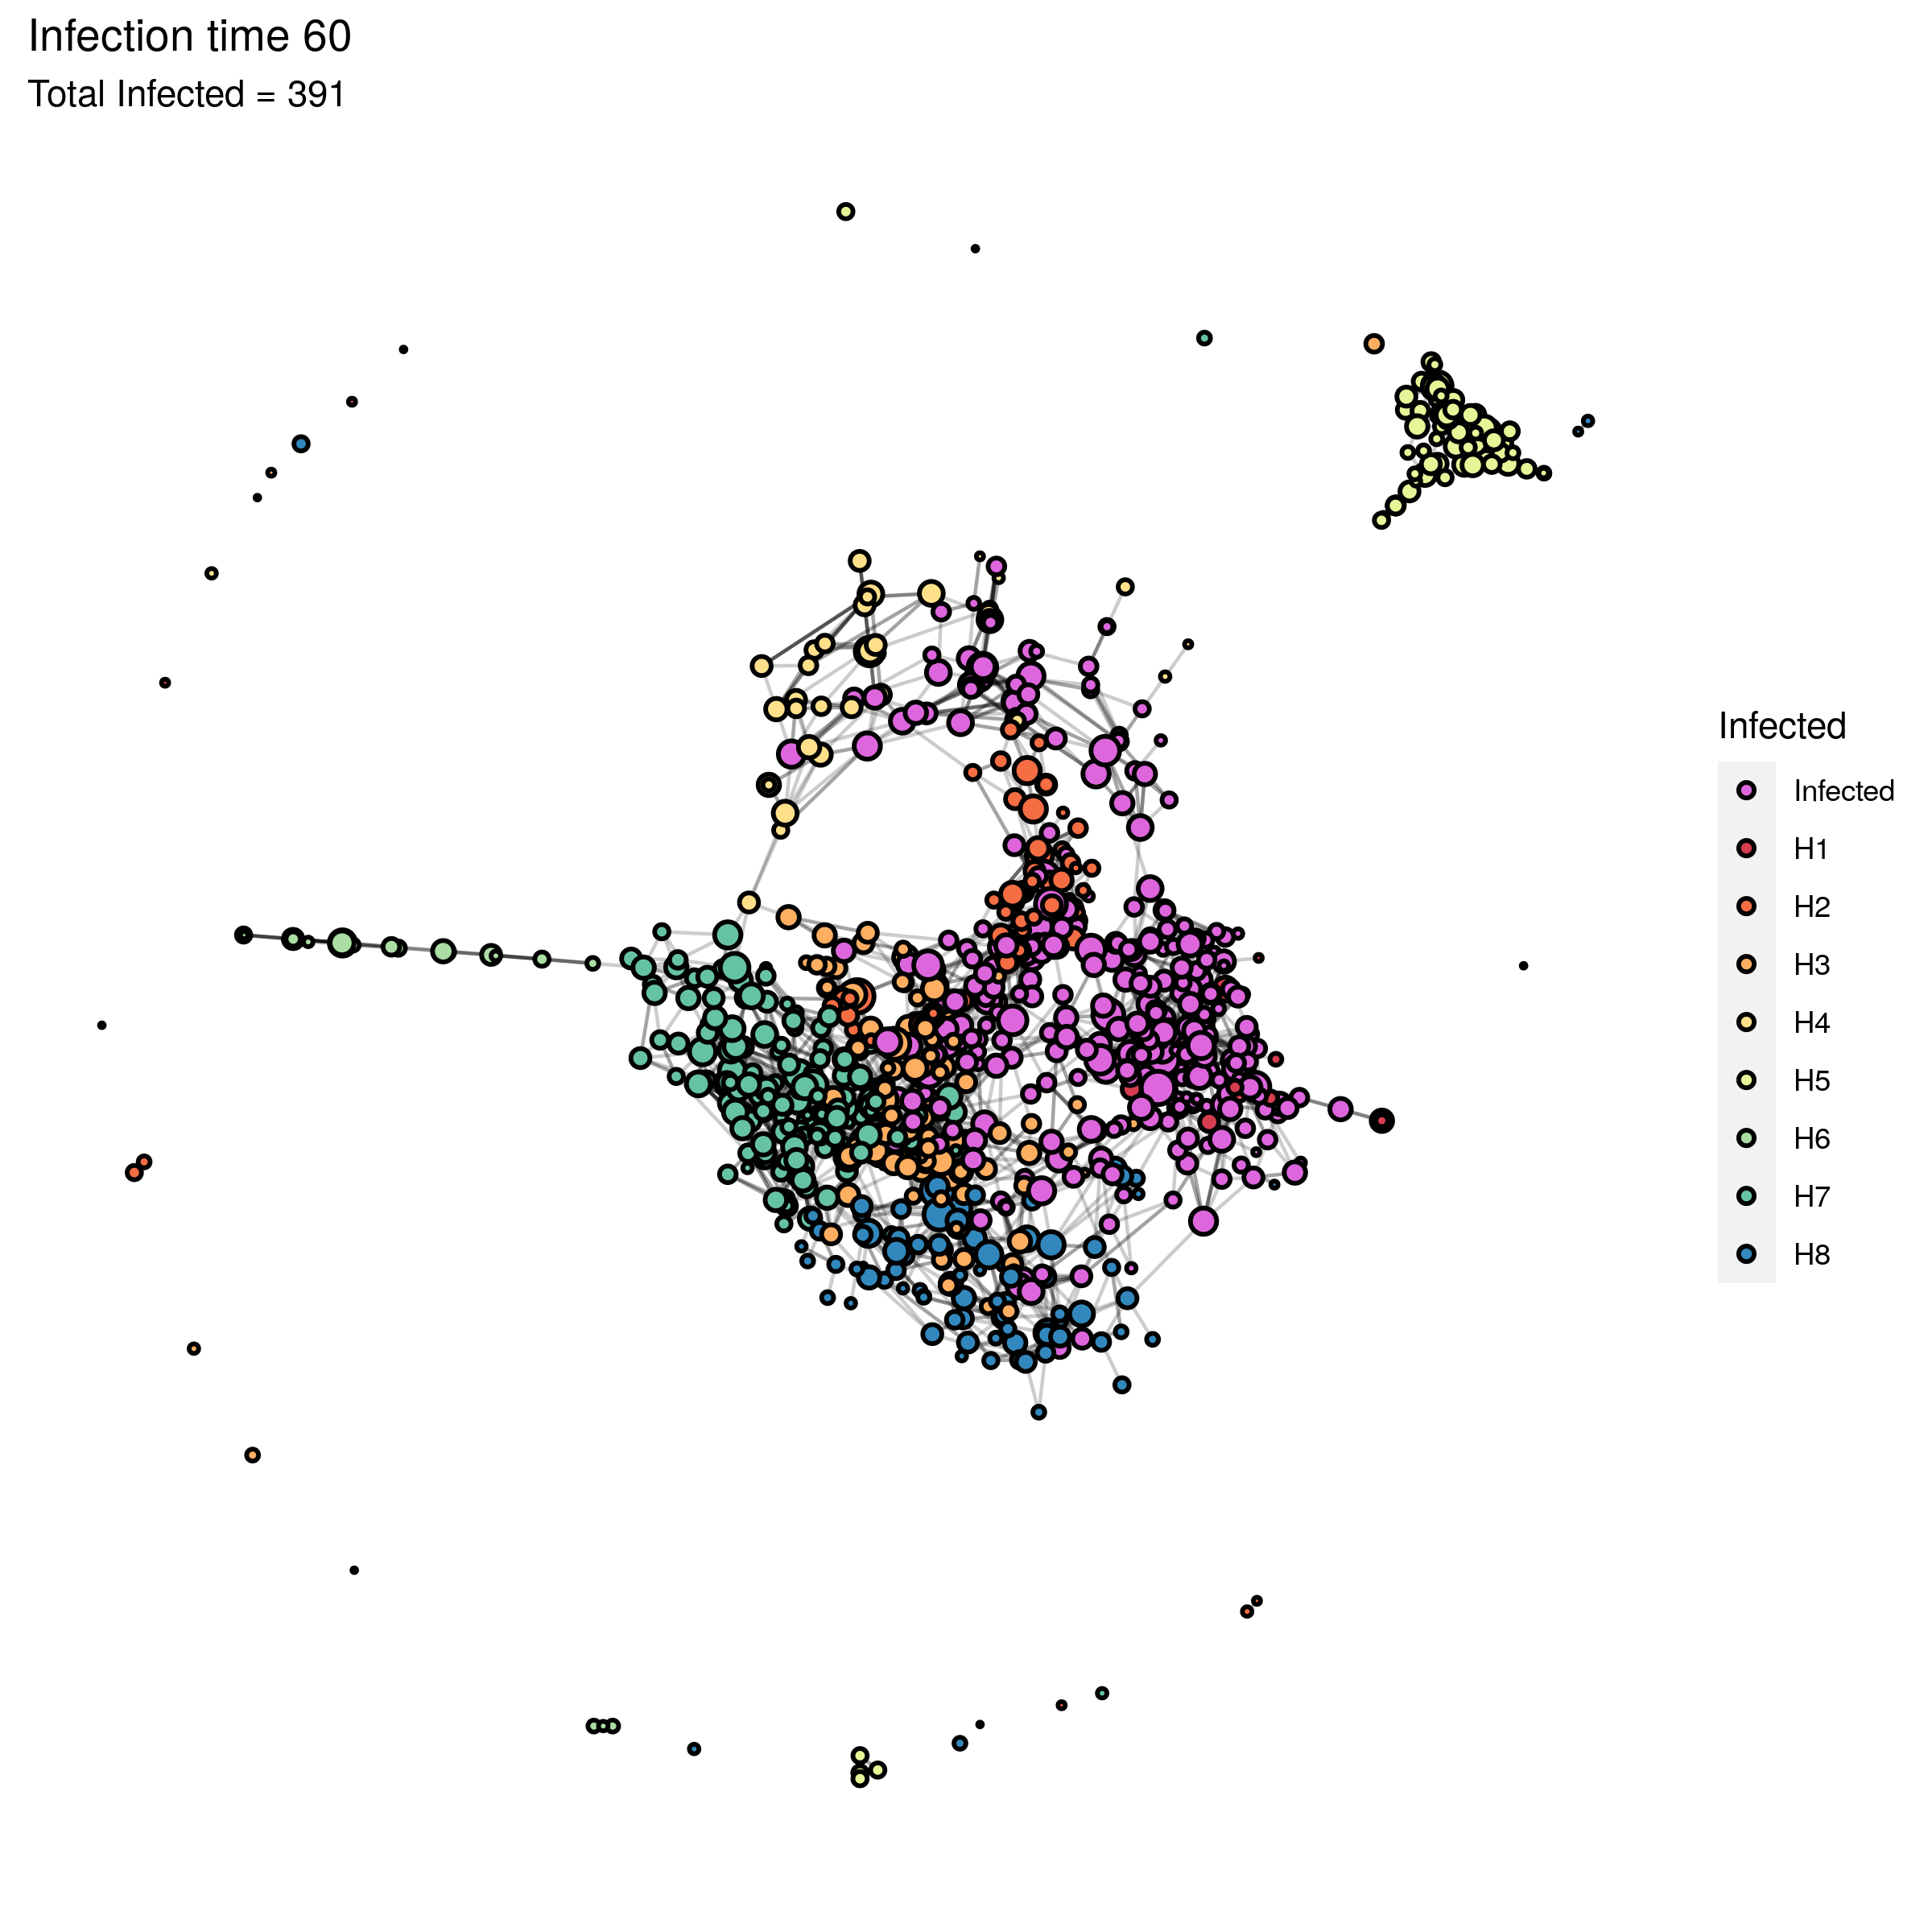
\includegraphics[width=0.45\textwidth]{figures/Networks/Video/Graph_Infection_60_Infected___manual.png}}
    %\subfigure[]{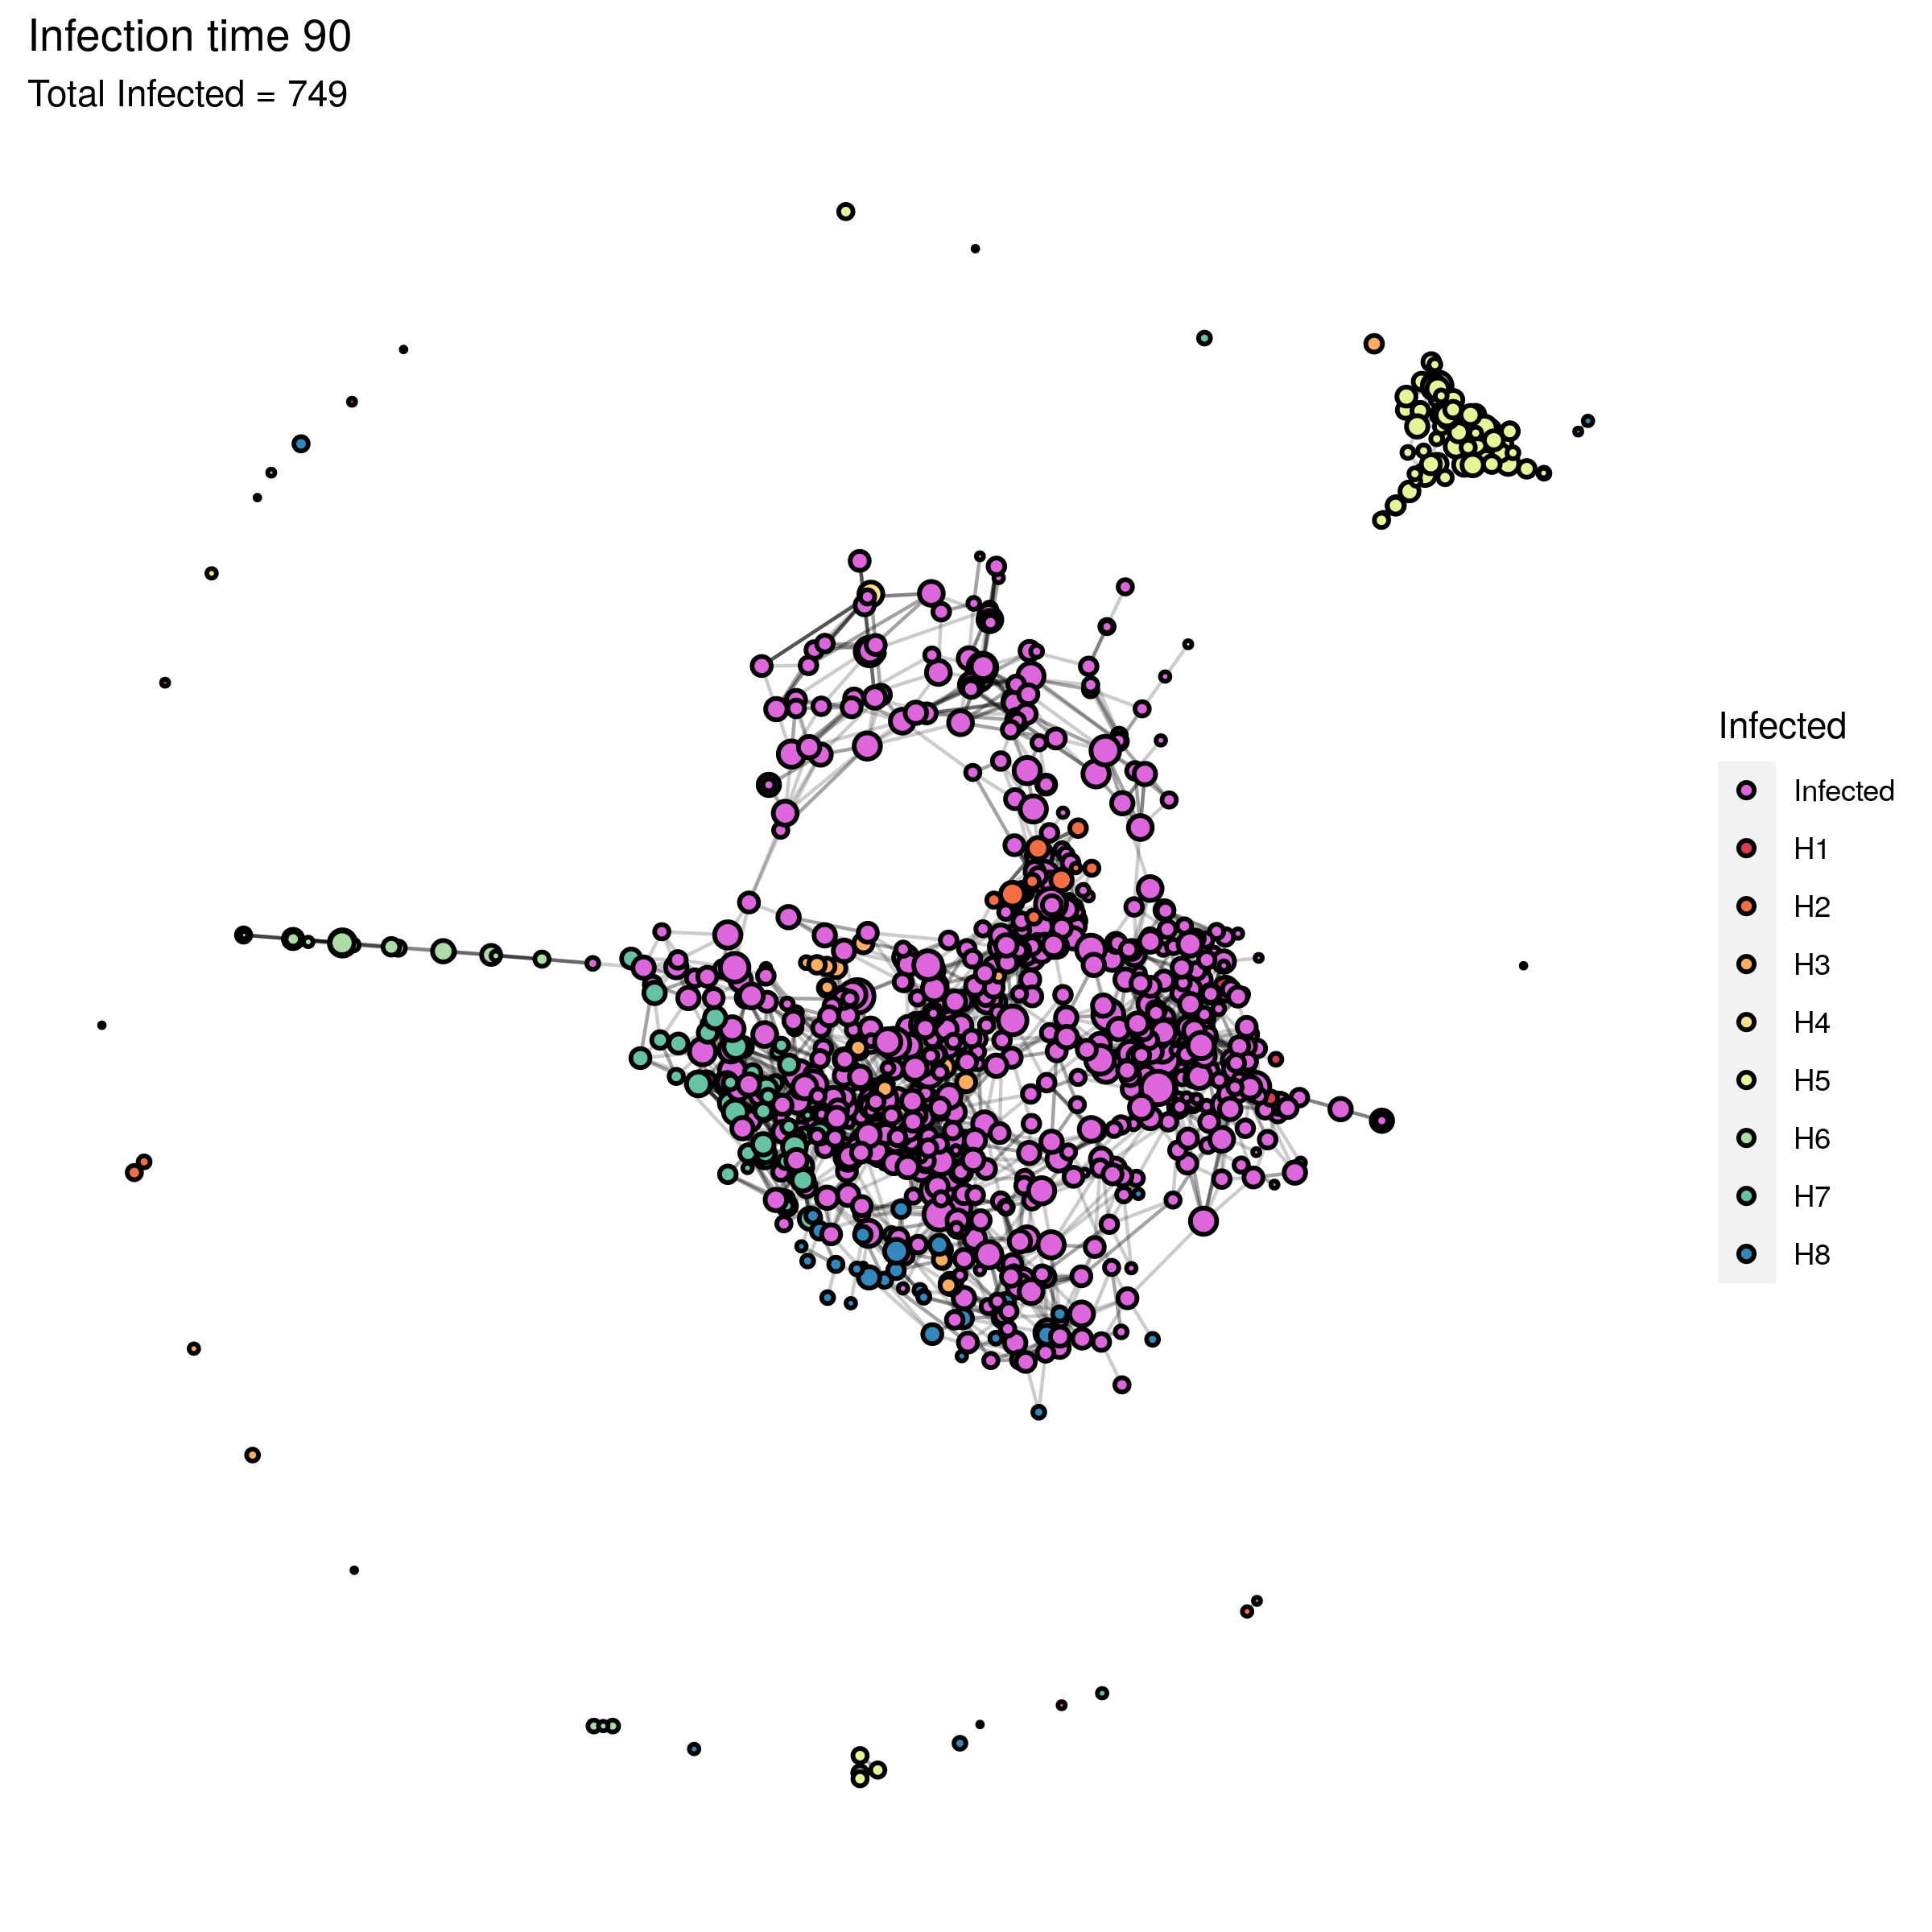
\includegraphics[width=0.45\textwidth]{figures/Networks/Video/Graph_Infection_90_Infected___manual.png}}
    %\caption{A simulation of a disease advancing through the School Network using a MDS layout. Each sub-figure represent the disease advance after (a) 0 steps (b) 30 steps (c) 60 steps (d) 90 steps. Infected people are highlighted in violet, each school is highlighted in a different color. The disease start in H1 and spread to closer contacts. H5 is spared because is not connected and thus impossible to reach in this particular model. The complete video of the simulation can be found at \url{https://github.com/uit-hdl/mimisbrunnr/blob/main/results/network/simulation.mp4}}
    %\label{fig:networkVideo}
%\end{figure}

\section{Final}

You can learn more about how to draw a network in Paper F \ref{chapter:chapterListPapers}. Furthermore, all the code which generates figures and tables for this thesis is available in our GitHub repository. Several other good and free resources exist online %https://bdpedigo.github.io/networks-course/plotting_networks.html


% Introduction to Staph
%*****************************************
\chapter{Staphylococcus aureus}\label{ch:staph}
%*****************************************

\section{Introduction}

The word "Staphilus" derives from the Greek "σταφυλόκοκκος", composed of "staphylé" meaning bundle, and "coccus" meaning grape. This refers to their bundle of grapes-like arrangement. "Aureus" comes from Latin origin meaning golden, which is the golden-orange characteristic color of this bacteria as it is rich in carotenoid pigments. \gls{staph} was discovered in 1880 by Alexander Ogston who noticed a formation of bacteria in pus during a procedure he was performing. Wounds caused by \gls{staph} infections were fatal for most patients until the 1940s when it was discovered that penicillin could cure such infections. But unfortunately, by the end of the century, the penicillin resistance strain became widespread. This led to the development of methicillin, which was a better option to treat infections caused by the bacteria. However, again, the bacteria evolved to be antibiotic resistant, called \gls{mrsa}. Once this strain was characteristic of the hospital, but today is widespread in the general population.

Nearly 30\% of humans are carriers of \textit{S. Aureus} which are usually present in the skin and the upper respiratory tract. Males have a higher prevalence, but the bacteria can also be found specifically in the lower reproductive tracts of females. Under normal circumstances the bacteria are harmless, but they can cause a wide range of diseases which will be discussed later, ranging from minor skin diseases such as pimples or follicles the most common ones, to life-threatening ones such as pneumonia, endocarditis, and sepsis. Is in the top five most common intrahospital infections and is the most common cause of wound infection after surgery, causing around 500.000 hospital infections in the US alone, of which 10\% end up in death related to such infections.

In the forthcoming chapter, the primary attributes of this bacterium will be described, alongside a comparative description of its likeness to other pathogens and to what makes it unique.

\section{Microbiology introduction}

There are 5 pathogenic agents for humans. Four of them are microbes (viruses, bacteria, fungi, and parasites) and the last one is called prions.

\begin{itemize}

\item 
\textbf{Prions} are misfolded proteins capable of making other well-structured proteins also misfold, triggering a chain reaction in the organism. Generally, they provoke neurodegenerative diseases in humans and are transmitted via ingestion of animal corpses that already contain the protein. A well-known example of this in cattle would be \gls{bse}, commonly known as mad cow disease, which spreads to humans in the form of \gls{vcjd}, which is mainly caused by feeding ground animal carcasses to cows. There's no effective treatment for prion diseases and the only prevention against it is to avoid contaminated meat. Only the complete denaturation of the protein can destroy a prion.

\item 
\textbf{Viruses} characterize for needed a host to inject their genetic profile to reproduce. Once this is done, the viral genetic material merges with the host DNA, forcing the replicating mechanism of DNA to create more copies of the virus. There is a huge range of diseases caused by viruses such as the common cold or AIDS, with also many types of methods of transmission. Treatments generally consist of either a vaccine that teaches the immune system how to recognize the virus before it replicates too much, or antiviral drugs that drop fake DNA blocks that get incorporated into the virus genome preventing further replication.

Neither prions nor viruses are considered to be alive, which is why we refer to viruses as particles and not microbes.

\item 
\textbf{Fungal} infections are likely to be transmitted via inhalation, ingestion, or direct surface contact; and rarely directly from person to person. Diagnosis of fungal infection is relativity easy as only 4 non-opportunist fungi are known to be able to actively infect humans; but in contrast, mycosis is a difficult disease to heal. These diseases typically present as a form of lung or skin infection and range in all possible levels of severity. Mycotoxicosis makes a reference to getting poisoned by fungal toxins, and mycetismus is a reference to getting poisoned by eating the fungi themselves. Neither case has anything to do with infections.


\item 
\textbf{Parasite} may refer to two kinds of organisms. One causes parasitic infections, and the other simply feeds from the host resources but does not necessarily cause diseases or discomfort. Many parasites are not microscopic despite being classified as microbes. Parasites are generally transmitted via contact with parasite reservoirs such as food, water, insects, animals, or feces.

The three main types of parasites are Protozoa single-celled parasites which can multiply inside the host, Helminths which are worms, and Ectoparasites which typically live outside of the host such as lice, fleas, or mosquitos. Common diseases caused by parasites are malaria, Changas, toxoplasmosis, acanthamoebiasis, or trichomoniasis. Symptoms of parasitic infections can include diarrhea, fever, fatigue, weight loss, and skin rashes. Treatment for parasites can involve medications such as antiparasitic drugs or antibiotics.

\item 
\textbf{Bacteria} are usually single-cell organisms. \textit{S. Aureus} generally behaves as a commensal bacteria in the skin and upper respiratory tract body doing no harm, but under certain circumstances, it can become a pathogenic bacteria. Let's explore further the characteristics of bacteria and review the \textit{S. Aureus} in context.


\end{itemize}

\subsection{Prokaryote and Eucaryote}

Prokaryotes are unicellular organisms that lack a nucleus encasing the genetic material and membrane-bound organelles. Their genetic material is a circular DNA molecule located in a region called the nucleoid. They are generally smaller in size and have simple structures compared to eukaryotes. However, they have both a cell wall and a cell membrane. This cell wall is made of peptidoglycan. Prokaryotes are unable to perform cellular respiration and don't have any cytoskeleton. \textit{S. Aureus} belongs to this category. 


Eukaryotes, on the other hand, are more complex organisms that have a nucleus enclosing genetic material and various membrane-bound organelles, such as mitochondria, endoplasmic reticulum, Golgi apparatus, and lysosomes. Their genetic material consists of several linear DNA strands contained within the nucleus. They can be unicellular or multicellular organisms. They have a cell membrane, but not necessarily a cell wall (humans do not). Eukaryotes have a cell wall made up of cellulose or chitin.


\subsection{Gram-positive and Gram-negative}
\label{staph:gram-types}

Gram staining is a technique developed by Hans Christian Gram in 1884 which is used to differentiate between bacteria (prokaryotes cells). The first type is called \colorbox{Purple}{\textcolor{white}{Gram-positive}}, which has a simple structure of only one cell wall made of peptidoglycan and teichoic acid, followed by a cell membrane made of a lipid bilayer, lipoteichoic acid, proteins, and carbohydrates. The second type is called \colorbox{Lavender}{\textcolor{white}{ Gram-negative }} and it has an outer cell membrane, followed by a much thinner cell wall, followed by the inner cell membrane.

The space between membranes is denominated the intermembrane space or periplasm. Both, the cell wall plus cell membrane in Gram-positive bacteria, and the outer membrane, cell wall, and inner membrane in Gram-negative bacteria are called the cell envelope. Outside the cell envelope, we might find the final layer, the glycocalyx, a shell made of polysaccharides, proteins, and lipids, which come from the surface of a bacterium, plus extracellular debris that adheres to the bacterium. Alternatively, the bacterium might have an "S-layer" (surface layer), a monomolecular layer composed of only one or two identical proteins or glycoproteins.

    \begin{figure}[ht]
        \centering
            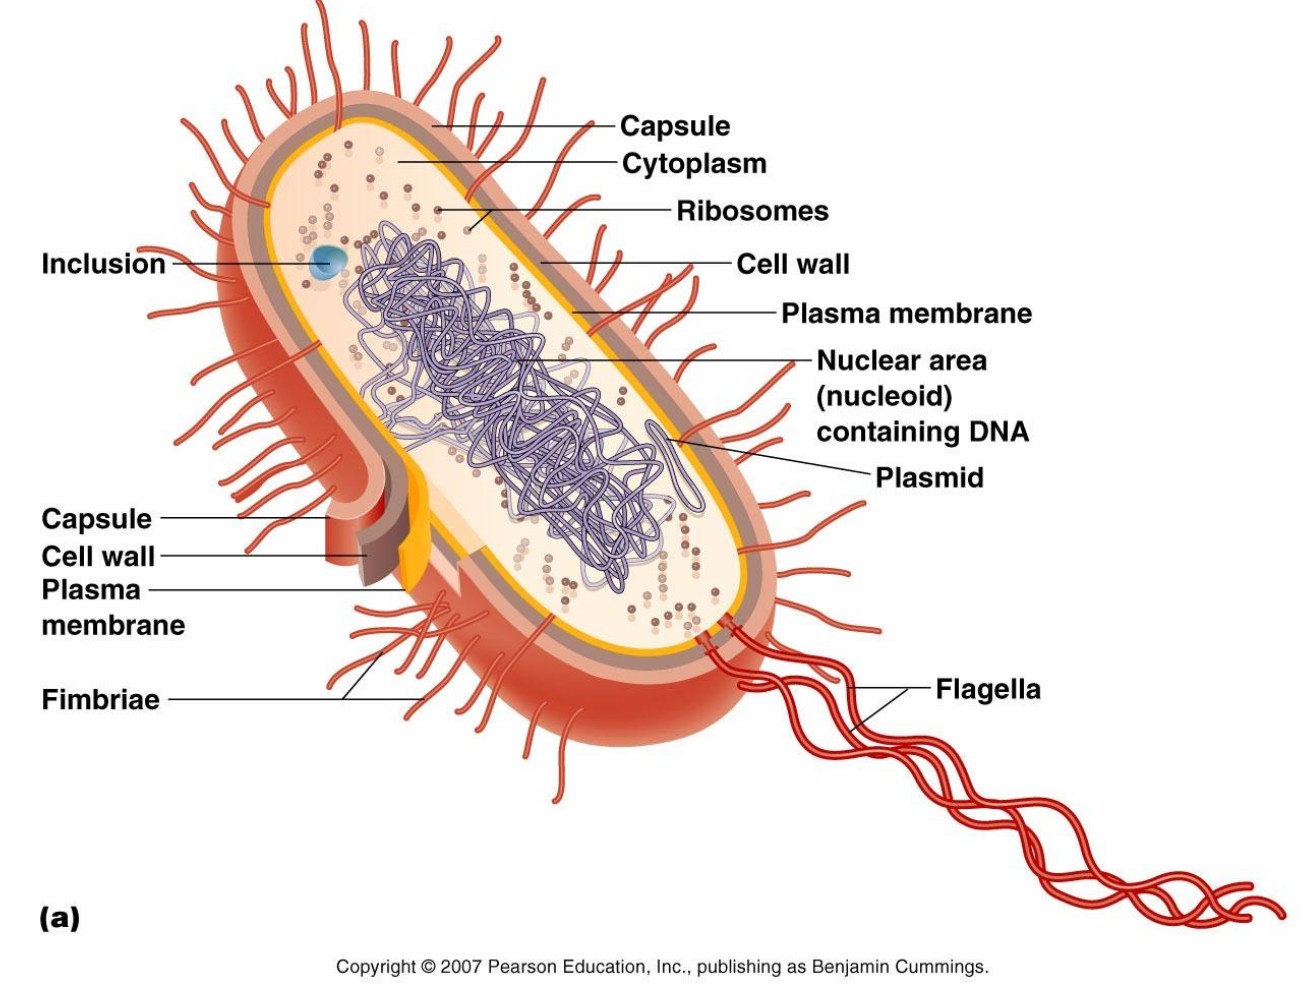
\includegraphics[width=0.7\linewidth]{figures/Staph/bacterialstructure.jpg}
            \caption{Overview of a rod-shaped Gram-positive cell with a capsule. Image property of Pearson Education.}
            \label{figure:capsule}
    \end{figure}

    \begin{figure}[ht]
        \centering
            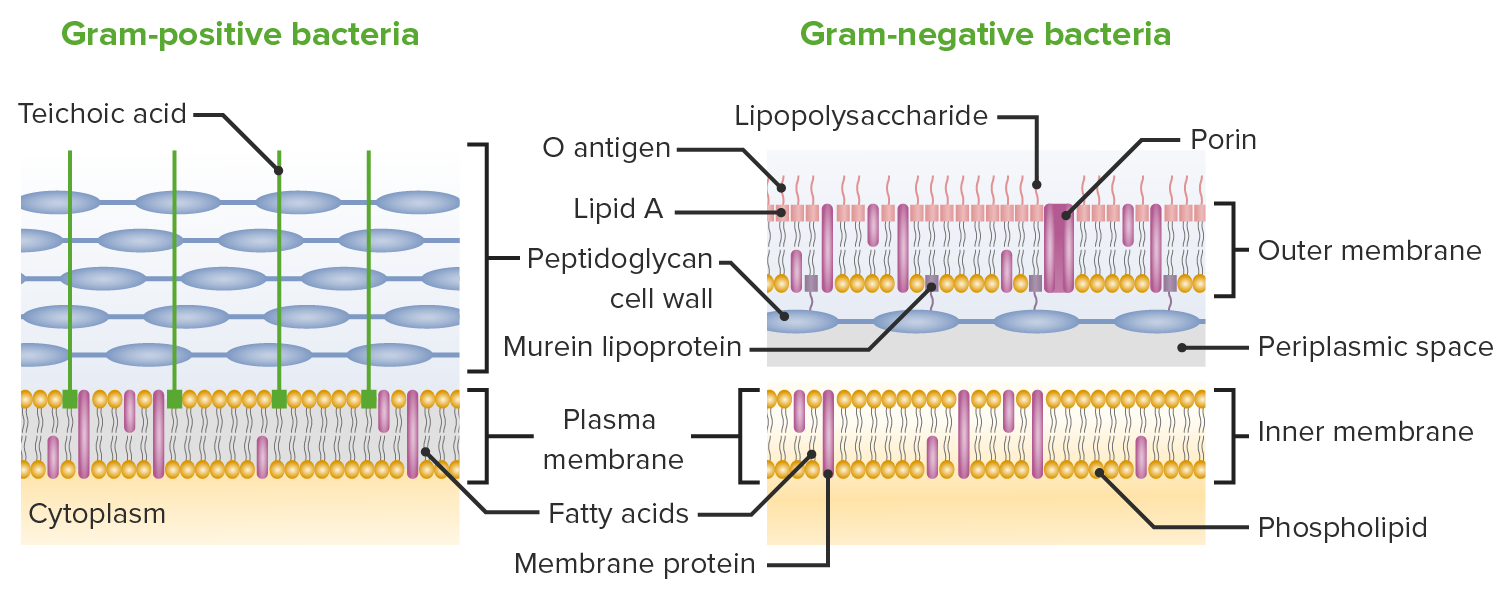
\includegraphics[width=0.7\linewidth]{figures/Staph/Differences-between-gram-positive-and-gram-negative-bacteria-cell.png} 
            \caption{Differences between Gram-positive and Gram-negative cell wall and cell membranes. Reproduced from \url{https://www.lecturio.com/}}
            \label{figure:gram}
    \end{figure}

\subsubsection{Glycocalyx}

Is a gelatinous layer just outside the cell envelope. An irregular gel-like glycocalyx that varies in shape and density is called a slime layer, whereas a distinct more rigid one is called a capsule. In both cases, it serves as a protective function, preventing desiccation, detergents, heat, antibiotics, and phagocytosis. And also in both cases, it contributes to the bacterial structural integrity. 

In addition to protecting the cell from environmental stresses, the glycocalyx particularly the slime layer plays a role in attachment to substrates and host tissue. This is particularly annoying for the host, as the slime layer can help them to stick to tissues or implants and evade the immune system. This is critical for the formation of biofilm, which will be discussed later.

\subsubsection{Outer membrane}
\label{staph:OuterMembrane}

\colorbox{Lavender}{\textcolor{white}{In Gram-negative only.}} The outer membrane contains Porins, which are beta barrel proteins (holes) that open a channel so  specific types of molecules can be transported inside or outside of the cell. Porins also exist in Gram-positive mycobacteria.

It also contains \gls{lps}. These are large molecules that are toxic to humans but are not released from the bacteria towards the host, so they are denominated endotoxin (within-toxin) and are often a synonym of LPS. They are characterized as being very antigenic (polysaccharide O-antigen) and pyrogenic (lipid A) by activating \gls{il1} (fever and inflammation) and \gls{tnfa} (recruiting white blood cells and endothelial activation) Detail about these cytokines will be explained in the inflammation background (chapter  \ref{ch:inflammation}).

\subsubsection{Intermembrane space}

\colorbox{Lavender}{\textcolor{white}{In Gram-negative only.}}. The cell wall is contained within the intermembrane space. So everything that is proper of the cell wall is also in here. Within this space, molecules can accumulate, in particular $\beta$-lactamase, which is very significant in antibiotic resistance.

\subsubsection{Cell wall}

\colorbox{Purple}{\textcolor{white}{In Gram-positive}} bacteria is composed of many peptidoglycan layers, and teichoic acid which is specific to each bacteria species and it allows to bind to fibronectin which will become relevant later on. A peptidoglycan is simply a chain made of peptides and carbohydrates that gives structural support to the cell and gives protection against osmotic damage.

\colorbox{Lavender}{\textcolor{white}{In Gram-negative}} bacteria, it only has a very thin cell wall composed of fewer layers of peptidoglycans.


\subsubsection{Inner membrane}

\colorbox{Purple}{\textcolor{white}{Gram-positive}} bacteria are the only ones that have lipoteichoic acid. It is a regulator of autolytic wall enzymes (prevent the cell from killing itself) and it has specific antigenic properties.

Both \colorbox{Purple}{\textcolor{white}{Gram-positive}} and \colorbox{Lavender}{\textcolor{white}{Gram-negative}} have a phospholipid bilayer, carbohydrates and proteins. In particular, enzymes are responsible for cell wall synthesis and \gls{pbp}. When penicillin binds to PBP, the cell can't make cell walls, and it dies either from collapsing or osmotic damage. Human cells are unaffected by penicillin because eukaryotes cells regulate osmotic damage directly in the cell membrane, and because their structure is supported by their internal cytoskeleton. Bacteria's inner membrane can also protect from osmotic damage, but it relies more on the cell wall for that function.

\subsection{Gram Staining}

The technique consists of three steps:

    \begin{enumerate}
    
        \item Adding crystal violet stain to a bacterial sample. As Gram-positive bacteria have a much thicker peptidoglycan layer they bind to it. Making them more violet-saturated than the Gram-negative. Technically this is all you need, but trying to identify the type by just the violet saturation would render many false positive errors. The next two steps correct this.

        \item Wash out the crystal violet with ethanol, Gram-positives are much harder to wash and the violet color will remain on it while Gram-negatives are decolorized which are difficult to see under the microscope. Thus the next step.

        \item Add a counterstain of Safranin or Fuchsine. Gram-positive will remain violet while Gram-negative will gain a fuchsia color.

    \end{enumerate}

\subsection{Morphology and arrangement}

    \begin{figure}[ht]
        \centering
            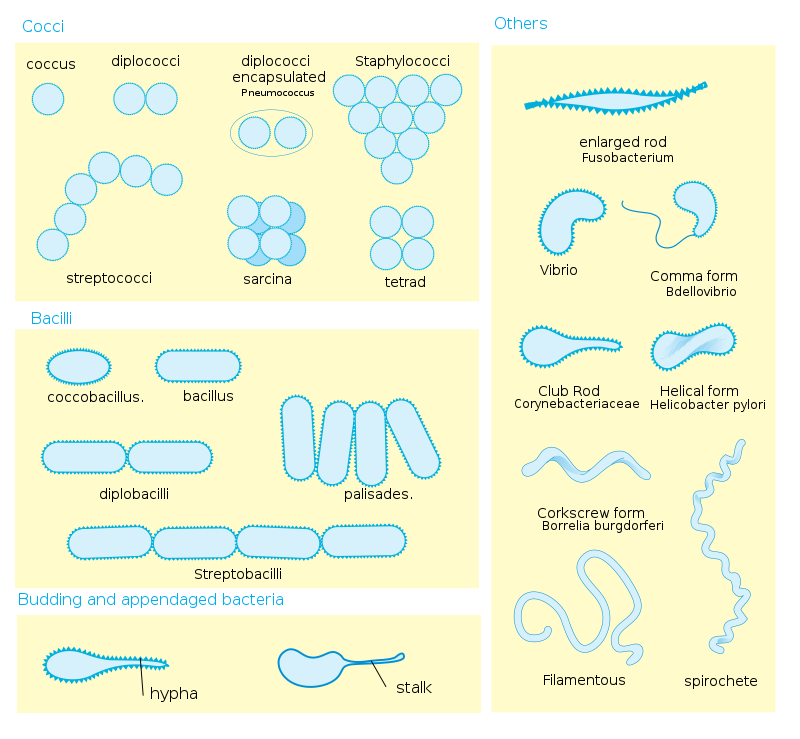
\includegraphics[width=0.7\linewidth]{figures/Staph/Bacterial_morphology_diagram.svg.png} 
        \caption{Different types of bacteria morphologies. Source: Wikimedia.}
        \label{figure:bacteriashapes}
    \end{figure}

Both Gram types can be either cocci (round) or rod-shaped. Rods are also referred to as bacilli, but these are not to be confused with the genus \textit{Bacilli}. Bacteria are italicized in text, as such \textit{Staphylococcus Aureus} is italicized in this thesis. A better example is \textit{Haemophilus influenzae} a bacterium, which shall not be confused with influenza, not italicized, hence a virus. \textit{Staphylococcus} refers to the genus, while \textit{aureus} refers to the species. As the name suggests, \textit{Staphylococcus Aureus} is a cocci bacterium arranged in clusters. Other less common morphologies are included in \ref{figure:bacteriashapes}. 

\subsection{Gram-positive characterization}

\subsubsection{Spore formation}

Rods can be spore-forming or non-spore-forming. Both are sub-categorized into aerobic, and anaerobic. Furthermore, both are divided into Motile and Immotile. They are beyond the scope of this thesis.

Gram-negative bacteria never make spores. However some Gram-positive bacteria can make endospores under some conditions, typically unfavorable environments. This effectively means that they transform from a vegetative state (capable of reproduction) into a spore state, which is a dormant state in which the bacteria are encased and protected by multiple layers of Calcium-Dipicolinic acid. This is the reason why some bacteria are heat resistant, and boiling things, such as your food, can kill some bacteria but not all of them. And why we use autoclaves to sterilize instruments at 121ºC at 15psi for nearly 60 minutes.

\subsubsection{Catalase}

Catalase is an enzyme that catalyzes the conversion of \ch{H2O2} into \ch{H2O} and \ch{O2}. Cocci can be catalase positive forming cocci bundles such as \textit{S. Aureus}, or catalase negative forming cocci rows such as \textit{Streptococci}. A quick test with no microscope, stains, or culture, for bacterial infection is to drop some \ch{H2O2} on it, and if it bubbles (\ch{O2}) it means you have a \textit{Staph} group, and is immune to oxidative burst by neutrophils.

Catalase positive can be divided further using a coagulase test. If the test is positive it means that the sample is a \textit{Staph aureus}. If the test is negative you flood the sample with an antibiotic called novobiocin. If the bacteria die, it means that you have a \textit{Staph epidermis}, but if it is resistant it means that you have \textit{Staph saprophylicus}

Catalase negative are organized in chains, such as the \textit{Streptococcus}, and are classified according to their hemolytic activity. This means they can break down or not red blood cells. Here I will give you some clinically relevant examples.

\begin{itemize}

    \item \textbf{Partial hemolytic ($\alpha$)} Do an optochin resistance test (another antibiotic), if it is sensitive then is \textit{S. Pneumoniae}, if it is resistance you have \gls{vgs}.
    
    \item \textbf{Total hemolitic ($\beta$)} Do another antiobitic resistance test with bacitracin. If it is sensitive you have a \gls{gas} such as \textit{Streptococcus pyogenes}. If it is resistance, you have a \gls{gbs} such as \textit{S. agalactiae}.
    
    \item \textbf{No hemolitic ($\gamma$)} Try to grow it in a \ch{NaCl} solution. If it grows, you have \textit{Enterococci}. If it kills the bacteria, you have \textit{S. Bovis}.
    
\end{itemize}

    \begin{figure}[h!]
        \centering
            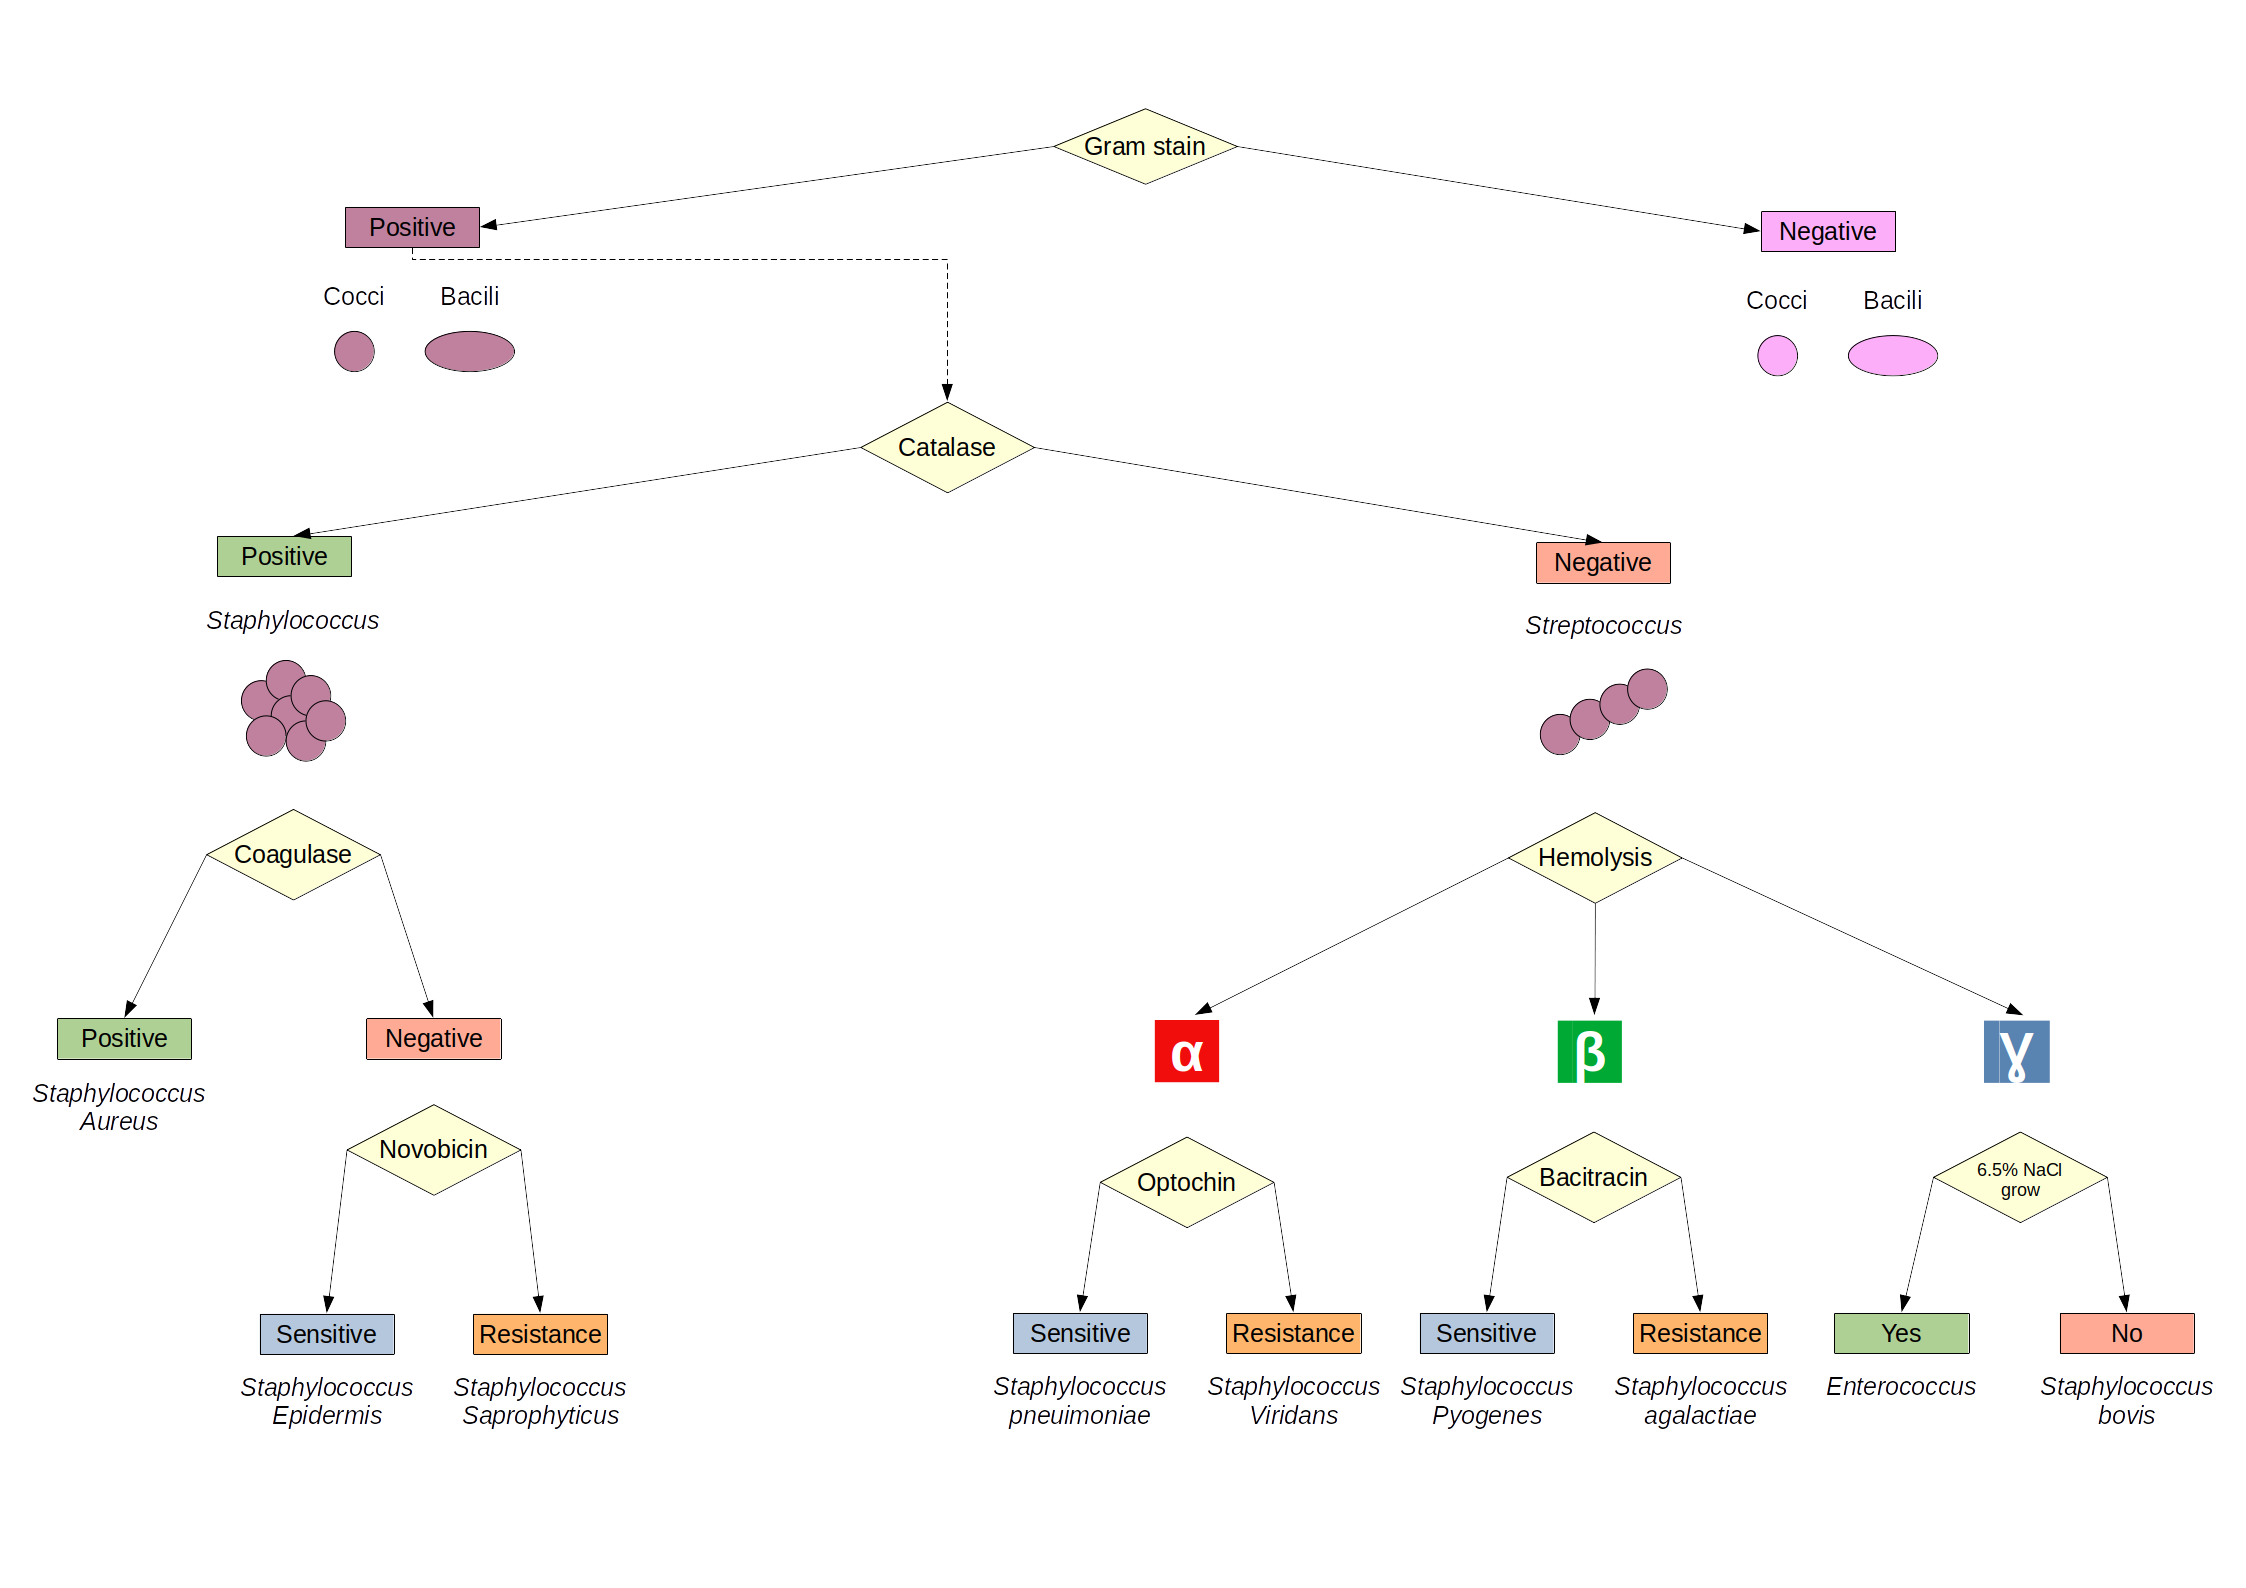
\includegraphics[width=0.9\linewidth]{figures/Staph/Identification.png}
            \caption{Overview of \textit{S. Aureus} identification and other bacteria. Self-made figure.}
            \label{figure:identification}
    \end{figure}

\subsubsection{Fibrin}
\label{staph:Fibrin}

In all cases, all coagulase-positive bacteria lack endospores. "Endo" means with-in, meaning that even though they cannot make their own spores, they can use external tools to make spores. This is the case of Fibrinogen which is found in the human body, and \textit{Staph} uses it to convert it into Fibrin, utilizing coagulase to do so. Effectively, this is employed to hide from the immune system. As a result, coagulase-positive bacteria are highly localized but vary in infection size (folliculitis, abscesses, furuncles, and carbuncles). While coagulase-negative bacteria tend to be widespread (sepsis, cellulitis, necrotizing fasciitis)

Localized bacteria have the advantage that they can be a threat with an incision and drainage as opposed to a widespread infection. The disadvantage is that it exerts much more pressure in the area, especially inside the skull when dealing with brain abscesses.

\section{S. Aureus main characteristics}

\subsection{Bacterial properties}

\textit{S. Aureus} is a prokaryote Gram-positive bacteria capable of growing in both aerobic and anaerobic, and a variety of acidic or based places, although it prefers aerobic and neutral acidic environments such as the skin.

\subsection{Structural components}

\subsubsection{Glycocalix}

The \textit{S. Aureus} can have both a capsule and a slime layer depending on the strain. The \textit{S. Aureus} capsule inhibits phagocytosis as with many other bacteria capsules. Finally, the capsule is prone to contain adhesin proteins which help \textit{S. Aureus} adhere to the epithelium of the mucosa, such as skin, nasopharynx, oropharynx, gastrointestinal tract, and in neonates umbilical stump and peri-anal area. The \textit{S. Aureus} slime layer is prone to forming biofilms. \cite{Parastan2020}

% Lot of sources here: https://www.sciencedirect.com/science/article/abs/pii/S2452014420301539

A biofilm is a community of microorganisms, including bacteria, that stick together on a surface. The biofilm is composed of many layers of cells and \gls{eps}. The EPS is a sticky layer mostly formed by polysaccharides secreted by the bacteria that helps them stick to anything, particularly room surfaces, human tissues, or medical equipment. The EPS also provides a barrier against harmful agents and promotes nutrient exchange and communication between adjacent cells.

    \begin{figure}[h!]
        \centering
            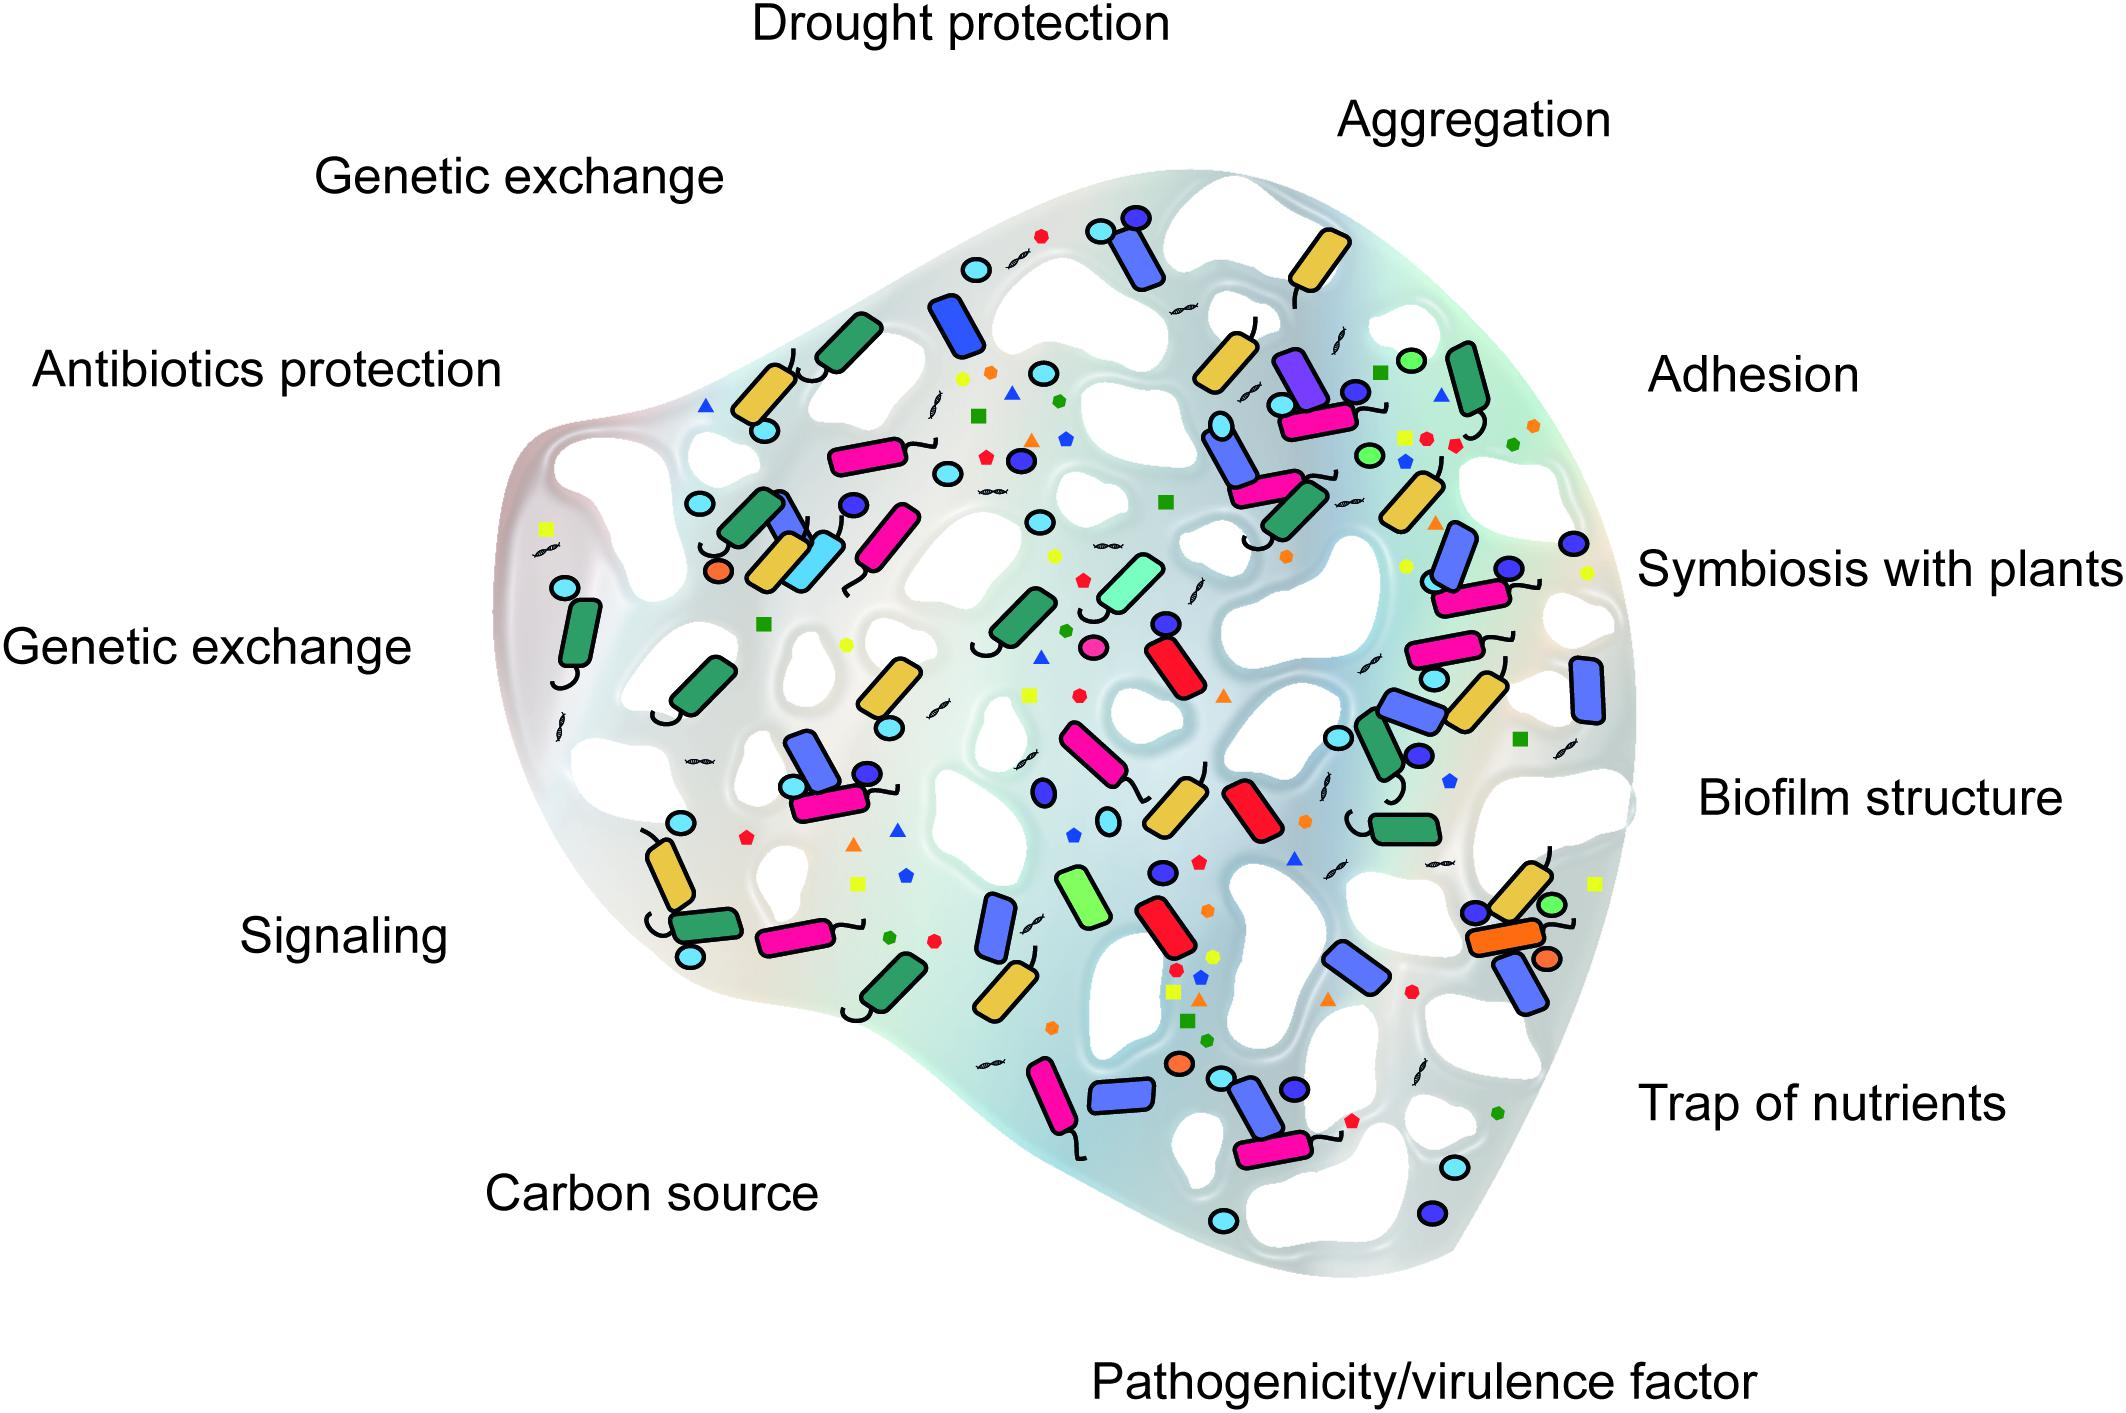
\includegraphics[width=0.7\linewidth]{figures/Staph/fmicb-09-01636-g001.jpg } 
        \caption{Conceptual framework of the functions of microbial extracellular polymeric substances (EPS) in soil. Reproduced from \url{https://doi.org/10.3389/fmicb.2018.01636}}
        \label{figure:EPS}
    \end{figure}

Biofilms are often associated with infections. They are very difficult to detect or treat. The immune system is often unable to break throw the protective exopolysaccharides layer. Antibiotics stay in the blood for a short time and are also unable to penetrate the biofilm, and in the meantime, bacteria hide inside. Biofilms are also the ideal breeding ground for new strains given their protected environment.

\subsubsection{Cell Wall}

The peptidoglycan in the cell wall in the \textit{S. Aureus} is not special. But it provides surface adhesion proteins that have a very special function. They adhere to the peptidoglycan cell wall (bacteria) and at the same time to fibronectin, fibrinogen, collagen, or elastin (human tissue). Technically, it helps the immune system recognize the bacteria which is why are called \gls{mscramm}. But in the \textit{S. Aureus} case, it does the complete opposite:

\begin{itemize}

    \label{stephCellWallSPA}
    \item \textbf{\gls{spa}} arrest antibodies by binding to the constant part of the \gls{igg}, preventing antibody-mediated immune clearance of the \textit{S. Aureus}. Furthermore, this forms an antigen-antibody complex, which activates the classical complement pathway of the complement immune system, wasting it, and leading to hypocomplementemia.

    \item \textbf{Other surface proteins} \textit{S. Aureus} also have \gls{sasc} \cite{Foster2013} \gls{sasg} \cite{Cheng2009} and \gls{sasx} \cite{Josefsson2001}. All of them promote adhesion to desquamated epithelial cells and contribute to biofilm formation.
    
    \item \gls{fnbpa} connect the bacteria with fibronectin and fibrinogen (human parts), which is critical for \textit{S. aureus} virulence. It enables the bacterium to colonize and infect host tissues. In addition, FnBPA contributes to the formation of biofilms. Several small-molecule inhibitors and monoclonal antibodies against FnBPA have been developed and tested in pre-clinical studies approaches for the treatment and prevention of \textit{S. Aureus} infections associated with medical implants.

\end{itemize}

\subsection{Enzymes}

\subsubsection{Coagulase}
\label{stahp:coagulase}

In vertebrates, thrombin converts fibrinogen into fibrin, which later on will form a blood clot aimed to stop hemorrhages. Fibrin also reduces thrombin activity and promotes angiogenesis. All of these are used by \textit{S. Aureus} to its advantage, defining its coagulase abilities.

\gls{clfa} and \gls{clfb} transform fibrinogen into fibrin. They both bind to fibrinogen and promote clotting, forming a shell around the \textit{S. Aureus}, which is the way \textit{S. Aureus}, a coagulase-positive bacterium that lacks endospores as any other, can make something similar to endospores which helps it hide from the immune system on highly localized surfaces. This also serves as an adhesion protein that binds the peptidoglycan cell wall to other surfaces and tissues.

Another feature of \textit{S. Aureus} is its ability to secrete staphylocoagulase and \gls{vwbp}, binding to human thrombin and forming staphylothrombin. Which further promotes fibrinogen to fibrin conversion, forming even more clots.

Interactions of \textit{S. Aureus} and platelets play an important role in the pathogenesis of intravascular infections such as \gls{ie}. A typical feature of \textit{S. aureus} is the ability to generate thrombin activity through the secretion of two prothrombin-activating molecules, staphylocoagulase and \gls{vwbp}, which bind to human prothrombin to form the enzymatically active staphylothrombin complex. The role of staphylothrombin in the interaction between \textit{S. aureus} and platelets have not yet been studied. \cite{Vanassche2012}

\subsubsection{Hyaluronidase}

Hyaluronidases are a family of enzymes that catalyze the degradation of hyaluronic acid. \gls{staph} produce hyaluronidase to obtain carbon from hyaluronan which is abundant in epithelial tissue. Is speculated that \gls{staph} uses Hyaluronidases to destroy the polysaccharide in cells, making it easier to infiltrate in the host.

\subsubsection{Staphylococcal Fibrinolysin}

It is a powerful fibrinolytic enzyme that helps the bacterium to dissolve blood clots in order to spread throughout the host. Staphylokinase plays a key role in the virulence of \textit{S. Aureus} by allowing the bacterium to invade and spread through tissues, in particular the formation of abscesses. It also breaks \gls{igg} and \gls{c3b}, inhibiting phagocytosis, and contributing to hypocomplementemia.

\subsubsection{Lipase}

\textit{S. Aureus} produces lipase to digest lipids into fatty acids and glycerol, which later are turned into ATP. Lipids are also a major component of skin (and other tissues), which helps to colonize human skin more effectively. Lipids also happen to be hydrophobics. As such, when added to the biofilm, lipids help to protect the bacteria against antimicrobial agents.

\subsubsection{Nuclease}

\label{staphNuclease}

A nuclease enzyme is used to break down DNA components and is a common beneficial enzyme required for the central dogma of molecular biology. In the hands of \textit{S. Aureus} however, it breaks down the host DNA into its individual components which the bacterium uses as a source for ATP and other common cellular requirements. This is especially important when the bacteria infiltrate parts of the body where resources are scarce.

Neutrophils can commit suicide as a last method of attacking pathogens by projecting their DNA and using it as a net to catch the invader. This is known as \gls{nets}. Nuclase can break down this trap, allowing it to continue infecting the host. Furthermore, this can also damage healthy cells' DNA prompting apoptosis. All combine to contribute to tissue damage and inflammation.

\subsubsection{Collagen adhesin}

\gls{cna} is a protein that facilitate adhesion to collagen-rich tissue \cite{Patti1994} \cite{MURUGAN2010}. Especially important in the biofilm formation for ocular keratitis and septic arthritis.

\subsubsection{Iron-regulated surface protein}

\gls{isda} and \gls{isdb} facilitate the adhesion to desquamated epithelial cells and promote iron acquisition, typically obtained from the effect of hemolysin. It helps with nasal colonization. \cite{Foster2013} \cite{Cheng2009}

\subsection{Toxins}

\subsubsection{Hemolysin}

This leads to the destruction of the red blood membrane, releasing their hemoglobin, which is used as a source of iron, which is essential for bacterial growth. Secondarily, it can aid immunoevasion because the destruction of red blood cells will lead to inflammation. This means that the immune system will divert resources to soften the inflammation instead of fighting the bacteria. Inflammation can further increase blood permeability allowing the \gls{staph} to transverse blood vessels invading different tissues.

\subsubsection{Exfoliative Toxins}

In between skin cells, keratinocytes, there is a protein called desmoglein-1 which attaches them together packing the skin tight. Exfoliative toxins will damage this connection so they can't stay linked together, leading to patches of the skin falling off. This is the reason why Nikolski's sign symptom manifests in some \textit{S. Aureus} related diseases.

\subsubsection{Enterotoxins}

This targets the enterocytes in the \gls{git}, creating pores on them leading to the destruction of the cell membrane. The sodium inside those cells and other electrolytes leak out, making it more difficult for the rest of the GIT to absorb nutrients, which causes diarrhea. This also damages the epithelium cells of the GIT causing gastroenteritis.

\subsubsection{Panton–Valentine leukocidin (PVL)}
\label{staphPVL}

\gls{pvl} creates pores in leukocytes which lead to ions imbalance making the leukocytes die. This leads to inflammation, particularly in the lungs.

\subsubsection{TSST-1}
\label{staphTSST1}

\gls{tsst1} is a toxin which can be released by \textit{S. Aureus}. This toxin acts as a superantigen. Antigen Presenting Cells have \gls{mhc2} that interact with other cells like T-cells via their CD4 protein. TSST-1 acts as a bridge between the two a hyperstimulates their response leading to a cytokine storm of \gls{il1}, \gls{il2}, \gls{tnfa}, and \gls{ifng}. All of these proteins lead to an inflammatory reaction that acts on the skin creating a rash. They also increase capillary permeability causing vasodilation of the blood vessels leading to both hypotension and hypovolemic shock. Finally, they also increase prostaglandins in the hypothalamus, which leads to fever.

\section{Staph diseases}

\gls{staph} is usually harmless and will just colonize the skin and nasopharyngeal track of the host. However, is also an opportunistic bacterium that easily attaches to many tissues and can develop much more serious complications there.

\subsection{What causes the disease?}

\begin{itemize}

    \item \textbf{Bacteria.} This is when a direct bacterial invasion. To diagnose it you need to look for \gls{igg} related to the bacteria or to perform bacterial cultures. When there are too many, it leads to bacteremia. Generally, if you want to treat it, you do it with antibiotics.
    
    \item \textbf{Toxins.} This is when the bacteria produce toxins that affect the host and produce symptoms. To diagnose it you need to look for \gls{igg} related to the toxin, not the bacteria. When there are too many toxins, it leads to toxemia. They do not respond at all to antibiotics, and samples will show no growth in bacterial agar plates.

\end{itemize}

First, we are going to list the diseases caused by the bacteria, and then, the diseases caused by the toxins.

\subsection{Skin lesions and infections}

They are highly localized due to the coagulase factors. The common ones are superficial abscesses and folliculitis (hair infection). If this becomes severe and deep, they will turn into furuncles (multiple and deeper folliculitis). If it becomes worse, they will turn into carbuncles.

Carbuncle is a deeper folliculitis with multiple sinus tracks, usually on the back and neck. If it goes deeper it passes the fat layer of the skin and reaches, muscles, bones, or blood vessels. Reaching the blood vessels means reaching the blood, which goes everywhere, thus spreading the bacteria in multiple organ tissues. It can also generate septic embolisms in which pus is dislodged from the original site transverse the blood and might land in an organ. Septic embolisms can also be generated in the newly infected organs reaching other random organs via blood vessels.

\textit{S. Aureus} is the most common pathogen associated with wound infections and the most isolated bacteria from chronic wound infections \cite{Bhattacharya2015} such as diabetic foot ulcers. Wound infections are also a common source of septic embolism, which might be caused due trauma (dirty injury), or surgical equipment, which might not be completely clean due to the biofilm properties of \textit{S. Aureus} discussed before. Or even not clean at all such as dirty needles reutilization in drug users.

Cellulitis is also a common complication of \textit{S. Aureus}, however, due to the coagulase mechanisms it tends to stay focalized rather than spread, so is more likely that cellulitis is caused by strep bacteria. 

Depending on the severity, abscesses are generally treated with incision and drainage. If it is a severe case, systemic antibiotics. If it is so severe that it reaches the bloodstream then intravenous antibiotics.

\subsection{Catheter associated infections}

When surgical equipment, prosthetics, needles, or catheters are inserted into a patient, they need to transverse the skin layer which is rich in \textit{S. Aureus}. Even if the equipment is completely clean, this may lead to \textit{S. Aureus} being attached to the equipment, forming a biofilm around it, and staying in the bloodstream until the device is removed. At the same time, the biofilm can release bacteria leading to bacteremia in the blood and spreading everywhere else.

\subsection{Pyomyositis}

Pyomyositis is a bacterial infection of the skeletal muscles which, typically results in an abscess. In the case of \textit{S. Aureus}, secondary pyomyositis which is localized is more frequent. Internal imaging such as CT scans or MRI is required to assess the lesion extension.

\clearpage

\subsection{Endocarditis}

Types of bacterial endocarditis are:

\begin{itemize}

    \item \textbf{Acute.} High-virulence organisms are invading and destroying an intact and healthy heart valve. The \textit{S. Aureus} acts in this group.
    
    \item \textbf{Subacute.} Weak bacteria are attacking a weak valve. Examples of these are the \gls{hacek}.
    
\end{itemize}

It should present with a fever, due to the \textit{S. Aureus} \gls{mscramm} and cloths, and with a new murmur due to the patient having a previously healthy valve. Since the bacteria is already in the blood, it can be diagnosed using a blood culture.

\subsection{Lung abscesses}

Similar to endocarditis, \textit{S. Aureus} goes into the blood and lands in the lungs. Usually causing an excessive amount of liquid (pus) to be allocated in the pleural space in the lung (pleural empyema). It causes productive cough, hemoptysis, or even necrotizing pneumonia. Besides the blood culture, it can also be diagnosed by sputum culture.

\subsection{Brain abscesses}

Similar to endocarditis and lung abscesses, \textit{S. Aureus} goes into the blood and lands in the brain, causing meningitis or brain abscesses. Previously we discussed that \textit{S. Aureus} is heavily localized, it doesn't spread but in exchange can increase pressure in the infected area. This is not a problem in places where it has space to grow, such as the skin. But the skull is 100\% pack with no room for anything else which leads to the increase of \gls{icp}.

This leads to any sort of focal neurological symptoms, as well as classical ICP such as morning frontal headache, projectile vomiting, and blurry vision. When doing a lumbar puncture, it might present an increase exit pressure.

\subsection{Osteomyelitis and septic arthritis}

Once again, \textit{S. Aureus} goes into the blood, which goes into the bone, bone marrow, and joints. However, it can also be caused by direct trauma from something dirty that penetrates the skin and reaches the bone, such as a knife or a bullet.

    \begin{figure}[h]
        \centering
            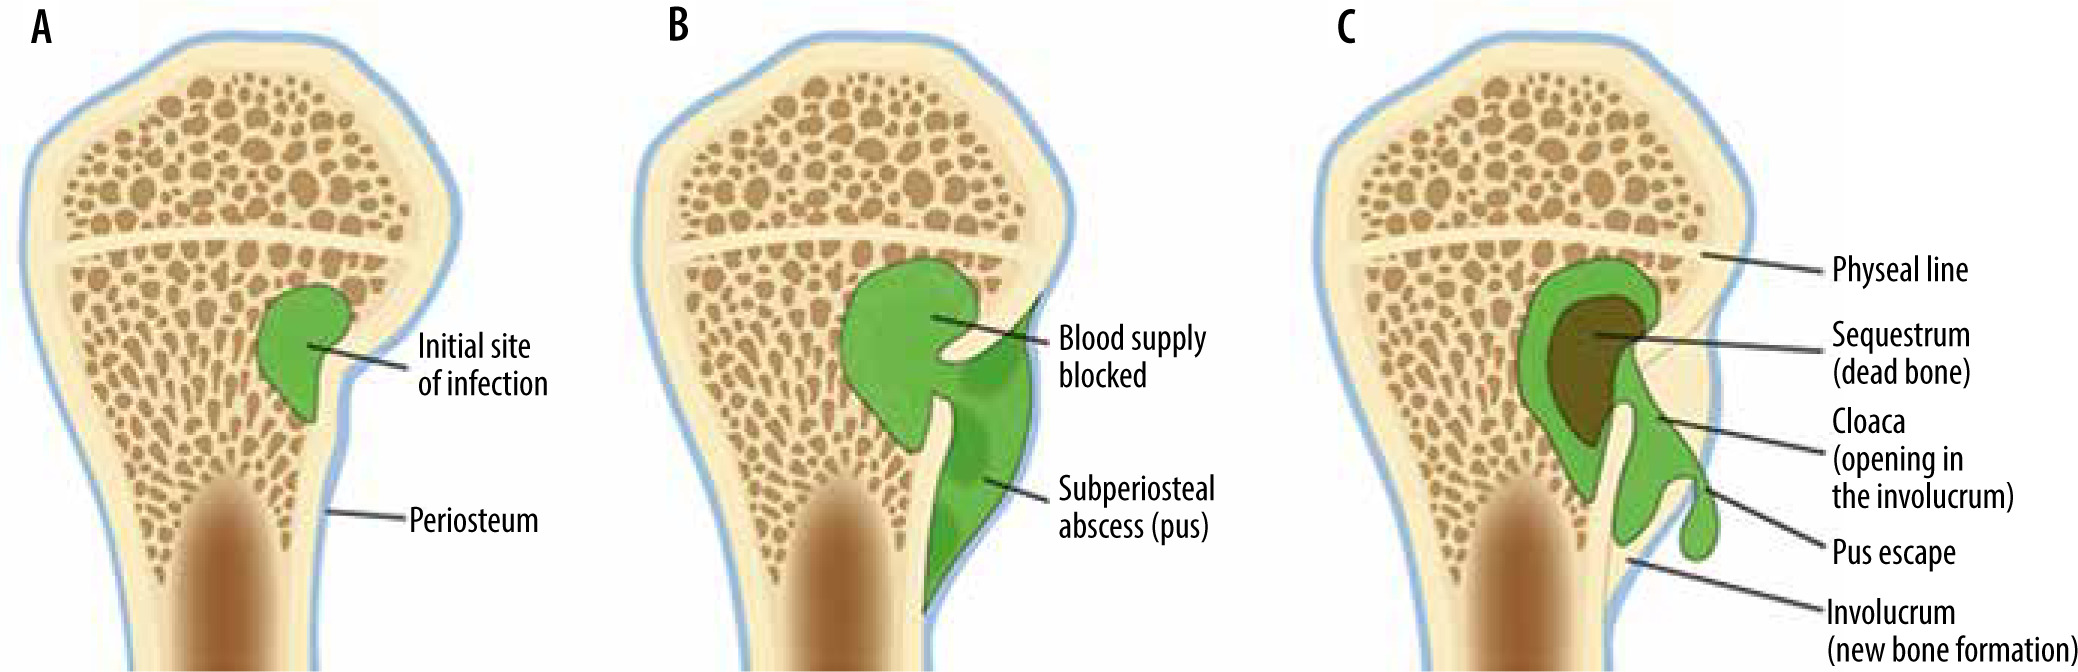
\includegraphics[width=0.7\linewidth]{figures/Staph/PJR-87-46472-g022.jpg} 
        \caption{An artist’s drawing of osteomyelitis progression, subacute to chronic. A) Initial site of osteomyelitis involving the medial aspect of the long bone metaphysis/intraosseous abscess (green). B) The abscess extends through the cortex into the subperiosteal space forming a subperiosteal abscess (shades of green). C) Chronic osteomyelitis with a detached central necrotic bone fragment/sequestrum (brown) within the intraosseous abscess (green) with peripheral new bone formation/involucrum and a cortical and periosteal opening in the involucrum/cloaca allowing the pus to escape. Reproduced from \url{ https://doi.org/10.5114/pjr.2022.113825}}
        \label{figure:osteomyelitis}
    \end{figure}

Is likely to be caused by the metaphysis of the bone due to the stagnated blood circulation in that area, and due to the cartilage blocking the path to the epiphysis. It might lead to septic arthritis (inflammation of the joints), fracture, growth disruption, and vertebral osteomyelitis which can destroy the vertebral cord and develop neurological symptoms. Infections in bones are difficult to treat, which might lead to chronic osteomyelitis, developing into further complications such as sclerosis or the need for amputations.


\subsection{Staphylococcal Scalded Skin Syndrome}

\gls{ssss} is a skin infection. This infection mainly affects patients with weak immune systems, such as babies, children, old individuals, or HIV patients. SSSS is characterized by blistering of the skin similar to a sunburn-like rash, and the skin may feel like it is scalded. It leads to peeling and shedding of the top layer of skin just with mild pressure to the touch (Nikolsky's sign).

It doesn't present any inflammation, no cytolysis, no leukocytosis, and no bacterial growth in cultures because this is not caused by the \textit{S. Aureus}, it is caused by the exfoliative toxins A and B. It heals on its own in about 7 to 10 days and requires only palliative care. However, immunocompromised patients have a mortality rate of 60\%.

\subsection{Ocular infections}

Keratitis is a condition in which the cornea becomes inflamed. This can be caused by introducing \textit{S. Aureus} in the eye, via injury, or dirty contact lenses. Similarly, conjunctivitis can occur. If the infection penetrates deeper into the eye it can turn into endophthalmitis. \cite{MURUGAN2010}

\subsection{Bullous Impetigo}

Is a yellowish crust sore on the skin, normally in areas with skin folds. Is a localized form of \gls{ssss} and is only caused by a specific strain. Is treated with systemic antibiotics such as oral cephalexin. Nonbullous impetigo can be caused by staph or strep bacteria and it can be less severe. In such cases, topical antibiotics can be used.

\subsection{Food poisoning}

If you ever went to a dirty restaurant and ended up vomiting or having diarrhea, is likely that an enterotoxin was the cause. \textit{S. Aureus} have \gls{sea} and \gls{seb}. They are heat resistant and remain even after cooking the food, meaning that you killed the bacteria, but not the toxin. Is likely that the \textit{S. Aureus} ended up in the food due to the chef touching his nose with his fingers, regardless of whether he wore sanitary gloves or not. If food is left uncooked at room temperature it will give \textit{S. Aureus} a better chance to reproduce and create even more toxins. \textit{S. Aureus} also survives in salt.

SEA causes gastroenteritis, it presents no fever and it leads to nausea, vomiting, and watery diarrhea. It usually appears after 5 hours of incubation and resolves itself in less than 24 hours. Treatment includes normal saline for severe cases of dehydration and \gls{nsaids} for severe pain.

SEB cause gastroenteritis and enterocolitis. SEB is a superantigen, which causes the immune system to release a large number of cytokines, which means fever and inflammation. 

\subsection{Toxic Shock Syndrome}

The mechanism described for \gls{tsst1} in section \ref{staphTSST1}, leads to Toxic Shock Syndrome. It usually happens when external objects are left inside the body for too long and do not have an antibiotic coating, such as surgical cures or tampons.

\subsection{Necrotizing Pneumonia}

The mechanism described for \gls{pvl} in section \ref{staphPVL} might kill lung cells which leads to this disease.


\subsection{Antibiotics resistance strains}

\gls{mssa} is vulnerable to various common Methicillin-family antibiotics such as oxacillin, cloxacillin, dicloxacillin, and nafcillin. As the name suggests, also vulnerable to methicillin, which back in time was great because it was a $\beta$-lactamase resistant penicillin. On the bad side, turns out that methicillin also kills the kidneys via interstitial nephritis, which is why methicillin is not used anymore and similar alternatives of the same antibiotics family are used.

As time passed a new strain developed resistance to everything, called \gls{mrsa}. This is due to the bacterium's brand new mecA gene that encodes and produces a \gls{pbp} named PBP2a. This is present in the bacteria cell membrane instead of the original PBP, however, because the structure is different, penicillin (or Methicillin-like antibiotics) can't bind to it anymore. The solution was simple, use Vancomycin to kill the MRSA, especially the hospital-acquired MRSA.

As time passed a new strain came, \gls{vrsa}, which has a brand new van-A gene that alters the peptidoglycan cell wall structure, so the Vancomycin can't prevent cell wall formation anymore. VRSA is treated with Linezolid, daptomycin, telavancin, or ceftaroline. Linezolid is really good but really expensive.

In 2001 there was the first reported case of \gls{lzrsa} \cite{Tsiodras2001}. Then 2006 in China \cite{Jones2007}, 2008 in the US \cite{Mendes2008}, 2006 to 2008 in Japan \cite{IkedaDantsuji2011}, 2008 to 2009 in Spain \cite{Seral2011}, and 2010 in Italy \cite{Mendes2010}. As the reader might have imagined, we already have LZR \textit{Staphylococcus Aureus}. The incidence of LZR staphylococci is still low, but this may change any day due to antibiotic abuse. Limiting hospital stances and antibiotic abuse is critical to limit new antibiotic-resistant strains. LZRSA is currently treated with daptomycin and tedizolid, however, these two antibiotics have severe adverse effects.

\section{Identification}

\subsection{Microscopy}

Direct observation of \textit{S. Aureus} is possible from skin or pus samples. After applying Gram-stain, you should be able to see purple spherical bacteria in cluster form. In bacteremia cases is also possible to observe it blood after culture of the blood sample. Microscopy is a very fast and cheap method as long as the culture is not needed.

\subsection{Culture}
\label{staph:culture}

\textit{S. Aureus} can grow in selective or non-selective media. In selective media, it can trigger false positive results due to the culture being contaminated with other fermentation bacteria, in which case you can add 7.5\% \ch{NaCl} which will kill many other microbes leaving \textit{S. Aureus} alone. It can grow in aerobic or anaerobic and at room temperature. It would grow in around 24 hours and form yellow-orange-ish colonies. It may also present with a green area due to the \textit{S. Aureus} hemolysins partially break down hemoglobin or present a lack of red due complete breakdown of the hemoglobin. Very cheap, and relatively fast.

The culture supernatant can also be tested for the presence of toxins using a biological assay such as a mouse bioassay or a cell cytotoxicity assay.

\subsection{Nucleic Acid Amplification Test}

\gls{naat} consists of amplifying the genetic material of the bacteria, reading the sequencing, and comparing with a database to match \textit{S. Aureus} or any other pathogen. Results are done in about 3 hours but are more expensive.

\gls{pcr} is a commonly known NAAT. This test is highly sensitive and specific and can also be used to detect very low levels of toxins.

\subsection{Biochemical tests}

\subsubsection{Coagulase test}

There are two main methods, slide agglutination test and  tube agglutination test. In both, you get some plasma from the patient or an animal and add the bacteria. If it clumps, it means the bacteria have coagulase enzymes, such as \textit{S. Aureus}. The first method gives you immediate results, while the second one needs to be placed overnight.

    \begin{figure}[h]
        \centering
            \includegraphics[width=0.7\linewidth]{figures/Staph/coagulase_positive_negative_slide.png} 
        \caption{The slide agglutination coagulase test is coagulase positive when clots (clumps) occur with a clear solution in the background (left). The slide coagulase test is coagulase negative when there is a smooth mixture with a milky background (right). Reproduced from \url{ https://bio.libretexts.org/Bookshelves/Microbiology/Microbiology\_Laboratory\_Manual\_(Hartline)/01\%3A\_Labs/1.24\%3A\_Coagulase_Test}}
        \label{figure:coagualaseSlide}
    \end{figure}


    \begin{figure}[h]
        \centering
            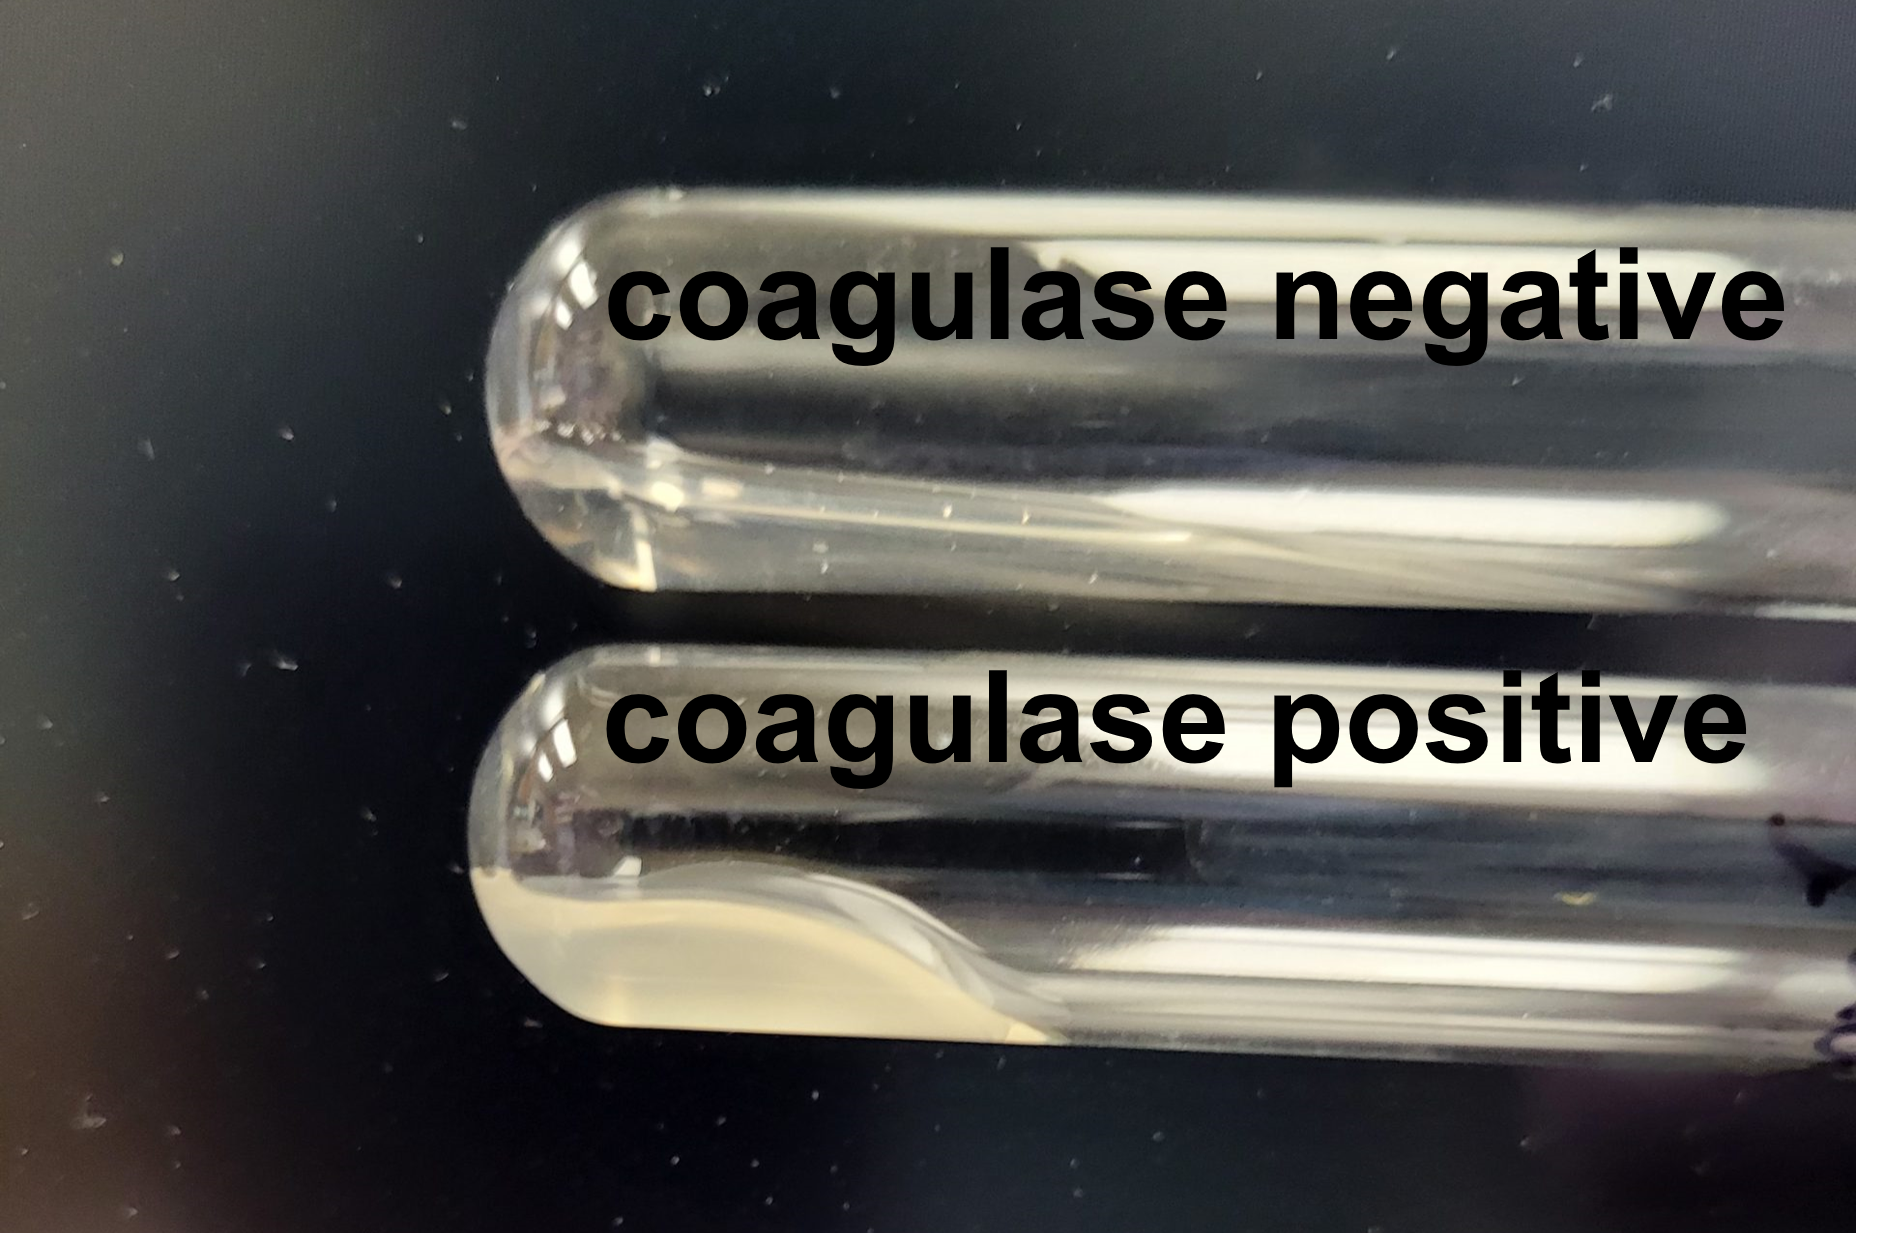
\includegraphics[width=0.7\linewidth]{figures/Staph/coagulase positive negative tube.png} 
        \caption{The tube agglutination coagulase test. When the test tube is tilted, if the fluid is not clumped and does not contain clumps (clotting), the result is coagulase negative (top). When the test tube is tilted, the fluid either exhibits a clump or contains clumps in it (clotting), the result is coagulase positive (bottom). Reproduced from \url{ https://bio.libretexts.org/Bookshelves/Microbiology/Microbiology\_Laboratory\_Manual\_(Hartline)/01\%3A\_Labs/1.24\%3A\_Coagulase_Test}}
        \label{figure:coagualaseTube}
    \end{figure}


Coagulase tests are cheap and quick, but prone to give false positives with other Staphylococcus bacteria such as a novel species the \textit{Staphylococcus Argenteus} \cite{staphArgentusCH}, and false negatives with MRSA strains. There are multiple protocols to add to the test to avoid such misidentifications. \cite{LibreTextStaphID}


\subsubsection{Protein A test}
\label{staph:SPAtest}

The Protein A (section \ref{stephCellWallSPA}) test works by adding a sample from the patient to a plate, usually containing strips coated with antibodies specific to Protein A. If the sample contains \textit{S. aureus}, the Protein A on its surface will bind to the antibodies on the strip, forming a visible line.

\subsubsection{Nuclease test}

\textit{S. Aureus} produce nuclease enzymes (section \ref{staphNuclease}). This test works similarly to the Protein A test. A sample from the patient is added to a plate containing DNA as substrate. After the incubation time period, if the sample contains \textit{S. Aureus} it will break down the DNA leaving empty patches around the bacterial colony.

\subsection{Antibody detection}

An antibody detection test detects the presence of specific antibodies in a person's blood. If the antibodies exist, usually means that a person has developed immunity to the infectious agent.

In the case of \textit{S. Aureus}, it tests for antibodies against the teichoic acids of the bacteria cell wall. If antibodies specific to \textit{S. Aureus} are present in the patient's blood or serum, they will bind to the \textit{S. Aureus} proteins on the plate.

Both Enzyme-linked immunosorbent assay (ELISA) and Immunodiffusion and Western blot can be used to detect specific toxins rather than bacteria.

Generally speaking, antibody detection tests are comparatively quick like NAATs, and much more cheaper. However, antibodies are required to exist in the patient's blood before the test.

\subsection{Mass spectrometry}

Mass spectrometry can't be used to identify the bacteria, but instead can be used to toxins in patient samples by detecting their unique molecular signatures.

\section{Vaccines}

Several vaccines against \textit{S. Aureus} have been developed since 1999 \cite{Parastan2020}, however, due to the bacteria's inmmunoevasive properties, this task has been proven challenging. Furthermore, the safety of these vaccines is still being studied \cite{Xu2017}. Nevertheless, the Staphylococcus aureus 4-Antigen Vaccine vaccine has shown immune Responses up to 36 months \cite{Creech2019}.









% Introduction to Immunology and Inflammation (not ready for review)
%*****************************************
\chapter{Inflammation}
\label{ch:inflammation}
%*****************************************

%*****************************************
\section{Introduction}
%*****************************************

Inflammation has been a well-known condition to mankind since the first time a caveman kicked a rock too hard, and everyone reading this text has experience inflammation in their life. Text from ancient Egyptians used frankincense and myrrh to reduce pain and swelling \cite{Kadioglu2016}. Hippocrates was the first to describe using the word οἴδημα ( /oídēma/, edema) and identify it as an important component of the healing process \cite{Touwaide1999}. In the modern era, the discovery of anti-inflammatory drugs like aspirin and corticosteroids in the 20th century revolutionized the treatment of inflammatory conditions. \cite{Granger2010}

% (maybe add here a paragraph about what are the modern drug targets and genetics and so on)

Inflammation has 4 main characteristics: heat, pain, redness, and swelling. The combination of these may lead to a 5th one which is loss of function in the affected area. The nature of each of these conditions will be revealed throughout this chapter. Inflammation is a natural process that the body uses to fight infections and eliminate the cause of inflammation, clear out the area of elements that shouldn't be there, and repair the tissue if damaged. Similar to fever, it has a bad name with the general population even for mild cases despite being a beneficial and necessary process for recovery. People tend to self-medicate in excess with antipyretics and anti-inflammatories which is counterproductive for both healing processes \cite{Serhan2014}. This process of acute inflammation is inherent to the natural healing process of an organism and overall, the natural pathways of inflammation do not pose a risk to the organism's life, and it is counterproductive to interfere with it, as such interference may ultimately impair the healing process in the long run. On the other hand, autoimmune reactions and chronic inflammations are the undesirable form of inflammation that may lead to lasting damage; often in the form of scar tissue.

At the end of this chapter (section \ref{ref:onlinkPanel}) I discuss the 92 different inflammatory biomarkers upon which the social influence in the inflammation article is founded. However, comprehension of these biomarkers is a complex subject and requires an elaborate introduction to the intricacies of the inflammatory processes. Half of the Inflammation chapter aims to aid the understanding the background of how these 92 biomarkers work. It also serves as a base to further understand the immunoevasion properties of \textit{S. Aureus}, and homeostatic properties of vitamin D. Anyone familiar with immunology should be able to skip directly to section \ref{in:cycle}.

%*****************************************
\section{Immunology basic concepts}
%*****************************************

This section serves as an introduction of basic and easy concepts related to immunity.

\subsection{Reactive Oxygen Species}

\gls{ros} are a natural by-product of cellular metabolism and immune system responses which the influence of heavy metals, tobacco, radiation, or microplastics can overproduce. Excess amounts of ROS damage DNA, lipids, and proteins. This is bad for cells, but good if those cells are bacteria or viruses that we want to destroy.

\subsection{Extracellular matrix}

The extracellular matrix is the material that fills the spaces between cells in tissues and provides the structural support that allows tissues to maintain their shape and function properly. During inflammation, fibroblasts play an important role in the repair and remodeling of damaged tissues. They are activated by cytokines and growth factors that are released by immune cells. As a results they fill the extracellular matrix with collagen, elastin, and fibronectin, which translate into tissue healing.

\subsection{Antigens}

\gls{ag} can be proteins, peptides, polysaccharides, lipids, or nucleic acids. Antigens can be parts of a normal functioning cell or part of a foreign pathogen or substance. They serve as an identification card of whatever cell is holding the Ag.

\subsection{Major Histocompatibility Complex}

The \gls{mhc} proteins are found on the surface of almost all cells with nuclei in the body. They catch antigens inside the cell and present them to the outside. There are three types of MHC, and overall the main difference is what type of leukocytes or complement protein they interact with.

\subsection{Antigen presenting cells}

And \gls{apc} is a leukocyte that can present foreign pathogens or abnormal tumorous cells antigens to other cells of the immune system. The professional APCs are dendritic cells, macrophages, and B-cells. Besides those, any other cell in the body that has a nucleus also has an MHC, and can also be an APC, but these are called non-professional.

\subsection{CD proteins}

The \gls{cd} is a protocol used to identify cell surface molecules. There are 371 known CD molecules in humans. Generally, they play a role in cell signaling. Two important CD proteins are:

\begin{itemize}
\label{inf:cd4cdprotein}

    \item{\textbf{CD4 protein}} is a co-receptor for the \gls{tcr} on T-helper cells, helping to enhance the binding and sensitivity of the \gls{tcr} to antigen-MHC2 complexes. This is the primary receptor for the \gls{hiv}, which is why this virus targets immune cells leading to immunodeficiency. Other cells such as monocytes and dendritic cells can also express CD4. Any cell that expresses CD4 on the surface is known as a CD4+ cell.

    \item{\textbf{CD8 protein}} is another TCR that binds to antigen-MHC1 complexes. Is mostly expressed on cytotoxic T cells but can also be found on natural killer cells and dendritic cells. Any cell that expresses CD8 on the surface is known as a CD8+ cell.
    
\end{itemize}

\subsection{Cytokines}
\label{ref:inflammationCytokines}

Cytokines are a group of small signaling molecules that coordinate various processes in the human body, such as  immune response activation, changing the states in the inflammation cycle, and the formation of new blood cells (hematopoiesis). They are produced by both immune and non-immune cells. The major groups of cytokines are:

\subsubsection{Chemokines}

    A family of chemotaxis cytokines secreted by cells to make leukocytes move in a particular direction, hence the name "kino" (movement). They are classified according to their behavior and protein structure. For example, a "C-C motif" just makes reference to the type of structure in which it has two adjacent cysteines. A "C-X-C motif" is the same, but in between cysteines there is another amino acid, hence the X. "Chemotaxis" means that it allows for movement, while "chemotactic" refers to how good or bad a particular protein does so.

\subsubsection{Growth factors}
\label{in:GF}

    These cytokines are involved in regulating cell growth, proliferation, and differentiation.

    In particular, we will be interested in \gls{fgf}, a family of cell signaling proteins produced by macrophages. Their function is to regulate normal cell development in animals.

\subsubsection{Interferons}

    Alert other non-immune cells about ready their defenses because the infection is happening and tell immune-cell to come and kill infected cells. They are explained in section \ref{in:inter}

\subsubsection{Interleukins}

    Are the internet of leukocytes and will be explained in section \ref{in:interleukins}.

\subsubsection{Tumor necrosis factors}

    Are both pro-inflammatory and anti-inflammatory signals needed in each stage of inflammation and will be explained in section \ref{in:tnf}    

\subsection{Types of immune responses}

\subsubsection{Humoral vs Cell-mediated}

A humoral immune response works against extracellular pathogens, while a cell-mediated response works against intracellular pathogens and abnormal cells. As a general rule, killing your own cells is a very bad idea that leads to many unwanted problems, and the least preferred type of immune reaction. Therefore, there are a lot of efforts promoting behaviors and diets that promote humoral response and are able to kill the pathogens before they can infect host cells, or to prevent cancer grow.



\subsubsection{Innate vs Adaptive}
\label{in:InnVSAdap}

Overall, innate immunity provides quick but weak protection against a wide range of pathogens. While adaptive immunity takes more time to activate but is more efficient against each specific type of pathogen and provides long-term protection. The function of cells named in this section will be introduced formally in section \ref{in:leukocytes}.

Innate immunity is present from birth (hence the name) and involves physical and chemical barriers that prevent pathogens from entering the body, such as skin, mucous membranes, and stomach acid. Innate immunity also includes cells such as natural killer cells, neutrophils, and macrophages that can recognize and attack foreign invaders, as well as the complement system, which can activate a series of proteins to help identify and destroy pathogens.

Adaptive immunity, on the other hand, is a specific, second line of defense that develops over time as the immune system gains experience and adapts to specific pathogens. This type of immunity involves the production of antibodies which lock to the pathogen's antigens. The first time a pathogen enters the body, neither the antibodies not the cells manufacturing them exist, and it takes a long time, usually around 2 to 3 weeks, for the immune system to mount an effective response. Later on in life, once the pathogen enters the body again, such antibodies are ready to use and the response is shortened to about 2 to 3 days.

\subsection{NF-κB}
\label{inf:nfkb}

\gls{nfkb}, is a collection of proteins that controls the transcription of DNA. In our context, it regulates both the innate and adaptive immune response \cite{Smith2006}. NF-κB can be up or down-regulated by other mechanisms discussed later in this document, and by extension controlling immune reaction. It does it by promoting TNFA, IL1B, and IL18.


\subsection{Homeostasis}

The immune system must be balanced between slacking off and letting foreign agents invade and destroy the body, and being overactive and being the immune system itself the one that destroys the body. Proper functioning of the immune system requires a delicate balance between activation and regulation. This balance is known as immune system homeostasis. Overall, this work falls on the T cells, by maintaining the appropriate levels of cytokines, which maintain the appropriate levels of everything else.

This is also important during inflammation episodes. There are parts of the immune system that are pro-inflammatory and parts that are anti-inflammatory. Both have their roles and both are needed for a successful resolution of an inflammation process, and the existence of neither of them is necessarily good or bad. Their presence is welcome within the time frame in which they are needed, and no more.

\subsection{Leukocytes}
\label{in:leukocytes}

Leukocytes, also known as white blood cells, are a type of immune cell that helps protect the body against infections and diseases. There are several classifications which will be mention in this section to avoid confusion, but in our context we care the most on whether they are granulocytes or not.

Neutrophils, Eosinophils, Basophils, Mast cells, a type of leukocytes that contain granules and are classified as granulocytes. Granules are essentially a bunch of sacks in the cytoplasm organ that release cytokines and will be discussed later with more detail in section \ref{inf:granules}. They are also known as polymorphonuclear leukocytes (PMN) as they have several nuclei. However, neutrophils are the most abundant of these types and they are also referred as PMN despise sharing the group with other leukocytes.

    \begin{figure}[h!]
        \centering
            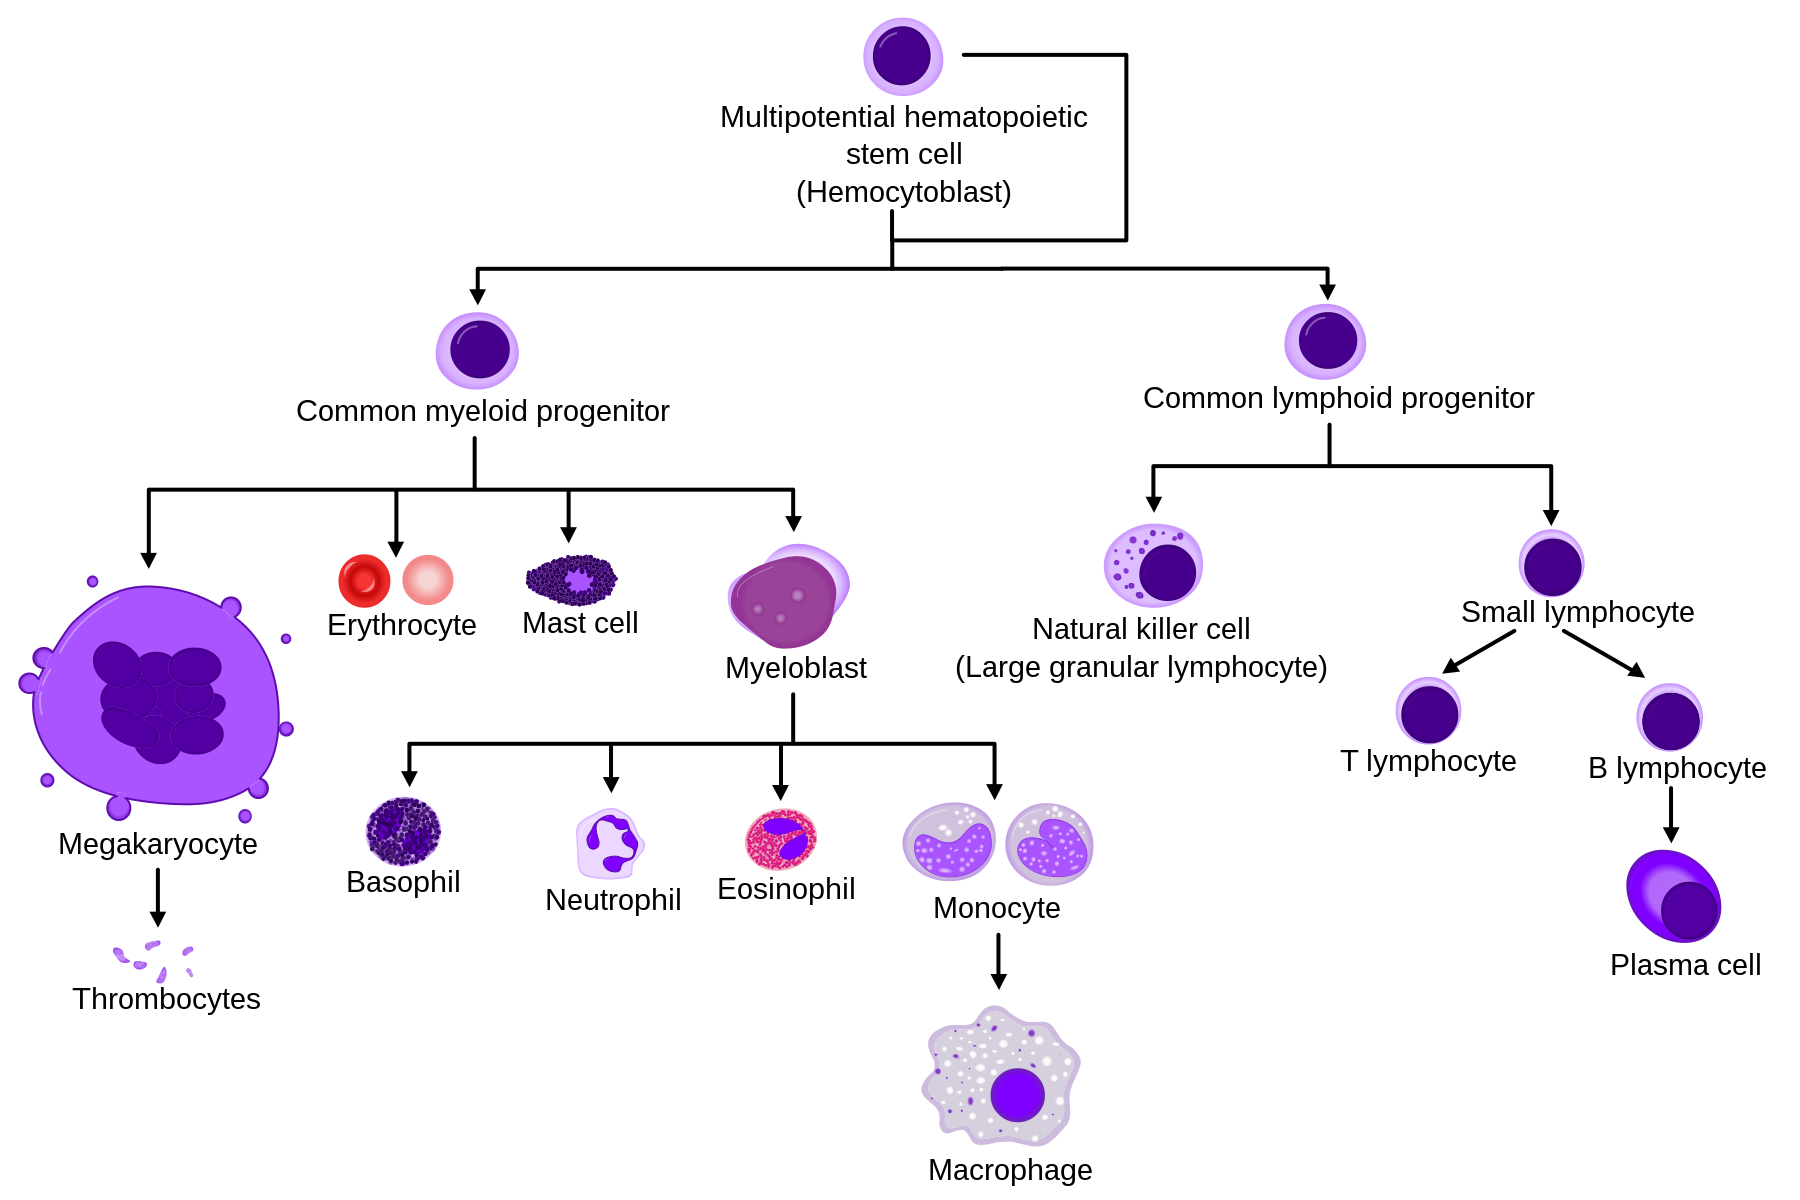
\includegraphics[width=0.7\linewidth]{figures/Inflammation/Hematopoiesis_simple.svg.png} 
        \caption{Overview of the formation of blood cellular components (haematopoiesis). All cellular blood components are derived from pluripotent stem cell root. Image from \href{https://en.wikipedia.org/wiki/File:Hematopoiesis_simple.svg}{Wikimedia}.
        \label{figure:bloodformation}}
    \end{figure}  

Natural killer cells are known large granular lymphocytes (LGL). They also have granules in their cytoplams, but they are not considered to be granulocytes. They have a different root of pluripotent differentiation (figure \ref{figure:bloodformation}), and as such their granules have different functions related to direct killing rather than helping the immune system.

Monocytes develops from the same stem root, and while they occasionally display another type of granule (azurophilic granule), are not classified as granulocytes either. They also have only one nucleus but it shaped is elongated and indented, which might be confused with having several nuclei.

\subsubsection{Neutrophils}

These are the most abundant and are responsible for the phagocytosis of bacteria and other foreign substances. They have a similar role as macrophages, but neutrophils are the first to act and are not professional APCs. They are found in the blood from where they migrate to inflammation sites through a process known as chemotaxis. This involves the detection of a chemical signal (chemoattractant) released by cells at the site of infection. The neutrophil follows the gradient of the chemoattractant until it reaches the site of infection.

\subsubsection{Eosinophils}

They play a role in the body's immune response to parasitic infections, allergies, and asthma. They contain granular structures which are bright red dyed with eosin, hence the name. High levels are correlated with eosinophilic asthma and hypereosinophilic syndrome.

\subsubsection{Basophils}

Basophils are responsible for releasing histamine and other inflammatory molecules in response to allergens, parasites, and other types of foreign substances. Basophils make up less than 1\% of all white blood cells in the body.
        
\subsubsection{Mast cells}

Another type of leukocyte which are found throughout the body, particularly in tissues that are in contact with the external environment like the skin, lungs, and digestive tract. They are involved in the regulation of the immune system. When they are overactive, they can upregulate the immune system too much causing allergies, asthma, and autoimmune disorders.

\subsubsection{Monocytes}

    Monocytes are the largest type of white blood cell and play a role in the phagocytosis of foreign substances. Alongside neutrophils, they belong to the phagocytes group. Monocytes are further subclassified as:

    \begin{itemize}
        
        \item{\textbf{Macrophages}} are large white blood cells that are primarily responsible for phagocytosis. Macrophages also play a key role in presenting antigens to other cells of the immune system, which enables them to launch an appropriate immune response. They are mostly concentrated in the spleen, liver, and lymph nodes. When the proper signaling arrives, they migrate to blood vessels and from there to the inflammation site. Macrophages are further divided into two types:

            \begin{itemize}

                \item{\textbf{M1}} are activated by pro-inflammatory cytokines or \gls{lps}. They produce pro-inflammatory cytokines themselves and kill microbes by phagocytosis or ROS-like substances.
                
                \item{\textbf{M2}} are activated by anti-inflammatory cytokines. These macrophages collaborate in tissue repair.

            \end{itemize}
            
        \item{\textbf{Dendritic cells}} are specialized immune cells that are found primarily in tissues that are in contacts with the external environment, such as the skin, lungs, and intestines. Dendritic cells are known for their ability to capture and process antigens, which they then present to other immune cells in order to activate an immune response. Dendritic cells are particularly important in the initiation of adaptive immune responses,

    \end{itemize}

\subsubsection{Natural killer cells}

\gls{nk} cells identify and destroy human cells. Typically those cells would be infected or cancerous cells presenting an abnormal antigen in the MCH1. But they can also be healthy cells that lack the proper MHC1, such as in transplants from another body, cancer cells that typically display less MHC1, or simply that NK cells can't recognize MCH1 as self due to an autoimmune disorder. Unlike B and T cells, NK cells do not require prior activation which allows them to act very fast preventing further cancer growth or incubation time. They also produce cytokines that help regulate the immune response. On the downside, they do not have memory or clonal expansion capabilities.

\subsubsection{Lymphocytes}

Lymphocytes are involved in the immune response, producing antibodies against foreign substances and attacking infected or cancerous cells. There are divided into further categories:

    \begin{itemize}

        \item[B-lymphocytes] are involved in producing antibodies that will help other leukocytes to recognize and kill the pathogen, or prevent the pathogen to do its function correctly. The basic sub-classification is:

        \begin{itemize}

            \item{\textbf{B-cells}} are both activated by APC and APC themselves, they can help regulate the activity of T-cells, but this is not their main function. They are responsible for producing antibodies. Antibodies are also known as \gls{ig}, and are sub-classified into the following categories:
    
                \begin{itemize}
        
                    \item{\textbf{IgA:}} Found in high concentration in saliva, tears, breast milk, and mucous membranes.
            
                    \item{\textbf{IgD:}} These antibodies are found on the surface of B cells when they exist in the bone marrow and are co-expressed with IgM. But to this day their function is not fully understood.
            
                    \item{\textbf{IgE:}} Bind to allergens such as pollen, animal dander, and food particles, triggering the release of histamine.
            
                    \item{\textbf{IgG:}} Common in the blood and tissue fluids, they have a role in the adaptative immune response. They are also the only type of antibody that cross the placenta from a mother to the fetus, providing temporary immunity.
            
                    \item{\textbf{IgM:}} First to be produced in response to an infection and are effective against general bacteria and viruses.
                
                \end{itemize}
    
            When a B-cell changes producing one Ig to a different one is known as class switching. Later on, we will also talk about lipid mediator class switching, but despise the name, the two concepts are unrelated.
    
            \item{\textbf{Plasma cells}} Are specialized B-cells that can only generate one type of antibody which is triggered by one particular antigen. They serve as a specialized and quick response in current infections and have a short time lifespan.
        
            \item{\textbf{Memory B cells}} are the same as plasma cells, but they have a long time lifespan and provide long-term immunity for years. When memory B cells finally die, you need a memory shot vaccine for their related disease. They can be activated by the pathogen directly, but is more common that they are awakened by memory T cells.        

        \end{itemize}


        \item {T cells} are involved in killing infected cells and regulating the immune system producing cytokines. They are called "T" because they mature in the thymus, but their further sub-classification and function range widely:

        \begin{figure}[ht]
            \centering
                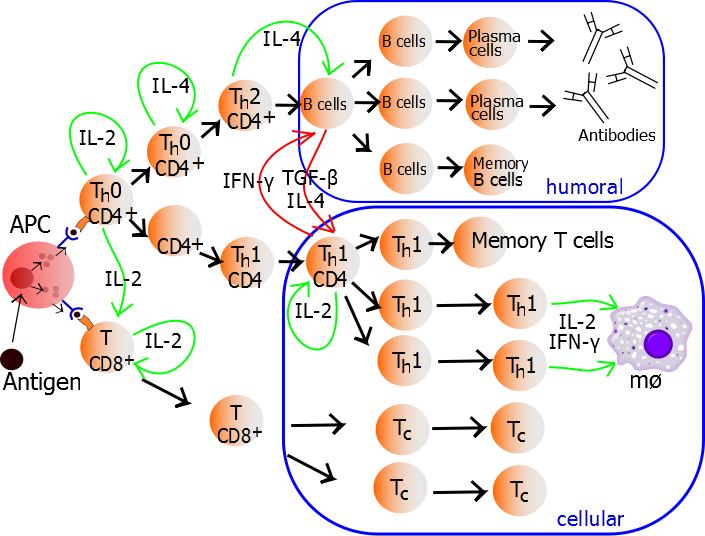
\includegraphics[width=0.5\linewidth]{figures/Inflammation/Lymphocyte_activation.png} 
            \caption{Overview of the T-cells activation and differentiation. Image from \href{https://en.wikiversity.org/wiki/WikiJournal_of_Medicine/Medical_gallery_of_Mikael_H\%C3\%A4ggstr\%C3\%B6m_2014}{"Medical Gallery of Mikael Häggström 2014". WikiJournal of Medicine}}.
            \label{figure:Thell}
        \end{figure}  
    
            \begin{itemize}
    
                \item{\textbf{\gls{th}:}} bind to APC and stimulate the production of antibodies and cytokines. When T-cells are immature they are known as "Th" or "Th0". Then they get activated by APC turning into two main types, "Th1" or "Th2". Th1 cells lead to a cell-mediated response, and Th2 cells lead to a humoral immune response. "Th17" type is a third type that produces IL-17, a pro-inflammatory substance especially good at fighting extracellular pathogens and fungi. THαβ is the fourth type and  provides host immunity against viruses by activating Natural Killer cells. Any Th cell that expresses the CD4 protein, is also known as CD4+ cells.
        
                \item{\textbf{Cytotoxic T cells:}} These cells directly kill infected cells same as NK cells. The cells are known by many other names, including TC, cytotoxic T lymphocyte, CTL, T-killer cell, cytolytic T cell, CD8+ T-cell, and killer T cell, which may cause confusion with other T cell names. Cytotoxic T cells are part of the adaptive immune system and are highly specific in recognizing and attacking infected or abnormal cells that display a specific antigen on their MHC. In contrast, NK cells do not recognize specific antigens, but rather detect and target cells that have decreased expression of normal surface proteins, such as MHC1. Cytotoxic T cells can develop a long-lasting immunological memory after encountering an antigen, allowing for a more rapid and efficient response upon re-exposure.
        
                \item{\textbf{Regulatory T cells:}} These cells help control the immune response by suppressing the activity of other T cells, preventing them from attacking healthy cells.
        
                \item{\textbf{Natural killer T cells:}} Not to be confused with either Cytotoxic T cells (T-killer cells) or Natural Killer cells (NK cells). They can also be CD4+ and CD8+ cells. They recognized microbial lipids and enhance humoral immunity. Upon activation, they produce large quantities of \gls{ifng}, IL-4, and granulocyte-macrophage colony-stimulating factor, IL-2, IL-13, IL-17, IL-21, and \gls{tnfa} among others. Lack of NKT shows autoimmune diseases, autoinflammatory diseases, and cancers.
        
                \item{\textbf{Memory T cells:}} There are 5 types of memory T cells and 3 major ways of activation. They also share some functions with memory B cells. But simplifying their function consists of recognizing previously encounter pathogens and activating the appropriate memory B cells. They actually have a relatively short lifespan and need to be manufactured constantly.
    
            \end{itemize}
        
    \end{itemize}


 

\subsection{Granules}
\label{inf:granules}

Granules are sacs contained in the cytoplasm and contain inflammatory mediators. The two main types of cells that have granules are lymphocytes of the granulocytes class and endothelial cells. In the case of the endothelial cells, granules are stored inside the Weibel–Palade body. Here we list the main inflammatory mediators released from granules during an inflammation process.

\subsubsection{Von Willebrand factor}
\label{in:VonWill}

\gls{vwf} is a protein that plays a key role in the initial stages of clotting by binding to platelets and forming a plug at the site of injury. In an inflammatory process produced by an injury, the most important mechanism is to first stop the bleeding quickly so you don't die. Afterward, other mechanisms will promote vasodilation so the leukocytes can actually go there to do their job. It deficiency might be caused by the most common hereditary blood-clotting disorder in humans \gls{vwd}, which is presented in the form of too much bleeding tendency, such as bruising, nosebleeds, heavy menstrual periods, even severe internal bleeding in the worse cases.

\subsubsection{Selectin}
\label{in:selectin}

Selectins are a family of \gls{cam}. The work of selectin in epithelial cells is slow down leukocyte rolling alongside the interior of blood vessels, and bring it out of the blood vessel so it can go into the source of inflammation and deal with it. There are three subsets:

\begin{itemize}

    \item {\textbf{P-selectin}}. The release of histamine or thrombin in the inflammation sites makes endothelial cells rise P-selectin stored in the cytoplasm up to their cell wall. These are proteins in the shape of "hooks" that catch leucocytes or platelets near the inflammation site.
 
    \item {\textbf{E-selectin}}. Release of IL-1 and TNF-α by macrophages in the inflammation site induces expression of E-selectin on endothelial cells bringing leukocytes inside. They work similarly to P-selectin, but E-selectin takes longer to be activated and is produced and released rather than stored in the cells.
    
    \item {\textbf{L-selectin}} is expressed in leukocytes and they hook to the P/E-selectin expressed in the endothelial cells. L-selectin is also present on the surface of the human embryo and works the same way as with leukocytes facilitating its adhesion to the endometrium.
    
\end{itemize}

\subsubsection{Bradikin}

Bradykinin is a vasodilator, leading to increased blood flow into the affected area. It also increases vascular permeability, allowing inflammatory cells and proteins to move from the bloodstream into the affected tissues. Additionally, bradykinin activates pain receptors, leading to the sensation of pain associated with inflammation.

\subsubsection{Histamine}
\label{in:histamine}

Mast cells and basophils can be activated by IgE and \gls{c3a}. This releases histamine which is an organic nitrogenous compound acting as a chemokine. When this happens, more P-selectin is expressed on the endothelial cells, and at the same time, endothelial cells open up so other leukocytes can migrate to the inflammation site. This process is ilustrated in figure \ref{figure:histamine}.

    \begin{figure}[ht]
        \centering
            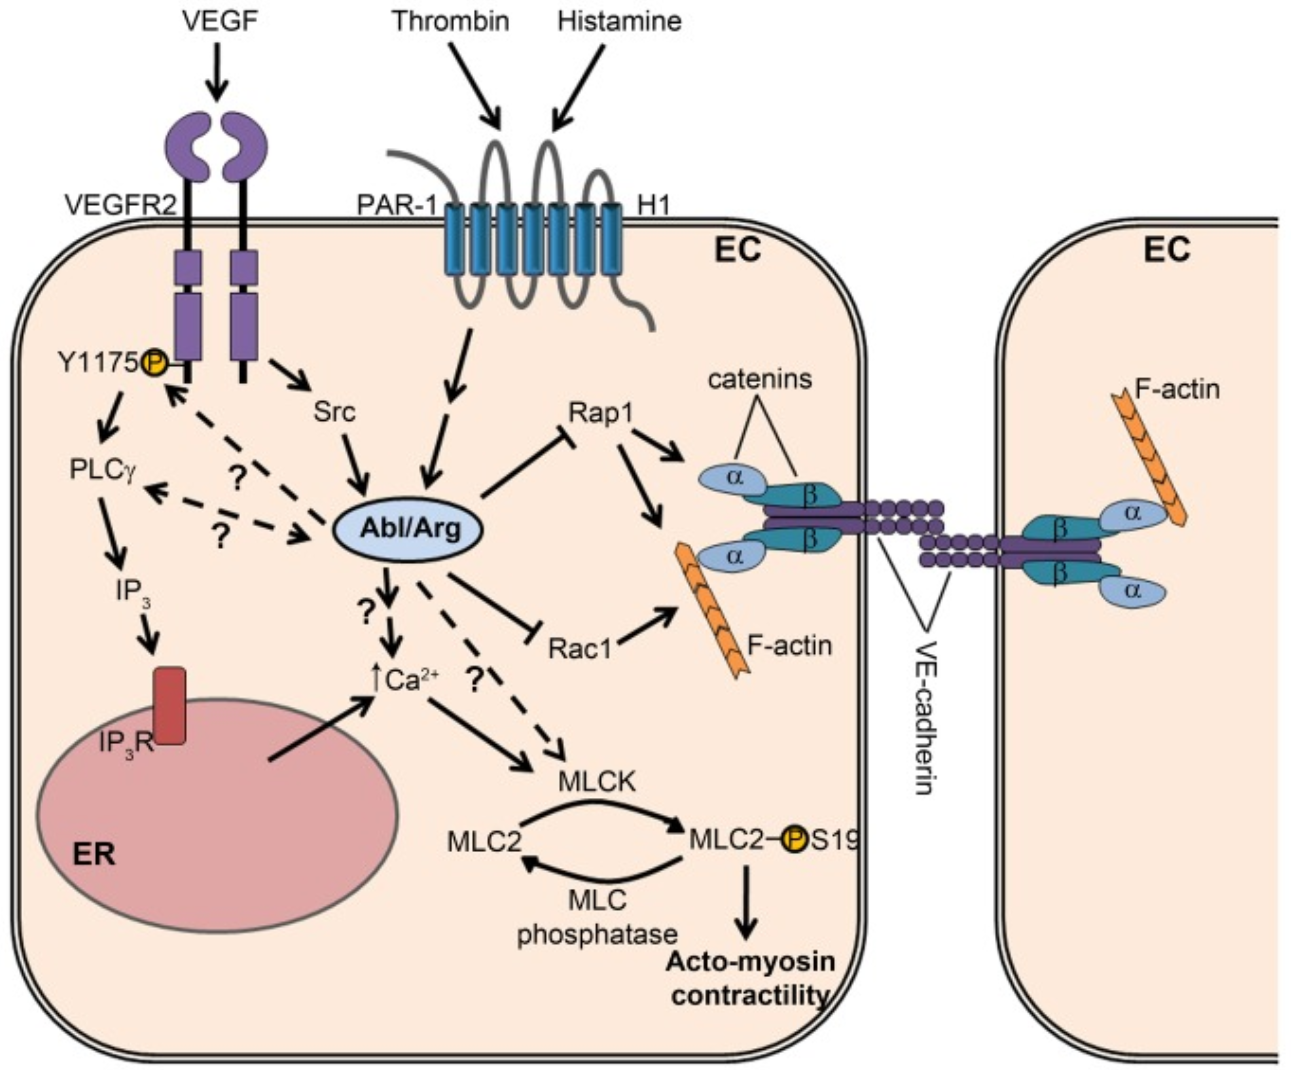
\includegraphics[width=0.5\linewidth]{figures/Inflammation/HistaminPselectin.png} 
        \caption{Overview of the histamine/thrombin cascade signaling which activates PS19 (P-selectin) to migrate up to the cell wall. This mechanism also activates the side chains VE-cadherin to open allowing for leukocytes to abandon the blood stream. Image from \href{https://www.nature.com/articles/nature13479}{"XXX UNKNOWN!"}.
        \label{figure:histamine}}
    \end{figure}  

However, histamine is also released when allergens bind to mast-cell-bound IgE antibodies sites. This is commonly known as an allergy and is the mechanism that can make your life miserable in the form of  bronchial smooth muscle contraction, urinary bladder contractions, vasodilation, visceral hypersensitivity, itch perception, urticaria, sneezing, hyper-secretion from glandular tissue, and  nasal congestion due to vascular engorgement. This is typically alleviated by the use of antihistamines medication.

In the worst-case scenario, histamine can lead to an anaphylactic shock which causes dead typically by collapsing the respiratory airways.

\subsubsection{Cytokines}

A description of the different types of cytokines can be found in section \ref{ref:inflammationCytokines}.
   
\subsubsection{Eicosanoids / Arachidonic acid}
\label{eicosanoids}

   Eicosanoids are a family of lipids that acts like hormones. They derive from arachidonic acid, and sometimes the two names are used interchangeably. Arachidonic acid is released during cell damage. Arachidonic acid is found in meat and eggs from animals that have free range and are able to exercise and move freely, as such, a lack of proper quality items in the diet can't initiate proper resolution in the inflammation cycle. They are suppressed by steroids and promoted by tissue injuries, thrombin, bradykinin, and epinephrine. An overview of the actions of eicosanoids can be seen in figure \ref{figure:Eicosanoids1}. Details regarding eicosanoids are discussed later in the sections \ref{arcachonidacidsPRO} and \ref{arcachonidacids}.
    
    \begin{figure}[ht]
        \centering
            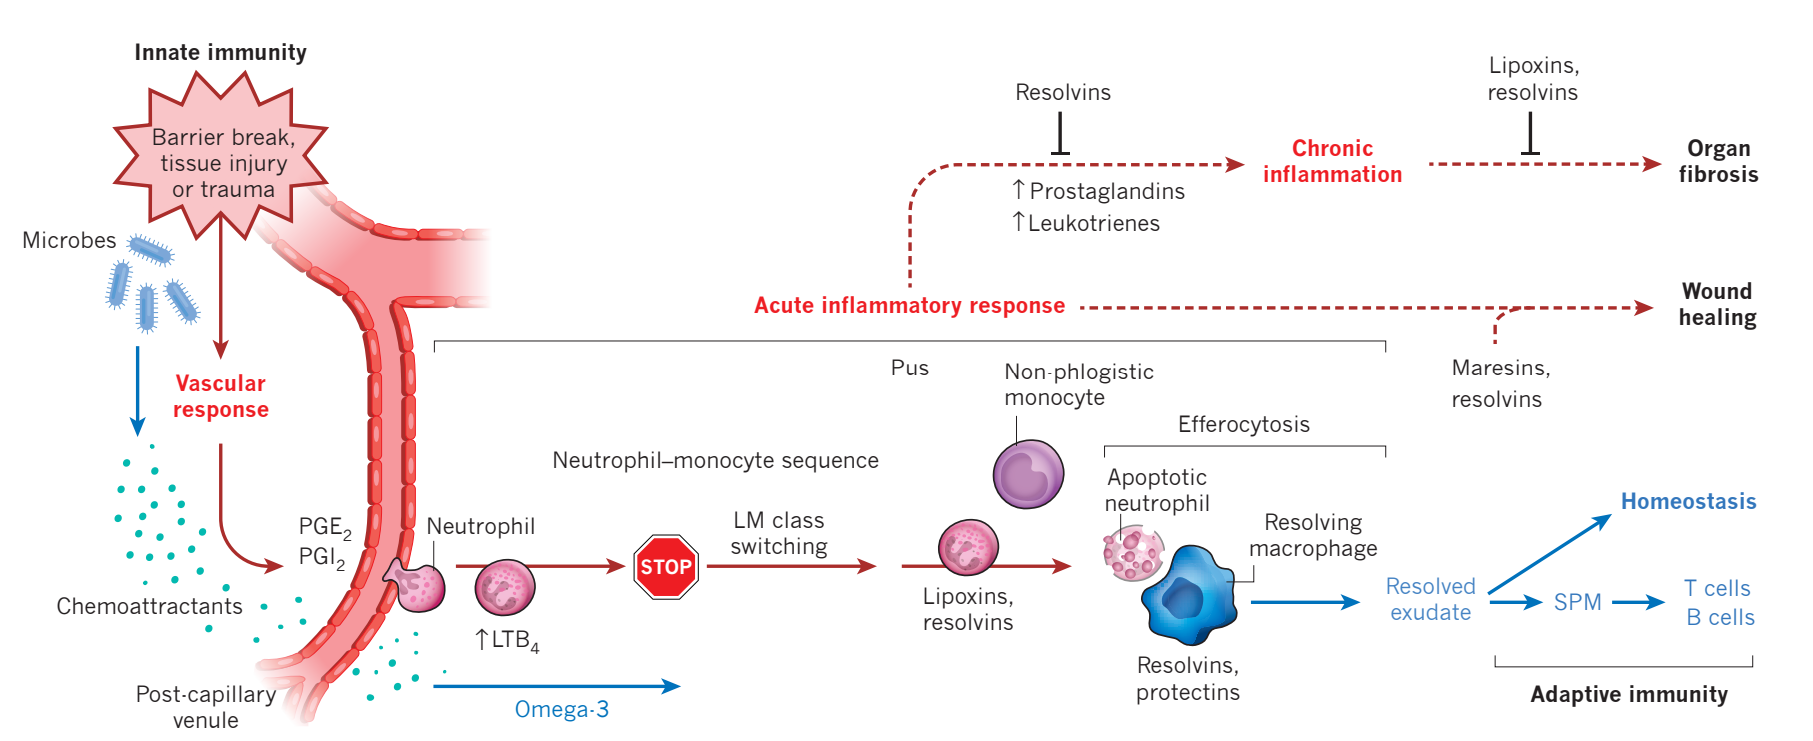
\includegraphics[width=0.9\linewidth]{figures/Inflammation/nature1.png} 
        \caption{Overview of the roles of lipid mediators in vascular and leukocyte response, from the initiation of inflammation to the resolution of the event. Image from \href{https://www.nature.com/articles/nature13479}{"Pro-resolving lipid mediators are leads for resolution physiology"}}.
        \label{figure:Eicosanoids1}
    \end{figure}  

\subsubsection{Serotonin}

Serotonin is a well-known neurotransmitter better known for regulating mood, appetite, and sleep. But it also controls the activation and proliferation of T and B cells. Overall, the function of serotonin in immunity is complex and not fully understood yet, but some studies suggest that serotonin may have a protective role against infections \cite{Roumier2019}.

\subsection{Complement system}

The complement system is a collection 32 of proteins that can kill bacteria directly, or enhance other cells in the immune system via opsonization or chemotaxis production. The functioning of the complement system is a very beautiful topic that involves the complex synchronization of proteins working together like cogs in a machine. Unfortunately is beyond the scope of this document. Here we are just going to list a simplification of the reactions present in the 3 possible pathways, highlighting the proteins important in inflammation that are mentioned in this document.

\subsubsection{Initiation}

When a couple of IgG, or a single IgM, are attached to a bacteria, is possible that by random chance a C1 protein gets attached to these antibodies. If this happens, the complement system becomes initiated.

\subsubsection{Activation}

The C1 protein has two main parts, the C1q and C1rs. C1rs is attached to the Igs, while C1q can cleave other proteins. C1q cleaves C2 making C2a and C2b, and also cleaves C4 making C4a and C4b. C4b and C2a bind together making the C4bC2a complex, which cleaves C3 making C3a and C3b. C3b binds with C4bC2a making the "C4b2a3b Convertase". This attaches to the bacteria. When this finally occurs, then it is said that the complement system is activated.

\subsubsection{Amplification}

C3b can also bind to another C3b and attach to the bacteria. This also can cleave C3 proteins, which translates into an exponential growth of the C3bC3b complex attached to the bacteria and C3a flooding the bloodstream. C3a activates basophils into releasing histamine (section \ref{in:histamine}), which promotes the expression of P-selectin, which promotes the traveling of neutrophils into the inflammation site.

\subsubsection{Termination}

C4b2a3b Convertase can also cleave C5 into C5a and C5b. C5a creates a chemotaxis gradient for neutrophils which kill the bacteria. Furthermore, neutrophils and other immune cells catch the bacteria by attaching to C3bC3b which is already attached to the bacteria wall. Here, C1q also stimulate the neutrophils to start the destruction of whatever they just grabbed. As C1q is supposed to only be attached to pathogens, this prevents them from destroying healthy cells accidentally caught by neutrophils.

The complement system can also terminate bacteria by itself forming the MAC complex, which consists of several other proteins that attach to C5b, which literally makes a hole in the bacteria wall of approximately 25 times the diameter of water molecules, allowing the insides of the bacteria to leak out.

%*****************************************
\section{Immunology advance concepts}
%*****************************************

Now that the basics of immunology have been explained, we can dive into more complex mechanism that fully explain the inflammation cycle.

\subsection{Type 1 vs Type 2 immune response}

The Type 1 immune response is characterized by the activation of Th1 cells which secrete cytokines that stimulate the production of antibodies by B cells and activation of cytotoxic T cells. It is primarily effective against intracellular pathogens such as viruses and bacteria, and the development of cell-mediated immunity. Type 1 immunity response is mainly mediated by Th1, cytotoxic T-lymphocytes, and NK cells. Type 1 immunity implies the production of pro-inflammatory cytokines and IgG and IgM antibodies.

The Type 2 immune response involves the activation of Th2 cells which secrete cytokines that activate eosinophils, basophils, and mast cells, causing allergic inflammatory responses and increased production of antibodies by B cells. It is primarily effective against extracellular pathogens such as parasites, worms, and allergens and the development of humoral immunity. Type 2 immunity response is mainly mediated by Th2 cells, eosinophils, basophils, and mast cells. Type 2 immunity generally implies the production of anti-inflammatory cytokines but also involve both types such as in the case of IL-5 which promote allergic reactions. It also mainly promotes IgA and IgE.


\subsection{Nitric Oxide}
\label{in:NO}

\ch{NO} is a free radical generated by phagocytes and is toxic to bacteria and some parasites, as well as to many human cells, leading to apoptosis. The damage to human cells is intentional and is believed to be used as a way of getting rid quickly of cells that are promoting pro-inflammation mechanisms. Is activated by \gls{ifng} and TGFα, and is suppressed by IL-4, IL-10, and TGFβ.

\subsection{JAK-STAT pathway}
\label{in:JAKSTAT}

\gls{jakstat} pathway are related to endocrinology and its main function is to couple with a receptor that attaches to the grown hormone and brings it inside the cell. However, the receptor of JAK-STAT can also bind to several cytokines. In particular IL-2, IL-6, and interferons.

What is important to understand for the scope of this document is that the JAK portion function by phosphorylating each other, which phosphorylate the STAT part, which goes into the cell nucleus, which will promote gene transcription, which promotes protein translation.

\subsection{Pro-inflammatory Eicosanoids}
\label{arcachonidacidsPRO}

In section \ref{eicosanoids} we introduced how eicosanoids are included inside granules. Here we are going to expand on them and list the pro-inflammation ones.

\subsubsection{Thromboxane}
\label{in:Thromboxane}

They work in the first stage of tissue damage by acting as a pro-coagulation agent, a vasoconstrictor, a hypertensive agent, and facilitating platelet aggregation.

\subsubsection{Prostaglandins}

\gls{pg} are a complex family of eicosanoids which act both as pro-inflammation when the recruitment of the immune system is needed, and anti-inflammatory when the damage has been resolved. There are four different subclasses:

    \begin{itemize}
        \item {\textbf{PGD2:}} Produced by mast cells and is primarily involved in allergic responses.
        \item {\textbf{PGE2:}} It is responsible for the pain and fever associated with inflammation.
        \item {\textbf{PGF2α:}} Involved in the contraction of the smooth muscle in the uterus.
        \item {\textbf{PGI2:}} Produced by the endothelial cells lining blood vessels and plays a role in vasodilation. It shares PGH2 precursors with Thromboxane which is a vasoconstrictor. You can't either have vasodilation or vasoconstriction, and both pathways are never active at the same time. Vasoconstriction reaction however occurs much more rapidly.
    \end{itemize}

\subsubsection{Leukotrienes}
\label{in:lt}

\gls{lt} are both autocrine signaling and paracrine signaling. They serve to regulate immune responses bringing neutrophils. The LTC4, LTD4, LTE4, and LTF4 prolonged slow contraction of smooth muscle and have a major bronchoconstrictor role in asthma. \gls{nsaids} block prostaglandins but promote leukotrienes, prostaglandins are initially pro-inflammatory but later on, switch to anti-inflammation, while leukotrienes are always pro-inflammation. This is the reason why NSAIDs are not always recommended for mild inflammations, and as long as the pain is bearable, is better in the long run to avoid its use. Especially if side effects on the liver and stomach are taken into consideration.

\subsection{Specialized pro-resolving mediators}
\label{arcachonidacids}
\label{in:spm}

Again, in section \ref{eicosanoids} we introduced how eicosanoids are included inside granules. Here we are going to talk about the switch from a pro-inflammation state to an anti-inflammatory effect which leads to the resolution of inflammation. These are known as specialized pro-resolving mediators (SPMs).

        \begin{figure}[h!]
            \centering
                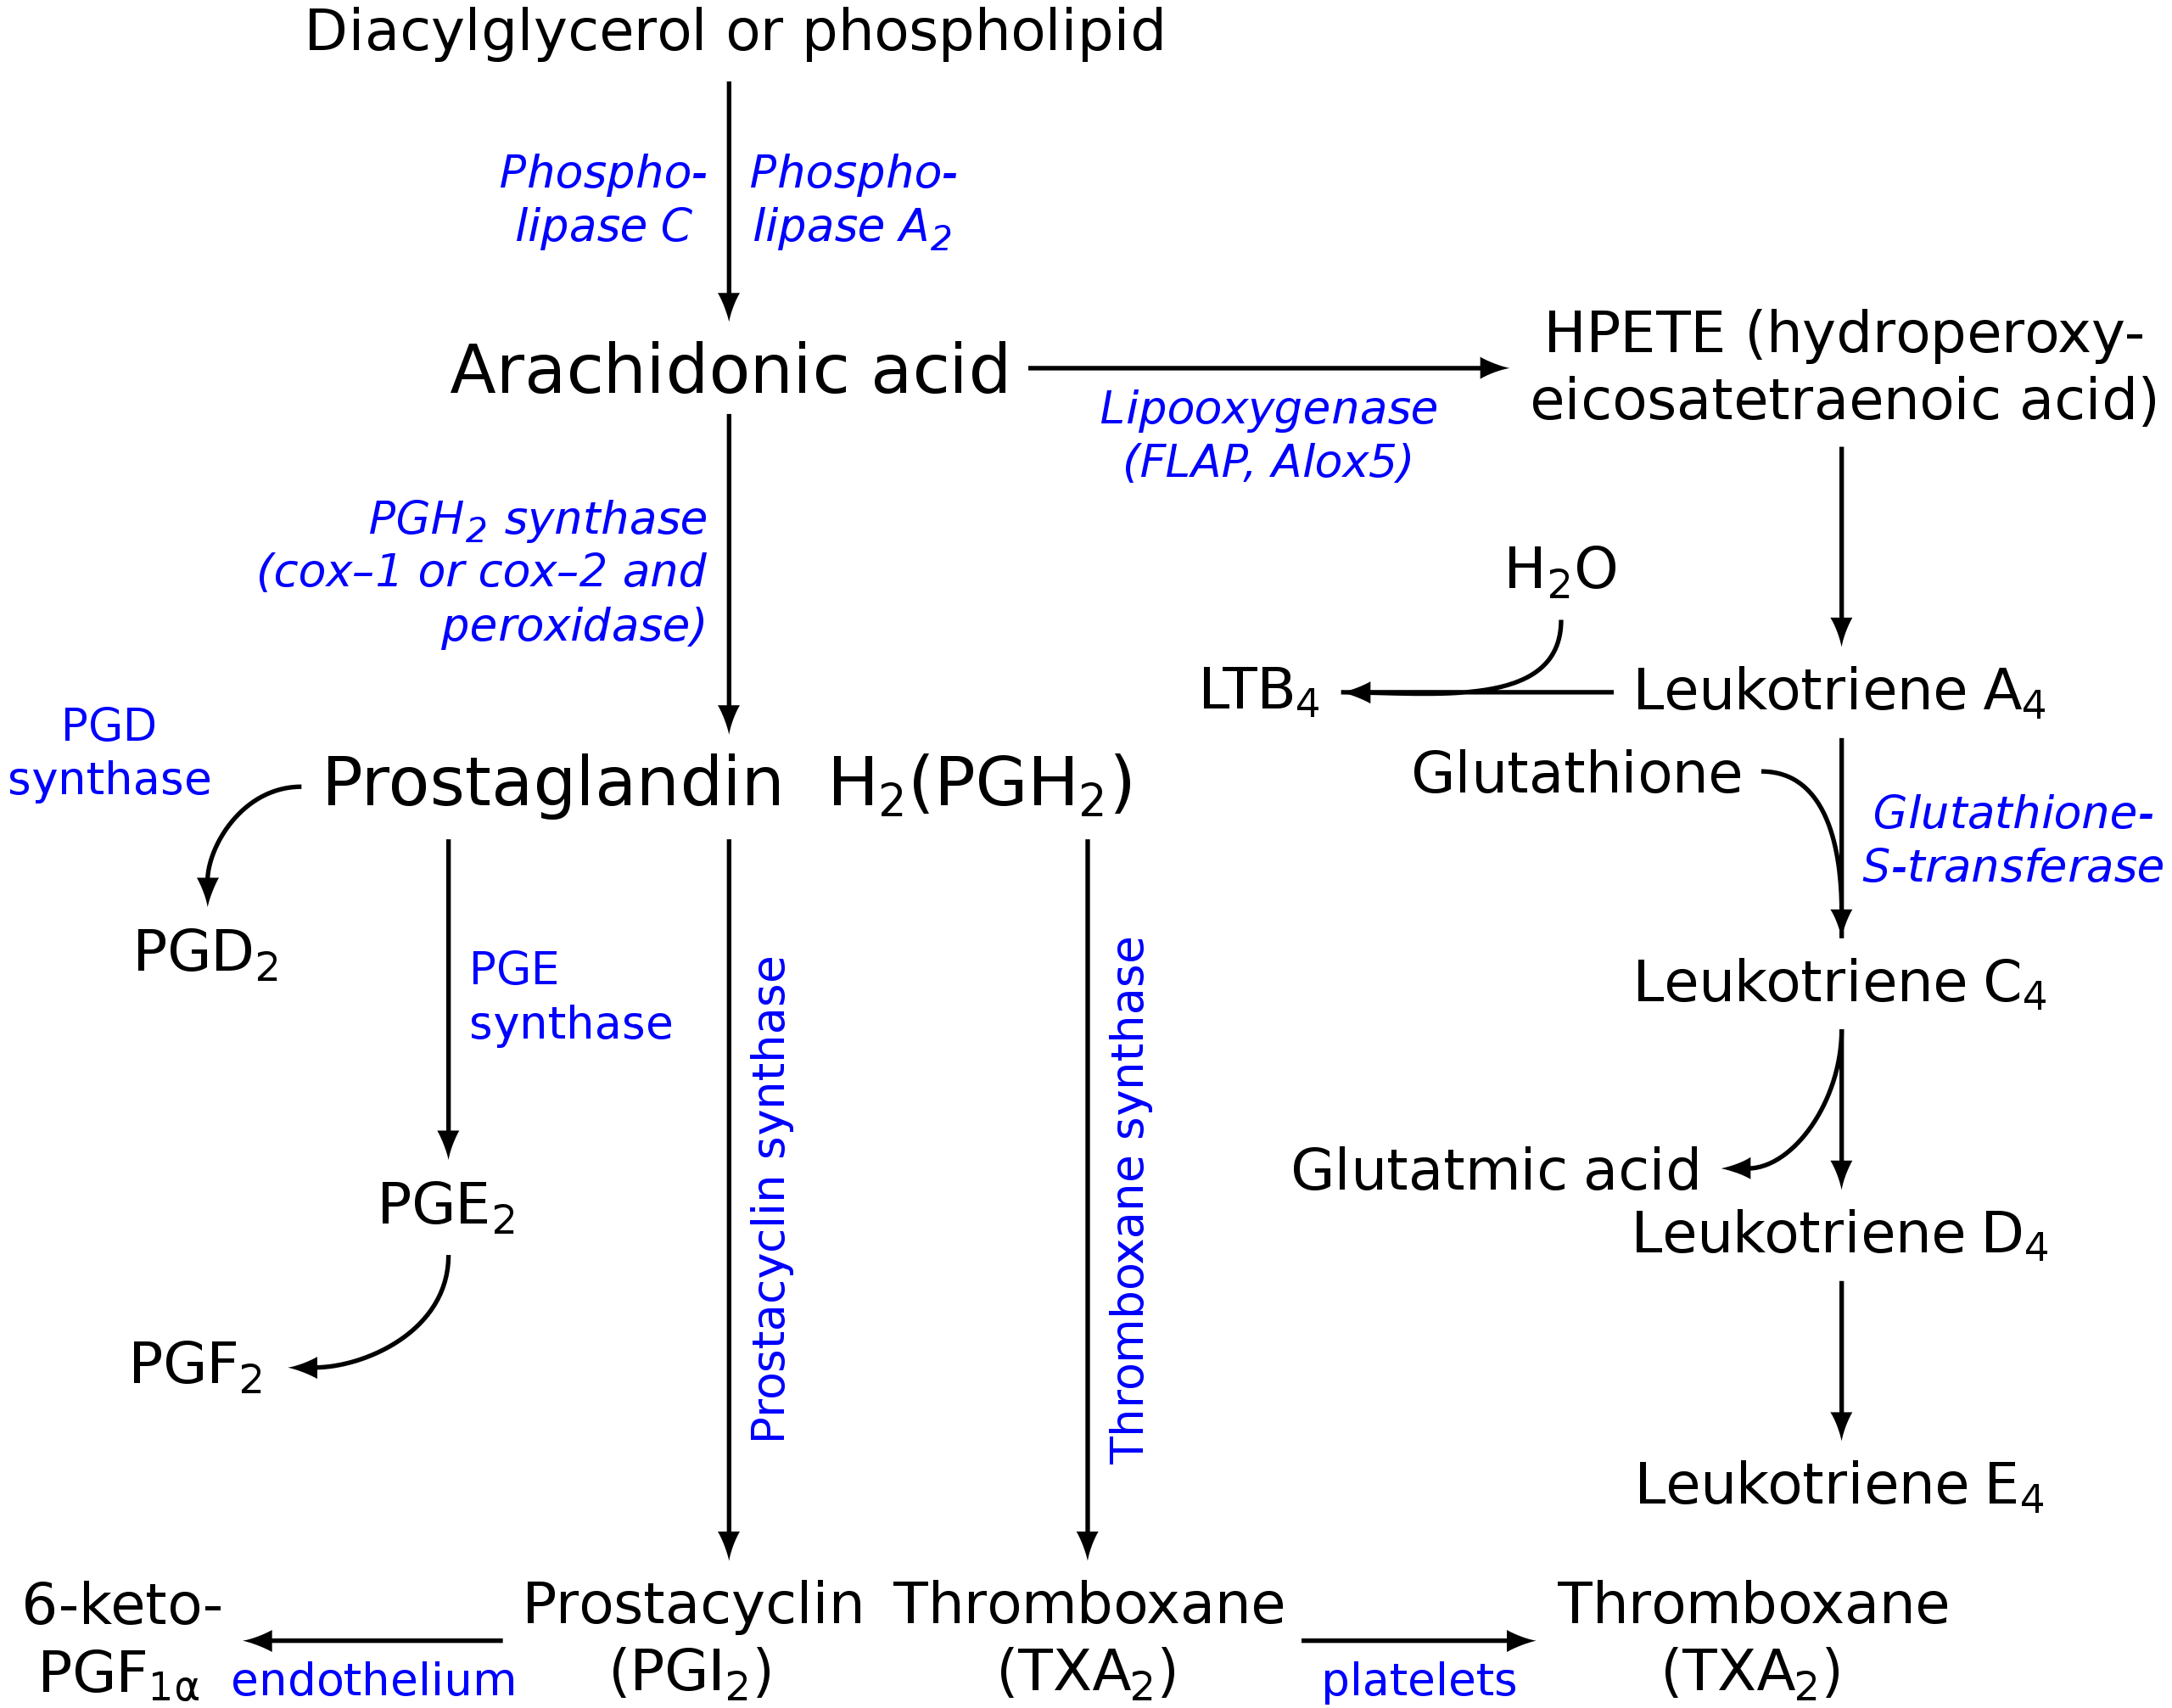
\includegraphics[width=0.7\linewidth]{figures/Inflammation/2560px-Eicosanoid_synthesis.svg.png} 
            \caption{Overview of the prostaglandin pathways. Image from \href{https://en.wikipedia.org/wiki/File:Eicosanoid_synthesis.svg}{Wikipedia}}.
            \label{figure:Phell}
        \end{figure}  


\subsubsection{Lipoxin}

Lipoxins reverse the actions of the pro-inflammatory mediators and initiate tissue repair response \cite{Basil2015}. Among many other things, they inhibit chemotaxis, transmigration, superoxide generation, NF-κB activation, generation of pro-inflammatory cytokines, suppress the production of IgM and IgG antibodies, reduce the perception of pain due to inflammation, induce the production of elements that neutralize oxidative stress and oxidant-induced tissue damage and block the actions of some leukotrienes. \cite{Sharmawalia2015}

\subsubsection{Resolvins}

Resolvins play an important role in resolving inflammation by promoting the clearance of cellular debris, bacteria, and other inflammatory mediators. They also inhibit neutrophil recruitment, decrease pro-inflammatory cytokine production, and promote tissue repair and regeneration \cite{Moro2016}. The importance of resolvins lies in their ability to control the duration and intensity of inflammation, which is crucial for preventing the development of chronic inflammatory diseases.

        \begin{figure}[h!]
            \centering
                \includegraphics[width=0.8\linewidth]{figures/Inflammation/nihms646633f2.jpg}
            \caption{Overview of EPA and DHA conversion into resolvins, protectins, and maresins. Image from \href{https://www.nature.com/articles/nature13479}{"Pro-resolving lipid mediators are leads for resolution physiology"}}.
        \label{figure:Eicosanoids2}
        \end{figure}  

They are formed from the metabolism of omega-3 polyunsaturated fatty acids, in particular, \gls{epa} and \gls{dha} (figure \ref{figure:Eicosanoids2}). Humans convert \gls{ala} to EPA very inefficiently, so is recommended to take food rich in EPA directly such as salmon, mackerel, herring, cod liver, some algae, and human milk. DHA can be converted from EPA, but is recommended to also take DHA-rich food such as salmon, caviar, anchovies, mackerel, or herrings.

\subsubsection{Protectins / Neuroprotectins }

Protectins reduce inflammation induced by oxidative stress and inhibit the pro-apoptotic signal. Can potentially protect respiratory cells from viral infections. Blocks formation of pro-inflammatory prostaglandins, inhibits platelet-aggregating by thromboxane thus blocking the platelet aggregation responses such as those described for \textit{S. Aureus} in section \ref{stahp:coagulase}, and stimulate the efferocytosis \cite{Lagarde2014, Serhan2015}.

\subsubsection{Maresins}

Its name derives from \textit{\textbf{MA}crophage mediator in \textbf{RES}olving \textbf{IN}flammation}. They are involved in resolving inflammation and allergic reactions, wound healing, apoptotic human neutrophils by human macrophages, reduced lung inflammation, suppress the production of IL-5 and IL-13, and reduce the production of LTB4.

\subsubsection{Eoxins}

Eoxins are proinflammatory eicosanoids first described in 2008 \cite{Feltenmark2008} which are suggested to contribute to the inflammation of airways during allergies and some cancers \cite{Claesson2009}. They still have an unknown function in human physiology or pathology. But their production is stimulated in eosinophils by pro-inflammatory mediators PD2, LTC4, and IL-5.

\subsection{APR}

\gls{apr} are proteins that are produced by the liver and are high in plasma when there is a cause of inflammation or infection and correlate with disease activity. They are generated in response to IL-6. They go down when the cause of inflammation or infection has been resolved. However they have no diagnostic value; it is just an indicator that something wrong is going on, but there are too many diseases that cause APR to be high.

\subsubsection{CRP}

\gls{crp} is a type of APR. It is called "C" because it was first discovered reacting with the C-polysaccharide of the Capsule of \textit{Streptococcus pneumoniae}. It attaches to bacteria or dying cells which promotes phagocytosis by macrophages. It also interacts with C1q and enhances its ability to bind to pathogens, and is also believed to interact with C3; although the mechanisms of interaction between CRP and the complement system are not fully understood. It increases very rapidly and falls very rapidly as it mean half-life is barely 7 hours. Increased CRP is correlated with an increased risk of cardiovascular disease (CD) only if the patient history also correlates with CD.

\subsubsection{ESR}

The \gls{esr} is another acute phase reactant that is used to measure inflammation. It measures how quickly red blood cells clump together and settle to the bottom of a test tube. Inflammation causes the blood to become thicker and stickier, which causes the red blood cells to settle faster. In opposition to CRP, ESR still remains high after the resolution of the inflammation or infection and takes up to 7 days to regress to normal levels.


\subsection{Interleukins}
\label{in:interleukins}

% https://www.researchgate.net/figure/Role-of-interleukins-in-each-dimension-of-rheumatoid-arthritis_fig1_311472701

% https://www.researchgate.net/figure/Interleukins-involved-in-acute-and-chronic-inflammatory-responses-31-30_fig1_341541401

% https://www.researchgate.net/figure/Cytokines-profile-in-viral-infections-The-immune-response-against-viruses-initiates_fig3_330948439

% Table

% Accute VS Chronic response
% +/- immune response
% +/- inflammation
% + Cell grow
% Chemotactic
% Pyrogenic
% Released by X leukocytes
% Activate X leukocytes

% Table Agonists or Antagonists


% Figure: https://roami.ro/wp-content/uploads/2019/12/149-162_Art_Ovidiu_Farc__Victor_Cristea_web.pdf

% https://www.ncbi.nlm.nih.gov/books/NBK499840/

    \begin{figure}[h!]
        \centering
            \includegraphics[width=0.8\linewidth]{figures/Inflammation/ILHell.png} 
        \caption{Overview of all interleukins affecting tumoral growth. Image reproduced from "PRO-AND ANTITUMOR ROLE OF THE INTERLEUKINS 1 TO 41" \cite{bigTumorFigureBook}}.
        \label{figure:ilhell}
    \end{figure}

Interleukin is a type of cytokine used both by the immune system and for therapeutic purposes. There are more than 50 interleukins encoded in the human genome, with several subtypes and variants. While interleukins mostly have a beneficial effect, some of them can also contribute to unwanted inflammation, autoimmune diseases, and cancer. They can stimulate or inhibit the proliferation, differentiation, activation, migration, and survival of white blood cells or other immune cells, as well as modulate the production of antibodies, chemokines, or other mediators.

The number of each interleukin is arbitrary and might lead to confusion. For example, Interleukin 1 family members includes IL-1α, IL-1β, IL-18, IL-33, IL-36α, IL-36β, IL-36γ, IL-36ra, IL-37, and IL-38. It must be taken as a unique ID with no other meaning. Here we are going to explain the function of the ILs present in the Olink panel.

The difference between interleukins can be summarized by whether they are pro or anti-inflammatory, the type of immune cells with which they interact, the type of immune cells or other human cells that produce them, and their secondary effects on the body. Individually, interleukins are very easy to understand. But their complex interactions with each other, and with other parts of the immune system make them very difficult to visualize and keep track as can be exemplified in figure \ref{figure:ilhell} and table \ref{table:ilhell}.

% Please add the following required packages to your document preamble:
% \usepackage[table,xcdraw]{xcolor}
% If you use beamer only pass "xcolor=table" option, i.e. \documentclass[xcolor=table]{beamer}

\begin{sidewaystable}[h!]% <===============================================
%\begin{table}[ht]
    \caption{Overview of all interleukins explained in this document}
    \label{table:ilhell}
    \renewcommand{\arraystretch}{1.7}
    \scalebox{0.5}{
    \centering
    \begin{tabular}{|
>{\columncolor[HTML]{FFCE93}}c c
>{\columncolor[HTML]{FBDBB5}}c ccc|}
\hline
\cellcolor[HTML]{C0C0C0}\textbf{ID}                 & \cellcolor[HTML]{C0C0C0}\textbf{Type} & \cellcolor[HTML]{C0C0C0}\textbf{Chemotactic}     & \cellcolor[HTML]{C0C0C0}\textbf{Producers}                                                                      & \cellcolor[HTML]{C0C0C0}\textbf{Targets}                                                                           & \cellcolor[HTML]{C0C0C0}\textbf{Main}      \\ \hline
\multicolumn{1}{|c|}{\cellcolor[HTML]{FFCE93}IL-1}  & \cellcolor[HTML]{FFCCC9}Pro           & \multicolumn{1}{c|}{\cellcolor[HTML]{BCFBBB}Yes} & \multicolumn{1}{c|}{Dendritic cells, Macrophages, Monocytes, T-cells}                                           & \multicolumn{1}{c|}{Pro-inflammation proteins, PGE2}                                                               & Fever, pro-apoptosis, and pro-inflammation \\
\multicolumn{1}{|c|}{\cellcolor[HTML]{FFCE93}IL-2}  & \cellcolor[HTML]{FFCCC9}Pro           & \multicolumn{1}{c|}{\cellcolor[HTML]{FBDBB5}No}  & \multicolumn{1}{c|}{NK cells, T-cells}                                                                          & \multicolumn{1}{c|}{NK cells, T-cells}                                                                             & Increases immune activity                  \\
\multicolumn{1}{|c|}{\cellcolor[HTML]{FFCE93}IL-4}  & \cellcolor[HTML]{96FFFB}Anti          & \multicolumn{1}{c|}{\cellcolor[HTML]{FBDBB5}No}  & \multicolumn{1}{c|}{Basophils, Eosinophils, Mast cells, Th2}                                                    & \multicolumn{1}{c|}{M1, Th0, Th2}                                                                                  & Make Th2 and anti-inflammation             \\
\multicolumn{1}{|c|}{\cellcolor[HTML]{FFCE93}IL-5}  & \cellcolor[HTML]{FFFFC7}Both          & \multicolumn{1}{c|}{\cellcolor[HTML]{BCFBBB}Yes} & \multicolumn{1}{c|}{Eosinophils, Mast cells, Th2}                                                               & \multicolumn{1}{c|}{Eosinophils}                                                                                   & Allergic rhinitis and asthma               \\ \hline
\multicolumn{1}{|c|}{\cellcolor[HTML]{FFCE93}IL-6}  & \cellcolor[HTML]{FFFFC7}Both          & \multicolumn{1}{c|}{\cellcolor[HTML]{BCFBBB}Yes} & \multicolumn{1}{c|}{Macrophages}                                                                                & \multicolumn{1}{c|}{B-cells, Neutrophils, T-cells}                                                                 & Fever and Autoimmune                       \\
\multicolumn{1}{|c|}{\cellcolor[HTML]{FFCE93}IL-7}  & Neither                               & \multicolumn{1}{c|}{\cellcolor[HTML]{FBDBB5}No}  & \multicolumn{1}{c|}{Stem cells / Dendritic cells /  Keratinocytes, Hepatocytes, Epithelial cells}               & \multicolumn{1}{c|}{T-cells}                                                                                       & T-cell regulator                           \\
\multicolumn{1}{|c|}{\cellcolor[HTML]{FFCE93}IL-8}  & \cellcolor[HTML]{FFCCC9}Pro           & \multicolumn{1}{c|}{\cellcolor[HTML]{BCFBBB}Yes} & \multicolumn{1}{c|}{Macrophages / Endothelial cells, Epithelial cells, Smooth muscle cells}                     & \multicolumn{1}{c|}{Neutrophils}                                                                                   & CAM activator                              \\
\multicolumn{1}{|c|}{\cellcolor[HTML]{FFCE93}IL-10} & \cellcolor[HTML]{96FFFB}Anti          & \multicolumn{1}{c|}{\cellcolor[HTML]{FBDBB5}No}  & \multicolumn{1}{c|}{Monocytes}                                                                                  & \multicolumn{1}{c|}{Macrophages, B cells, Th1}                                                                     & Anti-inflammation                          \\ \hline
\multicolumn{1}{|c|}{\cellcolor[HTML]{FFCE93}IL-12} & \cellcolor[HTML]{FFCCC9}Pro           & \multicolumn{1}{c|}{\cellcolor[HTML]{FBDBB5}No}  & \multicolumn{1}{c|}{B-cells, Dendritic cells, Macrophages, Neutrophils}                                         & \multicolumn{1}{c|}{NK cells, T-cells}                                                                             & Kill                                       \\
\multicolumn{1}{|c|}{\cellcolor[HTML]{FFCE93}IL-13} & \cellcolor[HTML]{96FFFB}Anti          & \multicolumn{1}{c|}{\cellcolor[HTML]{FBDBB5}No}  & \multicolumn{1}{c|}{Basophils, Eosinophils, Mast cells, NKT cells, Th2}                                         & \multicolumn{1}{c|}{Th0, Th2 and M1}                                                                               & Anti-inflammation and Allergies            \\
\multicolumn{1}{|c|}{\cellcolor[HTML]{FFCE93}IL-15} & \cellcolor[HTML]{FFCCC9}Pro           & \multicolumn{1}{c|}{\cellcolor[HTML]{FBDBB5}No}  & \multicolumn{1}{c|}{Dendritic cells, Macrophages, Monocytes / Fibroblasts, Keratinocytes, Myocyte, Nerve cells} & \multicolumn{1}{c|}{NK cells, Innate lymphoid cells}                                                               & Increases immune activity and survival     \\
\multicolumn{1}{|c|}{\cellcolor[HTML]{FFCE93}IL-17} & \cellcolor[HTML]{FFCCC9}Pro           & \multicolumn{1}{c|}{\cellcolor[HTML]{FBDBB5}No}  & \multicolumn{1}{c|}{Th17}                                                                                       & \multicolumn{1}{c|}{B-cells, Monocytes, Neutrophils, T-cells /  Epithelial cells, Endothelial cells,  Fibroblasts} & Increases pro-inflammatory cytokines       \\ \hline
\multicolumn{1}{|c|}{\cellcolor[HTML]{FFCE93}IL-18} & \cellcolor[HTML]{FFCCC9}Pro           & \multicolumn{1}{c|}{\cellcolor[HTML]{FBDBB5}No}  & \multicolumn{1}{c|}{Several}                                                                                    & \multicolumn{1}{c|}{Several}                                                                                       & Type 1 immunity                            \\
\multicolumn{1}{|c|}{\cellcolor[HTML]{FFCE93}IL-20} & \cellcolor[HTML]{FFCCC9}Pro           & \multicolumn{1}{c|}{\cellcolor[HTML]{BCFBBB}Yes} & \multicolumn{1}{c|}{Dendritic cells, Granulocytes, Monocytes}                                                   & \multicolumn{1}{c|}{Adipocytes, Endothelial cells, Keratinocytes}                                                  & Healing                                    \\
\multicolumn{1}{|c|}{\cellcolor[HTML]{FFCE93}IL-22} & Neither                               & \multicolumn{1}{c|}{\cellcolor[HTML]{FBDBB5}No}  & \multicolumn{1}{c|}{Macrophages, Neutrophils, NKT cells, Th1, Th17}                                             & \multicolumn{1}{c|}{Several}                                                                                       & Healing and germicidal                     \\
\multicolumn{1}{|c|}{\cellcolor[HTML]{FFCE93}IL-24} & \cellcolor[HTML]{FFCCC9}Pro           & \multicolumn{1}{c|}{\cellcolor[HTML]{FBDBB5}No}  & \multicolumn{1}{c|}{Macrophages, Monocytes, Th2}                                                                & \multicolumn{1}{c|}{Several}                                                                                       & Anti-healing and Anti-cancer               \\ \hline
\multicolumn{1}{|c|}{\cellcolor[HTML]{FFCE93}IL-33} & \cellcolor[HTML]{96FFFB}Anti          & \multicolumn{1}{c|}{\cellcolor[HTML]{FBDBB5}No}  & \multicolumn{1}{c|}{Several}                                                                                    & \multicolumn{1}{c|}{Mast cells, Th2}                                                                               & Promotes Th2 cytokines                     \\ \hline
\end{tabular}
    }
%\end{table}
\end{sidewaystable}

\subsubsection{IL-1}
\label{in:IL1}

\gls{il1} is a cytokine that is involved in regulating the immune response and inflammation. It is produced by macrophages, monocytes, dendritic cells, and certain types of T cells. It is involved in both innate and adaptive immune responses and plays a key role in the body's defense against pathogens.

Activates and promote the production of several proteins involved in the acute phase of inflammation. In particular highlights that activates PGE2 which leads to fever, and it increases the concentration of TNF and IL-1 in the brain which may break the blood-brain barrier. Increases APR. It also triggers the production of chemokines, activates T-cells, and promotes B-cells maturation and proliferation. It also promotes IL-2 and fibroblast growth factors.

There are two main forms of IL-1: IL-1 alpha and IL-1 beta. While they are both involved in the same functions, they are produced by different cells and are regulated differently:

\begin{itemize}

    \item {\textbf{IL-1}} alpha is produced and stored by epithelial cells, endothelial cells, and fibroblasts. IL-1 alpha is stored in the cytoplasm of cells, which means that it can be released rapidly in response to stress or injury.
    
    \item {\textbf{IL-1}} beta is produced when needed and is not stored. Is secreted by activated monocytes and macrophages. IL-1 beta is produced as an inactive precursor.

\end{itemize}

Both of them need to be activated, which is a role primarily done by the caspase family of proteins. Caspase-8 is one of the proteins which we use in our analysis and is explained in section \ref{in:olink-casp8}.

Steroids can block IL-1, which is of special interest in the treatment of autoimmune diseases.

\subsubsection{IL-2}
\label{in:IL2}

\gls{il2} is produced mainly by activated T cells and NK cells. IL-2 functions as a growth factor for Th, cytotoxic T cells, and regulatory T cells, promoting their proliferation and activation. It also activates NK cells and cytotoxic T cells, increasing their cytotoxicity (ability to kill infected or cancerous cells).

The \gls{il2r} is the receptor complex that binds and responds to IL-2. It is expressed on the surface of T cells, NK cells, B cells, and dendritic cells. IL-2R mediates signaling through various intracellular pathways, including the JAK-STAT pathway. The signaling regulates gene expression, cell proliferation, survival, and differentiation in response to IL-2. IL-2 can also bind to the IL-12 receptors which will be discussed later, but in essence further promotes Th1 and NK cells.

Changes in IL-2R expression and signaling can impact immune cell function and contribute to immune dysfunction and disease.

%\subsubsection{nnIL-3}
%\label{in:IL3}

%Bone marrow stem cell differentiation

\subsubsection{IL-4}
\label{in:IL4}

This induces differentiation from Th0 to Th2 and the production of IL-4 Th2 cells, which creates a positive feedback loop. IL-4 is also produced by mast cells, eosinophils, and basophils.

Secondary functions include decreasing the production of Th1 because Th0s are converted to Th2s instead. M1 macrophages are also decreased and promoted into M2 instead. IL-4 is usually coupled with secretion of IL-10 and TGF-β which further reduce inflammation and M2 production. It also decreases the production of IFNγ. By decreasing Th1 indirectly decreases IL-12 also.

Its functions are similar to those of IL-13. Overproduction of IL-4 is related to allergies.

\subsubsection{IL-5}
\label{in:IL5}

It is primarily produced by Th2 cells, mast cells, and eosinophils. It activates, stimulates, differentiates, and recruits eosinophils. It also makes B cells focus producing IgA. It has been associated with allergies, in particular with allergic rhinitis and asthma.

It can also suppress the production of pro-inflammatory cytokines, TNF-α and IL-1β, reducing the activation of inflammatory cells.

\subsubsection{IL-6}
\label{in:IL6}

Is a cytokine that plays a variety of roles in the body. It acts as a pro-inflammatory cytokine and as an anti-inflammatory myokine; this is a type of signaling that occurs in the skeletal muscle cells which has an effect on nearby cells as well as the endocrine system. In particular, it inhibits the effects of TNF-α and IL-1.

Is produced by macrophages in response to \gls{pamps}. IL-6 initiates PGE2 production which leads to fever. Furthermore, in muscle and fatty tissue increase energy consumption leading to increased body temperature. It also has an influence on the liver increasing APR, and is believed to be the reason why obese individuals have higher CRP. This is closely related to long-term inflammation due to obesity.

IL-6 is responsible for stimulating acute phase protein synthesis, as well as the production of neutrophils in the bone marrow. It supports the growth of B cells and is antagonistic to regulatory T cells.

IL-6 stimulates the inflammatory response in multiple auto-immune processes, such as MS, \gls{nmosd}, diabetes, lupus, atherosclerosis, rheumatoid arthritis, and many more.

As a myokine, it suppresses inflammation caused by stress in bones and muscles during exercise and promotes bone re-absorption. Myokines function is still poorly understood but is believed to have a beneficial impact as a response to PA \cite{Ostrowski2000} which is related to IL-10 too. Furthermore, IL-6 also regulates glucose metabolism and energy homeostasis.

\subsubsection{IL-7}
\label{in:IL7}

It is secreted by stem cells, keratinocytes, dendritic cell, hepatocyte and epithelial cells. It stimulates the differentiation of stem cells into the lymphoid path (NK cells, B cells, and T cells) as oppose to IL-3 which stimulate the opposite branch. However elevated levels of IL-7 promotes acute lymphoblastic leukemia and T cell lymphoma. Furthermore, it plays a critical roll in the survival of T cells and their development in the thymus.

\subsubsection{IL-8 / CXCL8}
\label{in:IL8}

It is also known as neutrophil chemotactic factor. It name has officially changed to CXCL8. IL-8 main mission is to attract neutophils into infection sites, but it also works upon other granulocytes. Is produced by any cells with toll-like receptors that are involved in the innate immune response; but mainly macrophages, epithelial cells, muscle cells in the airway passage, and endothelial cells.

IL-8 is readily stored in Weibel-Palade bodies of endothelial cells and has an quick response time. It increases intracellular calcium ions, histamine release, and ROS, and the expression of CAMs (section \ref{in:selectin}).


\subsubsection{IL-10}
\label{in:IL10}

IL-10 and its receptor play a very influential role in the anti-inflammation process and overall it should considered as such. However it can also promote pro-inflammatory effects stimulating B cells activity. It activity is related also to IL-19, IL-20 and IL-24.

It produced primarily by monocytes, but also secondarily by Th2, mast cells, regulatory T cells, and activated T cells and B cells.

It has 4 receptors in total which can down-regulate the JAK-STAT activation and block NF-κB activity. They are present in Th1, macrophages, B cells, and their function is predominantly stop pro-inflammation activity. In Th and some macrophages cells it down-regulate the production of pro-inflammatory cytokines TNFα, IL-1β, IL-2, IL-3, IL-12 and other not discussed in this document. In cells with TLRs can block the production of IFNγ. On CD4+ cells can suppress their antigen expression which was discussed in section \ref{inf:cd4cdprotein}. On bacteria can directly inhibits \gls{lps}.

Another important aspect of IL-10 is that promotes the COX activation shown in figure \ref{figure:Phell}, suppressing LT production and enhancing PG which in time promotes the SPMs discussed in section \ref{in:spm}.

Finally, also comment that PA increases the levels of IL-10 by about 30x \cite{Ostrowski1999} and seems to be linked with IL-6, suggesting that PA promotes an anti-inflammation environment in the body.

\subsubsection{IL-12}
\label{in:IL12}

IL-12 is produced by dendritic cells, macrophages, neutrophils, and B-cells. It receptors can be found on T cells and NK cells.

It main function is to promote as much killing as possible. It increases Th1 activity which increases macrophages and cytotoxic T cells. It also increases NK activity. IL-2 can also bind to the IL-12 receptors adding to this effect. It also stimulates the production of IFN-γ, TNF-α, and override the activity of IL-4.

\subsubsection{IL-13}
\label{in:IL13}

Produced by Th2, CD4, natural killer T cells, mast cells, basophils, and eosinophils.

Is an interleukin very similar to IL-4. IL-13 can bind to both IL-4 receptors and IL-13 receptors. However IL-13 lack the same ability to differentiate Th0 to Th2. Instead it specialize more in the airway hyperresponsiveness and mucus production proper of allergies.

\subsubsection{IL-15}
\label{in:IL15}

Produced by monocytes, macrophages, dendritic cells keratinocytes (skin), fibroblasts (extracellular matrix), myocyte (muscles) and nerve cells.

Is an interleukin very similar to IL-2. But unlike the IL-4 / IL-13 pair, in this case IL-15 can only bind with it own receptor which is expressed in a wider range of cells; lymphocytes and NK cells. IL-2 activates cells, while IL-15 promotes the survival and activation of the same cells, plus those extra with IL-15 receptor.

\subsubsection{IL-17}
\label{in:IL17}

It is produced by many type of both immune and non-immune cells, but primarily by Th17 cells in order to initiate the adaptive immune response against bacteria or fungi.

The IL-17 receptors expression has been found on T cells, B cells, monocytes, neutrophils, epithelial cells, fibroblasts, and endothelial cells. Interleukin 17 has 5 known types of receptors (IL17RA, IL17RB, IL17RC, IL17RD and IL17RE). The main difference between them is which type of cell express each. IL-17RA is the most widely expressed and can also bind with other IL of the IL17 family. The mechanisms of each of the receptor is very complex which include the activation of pathways not even mentioned in this document, and as such, they are not going not be described further. However it will be mention that they are the target of several drugs for IL-17 inhibitor and monoclonal antibodies techniques which aim for the treatment of several autoimmune diseases.

\subsubsection{IL-18}
\label{in:IL18}
% I really don't understand what IL-18 is doing or why the receptors are important -_-

Is produced by many types of cells in the body, and it receptor is also found in big variety of cells. IL-18 is involved in the activation of NK cells, T cells, and B cells. The binding of IL-18 to IL-18 receptor activates NF-κB which promotes the production of pro-inflammatory cytokines in both immune and non-immune cells.


\subsubsection{IL-20}
\label{in:IL20}

IL-20 is mainly produced by monocytes, granulocytes, and dendritic cells in response to IL-1β, IL-17, IL-22, TNF, and LPS. The main targets of IL-20 are keratinocytes, endothelial cells, and adipocytes. It plays a role in several biological processes:

\begin{itemize}

    \item Regulation of skin homeostasis: IL-20 is produced by skin cells and helps to regulate the normal function of keratinocytes and fibroblasts. It can also modulate the expression of various genes involved in skin development and differentiation.
    
    \item Wound healing and tissue repair: IL-20 has been shown to stimulate the proliferation and migration of epithelial cells, which play a critical role in wound healing and tissue repair. It can also enhance the production of collagen and other extracellular matrix proteins, which are essential for tissue regeneration.
    
    \item Cancer development: Because it promotes tissue grow, specially in the skin, it can also promote development of tumor cells which derives from the skin. However it also known to reduce tissue damage in chronic inflammation which suppress cancer. So the mechanism of IL-20 with respect cancer is ambiguous and needs further study.
    
    \item Inflammatory responses: IL-20 can stimulate the production of TNFα, IL-1I, L-6 and IL-8, leading to an pro-inflammatory response. It also a chemotaxin itself. Can modulate the function of dendritic cells, T cells, and B cells. It can also regulate the production of antibodies
    
\end{itemize}






%\subsubsection{nnIL21}
%\label{in:IL21}

%Chemotaxis, attract neutrophils

\subsubsection{IL-22}
\label{in:IL22}

IL-22 is produced by the immune cells Th1, Th17, NKT cells, neutrophils and macrophages, which are already in the inflammation site. It targets several non-immune cell types. It promotes cell grown and healing of tissue, while at the same times promote the synthesis of several proteins with germicidal properties.

%Chemotaxis, attract neutrophils

\subsubsection{IL-24}
\label{in:IL24}

Released mainly by activated monocytes, macrophages and Th2 cells through TLR. Target cells are those in skin, lung, and reproductive tissues. It suppress cell proliferation during wound healing, and particularly is has been found to have an important role in destroying cancerous cells. It promotes TNF-α, IFNγ, and IL-1, which in term promote cell's apoptosis.

\subsubsection{IL-33}
\label{in:IL33}

It is expressed by a wide variety of cells. It can target IL1 family receptors mainly expressed in Th2 cells and mast cells.

IL-33 main function is to promote Th2 cytokines production. This has anti-inflammatory effects such as those described in IL-4, but also pro-inflammatory effects due allergic reactions as described for IL-13. But overall, same as with IL-4 and IL-13, is an anti-inflammatory cytokine that leads to resolution. IL-33 is known to play an important role in the development of allergies and asthma. It activates Th2 cells and eosinophils, which are the key mediators of allergic inflammation. IL-33 also contributes to airway remodeling, mucus production, and bronchoconstriction.

IL-33 has both pro-tumor and anti-tumor effects depending on the type and stage of cancer. In some cancers, IL-33 promotes tumor growth and metastasis by stimulating angiogenesis and cell proliferation. However, in other cancers, IL-33 promotes anti-tumor immunity by activating natural killer cells and CD8+ T cells.

\subsection{Interferon}
\label{in:inter}

Interferon is the way cells have to communicate to other cells that a virus is about to kill them, and they need to be ready and prepared so they don't die next. If a virus manages to sneak its RNA/DNA into a cell, it usually means that the cell is unsalvageable and needs to be eliminated. The cell itself can recognize this. The cell will initiate the \gls{irf} by two means. First it can recognize viral parts using its own \gls{prrs}. The second way is using cGAS–STING cytosolic DNA sensing pathway; this tool detect DNA in the cytosol of the cell. DNA should never be outside the nucleus, so chances are that DNA in the cytosol is viral DNA and needs to be eliminated. Either way, this activation leads to further activation of NF-κB in activated B cells.

\subsubsection{Alpha and Beta interferons}

IRF will stimulate the cell DNA to express \gls{ifna} and \gls{ifnb} which will be released from the cell and go into nearby similar friendly cells and NK cells.

On similar cells IFN-$\alpha$ and IFN-$\beta$ will stimulate the differentiation of protein kinase R. This protein clip viral RNA/DNA, so when the virus that was lurking around injects its genetic material into the cell, protein kinase R will be ready to cut it and make it useless. On the other hand, it also alerts nearby NK cells to come by and start checking the MHC1s. The infected cell will usually fail to provide a valid MHC1 and the NK cell will eliminate it.

Finally, IFN-$\alpha$ and IFN-$\beta$ also leads to the activation of the JAK-STAT pathway (section \ref{in:JAKSTAT}), which leads to the activation of downstream \gls{isgs}, which leads to the production of more interferons creating a local positive-feedback loop which alert many nearby cells at once.

\subsubsection{Gamma interferon}
\label{in:ITFG}

IRF will also stimulate the expression of \gls{ifng}. IFNγ is produced mostly by NK, NKT, CD4 Th1, and CD8 cytotoxic T lymphocytes. Its function is to activate nearby macrophages, signaling them to start proliferating and to express even more MHC1/2 on the surface so they can communicate with other leukocytes better. Macrophages can also release IFN-$\alpha$ and IFN-$\beta$. It can also activate dendritic cells and B-cells, and induce production of TNF-α and IL-6.

An important property of IFNγ is that can increases the production of CXCL10 which is an anti-angiogenic chemokine that will be discussed later. In essence it means that IFNγ aids in suppressing the creation of new blood vessels. This suppress healing, but also suppress tumor grow and is an important 

\subsection{Toll like receptors}

\gls{tlrs} are a group of membrane receptors that are expressed on APC that enhance inflammatory response. They bind to PAMPs, and depending on which type of TLR was binding to which type of PAMP, they will signal the production of certain cytokines or chemokines. There are 13 known TLRs, 10 of which are present in humans.

    \begin{figure}[ht]
        \centering
            \includegraphics[width=0.7\linewidth]{figures/Inflammation/Toll-Like_Receptors_(TLRs).png } 
        \caption{Overview of factors that activate human TLR. Reproduced from \url{https://wikimedia.org}}
        \label{figure:TLRhell}
    \end{figure}

There are three main gene regions that are activated by TLRs:

\begin{itemize}
    \item \gls{ap1} which regulates transcriptions of several cytokines and growth factors. Furthermore, it controls many cell processes including differentiation, proliferation, and apoptosis.    
    \item IRF (discussed in section \ref{in:inter}) 
    \item NF-κB (discussed in section \ref{inf:nfkb})
\end{itemize}

TLR activation can also lead to excessive inflammation and tissue damage, thus dysregulation of TLR signaling has been implicated in various inflammatory disorders and autoimmune diseases.

\subsection{Tumor necrosis factors superfamily}
\label{in:tnf}

The tumor necrosis factor (TNF) superfamily is a collection of 19 proteins. These proteins are mostly expressed in immune cells and they regulate immune response, inflammation, proliferation, differentiation, apoptosis, and embryogenesis. Besides all of that, they can also leave the cell and act as cytokines. Here we are going to discuss the 3 major ones that interact with many other parts of the immune system, while in the Olink panel section, we will see the details of other TNFs and TNF receptors.


\subsubsection{LTα / TNFβ / TNFSF1}
\label{inf:tnfb}

\gls{lta} mainly acts as a lymphoid tissue organizer by promoting the development and maintenance of secondary lymphoid organs such as lymph nodes and spleen. LTα can also signal through the \gls{ltbr} to stimulate the production of pro-inflammatory cytokines and chemokines by stromal or epithelial cells.

This protein was formally known as Tumor Necrosis Factor β, and is referred to as such in the Olink panel.

\subsubsection{LTβ / TNFC / TNFSF3}

\gls{ltb} is involved in the regulation of immune cell trafficking and inflammatory responses. LTβ can bind to three distinct receptors: LTβR, TNF receptor 2 (TNFR2), and \gls{hvem} (also known as TNFRSF14). The binding of LTβ to LTβR promotes the development of lymphoid tissues and contributes to the initiation of adaptive immune responses. The binding of LTβ to TNFR2 or HVEM can activate NF-κB signaling and induce the expression of pro-inflammatory genes.

This protein was formally known as Tumor Necrosis Factor C.

\subsubsection{TNF / TNFα / TNFSF2}
\label{inf:tnfa}

The name for this protein might be confusing. Tumor Necrosis Factor is protein 2 of the many Tumor Necrosis Factor superfamily proteins (TNFSF2). Now it is called simply Tumor Necrosis Factor. It was formerly known as tumor necrosis factor-alpha (TNFα) and is referred as such in the Olink panel and throughout this thesis to avoid misunderstandings with the TNF superfamily.

It shares many biological functions and signaling pathways with LTα and LTβ. TNFα is produced by a variety of immune and non-immune cells in response to infections, tissue damage, or other inflammatory stimuli, but in particular, it is chemotaxis that attracts neutrophils and promotes leukocytosis. It will increase APR, and it causes fever by activating PGE2.

TNFα can bind to two receptors: TNFR1 and TNFR2, which are expressed in almost all cell types. The binding of TNFα to its receptors triggers a cascade of signaling events that lead to the activation of inflammatory pathways, cell proliferation, and cell death.

It also acts as an adipokine. TNFα promotes insulin resistance. This is a condition in which higher levels of insulin are present in the bloodstream, but they are unable to move efficiently glucose into the cells for energy. As such is associated with obesity-induced type 2 diabetes.


%*****************************************
\section{Inflammation cycle}
\label{in:cycle}
%*****************************************

We have finally reached the point in which we can understand everything that happens during an inflammation event. An inflammation will start with a specific stimulus, and from there on all the mechanisms that lead to inflammation and the resolution of inflammation will take place at the same time. However some will act faster than others; first, the clotting of the blood happens very quickly, then the inflammation and destruction of the pathogen happen, and finally, the mechanisms for resolution will mount up and decrease the inflammation.

\subsection{Stimuli}

In order to start an acute inflammation process is necessary to provide the body with a stimulus, for example, pathogens, toxins, radiation, or physical trauma. The stimuli can be classified as:

\begin{itemize}

    \item {External:}

        \begin{itemize}
    
            \item{Non-microbial}

                \begin{itemize}
            
                    \item {Allergens} are a type of antigens that stimulate the secretion of IgE to fight a particular allergen instead of a normal parasitic infection. This includes plants, metals, insect stings, penicillin, many types of food, vaccines, animals, and many more.
                    
                    \item {Irritants} can be any object that enters the body and causes irritation, such as splinters and dirt. It can also be substances such as acids, alkalis, and solvents.
                    
                    \item {Toxic compounds} like chemicals such as recreational drugs or snake venoms, physical, such as coal dust or asbestos, or ionizing radiation.
    
                \end{itemize}
            
            \item{Microbial}

                \begin{itemize}
            
                    \item{Virulence factors}, such as everything discussed in chapter \ref{ch:staph} regarding \textit{S. Aureus} colonization, immunoevasion, and immunosuppression.
                    
                    \item{\gls{pamps}}. These are small molecule patterns present in pathogens but not the host, which help the immune system target the pathogens. Common PAMPs are found in:

                        \begin{itemize}
                    
                            \item Viruses: double-stranded RNA (dsRNA)
                            
                            \item Gram-Negative bacteria: \gls{lps} and Peptidoglycans described in section \ref{staph:OuterMembrane}.
                            
                            \item Gram-Positive bacteria: Lipoteichoic acid and bacterial lipoproteins (sBLP) described in section \ref{staph:gram-types}.

                        \end{itemize}

                \end{itemize}

        \end{itemize}

    \item {Internal:}. \gls{damps} are host cell molecules that are released when there is tissue damage, or the cell just dies.
            
\end{itemize}

These factors are not mutually exclusive. For example, a bacteria can have PAMPs, and start destroying human cells which then will release DAMPs. Irritants don't contain PAMPs, but in contact with the skin, they can form a complete antigen and cause inflammation, like with for example poison ivy.

\subsection{Clotting}

When an injury occurs, even before dealing with any infection, is necessary to stop the bleeding so you don't die from blood loss. The first step in blood clotting is the formation of a platelet plug, which aggregates at the site of injury and becomes activated, causing them to stick together and form a temporary seal over the site of the injury. As platelets aggregate, they release \gls{vwf} (section \ref{in:VonWill}) so they can stick together, and thromboxane (section \ref{in:Thromboxane}) to reduce blood flow to the site of injury. This form a quick temporal fix that prevents further bacteria from entering the body and provides the basic structure for tissue repair.

Once the platelet plug has formed, a more stable blood clot is formed later on using proteins called clotting factors. These clotting factors work together to convert prothrombin, into thrombin, which in turn converts fibrinogen into fibrin. Fibrin forms a net that reinforces the platelet plug, creating the final stable clot. Fibrin also happens to help \textit{S. Aureus} infiltration as described in section \ref{staph:Fibrin}.

\subsection{Acute phase}

Once the clot is in place, then its possible to activate vasodilation and bring in the immune system so it can deal with the infection. Leucocytes have external \gls{prrs} in the cell surface which are activated in contact with PAMPs or DAMPs, which trigger the immune and inflammation response. These PRRs are non-specific, meaning that the leucocyte doesn't know what causes the stimuli, just that something bad is happening and an immune response needs to happen to whatever it is. There is also no cell memory associated with the PRRs.

Additionally, some non-immune cells such as epithelial cells, endothelial cells, and some stromal cells can also express certain types of PRRs that can recognize viral components such as \gls{tlrs} or \gls{rlrs} which are explained in section \ref{in:inter}.

    \begin{figure}[h!]
        \centering
            \includegraphics[width=0.8\linewidth]{figures/Inflammation/jlb0617-fig-0002-m.jpg} 
        \caption{Overview of a cell migration from a blood vessel to an inflammation site. Image reproduced from "Deep insight into neutrophil trafficking in various organs" \cite{Hyun2017}}.
        \label{figure:inflammationStarts}
    \end{figure}  

When PAMPs interact with a granulocyte as described in section \ref{inf:granules} , they release histamines, bradykins, and eicosanoids that cause vasodilation in blood vessels and also open a gap in the endothelium releasing blood into the area close to where the DAMP activity is happening, which causes swelling. It also causes muscle relaxation which causes vasodilation (localized hyperemia). You get more blood in the area which turns the area red. It also helps endothelium cells to express more selectins which attract neutrophils to the inflammation site via extravasation. Then neutrophils phagocytose the bacteria. Then dendritic cells present pieces of the bacteria to T-Lymphocytes which activates the adaptative immune system if necessary. 

\subsection{Switching and resolution}

Specialized pro-resolving mediators (SPM) are produced to inhibit pro-inflammatory mediators and regulate neutrophils. This mechanism is done by the Lipid-mediator-class switching illustrated in figure \ref{figure:Eicosanoids1} which is described in sections \ref{arcachonidacidsPRO} and \ref{arcachonidacids}.

\subsection{Tissue repair}

Macrophages eat dying or dead cells which provide room for new cells. They also secrete growth factors that promote the angiogenesis of temporal capillary vessels. Fibroblasts synthesize collagen in the area of interest. Mild damage in a tissue gets repaired to a normal state, while in severe damage the tissue is replaced by a non-functional fibrous scar.

\subsection{Chronic inflammation}

If everything goes well, the infection has been neutralized, and the inflammation has subsided. However, sometimes errors can occur. Typically this involved not being able to clear the site of inflammation from the cause. For example DAMPs or any other bacterial debris. In worse cases, external bodies such as undetected wood splints, or metal allocated inside the muscle that can't be removed surgically.

Dysregulation of cytokine signaling can result in excessive production of pro-inflammatory cytokines such as TNF-α, IL-1, or IL-6. Otherwise, failure or delay of activation of SPM mechanisms.

Finally, autoimmune diseases such as celiac disease, rheumatoid arthritis, lupus, and many others lead to chronic inflammation.


%*****************************************
\section{Olink panel}
%*****************************************
\label{ref:onlinkPanel}

\subsection{Introduction}

The "Olink Inflammatory Panel 96" is a tool for measuring inflammation in biological samples. It analyzes 92 protein biomarkers that play a role in inflammation. The name "96" make reference that it measures 92 biomarkers, plus another 4 quality control samples. The analysis is conducted using Olink's proprietary \gls{pea} technology, which allows for measuring several markers simultaneously. However, the results don't include the absolute concentrations for proteins measured in plasma or serum samples. Instead, you get a \gls{npx} which is Olink’s arbitrary unit in Log2 scale that can't be converted back to absolute concentrations. For practical purposes, it means that 2 or more biomarkers levels can't be combined. 

The results are given in batches, with each batch specifying a different \gls{lod} value for each biomarker level. A given sample that is under LOD means that the machine cannot guarantee that the given value is correct. Usually, these values are censored to the left with the LOD being the minimum.

From here on, we present the list of biomarkers listed here sorted by their acronym in alphabetical order. Each biomarker is presented by its acronym and name in the header. Inside the body of each, the acronym links to Wikipedia if an entry exists, the protein ID links to the Uniprot website \url{https://www.uniprot.org/}, and "technical" links to the Olink site where further literature references can be found alongside the technical data details regarding sampling. Within this thesis there's a comprehensive short summary of how they affect inflammation processes described in this document.

Since the inflammatory panel for FF1 was performed, some of the proteins have changed their names over the years. The names which are expressed in the data may differ from the names found on the Olink page but ultimately are the same protein. If clarification is needed, both names are included in the heading.

\subsection{ADA - Adenosine Deaminase}

\href{https://en.wikipedia.org/wiki/Adenosine\_deaminase}{ADA} \href{http://www.uniprot.org/uniprot/P00813}{P00813}
\href{https://olink.com/products-services/target/protein/?assayID=5112}{Technical}

ADA is an enzyme that plays an essential role in the metabolism of the nucleotide adenosine. This enzyme is involved in the development and function of the immune system. Adenosine Deaminase is required for the normal function of T-cells, which play a crucial role in regulating the immune response and preventing inflammation. Deficiencies in Adenosine Deaminase levels have been associated with immune system dysfunction, resulting in increased susceptibility to infections and inflammatory disorders.


\subsection{ART -Artemin}

\href{https://en.wikipedia.org/wiki/Artemin}{ARTN}
\href{http://www.uniprot.org/uniprot/Q5T4W7}{Q5T4W7}
\href{https://olink.com/products-services/target/protein/?assayID=5102}{Technical}


Artemin is a protein that belongs to the family of neurotrophic factors. It plays an important role in the development and maintenance of sensory neurons. Studies have shown that artemin can also modulate inflammation by reducing the production of pro-inflammatory cytokines and increasing the secretion of anti-inflammatory cytokines. It has been found to play a crucial role in the regulation of pain and inflammation.

\subsection{AXIN1 - Axin-1}

\href{https://en.wikipedia.org/wiki/AXIN1}{AXIN1}
\href{http://www.uniprot.org/uniprot/O15169}{O15169}
\href{https://olink.com/products-services/target/protein/?assayID=5078}{Technical}

Axin-1 plays a critical role in regulating the Wnt signaling pathway; this pathway is a complex cell-to-cell communication pathway that plays a crucial role in various biological processes, including embryonic development, tissue regeneration, and stem cell proliferation, and is associated with insulin sensitivity. Studies have shown that defects in the Axin-1 protein can lead to chronic inflammation, autoimmune diseases, and cancer.

\subsection{BDNF - Brain-derived neurotrophic factor}

\href{https://en.wikipedia.org/wiki/Brain-derived_neurotrophic_factor}{BDNF}
\href{http://www.uniprot.org/uniprot/P23560}{P23560}
\href{https://olink.com/products-services/explore/protein/?proteinID=OID30373}{Technical}

This protein is no longer in the Olink 96 inflammation panel and has now been moved into the "Cardiometabolic II" panel instead.

BDNF is a protein that promotes the growth and survival of neurons in the brain. It is a key factor in the development and plasticity of the nervous system. Several studies have reported that BDNF is involved in the regulation of immune function and inflammation. BDNF has been found to suppress inflammation by reducing the expression of pro-inflammatory cytokines and promoting the production of anti-inflammatory cytokines. It has been suggested that BDNF may have therapeutic potential in the treatment of inflammatory and autoimmune disorders.

Is related to IL-6, as both of them are myokines.

\subsection{BNGF - Beta-nerve growth factor}

\href{https://en.wikipedia.org/wiki/Nerve_growth_factor}{BNGF}
\href{http://www.uniprot.org/uniprot/P01138}{P01138}
\href{https://olink.com/products-services/target/protein/?assayID=5058}{Technical}

This protein is involved in regulating the activation and proliferation of immune cells, including T-cells, B-cells, and natural killer cells. Beta-grown factor also regulates the production of cytokines. Studies have shown that deficiencies in Beta-grown factors can lead to immune system dysfunction, resulting in increased susceptibility to infections and inflammatory disorders.

\subsection{CASP8 - Caspase-8}
\label{in:olink-casp8}

\href{https://en.wikipedia.org/wiki/Caspase\_8}{CASP8}
\href{http://www.uniprot.org/uniprot/Q14790}{Q14790}
\href{https://olink.com/products-services/target/protein/?assayID=5122}{Technical}

There are 12 known caspases protein in humans and all of them play a role in the programmed cell deaths (apoptosis). Its name derives from cysteine-aspartic proteases. Proteases are proteins that break other proteins.

Caspase-8 is one of the initiators of apoptosis and is involved in the activation of the pro-inflammatory cytokines IL-1β, IL-6, and TNF-α. Is related to many other markers in this list which also promote apoptosis by activating CASP8.

\subsection{CCL2 / MCP1 - Monocyte chemotactic protein 1}

\href{https://en.wikipedia.org/wiki/CCL2}{MCP1}
\href{http://www.uniprot.org/uniprot/P80075}{P13500}
\href{https://olink.com/products-services/target/protein/?assayID=5086}{Technical}

MCP-1 is a chemokine involved in the recruitment of macrophages to the site of inflammation. It is produced by injured cells, endothelial cells, and activated immune cells. CCL2 is related to pathogeneses of diseases characterized by monocytic infiltrates.

\subsection{CCL3 - C-C motif chemokine 3}

\href{https://en.wikipedia.org/wiki/CCL3}{CCL3}
\href{http://www.uniprot.org/uniprot/P10147}{P10147}
\href{https://olink.com/products-services/target/protein/?assayID=5097}{Technical}

Also known as macrophage inflammatory protein-1α (MIP-1α). CCL3 plays a role in the recruitment of macrophages and T cells to inflamed tissues and is considered a pro-inflammatory chemokine. It has been implicated in the pathogenesis of rheumatoid arthritis.

\subsection{CCL4 - C-C motif chemokine 4}

\href{https://en.wikipedia.org/wiki/CCL4}{CCL4}
\href{http://www.uniprot.org/uniprot/P13236}{P13236}
\href{https://olink.com/products-services/target/protein/?assayID=5048}{Technical}

This protein is involved in the recruitment of T cells and monocytes to inflamed tissues. It is considered a pro-inflammatory chemokine and has been implicated in  rheumatoid arthritis and multiple sclerosis. CCL4 has also been shown to attract immune cells to tumor sites.

\subsection{CCL7 / MCP3 - Monocyte chemotactic protein 3}

\href{https://en.wikipedia.org/wiki/CCL7}{MCP3}
\href{http://www.uniprot.org/uniprot/P80098}{P80098}
\href{https://olink.com/products-services/target/protein/?assayID=5065}{Technical}

Same as CCL2. This protein can bind to heparin. Heparin is produced by basophils and mast cells and it is an anticoagulant agent. It also helps leukocytes move from the inside of blood vessels to the outside (diapedesis and extravasation).

\subsection{CCL8 / MCP2 - Monocyte chemotactic protein 2}

\href{https://en.wikipedia.org/wiki/CCL8}{MCP2}
\href{http://www.uniprot.org/uniprot/P80075}{P80075}
\href{https://olink.com/products-services/target/protein/?assayID=5123}{Technical}

Same as CCL2, but CCL8 is a potent inhibitor of the most common strain of HIV. This protein can also bind to heparin.

\subsection{CCL11 - Eotaxin}

\href{https://en.wikipedia.org/wiki/Eotaxin}{CCL11}
\href{http://www.uniprot.org/uniprot/P51671}{P51671}
\href{https://olink.com/products-services/target/protein/?assayID=5044}{Technical}

Is a chemokine involved in the recruitment of eosinophils. It is overexpressed in several inflammatory and allergic disorders including asthma and rhinitis. Another two eotaxins exist, CCL24 and CCL26 not included within the analyzed biomarkers.

\subsection{CCL13 / MCP4 - Monocyte chemotactic protein 4}

\href{https://en.wikipedia.org/wiki/CCL13}{MCP4}
\href{http://www.uniprot.org/uniprot/Q99616}{Q99616}
\href{https://olink.com/products-services/target/protein/?assayID=5043}{Technical}

Same as CCL7. It might be related to monocyte activities in atherosclerosis.

\subsection{CCL19 - C-C motif chemokine 19}

\href{https://en.wikipedia.org/wiki/CCL19}{CCL19}
\href{http://www.uniprot.org/uniprot/Q99731}{Q99731}
\href{https://olink.com/products-services/target/protein/?assayID=5052}{Technical}

CCL19 is a chemokine that plays a critical role in immune system homeostasis. Is essential for the proper function of dendritic cells and T-cells. Deficiencies in CCL19 expression have been associated with immune system dysfunction, resulting in increased susceptibility to infections and inflammatory disorders.

\subsection{CCL20 - C-C motif chemokine 20}

\href{https://en.wikipedia.org/wiki/CCL20}{CCL20}
\href{http://www.uniprot.org/uniprot/P78556}{P78556}
\href{https://olink.com/products-services/target/protein/?assayID=5116}{Technical}

It acts for the chemotaxis of dendritic cells, T-cells, and B-cells. Is a chemotactic factor that attracts lymphocytes and, slightly, neutrophils, but not monocytes. It mainly acts on skin and mucosal surfaces for both homeostatic and inflammatory conditions.

It has been suggested that CCL20 may be involved in the pathogenesis of several inflammatory disorders, including psoriasis and inflammatory bowel disease, and also positively regulates sperm motility 

\subsection{CCL23 - C-C motif chemokine 23}

\href{https://en.wikipedia.org/wiki/CCL23}{CCL23}
\href{http://www.uniprot.org/uniprot/P55773}{P55773}
\href{https://olink.com/products-services/target/protein/?assayID=5098}{Technical}

CCL23 has been shown to play a role in allergic asthma. It may also have a role in cancer immunity, as it has been found to be elevated in some cancer patients.

\subsection{CCL25 - C-C motif chemokine 25}

\href{https://en.wikipedia.org/wiki/CCL25}{CCL25}
\href{http://www.uniprot.org/uniprot/O15444}{O15444}
\href{https://olink.com/products-services/target/protein/?assayID=5121}{Technical}

This protein is involved in the recruitment and activation of T cells in the gut mucosa. It has been shown to play a role in intestinal inflammation and is important for the maintenance of gut immune homeostasis. Potentially involved in T-cell development.

\subsection{CCL28 - C-C motif chemokine 28}

\href{https://en.wikipedia.org/wiki/CCL28}{CCL28}
\href{http://www.uniprot.org/uniprot/Q9NRJ3}{Q9NRJ3}
\href{https://olink.com/products-services/target/protein/?assayID=5089}{Technical}

This chemokine is produced by mucosal tissues to attract CD4+ and CD8+ T-cells, and eosinophils. It is believed to play a role in host defense against infectious agents and maintaining mucosal homeostasis. CCL28 has been implicated in the pathogenesis of inflammatory bowel disease.

\subsection{CD244 - Natural killer cell receptor 2B4}

\href{https://en.wikipedia.org/wiki/CD244}{CD244}
\href{http://www.uniprot.org/uniprot/Q9BZW8}{Q9BZW8}
\href{https://olink.com/products-services/target/protein/?assayID=5068}{Technical}

This protein is expressed on the surface of natural killer cells and interacts with ligands on target cells to activate NK cell cytotoxicity. Activation of this receptor can also modulate NK cell cytokine production (IFNγ and TNFα). Studies suggest that altered expression or function of 2B4 may contribute to the development of autoimmune diseases and cancer.

\subsection{CD5 - T-cell surface glycoprotein CD5}

\href{https://en.wikipedia.org/wiki/CD5_(protein)}{CD5}
\href{http://www.uniprot.org/uniprot/P06127}{P06127}
\href{https://olink.com/products-services/target/protein/?assayID=5106}{Technical}

Is a CD protein that acts as a co-stimulatory or co-inhibitory receptor depending on the context, and its expression is often upregulated in conditions of chronic inflammation. Studies suggest that CD5 may modulate immune responses by regulating signaling through other receptors, such as the T-cell receptor and CD40.

\subsection{CD6 - T-cell differentiation antigen CD6}

\href{https://en.wikipedia.org/wiki/CD6}{CD6}
\href{http://www.uniprot.org/uniprot/Q8WWJ7}{Q8WWJ7}
\href{https://olink.com/products-services/target/protein/?assayID=5038}{Technical}

Another CD protein is involved in T-cell activation, proliferation, and migration. There are several similar types of CD6, each for different purposes. The expression of CD6 is often upregulated in multiple sclerosis and rheumatoid arthritis.

\subsection{CD40 / TNFSF5R - Tumor necrosis factor receptor superfamily member 5}

\href{https://en.wikipedia.org/wiki/CD40_(protein)}{CD40}
\href{http://www.uniprot.org/uniprot/P25942}{P25942}
\href{https://olink.com/products-services/target/protein/?assayID=5108}{Technical}

Is a CD protein that activates APCs to promote T-cell activation, survival, and cytokine production, leading to inflammation. Dysregulation of the CD40 pathway has been implicated in Hyper IgM syndrome, which is an immunodeficiency disorder characterized by low IgM, and high IgG, IgA, and IgE. Effectively T cells cannot receive the class switching signaling. Is linked with Alzheimer, systemic lupus erythematosus, and rheumatoid arthritis.

\subsection{CDCP1 - CUB domain-containing protein 1}

\href{https://en.wikipedia.org/wiki/CDCP1}{CDCP1}
\href{http://www.uniprot.org/uniprot/Q9H5V8}{Q9H5V8}
\href{https://olink.com/products-services/target/protein/?assayID=5067}{Technical}

It has puzzling significance in humans and it might be involved in T-cells chemotaxis, cell adhesion, cell-matrix association, anchorage versus migration, proliferation versus differentiation, leukemia, hematopoietic stem cell subsets, tumor progression, and metastasis.


\subsection{CSF1 - Macrophage colony-stimulating factor 1}

\href{https://en.wikipedia.org/wiki/Macrophage\_colony-stimulating\_factor}{CSF1}
\href{http://www.uniprot.org/uniprot/P09603}{P09603}
\href{https://olink.com/products-services/target/protein/?assayID=5110}{Technical}

This cytokine is produced by various cell types, including macrophages, stem cells, endothelial cells, and T cells. It also regulates the recruitment and activation of these immune cells and promotes the release of proinflammatory chemokines.

Related to the vitamin D chapter, it regulates osteoclast proliferation and differentiation and the regulation of bone resorption.

\subsection{CST5 - Cystatin D}

\href{https://en.wikipedia.org/wiki/CST5}{CST5}
\href{http://www.uniprot.org/uniprot/P28325}{P28325}
\href{https://olink.com/products-services/target/protein/?assayID=5082}{Technical}

Proteases break down proteins into smaller peptide fragments or amino acids. They play a crucial role in many biological processes, including digestion, blood clotting, and protein turnover and recycling.

Cystatin D is an inhibitor of cysteine proteases and is expressed in immune cells. Cystatin D can regulate inflammation by inhibiting the activities of proteases released by immune cells, thereby preventing tissue damage caused by inflammation. Its dysregulation is found in asthma and rheumatoid arthritis.

\subsection{CX3CL1 - Fractalkine}

\href{https://en.wikipedia.org/wiki/CX3CL1}{CX3CL1}
\href{http://www.uniprot.org/uniprot/P78423}{P78423}
\href{https://olink.com/products-services/target/protein/?assayID=5120}{Technical}

Fractalkine is unique among chemokines, as it exists in both a soluble form and a membrane-bound form. The membrane-bound form acts as an adhesion molecule, promoting the adhesion and migration of immune cells to sites of inflammation. The soluble form can also be chemotactic for immune cells, playing a role in the recruitment of immune cells to sites of inflammation.

\subsection{CXCL1 - C-X-C motif chemokine 1}

\href{https://en.wikipedia.org/wiki/CXCL1}{CXCL1}
\href{http://www.uniprot.org/uniprot/P09341}{P09341}
\href{https://olink.com/products-services/target/protein/?assayID=5074}{Technical}

CXCL1 acts as a potent chemoattractant for neutrophils, which is critical in the defense against pathogens. Dysregulation of CXCL1 expression has been implicated in asthma and chronic obstructive pulmonary disease.

\subsection{CXCL5 - C-X-C motif chemokine 5}

\href{https://en.wikipedia.org/wiki/CXCL5}{CXCL5}
\href{http://www.uniprot.org/uniprot/P42830}{P42830}
\href{https://olink.com/products-services/target/protein/?assayID=5059}{Technical}

Attracts and activates neutrophils to sites of inflammation. Excessive recruitment of neutrophils in response to CXCL5 may lead to tissue damage and chronic inflammation.

\subsection{CXCL6 - C-X-C motif chemokine 6}

\href{https://en.wikipedia.org/wiki/CXCL6}{CXCL6}
\href{http://www.uniprot.org/uniprot/P80162}{P80162}
\href{https://olink.com/products-services/target/protein/?assayID=5094}{Technical}

Same as CXCL5, plus studies have suggested that CXCL6 may also be involved in the pathogenesis of certain autoimmune diseases due to its effects on immune cell activation and trafficking. Is highly expressed in the presence of bacteria.

\subsection{CXCL9 - C-X-C motif chemokine 9}

\href{https://en.wikipedia.org/wiki/CXCL9}{CXCL9}
\href{http://www.uniprot.org/uniprot/Q07325}{Q07325}
\href{https://olink.com/products-services/target/protein/?assayID=5081}{Technical}

Similar to CXCL6, but it recruits T cells instead.

\subsection{CXCL10 - C-X-C motif chemokine 10}

\href{https://en.wikipedia.org/wiki/CXCL10}{CXCL10}
\href{http://www.uniprot.org/uniprot/P02778}{P02778}
\href{https://olink.com/products-services/target/protein/?assayID=5093}{Technical}

Pro-inflammatory. Similar to CXCL9. It has anti-angiogenesis properties which translate into anti-tumor effects. IL-12 also increases the production IFNγ which increases the production of CXCL10.

\subsection{CSCL11 - C-X-C motif chemokine 11}

\href{https://en.wikipedia.org/wiki/CXCL11}{CXCL11}
\href{http://www.uniprot.org/uniprot/O14625}{O14625}
\href{https://olink.com/products-services/target/protein/?assayID=5077}{Technical}

Same as CXCL10, plus it is also a chemotactic for interleukin-activated T-cells, neutrophils, and monocytes. May play a role in skin immune responses.

\subsection{DNER - Delta and Notch-like epidermal growth factor-related receptor}

\href{https://en.wikipedia.org/wiki/DNER}{DNER}
\href{http://www.uniprot.org/uniprot/Q8NFT8}{Q8NFT8}
\href{https://olink.com/products-services/target/protein/?assayID=5088}{Technical}

Is a transmembrane protein that interacts with the immune system by modulating the differentiation and activation of T cells. Research suggests that DNER is involved in the pathogenesis of multiple sclerosis, an inflammatory disease of the central nervous system, and has the potential to be a therapeutic target for MS.

\subsection{EIF4EBP1 - Eukaryotic translation initiation factor 4E-binding protein 1}

\href{https://en.wikipedia.org/wiki/EIF4EBP1}{EIF4EBP1}
\href{http://www.uniprot.org/uniprot/Q13541}{Q13541}
\href{https://olink.com/products-services/target/protein/?assayID=5092}{Technical}

Is a regulatory protein that modulates protein synthesis in cells. Research shows that 4E-BP1 has anti-inflammatory effects by suppressing the production of pro-inflammatory cytokines. Additionally, 4E-BP1 has been found to play a role in regulating immune cell function and immune responses.


\subsection{FGF5 - Fibroblast growth factor 5}

\href{https://en.wikipedia.org/wiki/FGF5}{FGF5}
\href{http://www.uniprot.org/uniprot/Q8NF90}{Q8NF90}
\href{https://olink.com/products-services/target/protein/?assayID=5049}{Technical}

FGF is introduced in section \ref{in:GF}.

FGF5 has been found to inhibit the production of pro-inflammatory cytokines TNF-α and IL-6. Increase the secretion of anti-inflammatory cytokine IL-10. FGF5 is also involved in the regulation of immune cell differentiation, migration, and proliferation.

FGF5 is also required for a normal hair growth cycle. Functions as an inhibitor of hair elongation, by promoting progression from anagen (hair growing) into catagen (hair dying).

\subsection{FGF19 - Fibroblast growth factor 19}

\href{https://en.wikipedia.org/wiki/FGF19}{FGF19}
\href{http://www.uniprot.org/uniprot/O95750}{O95750}
\href{https://olink.com/products-services/target/protein/?assayID=5127}{Technical}

Is a hormone-like protein that plays a role in suppressing bile acid synthesis and lipid metabolism. Recent studies suggest that FGF19 may have anti-inflammatory effects by modulating the activity of immune cells and suppressing the production of pro-inflammatory cytokines.

\subsection{FGF21 - Fibroblast growth factor 21}

\href{https://en.wikipedia.org/wiki/FGF21}{FGF21}
\href{http://www.uniprot.org/uniprot/Q9NSA1}{Q9NSA1}
\href{https://olink.com/products-services/target/protein/?assayID=5051}{Technical}

Has anti-inflammatory properties and regulates immune function. Animal studies suggest that FGF21 can reduce macrophage activation and cytokine production while increasing the production of regulatory T-cells. FGF21 has also been shown to protect against inflammation-induced damage in the liver and heart. It also stimulates glucose uptake in adipocytes.

\subsection{FGF23 - Fibroblast growth factor 23}

\href{https://en.wikipedia.org/wiki/FGF23}{FGF23}
\href{http://www.uniprot.org/uniprot/Q9GZV9}{Q9GZV9}
\href{https://olink.com/products-services/target/protein/?assayID=5046}{Technical}

Is a hormone-like protein that regulates phosphate, PTH, and vitamin D metabolism. Research suggests that FGF23 may play a role in modulating immune responses by regulating the differentiation and activation of immune cells. Additionally, FGF23 has been found to be involved in the pathogenesis of rheumatoid arthritis.

\subsection{FLT3LG - Fms-related tyrosine kinase 3 ligand}

\href{https://en.wikipedia.org/wiki/FLT3LG}{FLT3L}
\href{http://www.uniprot.org/uniprot/P49771}{P49771}
\href{https://olink.com/products-services/target/protein/?assayID=5095}{Technical}

This protein plays a crucial role in the development of immune cells, including dendritic cells, which are responsible for initiating immune responses. It is known to enhance the production and survival of dendritic cells, promoting their migration to lymph nodes where they can activate T-cells to fight off infections. Additionally, FLT3LG has been shown to reduce inflammation by inhibiting the migration of neutrophils and monocytes, to sites of infection or tissue damage.

\subsection{GDNF - Glial cell line-derived neurotrophic factor}

\href{https://en.wikipedia.org/wiki/Glial\_cell\_line-derived\_neurotrophic\_factor}{GDNF}
\href{http://www.uniprot.org/uniprot/P39905}{P39905}
\href{https://olink.com/products-services/target/protein/?assayID=5066}{Technical}

While traditionally known for its role in promoting the survival and function of neurons, glial cell line-derived neurotrophic factor has also been found to have anti-inflammatory effects on the immune system. It has been shown to reduce the production of pro-inflammatory cytokines, such as TNF-α and IL-1β while increasing the production of anti-inflammatory cytokines like IL-10. This can help to decrease the severity of inflammatory responses in chronic diseases.

\subsection{HGF - Hepatocyte growth factor}

\href{https://en.wikipedia.org/wiki/Hepatocyte\_growth\_factor}{HGF}
\href{http://www.uniprot.org/uniprot/P14210}{P14210}
\href{https://olink.com/products-services/target/protein/?assayID=5107}{Technical}

It has been shown to promote the expansion and differentiation of regulatory T-cells, particularly in the prevention of autoimmune diseases. It has also been found to have anti-inflammatory effects by reducing the production of pro-inflammatory cytokines and inhibiting the activation of NF-κB.

\subsection{IFNG - Interferon gamma}

\href{https://en.wikipedia.org/wiki/Interferon\_gamma}{IFNG}
\href{http://www.uniprot.org/uniprot/P01579}{P01579}
\href{https://olink.com/products-services/target/protein/?assayID=5109}{Technical}

Described in section \ref{in:ITFG}.

\subsection{IL1A - Interleukin-1 alpha}

\href{https://en.wikipedia.org/wiki/IL1A}{IL1A}
\href{http://www.uniprot.org/uniprot/P01583}{P01583}
\href{https://olink.com/products-services/target/protein/?assayID=5084}{Technical}

Described in section \ref{in:IL1}.

\subsection{IL2 - Interleukin-2}

\href{https://en.wikipedia.org/wiki/Interleukin\_2}{IL2}
\href{http://www.uniprot.org/uniprot/P60568}{P60568}
\href{https://olink.com/products-services/target/protein/?assayID=5063}{Technical}

Described in section \ref{in:IL2}.

\subsection{IL2RB - Interleukin-2 receptor subunit beta}

\href{https://en.wikipedia.org/wiki/IL2RB}{IL2RB}
\href{http://www.uniprot.org/uniprot/P14784}{P14784}
\href{https://olink.com/products-services/target/protein/?assayID=5083}{Technical}

Described in section \ref{in:IL2}.

\subsection{IL4 - Interleukin-4}

\href{https://en.wikipedia.org/wiki/Interleukin\_4}{IL4}
\href{http://www.uniprot.org/uniprot/P05112}{P05112}
\href{https://olink.com/products-services/target/protein/?assayID=5126}{Technical}

Described in section \ref{in:IL4}.

\subsection{IL5 - Interleukin-5}

\href{https://en.wikipedia.org/wiki/Interleukin\_5}{IL5}
\href{http://www.uniprot.org/uniprot/P05113}{P05113}
\href{https://olink.com/products-services/target/protein/?assayID=5113}{Technical}

Described in section \ref{in:IL5}.

\subsection{IL6 - Interleukin-6}

\href{https://en.wikipedia.org/wiki/Interleukin\_6}{IL6}
\href{http://www.uniprot.org/uniprot/P05231}{P05231}
\href{https://olink.com/products-services/target/protein/?assayID=5073}{Technical}

Described in section \ref{in:IL6}.

\subsection{IL7 - Interleukin-7}

\href{https://en.wikipedia.org/wiki/Interleukin\_7}{IL7}
\href{http://www.uniprot.org/uniprot/P13232}{P13232}
\href{https://olink.com/products-services/target/protein/?assayID=5069}{Technical}

Described in section \ref{in:IL7}.

\subsection{IL8 / CXCL8 - Interleukin-8}

\href{https://en.wikipedia.org/wiki/Interleukin\_8}{IL8}
\href{http://www.uniprot.org/uniprot/P10145}{P10145}
\href{https://olink.com/products-services/target/protein/?assayID=5087}{Technical}

Described in section \ref{in:IL8}.

\subsection{IL10 - Interleukin-10}

\href{https://en.wikipedia.org/wiki/Interleukin\_10}{IL10}
\href{http://www.uniprot.org/uniprot/P22301}{P22301}
\href{https://olink.com/products-services/target/protein/?assayID=5100}{Technical}

Described in section \ref{in:IL10}.

\subsection{IL10RA - Interleukin-10 receptor subunit alpha}

\href{https://en.wikipedia.org/wiki/Interleukin_10_receptor,_alpha_subunit}{IL10RA}
\href{http://www.uniprot.org/uniprot/Q13651}{Q13651}
\href{https://olink.com/products-services/target/protein/?assayID=5047}{Technical}

Described in section \ref{in:IL10}.

\subsection{IL10RB - Interleukin-10 receptor subunit beta}

\href{https://en.wikipedia.org/wiki/Interleukin\_10\_receptor,\_beta\_subunit}{IL10RB}
\href{http://www.uniprot.org/uniprot/Q08334}{Q08334}
\href{https://olink.com/products-services/target/protein/?assayID=5054}{Technical}

Described in section \ref{in:IL10}.

\subsection{IL12B - Interleukin-12 subunit beta}

\href{https://en.wikipedia.org/wiki/Interleukin-12\_subunit\_beta}{IL12B}
\href{http://www.uniprot.org/uniprot/P29460}{P29460}
\href{https://olink.com/products-services/target/protein/?assayID=5105}{Technical}

Described in section \ref{in:IL12}.

\subsection{IL13 - Interleukin-13}

\href{https://en.wikipedia.org/wiki/Interleukin\_13}{IL13}
\href{http://www.uniprot.org/uniprot/P35225}{P35225}
\href{https://olink.com/products-services/target/protein/?assayID=5103}{Technical}

Described in section \ref{in:IL13}.

\subsection{IL15RA - Interleukin-15 receptor subunit alpha}

\href{https://en.wikipedia.org/wiki/Interleukin_15_receptor,_alpha_subunit}{IL15RA}
\href{http://www.uniprot.org/uniprot/Q13261}{Q13261}
\href{https://olink.com/products-services/target/protein/?assayID=5053}{Technical}

Described in section \ref{in:IL15}.

\subsection{IL17A - Interleukin-17A}

\href{https://en.wikipedia.org/wiki/IL17A}{IL17A}
\href{http://www.uniprot.org/uniprot/Q16552}{Q16552}
\href{https://olink.com/products-services/target/protein/?assayID=5076}{Technical}

Described in section \ref{in:IL17}.

\subsection{IL17C - Interleukin-17C}

\href{https://en.wikipedia.org/wiki/Interleukin_17}{IL17C}
\href{http://www.uniprot.org/uniprot/Q9P0M4}{Q9P0M4}
\href{https://olink.com/products-services/target/protein/?assayID=5075}{Technical}

Described in section \ref{in:IL17}.

\subsection{IL18 - Interleukin-18}

\href{https://en.wikipedia.org/wiki/Interleukin\_18}{IL18}
\href{http://www.uniprot.org/uniprot/Q14116}{Q14116}
\href{https://olink.com/products-services/target/protein/?assayID=5040}{Technical}

Described in section \ref{in:IL18}.

\subsection{IL18R1 - Interleukin-18 receptor 1}

\href{https://en.wikipedia.org/wiki/Interleukin-18\_receptor}{IL18R1}
\href{http://www.uniprot.org/uniprot/Q13478}{Q13478}
\href{https://olink.com/products-services/target/protein/?assayID=5056}{Technical}

Described in section \ref{in:IL18}.

\subsection{IL20 - Interleukin-20}

\href{https://en.wikipedia.org/wiki/Interleukin_20}{IL20}
\href{http://www.uniprot.org/uniprot/Q9NYY1}{Q9NYY1}
\href{https://olink.com/products-services/target/protein/?assayID=5091}{Technical}

Described in section \ref{in:IL20}.

\subsection{IL20RA - Interleukin-20 receptor subunit alpha}

\href{https://en.wikipedia.org/wiki/Interleukin_20_receptor,_alpha_subunit}{IL20RA}
\href{http://www.uniprot.org/uniprot/Q9UHF4}{Q9UHF4}
\href{https://olink.com/products-services/target/protein/?assayID=5080}{Technical}

Described in section \ref{in:IL20}.

\subsection{IL22RA1 - Interleukin-22 receptor subunit alpha-1}

\href{https://en.wikipedia.org/wiki/Interleukin-22_receptor}{IL22RA1}
\href{http://www.uniprot.org/uniprot/Q8N6P7}{Q8N6P7}
\href{https://olink.com/products-services/target/protein/?assayID=5055}{Technical}

Described in section \ref{in:IL22}.

\subsection{IL24 - Interleukin-24}

\href{https://en.wikipedia.org/wiki/Interleukin\_24}{IL24}
\href{http://www.uniprot.org/uniprot/Q13007}{Q13007}
\href{https://olink.com/products-services/target/protein/?assayID=5104}{Technical}

Described in section \ref{in:IL24}.

\subsection{IL33 - Interleukin-33}

\href{https://en.wikipedia.org/wiki/Interleukin_33}{IL33}
\href{http://www.uniprot.org/uniprot/O95760}{O95760}
\href{https://olink.com/products-services/target/protein/?assayID=5118}{Technical}

Described in section \ref{in:IL33}.

\subsection{KITLG / SCF - Stem cell factor}

\href{https://en.wikipedia.org/wiki/Stem_cell_factor}{SCF}
\href{http://www.uniprot.org/uniprot/P21583}{P21583}
\href{https://olink.com/products-services/target/protein/?assayID=5039}{Technical}

This cytokine plays a very important role in the formation of blood cells during embryonic development, the formation of spermatozoids, and the formation of melanocytes (cells producing pigmentation).

Besides that, is involved in several signaling pathways, and is believed to act synergetically with interleukins.

\subsection{LIF - Leukemia inhibitory factor}

\href{https://en.wikipedia.org/wiki/Leukemia\_inhibitory\_factor}{LIF}
\href{http://www.uniprot.org/uniprot/P15018}{P15018}
\href{https://olink.com/products-services/target/protein/?assayID=5125}{Technical}

This cytokine has been found to have both pro-inflammatory and anti-inflammatory effects depending on the context. It has been shown to promote the differentiation and survival of immune cells, including T-cells and B-cells, and to upregulate the production of pro-inflammatory cytokines like IL-6 and TNF-α. However, leukemia inhibitory factor has also been found to have anti-inflammatory effects by reducing the production of reactive oxygen species and inhibiting the NF-κB pathway.

\subsection{LIFR - Leukemia inhibitory factor receptor}

\href{https://en.wikipedia.org/wiki/LIFR}{LIFR}
\href{http://www.uniprot.org/uniprot/P42702}{P42702}
\href{https://olink.com/products-services/target/protein/?assayID=5050}{Technical}

This receptor is expressed on various cell types, including immune cells, and is activated by leukemia inhibitory factors. Activation has been found to promote the survival, proliferation, and differentiation of T-cells and B-cells. Additionally, it has been shown to have anti-inflammatory effects by reducing the production of pro-inflammatory cytokines and inhibiting the NF-κB pathway.


\subsection{MMP1 - Matrix metalloproteinase-1}
\label{in:MMP1}

\href{https://en.wikipedia.org/wiki/Matrix\_metalloproteinase}{MMP1}
\href{http://www.uniprot.org/uniprot/P03956}{P03956}
\href{https://olink.com/products-services/target/protein/?assayID=5060}{Technical}

This is an enzyme that is involved in breaking down extracellular matrix proteins such as collagen. MMP-1 is produced during the process of inflammation as a response to tissue injury or infection. Its activity helps to deconstruct damaged extracellular matrix and promote tissue remodeling.

MMPs are associated with rapid tumor growth and metastasis because of the destruction of the extracellular matrix. This characteristic is shared by other markers in this list.

\subsection{MMP10 - Matrix metalloproteinase-10}
\label{in:MMP10}

\href{https://en.wikipedia.org/wiki/Matrix\_metalloproteinase}{MMP10}
\href{http://www.uniprot.org/uniprot/P09238}{P09238}
\href{https://olink.com/products-services/target/protein/?assayID=5101}{Technical}

Very similar to MMP1, but instead it breaks down another type of structure in the extracellular matrix. It is also linked with cancer development.

\subsection{NRTN - Neurturin}

\href{https://en.wikipedia.org/wiki/Neurturin}{NRTN}
\href{http://www.uniprot.org/uniprot/Q99748}{Q99748}
\href{https://olink.com/products-services/target/protein/?assayID=5124}{Technical}

Neurturin belongs to the GDNF family of ligands. Neurturin has been shown to play a role in the development of the nervous system and the maintenance of adult neurons. While its role in inflammation is not fully understood, studies have suggested that Neurturin may have anti-inflammatory properties. It has been shown to modulate the activity of immune cells, reduce inflammation, and promote tissue repair.

\subsection{NT3 - Neurotrophin-3}

\href{https://en.wikipedia.org/wiki/Neurotrophin-3}{NT3}
\href{http://www.uniprot.org/uniprot/P20783}{P20783}
\href{https://olink.com/products-services/target/protein/?assayID=5119}{Technical}

Neurotrophin-3 is a protein that belongs to the neurotrophin family and has mainly been studied for its role in the development and maintenance of the nervous system. Studies have now shown that it is an anti-inflammatory protein, by inhibiting the production of inflammatory cytokines and chemokines. It also involves the immune system by modulating the activation of T-cells and B-cells. It also has been shown to enhance the survival of immune cells.

\subsection{OSM - Oncostatin-M}

\href{https://en.wikipedia.org/wiki/Oncostatin_M}{OSM}
\href{http://www.uniprot.org/uniprot/P13725}{P13725}
\href{https://olink.com/products-services/target/protein/?assayID=5085}{Technical}

Is a cytokine that belongs to the IL6 superfamily and is similar to LIF. It is not clear whether this cytokine is anti or pro-inflammatory due to limitations in lab technology when the first experiments were conducted. Nowadays is known that it maintains P-selectin activated for a longer time promoting inflammation. But it also has been shown to reduce joint destruction in arthritis.

\subsection{PD-L1 - Programmed cell death 1 ligand 1}

\href{https://en.wikipedia.org/wiki/PD-L1}{PD-L1}
\href{http://www.uniprot.org/uniprot/Q9NZQ7}{Q9NZQ7}
\href{https://olink.com/products-services/target/protein/?assayID=5057}{Technical}

PD-L1 suppresses the adaptive immune system during pregnancy and inhibits autoimmune diseases. However, this allows for better proliferation and evasion of cancer cells.

\subsection{S100A12 / ENRAGE - Protein S100-A12}

\href{https://en.wikipedia.org/wiki/S100A12}{ENRAGE}
\href{http://www.uniprot.org/uniprot/P80511}{P80511}
\href{https://olink.com/products-services/target/protein/?assayID=5096}{Technical}

Is a calcium-binding protein that is involved in inflammation and immune responses. Calcium signaling is involved in several pathways that initiate the activation and proliferation of immune cells. One example is the activation of T cells. When a T cell receptor recognizes a specific antigen, it initiates a signaling cascade that leads to an increase in intracellular calcium levels. This increase in calcium activates the protein calmodulin, which in turn activates the protein phosphatase calcineurin. Calcineurin then triggers the nuclear translocation of the transcription factor NFAT, which regulates the expression of several genes involved in T cell activation and proliferation.

S100s proteins are considered DAMPs. Research suggests that S100A12 is a potential biomarker for chronic inflammatory diseases, such as inflammatory bowel disease, and may contribute to the pathogenesis of these conditions by activating immune cells and promoting inflammation.

\subsection{SIRT2 - SIR2-like protein 2}

\href{https://en.wikipedia.org/wiki/Sirtuin_2}{SIRT2}
\href{http://www.uniprot.org/uniprot/Q8IXJ6}{Q8IXJ6}
\href{https://olink.com/products-services/explore/protein/?proteinID=OID21375}{Technical}

Protein is primarily found in the cytosol and plays a crucial role in regulating various cellular functions such as cell proliferation, metabolism, and aging.

It has anti-inflammatory properties. It promotes survival in T-cells. Additionally, SIRT2 can modulate the function of macrophages by regulating their polarization towards an anti-inflammatory phenotype, thereby reducing chronic inflammation.


\subsection{SLAM / SLAMF1 - Signaling lymphocytic activation molecule}

\href{https://en.wikipedia.org/wiki/Signaling \textunderscore lymphocytic \textunderscore activation \textunderscore molecule}{SLAMF1}
\href{http://www.uniprot.org/uniprot/Q13291}{Q13291}
\href{https://olink.com/products-services/target/protein/?assayID=5041}{Technical}

SLAM is a protein that is involved in the activation and proliferation of T cells, differentiation of B cells, and the production of Ig. It also promotes the production of anti-inflammatory cytokines.

\subsection{SULT1A1 - Sulfotransferase 1A1}

\href{https://en.wikipedia.org/wiki/SULT1A1}{ST1A1}
\href{http://www.uniprot.org/uniprot/P50225}{P50225}
\href{https://olink.com/products-services/target/protein/?assayID=5115}{Technical}

SULT1A1 is an enzyme that aids the metabolism of both internal and external compounds that are inside the body, such as hormones (internal) or drugs (external). It has anti-inflammatory effects by regulating the production of cytokines and chemokines. Deficiencies in SULT1A1 have been linked with chronic inflammation and autoimmune diseases.

\subsection{STAMBP - STAM-binding protein}

\href{https://en.wikipedia.org/wiki/STAMBP}{STAMBP}
\href{http://www.uniprot.org/uniprot/O95630}{O95630}
\href{https://olink.com/products-services/target/protein/?assayID=5114}{Technical}

STAM-binding protein is an anti-inflammatory protein that regulates cytokine signaling. It binds to the interleukin-2 receptor and inhibits T-cell activation and proliferation. STAM-binding protein also regulates the production of nitric oxide (section \ref{in:NO}).

\subsection{TGFA - Transforming growth factor alpha}

\href{https://en.wikipedia.org/wiki/TGF \textunderscore alpha}{TGFA}
\href{http://www.uniprot.org/uniprot/P01135}{P01135}
\href{https://olink.com/products-services/target/protein/?assayID=5042}{Technical}

TGF-α is a type of growth factor (section \ref{in:GF}). It inhibits pro-inflammatory cytokines and promotes anti-inflammatory cytokines. TGF-α has been shown to be protective against autoimmune diseases and chronic inflammation.

\subsection{LAP TGF-β1 / TGFB1 - Latency-associated peptide transforming growth factor beta-1}

\href{https://en.wikipedia.org/wiki/LTBP1_(gene)}{TGFB1}
\href{http://www.uniprot.org/uniprot/P01137}{P01137}
\href{https://olink.com/products-services/target/protein/?assayID=5071}{Technical}

LAP TGF-β1 binds to TGF-β and keeps it inactive until it is needed. TGF-β is a type of growth factor (section \ref{in:GF}) with anti-inflammation properties which is related to IL-4, IL-10, and NO. TGF-β acts synergistically with TGF-α.

LAP TGF-β1 has also been shown to be protective against autoimmune diseases and chronic inflammation.

\subsection{TNFSF1 / LTA / TNFB - Tumor Necrosis Factor Beta}

\href{https://en.wikipedia.org/wiki/Lymphotoxin \textunderscore alpha}{TNFB}
\href{http://www.uniprot.org/uniprot/P01374}{P01374}
\href{https://olink.com/products-services/target/protein/?assayID=5111}{Technical}

Explained in section \ref{inf:tnfb}.

\subsection{TNFSF2 / TNF / TNFA - Tumor necrosis factor}

\href{https://en.wikipedia.org/wiki/Tumor \textunderscore necrosis \textunderscore factor}{TNF}
\href{http://www.uniprot.org/uniprot/P01375}{P01375}
\href{https://olink.com/products-services/target/protein/?assayID=5099}{Technical}

Explained in section \ref{inf:tnfa}

\subsection{TNFSF9 - Tumor necrosis factor receptor superfamily member 9}

\href{https://en.wikipedia.org/wiki/4-1BB \textunderscore ligand}{TNFRSF9}
\href{http://www.uniprot.org/uniprot/Q07011}{Q07011}
\href{https://olink.com/products-services/target/protein/?assayID=5128}{Technical}

TNFSF9 is a protein, member 9 of the TNF superfamily (section \ref{in:tnf}). It is also classified as CD137L.

It is expressed on activated T-cells and helps to activate them by binding to their ligand. On T-cells, it promotes the survival of a particular sub-type of memory T cells not explained in this document, and suppresses regulatory T cells; as such it has a pro-inflammatory effect.

Furthermore, TNFRSF9 can also enhance the activity of NK cells.



\subsection{TNFSF10 / TRAIL - TNF-related apoptosis-inducing ligand}

\href{https://en.wikipedia.org/wiki/TRAIL}{TRAIL}
\href{http://www.uniprot.org/uniprot/P50591}{P50591}
\href{https://olink.com/products-services/target/protein/?assayID=5079}{Technical}

TRAIL is a protein, member 10 of the TNF superfamily (section \ref{in:tnf}), and is also known as TNFSF10, and is produced by most tissue cells and causes apoptosis in cells that have become tumorous. It also happens to be CD253.

Caspase-8 (section \ref{in:olink-casp8}) activates downstream effector caspases, which in time activates TRAIL. Later on, it activates NF-κB (section \ref{inf:nfkb}) which translates the needed proteins in cell apoptosis and inflammation.

TRAIL is expressed on activated T-cells and NK cells and can bind to its receptor, TRAIL-R, on various cell types; mainly cancer cells. TRAIL-R is also present in T-cells which signal the destruction of activated T-cells and inhibit memory T-cells proliferation.

\subsection{TNFSF11 / RANKL / TRANCE - TNF-related activation-induced cytokine}
\label{in:RANKL}

\href{https://en.wikipedia.org/wiki/RANKL}{TRANCE}
\href{http://www.uniprot.org/uniprot/O14788}{O14788}
\href{https://olink.com/products-services/target/protein/?assayID=5061}{Technical}

TNFSF11 is a cytokine, member 11 of the TNF superfamily (section \ref{in:tnf}). It is also known as \gls{rankl}. It also known as TRANCE (\textbf{T}NF-\textbf{R}elated \textbf{A}ctivatio\textbf{N}-induced \textbf{C}ytokin\textbf{E}).

The main function of RANKL is to destroy bone tissue and dump calcium into the blood when the levels of calcium is too low. This will be further expanded in the Vitamin D chapter (section \ref{vd:calcium}). RANKL binds to RANK (also known as TNFRSF11A), by doing so it promotes the activation of osteoclasts. But RANKL is secreted by osteoblasts which promote the opposite; calcium fixation into the bones. Let's explain briefly this mechanism before further confusion comes.

Bones typically suffer micro-ruptures by daily activities, but more heavily while doing hard physical activity. Osteoblasts detect these tiny cracks and release RANKL which binds to monocytes. When this happens, several monocytes can fuse together forming an osteoclast. Then, the osteoclast will start drilling the fractured bone tissue forming holes known as Howship's lacunae, and by doing so it will release calcium and phosphate ions into the bloodstream. Eventually, osteoclasts will reach an osteocyte which are randomly scattered inside the bones, which will promp osteoclast apoptosis, and bone tissue destruction will be stopped. Later on, osteoblasts will repair the lacunae, and by doing so some will be trapped inside, which will turn into osteocytes.

RANKL-driven osteoclastogenesis also leads to the release of growth factors, such as previously described FGF23, HGF, and LAP TGF-β1, which subsequently promote the differentiation and activity of immune cells like T-cells. The bones are also filled with bone marrow, which is filled with hematopoietic stem cells (figure \ref{figure:bloodformation}), which in term differentiate into, T cells, B cells, basophils, neutrophils, eosinophils, and monocytes. RANKL-mediated activation of immune cells can lead to the production of pro-inflammatory cytokines which may hinder the proper functioning of bone marrow and prevent the differentiation of new lymphocytes.

\subsection{TNFRSF11A / RANK / TSLP - Thymic stromal lymphopoietin}

\href{https://en.wikipedia.org/wiki/Thymic \textunderscore stromal \textunderscore lymphopoietin}{TSLP}
\href{http://www.uniprot.org/uniprot/Q969D9}{Q969D9}
\href{https://olink.com/products-services/target/protein/?assayID=5062}{Technical}

RANK function is explained in the previous section. Is the first receptor of RANKL By itself it also enhances the stimulation of T-cells by promoting  dendritic cells to do so.

\subsection{TNFRSF11B / OPG - Osteoprotegerin}

\href{https://en.wikipedia.org/wiki/Osteoprotegerin}{OPG}
\href{http://www.uniprot.org/uniprot/O00300}{O00300}
\href{https://olink.com/products-services/target/protein/?assayID=5070}{Technical}

TNFRSF11B is the second receptor of RANKL. It name means "protein \textit{(-in)} which protects \textit{(-protege-)} the bones \textit{(osteo-)}". Osteoprotegerin is primarily produced by both osteoblasts and osteoclasts and plays a vital role in regulating bone resorption which will also be discussed in the vitamin D chapter. Osteoclasts break down bone tissue, and by doing so, several pro-inflammatory cytokines and chemokines are released. Osteoprotegerin inhibits the activity of osteoclasts and acts as an anti-inflammatory protein by extension

Furthermore, osteoprotegerin reduces the production of macrophages, and modulates differentiation of T-cells and B-cells.

\subsection{TNFSF12 / TWEAK - TNF-related weak inducer of apoptosis}

\href{https://en.wikipedia.org/wiki/Tumor \textunderscore necrosis \textunderscore factor}{TWEAK}
\href{http://www.uniprot.org/uniprot/O43508}{O43508}
\href{https://olink.com/products-services/target/protein/?assayID=5117}{Technical}

TNFSF12 is a cytokine, member 12 of the TNF superfamily (section \ref{in:tnf}). It works very similar to TNF (section \ref{inf:tnfa}), but it is found in a higher variety of tissues. 

Is also a powerful inducer of NF-κB related inflammatory responses. TWEAK can also activate T-cells, promote differentiation of regulatory T-cells, and promote differentiation of dendritic cells.

\subsection{TNFSF14 / LIGHT - Tumor necrosis factor ligand superfamily member 14}

\href{https://en.wikipedia.org/wiki/LIGHT \textunderscore (protein)}{TNFSF14}
\href{http://www.uniprot.org/uniprot/O43557}{O43557}
\href{https://olink.com/products-services/target/protein/?assayID=5045}{Technical}

TNFSF14 is a cytokine, member 14 of the TNF superfamily (section \ref{in:tnf}). It also known as LIGHT (homologous to \textbf{L}ymphotoxin, exhibits \textbf{I}nducible expression and competes with HSV \textbf{G}lycoprotein D for binding to \textbf{H}erpesvirus entry mediator, a receptor expressed on \textbf{T} lymphocytes) % Who the fs, put the name to this thing!??

TNFSF14 Is a cytokine predominantly expressed by activated T-cells and can activate TNF-α receptor signaling pathways, leading to inflammation. Is related especially to the TNFRSF9 receptor.

As such it shares functions related to T-cells with TNFRSF9. It also enhances the production of IL-6 and TNF-α. It also activates APCs to further stimulate T-cell responses.

\subsection{UPA - Urokinase-type plasminogen activator}

\href{https://en.wikipedia.org/wiki/Urokinase}{UPA}
\href{http://www.uniprot.org/uniprot/P00749}{P00749}
\href{https://olink.com/products-services/target/protein/?assayID=5072}{Technical}

uPA is a serine protease that dissolves blood clots and it is used clinically to break down thrombosis and embolisms. Elevated levels of uPA are highly correlated with tumor malignancy. 

Additionally, it can activate macrophages and neutrophils, and stimulate the production of TNF-α and IL-6.

\subsection{VEGFA - Vascular endothelial growth factor A}

\href{https://en.wikipedia.org/wiki/Vascular \textunderscore endothelial \textunderscore growth \textunderscore factor}{VEGFA}
\href{http://www.uniprot.org/uniprot/P15692}{P15692}
\href{https://olink.com/products-services/target/protein/?assayID=5064}{Technical}
        
VEGF-A is a growth factor that is involved in the regulation of angiogenesis. It plays an important role in wound healing and tissue repair. Sadly, similarly to uPA, is associated with tumor growth.

It also activates macrophages and neutrophils and stimulates the production of TNF-α and IL-6. Plus it can promote the differentiation of pro-inflammatory Th17 cells, and inhibit the function of regulatory T cells.


% Introduction to Vitamin D
%*****************************************
\chapter{Vitamin D}\label{ch:vitD}
%*****************************************

%*****************************************
\section{Introduction}
%*****************************************

\subsection{What is vitamin D?}

The human body requires what is called essential nutrients, which are compounds that the body cannot synthesize by itself, or is unable to synthesize in large enough quantities. These essential nutrients consist of macro-nutrients, vitamins, minerals, choline, and water.

Vitamins are organic molecules that the body needs in small quantities for correct metabolism. They are presented in two groups, water-soluble vitamins, and fat-soluble vitamins. Water soluble means they dissolve in water, while fat soluble means that they dissolve in fat. Vitamin D, along with vitamins A, E, and K, belongs to the fat-soluble group, meaning that they are absorbed through the intestinal tract with the help of fats (also known as lipids). Luckily, vitamin D is already present in fat-rich foods such as salmon. Humans need a constant intake of water-soluble vitamins as the body is unable to store them, with the exception of B9 (folate) and B12 (cobalamin). These two vitamins are not technically stored, but they can bind to other proteins and iron, which extends their half-life in blood for about 3 weeks and 3 years respectively.

There are two methods by which your body obtains Vitamin D, sun exposure (pre-vitamin D3) and food intake or dietary supplements (vitamin D2 and D3). Regardless of intake method, vitamin D needs to undergo two chemical transformations known as hydroxylation in order to be activated and do its functions. The first one occurs in the liver and transforms vitamin D into \gls{25ohd}, using 25-hydroxylase. This first form of vitamin D is the variable that we measure in the blood serum later on. The second hydroxylation happens in the kidneys and forms \gls{125ohd}, using 1-$\alpha$-hydroxylase, which is the final and physiologically active form of vitamin D. This form is known as calcitriol. If calcitriol becomes excessive, then is converted to 24,25-dihydroxycholecalciferiol, which is less active. This prevents hypervitaminosis D, and it is why this condition is very rare unless a person takes an insane amount of vitamin D supplements.

Lastly, calcitriol needs to enter the cells; this is where the \gls{vdr} comes into play. This protein is mainly found in the cells of the small intestine, immune system, kidneys, and bones. Calcitriol then binds to VDR, which forms a protein complex that enters the nucleus of cells and binds to DNA, up or down-regulates the expression of hundreds of genes \cite{Nagpal2005, Dusso2005}. This includes calcium absorption (promotes calbindin), bone formation, cell growth \cite{Samuel2008}, and immune function. VDR regulates the production of cytokines (section \ref{ref:inflammationCytokines}) in the immune system, generally acting as an anti-inflammatory agent, facilitating humoral response (section \ref{ref:humural}), and leading to homeostasis. In figure \ref{fig:vitVDRimmune} we see an overview of these functions.

\begin{figure}[h!]
{
    \centering
    \includegraphics[width=1\textwidth]{figures/Vitamin D/VDRImmunity.png}
    \caption{Overview of vitamin D effects on the immune system. Figure reproduced from "Recent advances in vitamin D implications in chronic respiratory diseases" \cite{Gaudet2022}} 
    \label{fig:vitVDRimmune}
}
\medskip
\end{figure}

Both vitamins D2 (ergocalciferol) and D3 (cholecalciferol) raise 25(OH)D levels. The metabolism and actions of vitamins D2 and D3 are identical, and they only differ in the chemical morphology present in their side-chain structure. Evidence suggest that vitamin D3 increases 25(OH)D levels greater and longer than vitamin D2 \cite{ref:Tripkovic2012, ref:Lehmann2013, ref:Logan2012, ref:Tripkovic2017}. Dietary supplements of 25(OH)D3 are three to five times as potent as vitamin D3 supplements \cite{ref:GraeffArmas2019, ref:QuesadaGomez2018}; but as far as I know, there are no available commercial supplements of this type. In any case, all form of dietary vitamin D is absorbed in the small intestine via passive diffusion using intestinal membrane carrier proteins \cite{ref:Silva2017}. As stated before, the presence of fat helps the diffusion and absorption of vitamin D, although some vitamin D can still be absorbed without fat.

There are two primary functions for vitamin D, to absorb calcium and phosphate from the gut into the blood; and to inhibit \gls{pth} production.

\subsection{Calcium}
\label{vd:calcium}

Calcium ions (Ca2+) are an indispensable neurotransmitter and play a critical role in muscle contraction. Without proper calcium levels in your blood, your heart will just stop working or work incorrectly. On top of that, calcium promotes healthy bone mineralization and bone growth. Finally, calcium promotes sperm hyper-activation, causing them to increase their mobility by "shaking" more violently, increasing their chances of reaching the oocyte, thus a better chance of fertilization \cite{ref:1_Institute_of_Medicine2011-zg, Limongi2017, ref:3_680f7627099e40be878db46152ebe484}. Calcium is the most abundant mineral in blood, and the 5th most abundant element in the body after Hydrogen and Oxygen (water), Carbon (every cell wall), and Nitrogen (the backbone of amino acids, RNA, and DNA).

When calcitriol is present in the blood, it stimulates the epithelial cells in the intestine to increase the production of calbindin-D proteins. This increases the absorption of calcium from the brush border to the basolateral membrane, where calcium finally enters the bloodstream. While vitamin D is in charge of absorbing calcium, is not in charge of maintaining healthy levels of calcium in the blood serum. This is the task of PHT. If calcium levels are too low, then PTH:

\begin{itemize}

    \item Binds to osteoblast, which increases \gls{rankl}, which transforms pre-osteoclasts into osteoclasts. Osteoclast literally breaks down your bones apart in order to maintain calcium ions as they should be. The self-destruction of bones might sound brutal but your body prioritizes having a working heart before having a working skeleton. Details of this process are explained in section \ref{in:RANKL}.
    
    \item Make you urinate less calcium by increasing renal re-absorption in the kidneys. More precisely in the distal convoluted tubule. Ultimately, this calcium is reabsorbed into the blood, but in exchange, you will urinate more phosphate.
    
    \item Because you are running low on calcium, it will increase the production of 1,25(OH)2D in the kidney, by increasing the production of 1-$\alpha$-hydroxylase.
    
    \item Because breaking down bones and having too much calcium in the blood is also not good, PTH also inhibits the production of PTH, making a negative feedback loop that prevents flooding your blood serum with calcium everywhere.
    
\end{itemize}

Having too little calcium in blood serum levels could be caused by:

\begin{itemize}

    \item Not eating enough calcium.
    
    \item Your parathyroid gland is not working (hypoparathyroidism), so no PTH to take calcium from the bones into the blood.
    
    \item You are taking too little vitamin D. Even if you drink an entire cow's worth of milk, without activation of the calbindin proteins, calcium can't be absorbed by the gut at significant levels.
    
    \item Your kidneys are not working. If your kidneys don't make calcitriol, you won't have the ultimate form of vitamin D regardless of how much you take from the Sun or food.
    
    \item Your liver is not working. As to a similar reason to the previous point, if the first hydroxylation didn't happen, so can't the second one.
    
    \item Everything is fine, but your calcium is binding to something else. Due to hyperphosphatemia (eating too much bad phosphate, generally in fast food and soft drinks), alkalosis (blood is too acidic, higher albumin, which binds to calcium), or too much fatty acids in the blood.
    
\end{itemize}

On the opposite side, if you have too much vitamin D and too much calcium, then is time to save the calcium, and prevent vitamin D toxicity. This is what Calcitonin is for, which is secreted in the thyroid glands. Calcitonin simply decreases calcium levels by inhibiting osteoclasts, so they don't break down your skeleton anymore. Having too much calcium in the blood is not that dangerous compared to having too little, thus calcitonin has less homeostasis power than PTH and calcitriol.

Having a bit extra calcium is not that bad, and you really need to have a lot of calcium (>3mmol/L) to start showing symptoms, which include short QT intervals (cardiac arrhythmia, too many Ca2+ ions in your heart make current flow to not work as intended due shorter absolute refractory), muscle weakness (Calcium pump not working properly plus an accumulation of lactic acid), kidney stones (they are trying to get rid of the extra calcium constantly, thus leading to calcium deposit on it way out via urine), or depression. This may be due:

\begin{itemize}

    \item  You are taking too much vitamin D and you are eating too much calcium at the same time. Cut down vitamin D and you can take as much calcium as you want, the extra calcium will just abandon your body with the rest of the waste.
    
    \item  Your parathyroid gland is working too much (Hyperparathyroidism). PTH is stealing calcium from your bones way more than it should.
    
    \item  Bad tumors, as they secrete PTH peptides (PTHrP) to mimic PTH, so they can get more calcium and grow better.
    
    \item  Your kidneys are working too much, increasing the calcium reabsorption constantly. Normally due to the use of diuretic substances.
    
\end{itemize}


\subsection{Phosphate}

After calcium, the second most common mineral in blood serum is phosphate, present in the inorganic form of phosphorus. This is crucial for the structure of DNA and RNA. Plays a central role in the transportation of energy in the form of ATP. All cellular membranes are composed of phospholipids. Calcium phosphate salts stiff bones and is a central component for healthy teeth development.

Everything discussed before regarding calcium absorption is also applied to phosphate. On top of that, under normal circumstances, low levels of phosphate in blood may also be caused by:

\begin{itemize}

    \item Not eating enough phosphate-rich food
    
    \item The blood is too acidic (acidosis). This might be due to diabetes-related ketoacidosis, alcohol abuse, or severe respiratory alkalosis.
    
    \item The phosphate is binding to something else, such as magnesium or sodium, which happens during electrolyte disorders. This is especially common in patients with chronic kidney diseases as they take phosphate binders.
    
\end{itemize}

Both calcium and phosphate prevent hypocalcemic tetany, a condition similar to tetanus, in which the involuntary contraction of muscles leads to spasms and cramps.


\begin{figure}[h!]

    \centering
    \includegraphics[width=1\textwidth]{figures/Vitamin D/nihms502359f1.jpg}
    \caption{Overview of vitamin D, calcium, and phosphate interactions. Source: \href{https://www.ncbi.nlm.nih.gov/pmc/articles/PMC3761874/}{Vitamin D for Health: A Global Perspective}}
    \label{fig:vitDPathways}

\end{figure}

\section{Measuring vitamin D}

\subsection{25(OH)D test}

A 25(OH)D test is virtually harmless, the risk associated with it is the same as with any other blood extraction procedure (bad vein punctuation, the patient fainting because has seen blood, excessive bleeding due to hemophilia or infection in the puncture site) This helps to diagnose a bunch of problems:

\begin{itemize}

    \item If we know that your calcium intake is adequate, check if your calcium absorption is bad due to vitamin D deficiency. If your vitamin D levels are good, it means other conditions affecting calcium absorption are lurking in your body. Similarly, this also helps to measure absorption levels of phosphorus and magnesium.
    
    \item As calcium is taken from the bones, PTH also stimulates vitamin D, which stimulates calcium absorption, thus, paying back to your skeleton the calcium that we just borrowed. Low levels of vitamin D might indicate that your PTH is not working, maybe due to hypoparathyroidism; while high levels of vitamin D might indicate your PTH is working too much, maybe due to hyperparathyroidism.
    
    \item Since it is a fat-soluble vitamin, high levels of vitamin D indirectly indicate low fat levels. This might happen due to absorption diseases such as cystic fibrosis and Crohn’s disease. It might also indicate a problem in patients where a piece of their digesting system is missing (gastric bypass, shortening of intestines).
    
    \item  To check if the vitamin D supplements that you are taking are actually being processed by the liver and if your levels are back to normal.
    
\end{itemize}



\subsection{1.25(OH)2D test}

As 25(OH)D measures the first hydroxylation, similarly, we could also measure the next hydroxylation and measure the levels of 1,25(OH)2D instead. This is perfectly possible, however, is not common, as the 25(OH)D lasts much longer in blood and has a higher concentration, it makes the test easier and more reliable than the 1,25(OH)2D counterpart.

\subsection{Standarization}
\label{vitd:vdsp}

Once the blood sample has been extracted from your body, you need to extract the 25(OH)D information from there. Currently, there are two main methods to do so, antibodies and chromatography, and each of these has also several sub-methods that give high variability in the final 25(OH)D levels \cite{ref:Wise2021}. As a result, comparing different studies has become difficult as we will see later in section \ref{lb:epidemiology}. Clinical trials differ way too often from what theoretical data analysis expresses. In essence, any concept, for example, obesity, can express too high, or too low levels of 25(OH)D in different studies, depending on what technique for 25(OH)D analysis is the studying using \cite{ref:Sempos2018, ref:LeFevre2015}

As far as I know, there have been no efforts, or complaints, about 1,25(OH)2D standardization. The leave for a plethora of studies and clinical trials was measuring 1,25(OH)2D instead, which could help to shine some light on the effect of vitamin D.

\subsection{Levels}

As with any other nutrient, vitamin D has upper and lower bound levels which makes for optimal healthy intake, presented in table \ref{tab:vitDLevels}. As stated before, different tests show different levels of 25(OH)D. Furthermore, people depending on their ethnicity, stage of life, bone density, and muscle metabolism, and pregnancy status women, need different levels of intake \cite{ref:Holick2011, ref:Holick2007, ref:Rosen2012, ref:Brown2018}.

\begin{table}[h!]
    \caption{Healthy levels of 25(OH)D in blood serum}
	\centering	
	\begin{tabular}{|l|l|l|} 
		\hline
		\rowcolor[rgb]{1,0.392,0.392} nmol/L & ng/mL    & Significance           \\ 
		\cline{1-2}
		<30          & <12       & Vitamin D deficiency  \\
		30 to 50     & 12 to 20  & Inadequate            \\
		50 to 125    & 20 to 50  & Healthy               \\
		>125         & >50       & Adverse effects       \\     
		\hline
	\end{tabular}
	\label{tab:vitDLevels}
\end{table}

\section{Sources of vitamin D}

\subsection{Sun}

\subsubsection{Electromagnetic waves}

Light is what we call an electromagnetic wave. Electromagnetic waves are classified depending on their wavelength. The energy of a wavelength is given by $E = \hbar \cdot v = \frac{\hbar \cdot c}{\lambda}$. Where $\hbar$ is Planck's constant. V is the speed of the wave which varies depending on the medium in which is traveling (ie: for vacuum, we use "c", the speed of light in vacuum, which is also a constant. Each medium has its own constant). Wavelength is represented by $\lambda$ and is the only variable in the equation. Since wavelength is in the denominator, lower-energy electromagnetic waves have higher wavelengths, while high-energy electromagnetic waves have lower wavelengths. As shown in figure \ref{fig:electroWaves}, the wavelength can vary from kilometers like radio waves to subatomic size like gamma rays.

\begin{figure}[H]
    
    \centering
    \includegraphics[width=0.8\textwidth]{figures/Vitamin D/Electromagnetic-Spectrum-FINAL.jpg}
    \caption{Overview of the electromagnetic Spectrum. Source Wikimedia}
    \label{fig:electroWaves}

\end{figure}

An important differentiation point in energy is what we call "ionizing radiation", this is because, at this point, the electromagnetic waves are able to rip off electrons from the nucleus of the atoms. As a result, DNA and RNA chains will break apart, in most cases leading to cancer in the long run, or even severe radiation poisoning leading to death a few hours after exposure depending on the total dosage received. Ionizing radiation comes in the form of direct ionization (alpha, beta, and antimatter) or indirect ionization (photons such as X-rays or gamma rays, or neutrons). Different atomic elements have different ionizing thresholds, but roughly, ionizing radiation is commonly defined at anything greater than 10eV or lower than 124nm wavelength, as this energy is able to start ionizing oxygen atoms. This wavelength falls in the upper range of UV. The Sun is a very energetic object, but also very dense inside the core. Light in the form of gamma rays that would obliterate all life on Earth is virtually trapped inside the core, and it takes about 500.000 years to transfer that energy from the inner core to the Sun's atmosphere. There, low-energy photons emerge from the Sun, and some of them arrive on Earth. These photons decompose in 50\% infrared or lower radiation, 40\% in the form of visible light, and 10\% in the form of UV radiation or higher.


\begin{figure}[h!]

    \centering
    \includegraphics[width=0.8\textwidth]{figures/Vitamin D/800px-Solar_spectrum_en.svg_png.png}
    \caption{Sun's light wavelength decomposition as it reaches the upper atmosphere (yellow) and hit the ground (red). Source: Wikipedia.}
    \label{fig:uvatmosphere}

\end{figure}

Electromagnetic waves are composed of photons, and photons present both the wave and particle properties. We will see later that photons, despise being massless, can strike mass particles, in particular our DNA. There are many effects that different wavelengths can have on matter. In our context, we only care about the excitation of molecular and atomic valence electrons since it is what is involved in vitamin D absorption.

\subsubsection{UV radiation}

\gls{uv}, is a classification of electromagnetic waves based on their wavelength \cite{ref:ISOUV}. Ultraviolet commonly ranges from 100nm to 400nm, although vacuum ultraviolet can be found starting at 10nm. There are many classifications of UV light, some of which are shown in \ref{table:uvExamples}. We only use the \gls{uva}, \gls{uvb}, and \gls{uvc} classification as it  completely encompasses all our health-related interests.

\begin{table}[h!]

	\centering
    \caption{Examples of UV radiation classification according to wavelength.}
	\begin{tabular}{|lll|}
		
		\hline
			\rowcolor[HTML]{CBCEFB} 
				Name & Spectral subcategory & Wavelength range (nm) \\ \hline
				\rowcolor[HTML]{EFEFEF} 
				Ultraviolet          & UV                   & 100 to 400            \\
				Ultraviolet C        & UVC                  & 100 to 280            \\
				Ultraviolet B        & UVB                  & 280 to 315            \\
				Ultraviolet A        & UVA                  & 315 to 400            \\ \hline
				\rowcolor[HTML]{EFEFEF} 
				Vacuum Ultraviolet   & VUV                  & 10 to 200             \\
				Extreme Ultraviolet  & EUV                  & 10 to 121             \\
				Hydrogen Lyman-alpha & HLyman$\alpha$       & 121 to 122            \\
				Far Ultraviolet      & FUV                  & 122 to 200            \\ \hline
	\end{tabular}
    \label{table:uvExamples}
\end{table}

UV radiation is an important differentiation for biological processes because ionizing radiation starts at UV radiation, but not all forms of UV radiation are ionizing. The shorter forms of UVC are ionizing, while UVB and UVA are not. A widely popular belief is that UVA or UVB cause cancer and skin aging due it high energy levels; this is not entirely true. UVA causes damage via indirect DNA damage due to free radicals. UVB causes damage via direct and indirect DNA damage, but neither does it due to ionizing electrons.\vspace{3 mm}

\subsubsection{UVC}

The Earth's atmosphere is really good at blocking UV radiation, roughly blocking 77\% off all UV radiation at maximum intensity when the Sun is at its zenith. UVC is blocked by the ozone layer and oxygen in the atmosphere. In fact, when oxygen is struck with UVC, it forms ozone. Because of this, virtually no UVC ever reaches the Earth's surface. You can still find artificial sources of UVC at ground level, mostly in the form of germicidal UVC lamps which absolutely eradicate all bacterial forms which you shine it upon. UVC radiation causes severe burns to the skin and eye-related injuries in a matter of seconds. Fortunately, UVC exposure injuries usually heal within a couple of weeks, and even though UVC is highly energetic, it doesn't have a strong penetration power and the risk of cancer or permanent eye damage is very small. Be aware though that some UVC lamps also emit some amount of UVB radiation, which can cause permanent damage. Overall, UVC is of no concern to us.\vspace{3 mm}

However, germicidal lamps are used in a normal atmospheric environment where oxygen is present. This causes ozone formation, the same as the natural UVC radiation does. Ozone is a toxic gas. Is one of the byproducts of fossil fuel combustion responsible for lung diseases \cite{ref:Stewart2017-sk, ref:badozone2, ref:Jule2018-it} and can lead to skin and eye irritation, and \gls{copd} with chronic exposure \cite{ref:Burnett1997-ra}. As hard to believe as may be, currently many companies offer ozone generators as part of upgrading your air filters; promoting ozone as a good germicidal which it isn't \cite{ref:badozone}. The whole "Ozone is healthy" message is a scam-science pitch-sale at the same level as acupuncture, homeopathy, and all the other common fraudsters.

\subsubsection{UVB}

UVB has a higher penetration power and is partially stopped by the ozone layer. UVB is responsible for tanning and vitamin D absorption, which will be discussed later in section \ref{vitDExposure}. Here we are going to focus on the health adverse effects only:\vspace{3 mm}

\begin{itemize}

\item
DNA damage. UVB can break thymine bonds. Normally this is not a problem as they will just bond back to their opposite nucleotide, but if two thymine is adjacent to each other they will be bound to each other instead known as "thymine dimer". This makes a bump in the DNA structure that disrupts normal DNA mechanisms like duplication, translation, or reparation. 

\item
Free radicals. UVB can generate hydroxyl and oxygen radicals. Hydroxyl can damage any macro-molecule (carbohydrates, DNA, RNA, lipids, and amino acids) via oxidative stress. Normal oxygen molecules have 2 electrons, while oxygen radicals only have 1. This causes the molecule to snatch an electron from anywhere else causing a chain reaction of chemical imbalances.

\item
Sunburns. When a cell has undergone DNA damage, it will signal the immune system for self-destruction via apoptosis. The peeling of the skin is the corpse of skin cells that have suffered DNA damage and have been destroyed. This immune attack creates an inflammatory response responsible for the swelling, itchiness, redness, and pain proper of a sunburn. Sunburns are also known as first-degree burns. Second-degree burns are when blisters start formatting with blood plasma inside due to high temperature. While rare, is possible to get a second-degree burn from the Sun if the temperature is really high or you are in direct contact with a surface being heated by the Sun. But this is not due to UVB radiation, but due to heat transfer caused by infrared light radiation instead.

\item
Melanoma. Due the DNA damage, melanocytes can develop into melanomas. Melanocytes are the skin cells responsible for the production of melanin, people with low melanin are more likely to suffer from melanoma. This is the most dangerous form of skin cancer as it is able to metastasize very quickly due to its proximity to blood and lymphatic vessels.

\item
Vitamin A depletion. Keratinocytes and melanocytes are skin cells that metabolize retinoic acid and transform it into  Vitamin A. Skin can get damaged due to free radicals, when it does, it loses its ability to metabolize Vitamin A (creates new collagen) and generate melatonin (blocking UV damage). Because it is losing its ability to block UV radiation, this makes a positive feedback loop where the skin loses all natural UV protection. 

\end{itemize}

\subsubsection{UVA}

UVA is not blocked at all in the outer layers of the atmosphere and offers no health advantages to us. UVA has the higher penetration power of all the UV spectrums. Another widely known popular belief is that you can get tanned if you sunbathe behind a common glass (soda-lime glass). This is completely false as almost all forms of glass block UVB radiation to about 90\% or more. However, not all glass stops UVA radiation \cite{ref:Duarte2009}. This effectively means that taking a sunbath at home behind your windows will give you all the negative effects that come with UVA (aging, cancer, etc...) without virtually any of the positive effects of UVB (vitamin D synthesis). Normal glass usually blocks about 25\% of UVA radiation, but other forms of glass exist that block it entirely. Usually, the windshield of cars blocks UVA completely, but this is not true for the side window glass. Sunglasses and even normal prescribed glasses can have UVA filters.

UVA radiation can also pass through clothes. You need to look for the ultraviolet protection factor for each piece of cloth, but as a general rule, the thicker the material the better, the darker the material the better, cotton and hemp provide low or no protection, nylon and polyester provide excellent protection, any other material provide protection somewhere in between. And of course, UVA protection-specific clothing exists in the market. Sadly, summer is hot, and we use very light clothing at the time of the year when we need protection the most.

Sunscreen usually offers good protection against UVB radiation. You will find the level of protection displayed in the \gls{spf} number of the sunscreen lotion. However, not necessarily offer good protection against UVA radiation. SPF only covers UVB blocking and the lotion can be deceivingly marketed as "Sun protection", when in reality offers no UVA protection at all. As far as I know, there is no standard for UVA protection labeling and even the SPF standard changes from country to country, so my best advice is to read the label of your sunscreen carefully and investigate the product online. As a general rule, consider the Sun as hostile and trying to kill you all the time, and stay away from it, especially around noon hours.

UVA causes the following problems:

\begin{itemize}

\item Collagen breakdown. The middle layer of the skin (dermis) is mainly composed of collagen and elastin. When collagen breakdown into elastin via matrix metalloproteinases (section \ref{in:MMP1} and \ref{in:MMP10}); this condition is known as elastosis and its symptom is skin aging (wrinkling, sagging, sallowness, hyperpigmentation, dryness, roughness, loss of skin tone).

\item Free radicals. UVA generates hydroxyl and oxygen radicals same as we discussed with UVB. UVA has more penetration power and is more likely to happen due to UVA exposure.

\item Vitamin A depletion. Skin can get damaged via free radicals generated by UVA, the same as it gets damaged with radicals generated by UVB. UVA has higher penetration capabilities which makes it more dangerous. Furthermore, skin can also be damaged by collagen breakdown (UVA exclusive) losing even more capacity to metabolize vitamin A.

\item Cataracts. UVB doesn't have enough penetration power to go through your cornea and lenses, but UVA does. Due to oxidative stress, proteins can clump together at the lenses, reducing transparency. Chaperones can clean these proteins, but is possible to clump protein faster than cleaning them.

\item Cancer. Free radicals can alter DNA structure. We can normally repair DNA damage via a repairing mechanism or scraping a cell entirely including DNA via the immune system. Sometimes this mechanism doesn't work, for example, UVA suppresses T lymphocytes and apoptosis. As a result, malignant tumors proliferate in the form of melanoma, basal cell carcinoma, and squamous cell carcinoma.   

\end{itemize}

\subsubsection{Radiative flux}

In physics, a flux means that something, typically a scalar or vectorial field, is traveling throughout a surface. In our context, we are looking at radiative flux density (also known as power flux density), which is the number of photons that pass through a surface at any given time, measured in $W/m^2$ (W = J/s). Another way of measuring this is through spectral flux density which takes into account the different wavelengths of photons, but in our case, we only care for a very small spectrum (UVB radiation), so we simplify using the radiative flux.

Earth gets closer to the Sun as it orbits it. It will receive more photons thus increasing the flux. However, as Earth's orbit eccentricity is very low (0.017), the difference between the maximum distance to the Sun (1.01 AU), and minimum distance to the Sun (0.98 AU) is small enough to discard completely this effect. The Sun is massively big with respect to Earth, but it is also very far away and appears very tiny in the sky; so tiny that the Sun barely occupies about 0.000068 steradians in the Earth's sky. As such, we can also consider that all photons arriving from the Sun are parallel to each other.

Solar irradiance is the number of photons that arrive from the Sun to Earth. The spherical surface of the upper atmosphere facing the Sun receives about $1300 W/m^2$ on average, while on the ground level is reduced to about $1000W/m^2$. If the Earth were flat and facing the Sun, everywhere on Earth would receive the same energy, and we would have the same seasons and very similar temperatures everywhere at the same time. This is not true of course. During summertime in the northern hemisphere, we experience more heat from the Sun, while in winter we experience less, even though is the same Sun at a virtually constant distance. This is due to the axial tilt of the Earth with respect to the Sun's light rays. \vspace{1mm}

\begin{figure}[H]

    \centering
    \includegraphics[width=0.5\textwidth]{figures/Vitamin D/OSC_Astro_04_02_Sunray2.jpg}
    \caption{A Sun's beam of light strikes the surface with two different angles. Source \href{https://www.collegesidekick.com/study-guides/astronomy/the-seasons}{College Sidekick}}
    \label{fig:rayTilt}

\end{figure}


In figure \ref{fig:rayTilt}, we see a cross-section of a beam of light coming from the Sun at noon that occupies 1m2. When the beam reaches the ground, if the Sun were at 90º over the ground, the beam would also occupy $1m^2$. Because is slightly tilted, the $1m^2$ beam is spread around $1.04m^2$. So, that 1000W arriving with that beam, now is spread around a bigger area, and the area is receiving slightly less, in particular averaging $964W/m^2$. In winter is much worse, the light is coming very inclined at noon with respect to the summer inclination. As such, those 1000W are spread around a bigger area, in our example, $2.24m^2$. This makes an average of $446W/m^2$. That energy can be reduced further as winter is usually cloudy and the clouds will steal some of that energy too, and the extreme inclination of the beam will make it travel further through the ozone layer and the atmosphere for a bit longer. Which in the case of UV radiation would reduce its power much more than the rest of the spectrum.

In Tromsø, during a sunny day, we receive a comparable amount of photons as in a place around the Earth's equator, but the photons are spread out through a bigger surface. In Tromsø, the Sun elevation during autumn's equinox on the 23rd of September of 2022 is about 20º, one month later is barely 10º, one month later it doesn't rise above the horizon until February when it reaches 10º again, and spring's equinox when it reaches 20º again. From autumn to spring, during the time when we actually have Sun, we receive about $200W/m^2$ on average on clear days. Let's call it $150W/m^2$ for a very clear winter. Of those, barely 10\% is UV. And from those, barely 30\% is UVB, so  roughly $3W/m^2$ worth of vitamin D during the Sun, which translates to about $0.5W/m^2$ on average per day. That is supposing that you go outside fully naked everywhere during winter; realistically, your clothes will cover everything except part of your face and you won't be facing the Sun all the time, so you will barely gain a tiny fraction of that, let's say 0.05W/m2. For comparison, a tanning bed bulb's wattage is around 80W for the lowest setting, making 10 min inside a tannin bed the equivalent of 110 days' worth of the half-year winter's Sun in Tromsø. On the bright side (no pun intended), you are going to be very well protected from UV damage here. Further assessment of UV irradiance can be seen in figure \ref{fig:sunirradianceJA}

\begin{figure}[h!]

    \centering
    \includegraphics[width=0.5\textwidth]{figures/Vitamin D/512px-Insolation_gif.png}
    \caption{Comparison between solar irradiance between January and April across Earth. Tromsø has 0 in January, while the levels of April are comparably similar to those in the north of Africa during January. Notice that in January, the South Pole has the highest levels possible due to snow reflection. Source \href{http://mcsmearthscience.blogspot.com/2013/02/}{Earth Science Reference}}
    \label{fig:sunirradianceJA}

\end{figure}
 
\subsubsection{Exposure}
\label{vitDExposure}

Cholesterol is present in various foods: eggs, cheese, shellfish, and organic red meat; which travel through your epithelial cells into your bloodstream. It can be also synthesized or recycled by mostly your liver via the cholesterol biosynthesis pathway and released into your bloodstream. In both cases, it gets oxidized and transformed into pro-vitamin D3 (7-dehydrocholesterol). This is later transported into the epidermis where it is isomerized to pre-vitamin D3 (cholecalciferol) by UVB radiation \cite{ref:Norman1998}.

Pre-vitamin D3 then transforms into vitamin D3 spontaneously. In particular, the B ring of the steroid nucleus structure opens by itself, making a secosteroid that spontaneously undergoes an isomerization transforming pre-vitamin D3 into vitamin D3 (cholecalciferol), which follows the same path as dietary vitamin D3, first bloodstream, then liver, and finally kidneys. \vspace{3 mm}

This is the main process for which the majority of the world population acquires vitamin D3 \cite{1_Institute_of_Medicine2011-zg}. The exposure to sunlight can be increased or decreased via several factors, many of which discussed already:\vspace{3 mm}

\begin{itemize}
    
    \item Being indoor. Any construction material thicker than 2mm blocks UVB quite well, including glass.
    
    \item Having too many clothes. Lighter summer fabric can let through some UVB, but more importantly, dangerous UVA. Work-related clothes can expose you to too much, or too little sunlight depending on the dress code. Also religious impositions particularly on women due to partial or full body covering.
    
    \item Avoiding the Sun, such as walking under a shadow, using umbrellas, or using sunscreen all the time for even short walks.
    
    \item Anything between you and the sky (pollution, clouds, etc...)
    
    \item Sunbathing early in the morning or late in the afternoon, as the sun's rays need to travel further throughout the ozone layer and atmosphere to reach you will lose UVB power along the way.
    
    \item The darker your skin, the lower UVB absorption \cite{Hartono2023}.
    
    \item Being old, as skin loses the ability to synthesize vitamin D with age \cite{ref:Chalcraft2020}. Also, old people tend to be less energetic and get out of the house with less frequency.
    
    \item Living in extreme latitudes near the Arctic or Antarctic polar circle due to radiative flux.

\end{itemize}

In contrast, these are the thing that increases UVB absorption:

\begin{itemize}

    \item Snow, ironically, while the Sun during winter has lower radiance flux, snow reflects UV radiation very well and can act as if several tiny Suns are hitting you from several directions at the same time.
     
    \item Tanning beds, emit enough UVB radiation to generate vitamin D.
 
\end{itemize}
   
Each individual in his circumstances is a world of variables that affect UVB exposure. For fair-skinned center Europeans, about 30 minutes of sun exposure, while you walk in shorts and a t-shirt, without sunscreen, at least twice a week, is good enough for vitamin D absorption, and healthy enough to avoid sun damage \cite{ref:Holick2007}. As a general rule, no matter your skin tone, time of the year, or place on Earth; take the time you need to get sunburns wherever you are, divide it by two, and walk around during that time with the least amount of clothes possible that human decency allows in order to get a good and not dangerous UVB bath.\vspace{3 mm}

\subsubsection{UVI}

In order to simplify everything written above the \gls{uvi} was conceived to simplify all possible variables. This is a linear scale that ranks from 1 to 10 (highest risk), indicating the hazard levels of UV radiation at any particular time. You can find this usually along the weather report.\vspace{3 mm}

\subsection{Food}

\begin{table}[h!]

    
    \centering
	\caption{Table with vitamin D levels, per 100 gr, for selected foods belonging to different groups \cite{ref:foodTable}. \gls{rda} based on healthy adult recommendations. }
    \renewcommand{\arraystretch}{1.7}
    \scalebox{0.7}{
	\begin{tabular}{|lrrrr|}
	
		\hline
		\rowcolor[HTML]{CBCEFB} 
		Food name                                                                          & D2+D3 (IU)         & Protein (g) & Energy (kcal) & \%RDA \\ \hline
		\rowcolor[HTML]{BBFFFC} 
		\multicolumn{5}{|c|}{\cellcolor[HTML]{BBFFFC}Fish and sea products}                                                                           \\ \hline
		Caviar, black and red, granular                                                    & 117                & 24.6        & 264           & 20    \\
		Cod liver oil                                                                      & 10000              & 0           & 902           & 1667  \\
		Cod, Pacific, cooked                                                               & 36                 & 17.8        & 82            & 6     \\
		Mackerel                                                                           & 1010               & 18.5        & 305           & 168   \\
		Oyster, Pacific, cooked, moist heat                                                & 2                  & 18.9        & 163           & 0     \\
		Salmon, chinook, smoked                                                            & 685                & 18.3        & 117           & 114   \\
		Salmon, pink, raw                                                                  & 435                & 20.5        & 127           & 73    \\
		Shrimp                                                                             & 2                  & 20.1        & 85            & 0     \\
		Tuna, light, canned in oil, drained solids                                         & 269                & 29.1        & 198           & 45    \\ \hline
		\rowcolor[HTML]{FFCCC9} 
		\multicolumn{5}{|c|}{\cellcolor[HTML]{FFCCC9}Meat and poultry}                                                                                \\ \hline
		Beef, bologna, reduced sodium                                                      & 28                 & 11.7        & 310           & 5     \\
		Canadian bacon, cooked, pan-fried                                                  & 9                  & 28.3        & 146           & 2     \\
		Chicken breast tenders, breaded, uncooked                                          & 9                  & 14.7        & 263           & 2     \\ \hline
		\rowcolor[HTML]{EFEFEF} 
		\multicolumn{5}{|c|}{\cellcolor[HTML]{EFEFEF}Dairy}                                                                                           \\ \hline
		Egg, whole, raw, frozen, pasteurized                                               & 91                 & 12.3        & 146           & 15    \\
		Egg, yolk, raw, frozen, pasteurized                                                & 231                & 15.6        & 291           & 39    \\
		Milk, whole, 3.25\% milkfat, with added vitamin D                                  & 51                 & 3.2         & 61            & 9     \\
		Milk, whole, 3.25\% milkfat, without added vitamin A and vitamin D                 & 2                  & 3.2         & 61            & 0     \\
		Soy milk, unsweetened, plain, refrigerated                                         & 44                 & 2.6         & 43            & 7     \\
		Yogurt, plain, whole milk                                                          & 31                 & 3.8         & 78            & 5     \\ \hline
		\rowcolor[HTML]{9AFF99} 
		\multicolumn{5}{|c|}{\cellcolor[HTML]{9AFF99}Vegetables and fungi}                                                                            \\ \hline
		Brocolli, raw                                                                      & 0                  & 2.8         & 34            & 0     \\
		Carrots, raw                                                                       & 0                  & 0.9         & 41            & 0     \\
		Mushrooms, portabella, exposed to ultraviolet light, raw                           & 1140               & 2.1         & 22            & 190   \\
		Mushrooms, portabella, raw                                                         & 10                 & 2.1         & 22            & 0     \\ \hline
		\rowcolor[HTML]{FFCE93} 
		\multicolumn{5}{|c|}{\cellcolor[HTML]{FFCE93}Fruit}                                                                                           \\ \hline
		Bananas, raw                                                                       & 0                  & 1.1         & 89            & 0     \\
		Orange juice, [...] with added calcium and vitamin D & 40                          & 0.7         & 47            & 7     \\
		Orange juice, raw                                                                  & 0                  & 0.7         & 45            & 0     \\ \hline
		\rowcolor[HTML]{FFFC9E} 
		\multicolumn{5}{|c|}{\cellcolor[HTML]{FFFC9E}Other}                                                                                           \\ \hline
		Almonds, nuts                                                                      & 0                  & 21.2        & 579           & 0     \\
		Bread, oatmeal, toasted                                                            & 0                  & 9.2         & 292           & 0     \\
		Bread, white wheat                                                                 & 0                  & 10.7        & 238           & 0     \\
		Lentils, raw                                                                       & 0                  & 24.6        & 352           & 0     \\ \hline
		
	\end{tabular}
	}
    \label{table:vitDSources}
	
\end{table}


Vitamin D is found in some food. In table \ref{table:vitDSources} we can see a comparison of food high in vitamin D plus other general food groups low in vitamin D. In general, fish has a higher content of vitamin D, namely, salmon, tuna, sardines and mackerel have a higher concentration per kilogram. This amount skyrockets if you take only the liver of the fish. This is not a common part that you find in the supermarket and cook it at home; however fish liver oil can be found everywhere in the form of vitamin D supplements. Meat products are very low in vitamin D in muscle pieces, but once again this varies if you are taking the liver part of the animal; kidneys also have relatively high levels. Butchery shops are more likely to have the livers and kidneys from cattle for sale.

Another source of vitamin D is mushrooms. While not so high naturally, mushrooms exposed to artificial UV light show comparative levels of vitamin D to some fish products and are higher than most. In the market, you might find mushroom powder used as an additive for vitamin D fortification.

Another minor source of vitamin D is milk and dairy products in general. This varies depending on the country's policy on food fortification. Milk however is an excellent choice due to the high concentration of calcium which is ultimately what vitamin D helps your body to absorb. Eggs also offer a source of vitamin D, but only the yolk as it is the only fatty part, and vitamin D is fat soluble.

Breastfeeding doesn't supply the infant with enough vitamin D and additional supplements are required if you exclusively feed your baby with maternal milk. Otherwise, you need to avoid being an overprotecting parent and expose the baby to sunlight \cite{ref:Meena2017-fs}. However, there are organizations such as the \gls{aap} that advise against exposing younger than 6 months babies to sunlight and insist on using vitamin D supplements for babies \cite{ref:Dawodu2012, ref:Davis2007} instead.

Food preparation decreases by about 10\% the amount of vitamin D contained in their raw format counterpart. This doesn't mean that raw food is healthier, you should always cook your fish! Pasteurized and unpasteurized milk have virtually the same vitamin D levels, although pasteurized milk has slightly less of other water-soluble vitamins. Once more, please don't drink unpasteurized milk unless you want a Salmonella party in your digestive tract. Finally, regarding cooking, other vitamins are water soluble and will decrease the vitamin content of the food, such as boiling vegetables. The vitamins don't disappear, they simply remain in the water, so if you are making soup you will still eat them, but if you are steaming vegetables they will evaporate alongside the steam; so calculate your vegetable portions accordingly.

Among European countries, the general rule is that food fortification with vitamin D is allowed and voluntary, although rarely implemented by food brands. Spain and Poland share mandatory fortification for child formula products. In Nordic countries, the policies vary greatly. From Finland having \textit{"mass fortification of milk, margarine/fat spread; fortification of selected brands for yogurt, orange juice, plant-based milk, bread, cereals"} to Norway \textit{"largely prohibited, but voluntary fortification of extra low-fat milk and relatively high intake of cod liver oil and fish oil supplements"}; where Denmark, Iceland, and Sweden policies vary in between \cite{ref:Niedermaier2022-rv}. In the United States, almost all milk and dairy products are voluntarily fortified \cite{ref:Yetley2008-wf}, while in Canada, is mandatory to fortify with 40 IU per 100 g of milk and 530 IU per 100 g of margarine. In both places, baby formula fortification is mandatory with about 80IU per 100 kcal.

\subsection{Suplements}

Vitamin D supplements are widely available in supermarkets and pharmacies as over-the-counter drugs; these versions already contain more than the daily recommended doses of vitamin D. Higher concentration pills require a medical prescription and are offered to people with bad cases of vitamin D deficiency. There is no difference between taking several low doses of pills or one high doses pill; however as we will discuss in detail later, vitamin D toxicity can be a problem, and you shouldn't self-medicate either.\vspace{3 mm}

If someone is avoiding animal-based products (ie, a vegetarian diet) is very likely that is not taking enough vitamin D via food, and supplements are required. However, some supplements are also animal-based. Vitamin D2 is obtained by irradiating ergosterol in yeast, while vitamin D3 can be obtained by either irradiating pre-vitamin D3 from lanolin which comes from the wool of sheep, or using a similar process with lichen instead.\vspace{3 mm}


\section{Deficiency and toxicity}

Vitamin D screening has become more common in primary health care. Previously we stated that sunlight is the method by which most people acquire vitamin D, however, that doesn't mean that people take enough vitamin D either via Sun or dietary sources. In table \ref{tab:vitDeficiencyTable} we can see the prevalence of vitamin D deficiency around the world.\vspace{3 mm}


\begin{table}[h! ]

    \caption{Vitamin D deficiency (25(OH)D < 50nmol/L) prevalence around the world.}	
	\centering

	\begin{tabular}{|ll|}
	\hline
	\rowcolor[HTML]{FFCCCC} 
	Region                  & Prevalence (\%) \\ \hline

	Europe \cite{ref:B_Amrein2020}                 & 40              \\
	\rowcolor[HTML]{EFEFEF} 
	-- Greece \cite{ref:A_Cashman2016}              & 62              \\
	-- Germany \cite{ref:A_Cashman2016}              & 44              \\
	\rowcolor[HTML]{EFEFEF} 
	-- Netherlands \cite{ref:A_Cashman2016}          & 29              \\
	-- Ireland \cite{ref:A_Cashman2016}              & 27              \\
	\rowcolor[HTML]{EFEFEF} 
	-- UK  \cite{ref:A_Cashman2016}                 & 57              \\
	-- Denmark \cite{ref:A_Cashman2016}             & 37              \\
	\rowcolor[HTML]{EFEFEF} 
	-- Finland (foreigners) \cite{ref:A_Cashman2016} & 64              \\
	-- Finland (nationals) \cite{ref:A_Cashman2016}  & 7               \\
	\rowcolor[HTML]{EFEFEF} 
	-- Iceland      \cite{ref:A_Cashman2016}        & 34              \\
	-- Norway  \cite{ref:A_Cashman2016}             & 28              \\
	\rowcolor[HTML]{EFEFEF} 
	---- Tromsø   \cite{ref:A_Cashman2016}          & 19              \\
	
	USA \cite{ref:B_Amrein2020}                    & 24              \\
	\rowcolor[HTML]{EFEFEF} 
	Canada \cite{ref:B_Amrein2020}                  & 37              \\	
	
	Asia \cite{ref:C_Jiang2021}                    & 58              \\
	\rowcolor[HTML]{EFEFEF} 
	Australia    \cite{ref:A_Cashman2016}           & 23              \\
	Africa  \cite{ref:D_Mogire2020}                & 34              \\ \hline
	
	\end{tabular}
 
	\label{tab:vitDeficiencyTable}
	
	
\end{table}

Different studies use different population backgrounds, testing methods, and times of the year of sampling. This table has been standardized as well as possible for easy comparison following these simplification rules:

\begin{itemize}
    \item Vitamin D deficiency is defined as 25(OH)D < 50nmol/L.
    \item Standardized 25(OH)D levels based on \gls{vdsp} calibration before other tests, if possible.
    \item Summer levels over winter levels (and the other way around in the southern hemisphere)
    \item Adult population (y>18)
\end{itemize}

Ironically, places with high solar irradiance show the highest vitamin D deficiency among their population. One possible explanation for this could be that is common for people to go to work at 08:00 and stay there until 16:00 while driving back and forth to their destination. Because office windows and car windshields block UVB, the person might have the feeling that he has been exposed to the Sun all day, but in reality, no UVB has been absorbed. For the rest of the day, the person only has a few hours more of the Sun at its lowest elevation over the horizon. For most cities (where the majority of the population resides), this also means that tall buildings are blocking the Sun, leaving you only a sea of shadows to navigate. Dietary changes over the last years favoring junk food culture didn't help either.

Vitamin D deficiency can be due to any insufficient intake of food or Sun as described so far. But even if you take enough vitamin D, there might be other factors that prevent its absorption. Due to vitamin D being fat soluble, anything that hinders the gut's ability to absorb fat such as liver disease, cystic fibrosis, celiac disease, Crohn’s disease, and ulcerative colitis will lower your vitamin D absorption \cite{ref:Pappa2008}. Some of these diseases can also prevent not only from absorbing vitamin D but even from eating good sources of vitamin D in the first place.

Any medication or drug that interferes with normal liver function, in particular medicines to treat seizures (Phenytoin) causes vitamin D deficiency by interfering with the transformation to 25-hydroxyvitamin D in the liver. \cite{ref:MiratashiYazdi2017, ref:Bell1979, ref:Faridi2010}. \vspace{3 mm}


Obese people don't have a lower capacity to synthesize vitamin D via skin and sun, but the adipose tissue will sequester more of vitamin D. More weight also means more cells that demand more calcium so more need for vitamin D. Furthermore, due to obesity bone stress is higher (more calcium) and muscle strain is also higher (calcium pumps overworking). Overall, evidence suggests that obese people require higher vitamin D \cite{ref:Ekwaru2014, ref:Drincic2013}. Finally, obese people can have bariatric surgery, thus removing part of the digestive tract in charge of absorbing fats and thus decreasing vitamin D absorption \cite{ref:Peterson2016, ref:Chakhtoura2017} .\vspace{3 mm}


Hypervitaminosis D is almost exclusively occurring due to high intake of dietary supplements \cite{ref:Galior2018, ref:Auguste2019, ref:Vogiatzi2014}. Activation of vitamin D3 in the skin gives rise to various non-vitamin D forms that limit the formation of vitamin D3. This is why toxicity due to sun exposure is extremely rare (other conditions can still occur such as first and second-degree burns, skin aging, cancer, blindness, etc...). Tanning saloons have been linked to causing hypervitaminosis D due to UVB radiation. \cite{ref:Singh2014, ref:Laurent2017, ref:PrezCastrilln2007}
 
The upper limit of vitamin D toxicity can change depending on your maximum intake of calcium. As vitamin D increases the calcium absorption in the gastrointestinal tract, if you take a lot of calcium, this would lead of course to an increase in absorption, developing symptoms of hypercalcemia \cite{ref:Galior2018}. Hypercalcemia due to hypervitaminosis D works the same as regular hypercalcemia and can develop symptoms of nausea, vomiting, muscle weakness, neuropsychiatric disturbances, pain, loss of appetite, dehydration, polyuria, excessive thirst, and kidney stones \cite{1_Institute_of_Medicine2011-zg, ref:Jackson2006, ref:Malihi2019, ref:Malihi2016}. Continuous hypercalcemia can develop for the worse and cause renal failure, and calcification of soft tissue (coronary vessels or heart valves, which by themselves will develop arrhythmias and death).

Other types of harmful vitamin or mineral level events might occur with medication interaction. This includes any medication that reduces fat absorption due to vitamin D being fat soluble, hence not being able to circulate in blood \cite{ref:Gotfredsen2001, ref:James1997-lf, ref:McDuffie2002, ref:Robien2013}. Any medication that modifies cholesterol because pre-vitamin D3 is derived from cholesterol via sun exposure \cite{ref:Robien2013, ref:Schwartz2008, ref:PrezCastrilln2007, ref:Aloia2007}. Any medication that reduces calcium absorption or excretion can modify vitamin D metabolism; this is quite common with both steroids and anti-inflammatories and diuretics (less calcium leaving your body means more calcium inside your body leading to hypercalcemia or hyperparathyroidism) \cite{ref:Robien2013, ref:Crowe1984-or, ref:DRINKA1984, ref:Skversky2011, ref:Lukert1990, ref:deSvaux2002, ref:Buckley1996}. \vspace{3 mm}

With all that said, different endocrine societies, from different countries, have different RDAs and different upper limit levels, which also change with time as protocols get updated \cite{ref:Bouillon2017}. In table \ref{table:vitaminDRDAs} we can see the recommended intake for a healthy individual, sex-independent, pregnancy-independent, and lactation status-independent, which tries to summarize all of these different opinions.\vspace{3 mm}

\begin{table}[H]

    \caption{Vitamin D daily recommendation.}	
	\centering
	\begin{tabular}{|l|ll|}
		\hline
		\rowcolor[HTML]{FFAAAA} 
		Age                                 & RDAs           & Upper limits              \\ \hline
		\rowcolor[HTML]{FFFFFF} 
		\cellcolor[HTML]{FFFFC7}0-6 months  & 10 mcg (400 IU) & 25 mcg (1000 IU)  \\
		\rowcolor[HTML]{FFFFFF} 
		\cellcolor[HTML]{FFFFC7}7-12 months & 10 mcg (400 IU) & 38 mcg (1500 IU)  \\
		\rowcolor[HTML]{EFEFEF} 
		\cellcolor[HTML]{EDEDBD}1-3 years   & 15 mcg (600 IU) & 63 mcg (2500 IU)  \\
		\rowcolor[HTML]{EFEFEF} 
		\cellcolor[HTML]{EDEDBD}4-8 years   & 15 mcg (600 IU) & 75 mcg (3000 IU)  \\
		\rowcolor[HTML]{FFFFFF} 
		\cellcolor[HTML]{FFFFC7}9-70 years  & 15 mcg (600 IU) & 100 mcg (4000 IU) \\
		\rowcolor[HTML]{FFFFFF} 
		\cellcolor[HTML]{FFFFC7}70+ years   & 20 mcg (800 IU) & 100 mcg (4000 IU) \\ \hline
	\end{tabular}
    \label{table:vitaminDRDAs}
 
\end{table}



\label{lb:epidemiology}
\section{Epidemiology}


Vitamin D has been related to several diseases, such as bone-related diseases, cancer, cardiovascular diseases, depression, multiple sclerosis, diabetes, and obesity. It's also linked to the modulation of inflammatory processes and testosterone production. However, except for bone-related diseases where there is somewhat strong consensus, there is contradictory evidence between vitamin D levels and the rest of the health issues. This might be due 25(OH)D tests not being properly standardized and poor experiment design \cite{ref:A_Cashman2016, ref:Sempos2018, ref:Sempos20182}.


\subsection{Bone health}

A vitamin D deficiency will lead to a lower amount of calcium and phosphate in the blood. As a result, the main problem with vitamin D deficiency is conditions such as abnormal bone growth, rickets, brittle bone diseases, osteomalacia, or osteoporosis \cite{ref:Elder2014}.

Rickets is a rare disease in developed countries that increase significantly from 10\% to 70\% in places in Africa, the Middle East, and Asia.\cite{ref:ricketstats} And has a higher prevalence in a recent year than in the past, up until the introduction of vitamin D and Calcium supplements in infant food\cite{ref:ricketstats, ref:Uday2017, ref:Munns2016}; a possible explanation for this is the introduction of the immigrant population in first world countries who have different vitamin D absorption rates at an even higher latitude and differences in dietary preferences. Most forms of rickets are due to vitamin D deficiency in children, while severe rickets causes developmental delay, hypocalcemic seizures, tetanic spasms, cardiomyopathy, and dental abnormalities \cite{ref:Uday2017, ref:Munns2016}. Almost all patients with rickets had been partially or exclusively breastfed \cite{ref:Uday2017, ref:Thacher2013}.

Osteomalacia is the same as rickets, but we use rickets for children and osteomalacia for adults. There are different definitions and diagnostic criteria to define osteomalacia, but prevalence is about 3.7\% with a higher rate in women \cite{ref:CAMPBELL1984}.

Bones are constantly being destroyed and built again. However, as people grow older, the ratio in which they are destroyed is higher than being built again. Over time, bone density plummets, and osteoporosis develop. Osteoporosis is characterized by the deterioration of bone tissue leading to bone fractures. About 15\% of people older than 50 and 70\% older than 80 suffer osteoporosis worldwide \cite{ref:osteoporisisstats}. Osteoporosis is caused by the lack of calcium intake, while osteomalacia and rickets are caused by the lack of vitamin D intake; however, a lack of vitamin D intake contributes to the severity of osteoporosis \cite{ref:1_Institute_of_Medicine2011-zg}.

For the general older adult population, some studies show that vitamin D and calcium supplementation increase slightly bone density, display reduce fracture rates. \cite{ref:Chung2009-wl, ref:1_Institute_of_Medicine2011-zg, ref:Yao2019, ref:Bouillon2021}, while other studies show no difference \cite{ref:Kahwati2018, ref:AMADavid2018, ref:Gallagher2018, ref:Bolland2018, ref:AMAGrossman2018, ref:GuirguisBlake2018, ref:LeBoff2022, ref:Bouillon2021} . \vspace{3 mm}

For the United States, bone density, mass, and fracture risk are correlated with 25OHD in white individuals and Mexicans but not for black individuals \cite{ref:Brown2018, ref:Aloia2019, ref:Aloia2005}.


\subsection{Muscle weakness}

Vitamin D assists in the development of muscle fibers. Proper support of the bone structure is needed for optimal bone health, so indirectly, vitamin D also helps bone development not only via calcium absorption but also due to muscle growth. Inadequate levels of vitamin D can lead to myopathy (muscle weakness). Sadly, experiments with vitamin D supplements also include calcium supplements. As such, being able to differentiate between the advantages of calcium and the advantages of vitamin D independently is challenging.

Studies are also not standardized in the amount of nutrients or the time in which they are administered; this is important as nutrient absorption varies with the time of the day and with the food that you are eating. For example, calcium inhibits iron absorption (don't eat meat with cheese), while vitamin C enhances iron absorption \cite{ref:Li2020, ref:Lynch1980, ref:Li2020}(eat meat with orange juice instead). Another example is that proteins need carbohydrates to be absorbed, or as discussed before, vitamins can be water or fat-soluble, and each group requires a different food setup to maximize absorption; all of these variables are rarely taken into account during the intake of supplements in studies.

For the general population, studies have shown either inconsistencies \cite{ref:screeningErin2014} on the effects of vitamin D supplementation with respect the muscle strength and muscle decline, or no correlation \cite{ref:Shea2019,ref:Vaes2018}.


\subsection{Cancer}

Some studies suggest that vitamin D inhibits cancer formation (carcinogenesis) and slows tumor growth. They also suggest that it has an anti-inflammatory effect, can modulate the immune system, triggers cells to self-destruct (this is good, proapoptotic), and  destroys or interferes with the fine network of blood vessels needed by tumors to grow and metastasize (antiangiogenic) \cite{ref:Manson2017, ref:1_Institute_of_Medicine2011-zg}.

Observational studies show a correlation between low 25OHD and cancer mortality \cite{ref:Yin2013, ref:Han2019, ref:Bouillon2021}. Some clinical trials support the hypotheses of these observational studies \cite{ref:Keum2014, ref:Bjelakovic2014, ref:Keum2019}. And particular clinical trial support that vitamin D supplementation in a general population delays cancer appearance by 5.3 years in median\cite{ref:Manson2019}. Others suggest no correlation effect \cite{ref:Bouillon2021, ref:Moyer2014}. In both cases, there is confusing wording on the effect of vitamin D or calcium supplementation, suggesting that individuals with low 25OHD have an increased risk of cancer mortality that is fixed by supplementation, while individuals with normal 25(OH)D levels have no increased risk and thus the supplementation is useless because no association is linked between supplementation and cancer mortality. This makes confusing the effect of supplementation and mortality because is not the supplementation itself that reduces the cancer mortality, but having appropriate 25(OH)D levels. However, we have already established that low levels are cured by the use of supplementation provided that you don't suffer from any of the co-morbidities that prevent 25(OH)D absorption.

For particular cancer types:

\begin{itemize}
    
    \item \textbf{Breast cancer:} contradictory evidence, from inverse levels 25(OH)D and mortality to the opposite, passing through no correlation. \cite{ref:Cauley2013, ref:Chlebowski2008, ref:WactawskiWende2006, ref:Yao2017, ref:Skaaby2014, ref:OBrien2017, ref:McNamara2019}.
    
    \item \textbf{Lung cancer:} No association between circulating concentrations of vitamin D and risk of lung cancer \cite{ref:Muller2018}.
    
    \item \textbf{Pancreatic cancer:} No correlation and positive levels of 25(OH)D associated with higher cancer risk \cite{ref:Helzlsouer2010, ref:StolzenbergSolomon2006, ref:vanDuijnhoven2017}.
    
    \item \textbf{Colorectal cancer:} Inverse levels 25(OH)D and mortality especially in women, no correlation, and positive correlation between vitamin D supplements and calcium supplements with the development of polyps \cite{ref:Cauley2013, ref:Song2021, ref:Crockett2018, ref:McCullough2018}.
    
    \item \textbf{Prostate cancer:} Contradictory evidence between 25(OH)D levels (all) and cancer risk, mortality, and length \cite{ref:Shahvazi2018, ref:Song2018, ref:NairShalliker2020, ref:Travis2019, ref:Jiang2018, ref:Heath2019, ref:Schenk2014, ref:Kristal2014, ref:Xu2014}.  
    
\end{itemize}


\subsection{Cardiovascular diseases}

In the context of \gls{cvd}, Vitamin D regulates the \gls{raas} \cite{ref:Kassi2013}, this is a hormone system that regulates blood pressure, systematic vascular resistance (how much your blood pressure needs to be in order to flow), electrolyte balance and fluid. Also regulates vascular cell growth, fibrotic pathways (scarring), and inflammatory pathways. Indirectly, vitamin D enhances the absorption of calcium and potassium, which are both elemental pieces in the cardiac action potential for both pacemaker cells and contractile cells, especially the latter as the absolute refractory in contractile cells is essential to prevent tetanus (shorter absolute refractory equals fast heart rate).

Vitamin D deficiency has been shown to be associated with vascular dysfunction, arterial stiffening left ventricular hypertrophy, and hyperlipidemia (too much fat in the blood) \cite{ref:AlMheid2017}. As such, observational studies have linked vitamin D with lower CVD risk.

Observational studies have found a positive association between high 25(OH)D and lower CVD events (myocardial infarction, ischemic heart disease, heart failure, and stroke) and mortality \cite{ref:Zhang2017}. There is also a study that shows an association between high and low 25(OH)D levels and CVD \cite{ref:Durup2015}. And other studies found a correlation between low 25(OH)D and high CVD \cite{ref:Zhou2018, ref:BrndumJacobsen2012}.

However, clinical trials contradict everything in the previous paragraph \cite{ref:Manson2019, ref:Scragg2017, ref:Bouillon2021}, with some studies suggesting that it protects against cardiac failure, but not against myocardial infarction or stroke \cite{ref:Ford2014}.

Supplements have also been shown to reduce total cholesterol and \gls{ldl}, but not \gls{hdl} \cite{ref:Dibaba2019}, has a contradictory effect on blood pressure for normal weight patients \cite{ref:Golzarand2016, ref:Beveridge2015}, and when taken with calcium increase blood pressure in overweight and obese patients while having low 25(OH)D also increase blood pressure \cite{ref:Golzarand2016, ref:Vimaleswaran2014}.


\subsection{Depression and other mental illnesses}

Vitamin D receptors are present in several areas of the brain, and it is believed to be involved with depression, dementia, schizophrenic-like disorders, hypoxic brain injury, and other mental illnesses; as well as neuronal development and a decrease of microglial inflammatory function. \cite{ref:Anjum2018, ref:Holick2014, ref:Eyles2005, ref:Harms2011, ref:Anglin2013}.

But once again, clinical trials found that the administration of vitamin D supplements where not linked with the reduction of depressive symptoms \cite{ref:Gowda2015, ref:Jorde2018, ref:deKoning2019, ref:Jorde2019, ref:Okereke2020 }. Worth mentioning that none of these studies tested the combination of vitamin D supplements, plus antidepressants, in individuals with low 25OHD.


\subsection{Multiple sclerosis}

\gls{ms} is a chronic disease of autoimmunity or oligodendrogliopathy origin \cite{ref:Nakahara2011} where an inflammation of the cover of nerve cells in the brain and spinal cord disrupts the ability of the nervous system to transmit signals properly. As a result, it can present almost any neurological symptoms. MS occurs less frequently near the equator and more frequently near the poles \cite{ref:Jagannath2018}. This led researchers to investigate whether sun exposure has anything to do with MS, which is of course related to vitamin D absorption \cite{ref:Bouillon2021}.


Studies have shown the presence of low 25(OH)D before and after MS begin \cite{ref:Jagannath2018, ref:Munger2017, ref:Salzer2012, ref:Munger2006}. Others show that normal 25(OH)D levels reduce the risk of contracting MS, and decrease the time in between relapses once it has started \cite{ref:Sintzel2017}. Clinical trials once more, contradict these findings \cite{ref:Jagannath2018, ref:Marrie2017}.


\subsection{Diabetes and glucose homeostasis}

Your body needs to maintain a certain level of sugar in your blood constantly, too much sugar causes nerve damage, and too little sugar causes death; this process is known as glucose homeostasis. When you have too much sugar, your body releases a hormone known as insulin which transforms sugar into glycogen and is stored in the liver and muscles (about 100 gr and 300 gr respectively). When you have too little sugar, your body releases glucagon, a hormone that does the opposite to insulin and transforms glycogen back into sugar.

If your liver stores too much glycogen, then it will start transforming sugar into fat instead (lipogenesis). The opposite pathway, as in converting fat back into sugar or energy (lipolysis), doesn't start until two conditions are met. First, your liver needs to consume all the stored glycogen (takes about a day), and second, the alanine-lactate acid accumulating in your muscles has also been converted into pyruvate and into glucose (gluconeogenesis, another day). This last stage also generates too much ammonia which is toxic. So far, two days have passed and you haven't started to burn any significant fat. This is why starving and fasting to burn fat is useless, and on top of that not healthy for your body. After two days your body starts burning fat for about a week, and after that, it will start breaking down proteins from your muscles and organs until you die. The other more healthy way to burn fat is to have high epinephrine and low insulin in the blood, which is achieved during exercise; the highest the intensity the more epinephrine is released, but mid to low-level exercise can also promote fat burning as well, although takes more time.

Now, going back to insulin, if you have normal levels of insulin, and some of the previously described pathways didn't happen as they should, it might be due to you having a condition known as insulin resistance, where you need more insulin than normal for all of this to work properly; normally caused by obesity and not exercising, sometimes leading to the need of injecting external insulin due type 2 diabetes. Vitamin D stimulates the secretion of insulin via VDR on the pancreatic beta cells, which reduces insulin resistance, and it is also involved in the insulin signaling pathways \cite{ref:Pittas2019, ref:Mousa2018, ref:Li2018}.

Some studies have shown a relationship between vitamin D and the risk of diabetes \cite{ref:1_Institute_of_Medicine2011-zg}, and others have shown an inverse correlation between vitamin D and blood sugar \cite{ref:Rafiq2018}.

And of course, the clinical trials tell us that all of this is nonsense and there is no relationship. Including vitamin D not improving insulin sensitivity in overweight and obese patients \cite{ref:Mousa2017}, supplements not having an effect on glucose homeostasis or insulin resistance \cite{ref:Seida2014, ref:Bouillon2021}, no prevention of going from pre-diabetes to diabetes \cite{ref:Jorde2016}, the same for overweight or obese with normal 25(OH)D levels, but yes for those with lower 25(OH)D levels \cite{ref:vitD2019, ref:Pittas2019}, and no benefits on individuals that already have diabetes \cite{ref:Li2018}.


\subsection{Obesity}

As vitamin D is fat-soluble, more fat deposits in the body will sequester more vitamin D. Observational studies suggest that weight has an inverse correlation with 25(OH)D levels \cite{ref:Ekwaru2014, ref:Drincic2013, ref:Earthman2011, ref:Mallard2016}, and even reduce weight gain in postmenopausal women \cite{ref:Caan2007} but vitamin D supplementation doesn't help with weight loss \cite{ref:Pathak2014}.

\subsection{Testosterone and male reproductive organs}

It has been observed that vitamin D supplements can increase testosterone in males \cite{Pilz2010}, and secondarily increase fertility due to calcium absorption. \cite{ref:1_Institute_of_Medicine2011-zg, ref:2_Limongi2017-al, ref:3_680f7627099e40be878db46152ebe484}. It also has been observed that, while vitamin D has an essential role in the function of testicles and the prostate \cite{Santos2020},  supplements it do not increase testosterone in healthy males \cite{Lerchbaum2017, Santos2020}, or in males with advance heart failure \cite{Zittermann2018}.




% Introduction to the OTC basics
%*****************************************
\chapter{OTC Medication}
\label{ch:otc}
%*****************************************

%*****************************************
\section{Introduction}
%*****************************************

\gls{otc} medicine \cite{Algarni2021} refers to a type of medication that is sold without the need for a prescription and can be acquired even outside of pharmaceutical outlets such as supermarkets. These types of medicine have a low dosage of the active agent and are used to alleviate common symptoms such as pain, fever, cough, allergies, and digestive issues.

The OTC medicine market is substantial. Worldwide, there was an estimated spend of 3.68 billion GBP (adjusted) between 2013 to 2019 on codeine-based products alone \cite{Richards2022}. In the US in 2015, there was a spend of 32 billion USD on OTCs with an average of nearly 350 USD per household per year \cite{Basch2016}. Worth mentioning that there are specific marketing strategies to make OTC appealing to children under 6, with all products indicating in different typography the type flavoring, having cases such as 5\% of the cough syrups being chocolate flavored \cite{Basch2016}. \gls{otc} are fairly safe when used in moderation and responsibly, but the accessibility and appeal of these medications also open the door to a variety of potential misuse; for example, from 2010 to 2013, 43\% of the emergency visits in children under 6 related to medicine exposure were due to OTC overdose \cite{Basch2016}. In recent years, the effectiveness of OTCs for the general public has been questioned \cite{McCoul2019} due to the increase in their misuse. About 16\% of the population misuse these medicines, about 2\% abuse them, and up to 7\% recognize addiction \cite{Algarni2021, ijerph18115530, PolandSelfMedicate, Lein2023}. In more extreme cases, other in theory non-OTC medicines abuse, such as antibiotics, becoming de-facto OTC has led Greece to have one of the most antimicrobial resistance rates in Europe \cite{Lionis2014}.

Common reasons for its use are the false belief that if taken more the symptoms will go away faster, or to the contrary, for self-harming purposes \cite{Algarni2021}. In Norway \cite{Lorentzen2018}, teenagers report using these drugs mostly for physical pain, to alleviate stress and fatigue, due to familiar conflicts, and to appear socially successful; while the common user is a person with constant pain, binge drinking, having school problems, bad sleeping habits, lower life ambitions and high spare time. About 55\% of \gls{otc} medicines are sold in non-pharmaceutical outlets \cite{Lorentzen2018}. A study in the Chinese market \cite{Qian2020} showed that despite the increase in marketing budget expended by pharmaceutical, the inclusion, and diffusion of new OTCs is very slow and that the mouth-to-mouth recommendation of peers seems to be much more effective. Witch begs the question of whether or not this type of influence can be seen in our teenage population.


%*****************************************
\section{Principles and direct adverse effects}
%*****************************************

\subsection{Analgesics}

Analgesics are a class of drugs commonly known as painkillers. They reduce or block the perception of pain signals in the brain. \gls{nsaids} usually overlap their effect with analgesic medicine but will be discussed in the antiinflammatories section.

The most common active component of analgesics is paracetamol (acetaminophen) \cite{Brune2014}. The majority of acetaminophen is metabolized safely by conjugation with glucuronic acid (glucuronidation) and sulfate (sulfation) in the liver. These reactions produce non-toxic, water-soluble metabolites that are easily excreted by the kidneys.

About 2\% of it transforms into \gls{napqi}, which remains in the liver for a longer time before it also moves into the kidneys. \gls{napqi} is toxic. When taken in a low amount, NAPQI is quickly detoxified in the liver by conjugation with glutathione, a powerful antioxidant found in the liver. The resulting non-toxic compounds are then excreted via the kidneys. Problems arise when analgesics are taken in higher doses or at a higher frequency, the liver may become overwhelmed and unable to detoxify all of the \gls{napqi}. When glutathione is depleted, NAPQI accumulates in the liver, binds to cellular proteins, and causes oxidative stress which leads to hepatocyte (liver cell) death and can result in acute liver failure

In contrast, non-OTC analgesics are usually opioids such as morphine. They work by binding to specific receptors in the brain and spinal cord called opioid receptors \cite{Schulz2004}. Activating these receptors blocks the transmission of the most severe pain signals. However, they are at risk of addiction and their use is severely restricted.

\subsection{Antihistamines}

Antihistamines are a class of medications that are commonly used to treat allergic rhinitis and allergic-like symptoms. They work by blocking histamine, hence their name. Histamine is released when allergens bind to mast-cell-bound \gls{ige} antibody sites \cite{Vardanyan2016}. This is commonly known as an allergy and is the mechanism of bronchial smooth muscle contraction, urinary bladder contractions, vasodilation, visceral hypersensitivity, itch perception, urticaria, sneezing, hyper-secretion from glandular tissue, and  nasal congestion due to vascular engorgement.


Different antihistamine medications can cause both vasoconstriction and vasodilation. In general, vasodilation may be more effective at relieving symptoms such as congestion and mucus production, while vasoconstriction may be more effective at reducing inflammation and swelling.

Histamine binds to histamine receptors, of which there are four types, but the two most relevant to antihistamine medications are H1 and H2 receptor blockers. First-generation H1 antihistamines can block the neurotransmitter acetylcholine. Acetylcholine, among its many functions, plays a role in the constriction of blood vessels. When acetylcholine's action is blocked, this can lead to a relative decrease in vascular tone (the tension of blood vessel walls), which may result in vasodilation. Second-generation H1 antihistamines have a much lower affinity for cholinergic receptors and therefore have fewer anticholinergic (or sedative) effects. H2 Antihistamines are commonly used to treat excess stomach acid. H2 receptors are found in the stomach lining and are responsible for stimulating acid secretion. However, H2 receptors are also present in the blood vessels and contribute to vasodilation. By blocking H2 receptors, H2 antihistamines can reduce acid secretion and also decrease vasodilation, thus increasing vasoconstriction.

Both cases can be detrimental. Vasoconstriction can increase blood pressure in the heart and reduce blood flow in the kidneys. For patients with decreased kidney functionality or hypertension, this would be dangerous. Vasodilation increases blood flow, which is generally beneficial for normal kidney function. However, it is detrimental in cases when the patient is incapable of filtering waste, and excess fluid from the blood would lead to a buildup of toxins and fluid in the body. Lastly, worth mentioning that the first generation of antihistamines developed during the 1930s have a detrimental flaw and they tend to cross the brain-blood barrier \cite{Walsh2005}. The blood-brain barrier is a specialized system of blood vessels that helps to protect the brain from harmful substances and toxins.

\subsection{Antiinflammatories}

\gls{nsaids} drugs such as ibuprofen work by inhibiting the production of prostaglandins. Prostaglandins cause blood vessels to dilate, which can increase blood flow to the affected area and cause redness and swelling. They also sensitize nerve endings to pain, which can cause pain and discomfort. NSAIDs work by inhibiting the activity of an enzyme called \gls{cox}, (subdivided into COX1 and COX2) which is responsible for the production of \gls{pg} \cite{Faki2021}. These are discussed in chapter \ref{arcachonidacidsPRO} when we talked about how the inflammation process needs to pass from a pro-inflammatory state into an anti-inflammatory state.

NSAIDs can be divided broadly into three categories, COX1 inhibitors, COX2 inhibitors, and both COX1 and COX2 inhibitors. Prostaglandins PGE2 and PGI2 participate in the synthesis of protective mucus and gastric flow, which is why a normal side effect of COX1 inhibitors is gastrointestinal bleeding and ulcers \cite{Faki2021}. COX1 also participates in the production of thromboxane which promotes platelet aggregation, which is why antiinflammatories such as aspirins can cause an increase in bleeding. On the other hand, prostaglandins PGI2 and PGH2 are vasodilators and share COX precursors with thromboxane which is also a vasoconstrictor. Simply put, there must be an equilibrium between COX1 (vasoconstrictor) and COX2 (vasodilator). NSAIDs that inhibit COX2 increase blood pressure which can lead to heart infartion \cite{Faki2021}. These side effects can be mitigated with the usage of prostaglandin analog medicines.

\subsection{Cough syrups}

Cough syrups are used to stop unwanted coughing which may cause discomfort, or even physical injuries, in the upper respiratory tract. Their mechanism of action is not fully understood but their effects are accomplished by reducing the signaling between the laryngeal nerves and vagus nerve \cite{Bardal2011}.

The three main antitussive components are codeine, \gls{dxm}, and benzonatate \cite{Beharry2016}. Codeine breaks down into codeine-6-glucoronide and morphine, which stimulates the µ-opioid receptors \cite{Schulz2004} causing euphoria, constipation, and also cough suppression. \gls{dxm} in the principal component in \gls{otc} medicines, and it has similar side effects of codeine but in the form of hallucinogenics, and in particular as a dissociative. Benzonatate is a non-narcotic drug that works as a local anesthetic in the whole respiratory tract. 

\subsection{Laxatives}

The main component of these drugs is loperamide. Loperamide works by binding to peripheral µ-opioid receptors in the gastrointestinal tract \cite{Malinky2021}. It inhibits the release of acetylcholine and other neurotransmitters that stimulate the contractions of the intestinal wall. This leads to a reduction in peristalsis, or the wave-like contractions of the smooth muscle in the intestinal wall which slows down the passage of stool and reduces the frequency and urgency of bowel movements. This also allows for the gastrointestinal tract to have more time absorbing fluids, increasing the hardness of the fecal matter.

Secondarily, loperamide reduces the sensitivity of the recto-anal inhibitory reflex and increases internal anal sphincter tone; which translates into being able to hold the fecal content inside the rectum much better \cite{Musial1992}.
 
%*****************************************
\section{Adverse drug interactions}
%*****************************************

\subsection{Anticoagulant}

A classical example of adverse drug interaction is Warfarin.  Warfarin is an anticoagulant medication that is used to prevent blood clots from forming or from growing larger. NSAIDs and aspirin also have an anticoagulant effect by inhibiting platelet aggregation, although through different mechanisms than warfarin.

Taking warfarin with these medications is discouraged because their additive anticoagulant effect can lead to a significantly increased risk of bleeding because both the platelet function and the clotting factor production are impaired. This includes gastrointestinal bleeding which can be caused by NSAID irritation in the gut, and exacerbated by warfarin.

\subsection{Antidepresants}

\gls{maois} are a class of antidepressant drugs that work by inhibiting the activity of one or both monoamine oxidase enzymes (MAO-A and MAO-B) \cite{Edinoff2022}. These enzymes are responsible for breaking down neurotransmitters such as serotonin in the brain. By inhibiting these enzymes, MAOIs increase the levels of these neurotransmitters, which can help improve mood and reduce symptoms of depression.

Many over-the-counter cold and cough medications contain sympathomimetic amines, such as pseudoephedrine, phenylephrine, or ephedrine. These substances act as decongestants by constricting blood vessels in the nasal passages.  When taken with MAOIs, the breakdown of these sympathomimetic amines is inhibited, leading to their increased levels and prolonged action. The danger from this is an increase, or longer, vasoconstriction spike.

Furthermore, dextromethorphan, a cough syrup, can increase serotonin levels. When combined with MAOIs, the risk of accumulation of serotonin in the brain is increased; which may lead to confusion, agitation, muscle twitching, or sweating; an effect often sought if someone tries to use misused cough syrup as a recreational drug, but which can derive into seizures, irregular heartbeat, and unconsciousness.

\subsection{Blood pressure regulators}

 As seen in the introduction, NSAIDs of the COX2 can either nullify or enhance other blood pressure medications leading to heart infartation.

\subsection{Other non-OTC supplements}

Saint Jonh's Worth is a popular herbal remedy sold in parapharmacies that has a moderate effect as an antidepressant \cite{Linde2008}. However, what at first glance is just an innocent tea drink, interacts severely with many medications by modifying the proper xenobiotic pathways in the liver (mainly CYP3A4 and CYP2C9 enzymes) \cite{Komoroski2004}.

This can lead to death, by suppressing anticoagulants, such as warfarin mentioned above, anti-HIV medication, and Digoxin which is a medication used to threaten mainly atrial fibrillation in the heart. But can also have other detrimental side effects such as making other medications stop working, such as hormonal contraceptives which lead to pregnancy, Xanax which leads to anxiety and panic attacks, or several antidepressants which may lead to increased depressive disorders.

%*****************************************
\section{Common misuses}
%*****************************************

Analgesics are not used as recreational drugs directly but are used in combination with other substances such as alcohol or cannabinoids \cite{otcAbuse2020}.

The effects of drug abuse related to antihistamines have a huge variety, but as a general rule, they are used as vasodilators, which promote a calming and sedating effect. They can enhance the effect of other substances such as making opioids more hallucinogenic, especially the first generation \cite{otcAbuse2020}.

Anininflamatories are vasoconstrictors and can be used as stimulants, which can also induce psychotic symptoms, paranoia, and visual hallucinations. \cite{otcAbuse2020}

Cough syrups act on the peripheral nervous system, the main side effect of these drugs is reduced consciousness in the form of drowsiness. In higher dosages, it can lead to hallucinations, paranoia, perceptual distortions, delusional beliefs, ataxia, and out-of-body experiences \cite{otcAbuse2020}.

Similar to antitussive medications, antidiarrheals relax the peripheral nervous system. Thus, these drugs are used also as opioids, to alleviate symptoms of opioid withdrawal, or as a psychoactive. \cite{otcAbuse2020}

%*****************************************
\section{ Ethical considerations}
%*****************************************

\subsection{ Legal framework }

There are plenty of different regulations when it comes to OTCs \cite{LpezVila2023}. Within the EU alone, 16 of the 30 European countries allow selling OTCs in non-pharmacy outlets; in 13 countries, the dosage is restricted and the medicine is secure in lockers, and in others purchasing them online without restriction is allowed. Greece or Lithuania have total freedom of sales, whereas Hungary or Poland only allows pharmacies, and the pharmacies must be owned by, at least 51\%, the pharmacist and not by a big corporation. Pharmacies in Denmark, Luxembourg, Slovenia, and Finland are owned by the state. In Iceland and Norway, there was a deregulation of the ownership to promote competition, but now there is a de-facto oligopoly where two and three pharmacy groups control about 90\% of the market. In Japan, pharmaceutical access is supposed to control the abuse of individuals and ensure that purchases are done in moderation but this regulation is rarely followed by pharmacies \cite{Ino2022}; and in many other places, while high dosages such as Ibuprophen 1000mg is restricted, nothing keep a person from taking 5 times a dosage of 200mg instead.

\subsection{ Right to Health }

In the previous paragraph, we can see that there is not a unique approach to these medicines. On the one hand, people should be able to purchase cheap medicines whether they need to, but this leads to misuse or addiction. On the other hand, harsh regulation would prevent people's access to medicine or strain the medical system with an unnecessary burden.

If the market is liberated, manufacturers tend to market their product as seen in the introduction, and rarely do they put effort into educating the public on the possible long-term detrimental side effects \cite{Ino2022}.

\subsection{ Education }

One can think that education is the key to preventing the public from misuse of \gls{otc}. In a questionnaire done to 133 2nd year medical students of a tertiary care hospitals:\textit{ "Most of them did not knew about the contraindications of the OTC drugs and only a few knew about the potential drug-food interactions"} \cite{Prabhuswamy2022}.

The OTC-SOCIOMED initiative (\url{http://www.otcsociomed.uoc.gr/joomla/index.php/key-findings}) concluded \cite{https://doi.org/10.26220/aca.2981} that interventions in GPs prevent overprescribing OTCs and that sale points should be limited to pharmacies; which was further recommended to Greece in particular because, as seen above, they allowed a total liberalization. In contrast, the Congress in the US passed a reform act \cite{Gardiner2021} that: \textit{"allow drug companies a more efficient pathway to marketing OTC products, making OTC drug development more attractive"}, and to prevent misuse pharmaceutical companies should create a database to monitor proper use, but at the same time the act recognize that these companies \textit{"...more likely to accede to industry goals such as rushed reviews and lower standards for approval when it is financially linked to industry. Such organizations cite to reports of increased pressure to meet deadlines and anecdotal evidence of drugs being approved without sufficient scientific support."}

Nurses in school settings suggest proper nurse training, alternative methods such as cold / heat for inflammation and pain, healthy habits, and more importantly, not using OTCs so children stop complaining and can be returned to class quickly. \cite{Wallace2016}

No literature was found regarding the effectiveness of packaging regulation like what is done in tobacco products, such as limiting colors, font size, displaying size effect, and the like.





%---------------------------------------------------------------------------
% References and Bibliography
% 
% Add them manually to the references.bib file
%---------------------------------------------------------------------------
\bibliographystyle{unsrt}                                     % applies an unsorted citation style for the references
%\bibliography{references.bib,./Bibliography/BIBmethod.bib,./Bibliography/BIBinflammation.bib,./Bibliography/BIBvitaminD.bib,./Bibliography/BIBnetwork.bib}   % loads the references from the bibliography files and creates the Bibliography section   

\bibliography{references.bib}

\end{document}
